% !TeX document-id = {20a758e9-3325-489d-88bb-4096b1ed6a15}
% !TeX spellcheck = en-US
% !TeX encoding = utf8
% !TeX program = pdflatex
% !BIB program = biber
% -*- coding:utf-8 mod:LaTeX -*-


% vv  scroll down to line 200 for content  vv


\let\ifdeutsch\iffalse

\let\ifenglish\iftrue


% EN: This file is loaded before the \documentclass command in the main document

% EN: The following package allows \\ at the title page
%     For more information see https://github.com/latextemplates/scientific-thesis-cover/issues/4
\RequirePackage{kvoptions-patch}

\ifenglish
  \PassOptionsToClass{numbers=noenddot}{scrbook}
\else
  %()Aus scrguide.pdf - der Dokumentation von KOMA-Script)
  %Nach DUDEN steht in Gliederungen, in denen ausschließlich arabische Ziffern für die Nummerierung
  %verwendet werden, am Ende der Gliederungsnummern kein abschließender Punkt
  %(siehe [DUD96, R3]). Wird hingegen innerhalb der Gliederung auch mit römischen Zahlen
  %oder Groß- oder Kleinbuchstaben gearbeitet, so steht am Ende aller Gliederungsnummern ein
  %abschließender Punkt (siehe [DUD96, R4])
  \PassOptionsToClass{numbers=autoendperiod}{scrbook}
\fi

% Warns about outdated packages and missing caption declarations
% See https://www.ctan.org/pkg/nag
\RequirePackage[l2tabu, orthodox]{nag}

%DE: Neue deutsche Trennmuster
%    Siehe http://www.ctan.org/pkg/dehyph-exptl und http://projekte.dante.de/Trennmuster/WebHome
%    Nur für pdflatex, nicht für lualatex
\RequirePackage{ifluatex}
\ifluatex
  % do not load anything
\else
  \ifdeutsch
    \RequirePackage[ngerman=ngerman-x-latest]{hyphsubst}
  \fi
\fi

\documentclass[
  %
  %ngerman, %%% Add if you write in German.
  %
  % fontsize=11pt is the standard
  a4paper,  % Standard format - only KOMAScript uses paper=a4 - https://tex.stackexchange.com/a/61044/9075
  twoside,  % we are optimizing for both screen and two-side printing. So the page numbers will jump, but the content is configured to stay in the middle (by using the geometry package)
  bibliography=totoc,
  %               idxtotoc,   %Index ins Inhaltsverzeichnis
  %               liststotoc, %List of X ins Inhaltsverzeichnis, mit liststotocnumbered werden die Abbildungsverzeichnisse nummeriert
  headsepline,
  cleardoublepage=empty,
  parskip=half,
  %               draft    % um zu sehen, wo noch nachgebessert werden muss - wichtig, da Bindungskorrektur mit drin
  draft=false
]{scrbook}
% !TeX encoding = utf8
% -*- coding:utf-8 mod:LaTeX -*-

% EN: This file includes basic packages and sets options. The order of package
%     loading is important

% DE: In dieser Datei werden zuerst die benoetigten Pakete eingebunden und
%     danach diverse Optionen gesetzt. Achtung Reihenfolge ist entscheidend!


% EN: Styleguide:
% - English comments are prefixed with "EN", German comments are prefixed with "DE"
% - Prefixed headings define the language for the subsequent paragraphs
% - It is tried to organize packages in blocks. Bocks are separated by two empty lines.

% DE: Styleguide:
%
% Ein sehr kleiner Styleguide. Packages werden in Blöcken organisiert.
% Zwischen zwei Blöcken sind 2 Leerzeilen!


% EN: Enable copy and paste of text from the PDF
%     Only required for pdflatex. It "just works" in the case of lualatex.
%     mmap enables mathematical symbols, but does not work with the newtx font set
%     See: https://tex.stackexchange.com/a/64457/9075
%     Other solutions outlined at http://goemonx.blogspot.de/2012/01/pdflatex-ligaturen-und-copynpaste.html and http://tex.stackexchange.com/questions/4397/make-ligatures-in-linux-libertine-copyable-and-searchable
%     Trouble shooting outlined at https://tex.stackexchange.com/a/100618/9075

\ifluatex
\else
  \usepackage{cmap}
\fi


% EN: File encoding
% DE: Codierung
%     Wir sind im 21 Jahrhundert, utf-8 löst so viele Probleme.
%
% Mit UTF-8 funktionieren folgende Pakete nicht mehr. Bitte beachten!
%   * fancyvrb mit §
%   * easylist -> http://www.ctan.org/tex-archive/macros/latex/contrib/easylist/
\ifluatex
  % EN: See https://tex.stackexchange.com/a/158517/9075
  %     Not required, because of usage of fontspec package
  %\usepackage[utf8]{luainputenc}
\else
  \usepackage[utf8]{inputenc}
\fi


% DE: Parallelbetrieb tex4ht und pdflatex

\makeatletter
\@ifpackageloaded{tex4ht}{
  \def\iftex4ht{\iftrue}
}{
  \def\iftex4ht{\iffalse}
}
\makeatother


% EN: Mathematics
% DE: Mathematik
%
% DE: Viele Mathematik-Sachen. Siehe https://texdoc.net/pkg/amsmath
%
% EN: Options must be passed this way, otherwise it does not work with glossaries
% DE: fleqn (=Gleichungen linksbündig platzieren) funktioniert nicht direkt. Es muss noch ein Patch gemacht werden:
\PassOptionsToPackage{fleqn,leqno}{amsmath}
%
% DE: amsmath Muss nicht mehr geladen werden, da es von newtxmath automatisch geladen wird
% \usepackage{amsmath}


%% EN: Fonts
%% DE: Schriften
%%
%% !!! If you change the font, be sure that words such as "workflow" can
%% !!! still be copied from the PDF. If this is not the case, you have
%% !!! to use glyphtounicode. See comment at cmap package


% EN: Times Roman for all text
\ifluatex
  % source: Second proposed fix from the following answer: https://tex.stackexchange.com/a/394137
  \usepackage[no-math]{fontspec}
  \setmainfont{TeXGyreTermes-Regular}[
       BoldFont       = TeXGyreTermes-Bold ,
       ItalicFont     = TeXGyreTermes-Italic ,
       BoldItalicFont = TeXGyreTermes-BoldItalic,
       NFSSFamily     = ntxtlf]
  \setsansfont{TeX Gyre Heros Regular}[
       Scale=.9,
       BoldFont       = TeX Gyre Heros Bold,
       ItalicFont     = TeX Gyre Heros Italic,
       BoldItalicFont = TeX Gyre Heros BoldItalic]
  \setmonofont[StylisticSet={1,3},Scale=.9]{inconsolata}
  \RequirePackage{newtxmath}
\else
  \RequirePackage{newtxtext}
  \RequirePackage{newtxmath}
  % EN: looks good with times, but no equivalent for lualatex found,
  %     therefore replaced with inconsolata
  %\RequirePackage[zerostyle=b,scaled=.9]{newtxtt}
  \RequirePackage[varl,scaled=.9]{inconsolata}
\fi

% EN: Fallback font - if the subsequent font packages do not define a font (e.g., monospaced)
%     This is the modern package for "Computer Modern".
%     In case this gets activated, one has to switch from cmap package to glyphtounicode (in the case of pdflatex)
% DE: Fallback-Schriftart
%\usepackage[%
%    rm={oldstyle=false,proportional=true},%
%    sf={oldstyle=false,proportional=true},%
%    tt={oldstyle=false,proportional=true,variable=true},%
%    qt=false%
%]{cfr-lm}

% EN: Headings are typset in Helvetica (which is similar to Arial)
% DE: Schriftart fuer die Ueberschriften - ueberschreibt lmodern
%\usepackage[scaled=.95]{helvet}

% DE: Für Schreibschrift würde tun, muss aber nicht
%\usepackage{mathrsfs} %  \mathscr{ABC}

% EN: Font for the main text
% DE: Schriftart fuer den Fliesstext - ueberschreibt lmodern
%     Linux Libertine, siehe http://www.linuxlibertine.org/
%     Packageparamter [osf] = Minuskel-Ziffern
%     rm = libertine im Brottext, Linux Biolinum NICHT als serifenlose Schrift, sondern helvet (von oben) beibehalten
%\usepackage[rm]{libertine}

% EN: Alternative Font: Palantino. It is recommeded by Prof. Ludewig for German texts
% DE: Alternative Schriftart: Palantino, Packageparamter [osf] = Minuskel-Ziffern
%     Bitte nur in deutschen Texten
%\usepackage{mathpazo} %ftp://ftp.dante.de/tex-archive/fonts/mathpazo/ - Tipp aus DE-TEX-FAQ 8.2.1

% DE: Schriftart fuer Programmcode - ueberschreibt lmodern
%     Falls auskommentiert, wird die Standardschriftart lmodern genommen
%     Fuer schreibmaschinenartige Schluesselwoerter in den Listings - geht bei alten Installationen nicht, da einige Fontshapes (<>=) fehlen
%\usepackage[scaled=.92]{luximono}
%\usepackage{courier}
% DE: BeraMono als Typewriter-Schrift, Tipp von http://tex.stackexchange.com/a/71346/9075
%\usepackage[scaled=0.83]{beramono}

% EN: backticks (`) are rendered as such in verbatim environments.
%     See following links for details:
%     - https://tex.stackexchange.com/a/341057/9075
%     - https://tex.stackexchange.com/a/47451/9075
%     - https://tex.stackexchange.com/a/166791/9075
\usepackage{upquote}

% DE: Symbole
%
%\usepackage[geometry]{ifsym} % \BigSquare
%\usepackage{mathabx}
%\usepackage{stmaryrd} %fuer \ovee, \owedge, \otimes
%\usepackage{marvosym} %fuer \Writinghand %patched to not redefine \Rightarrow
%\usepackage{mathrsfs} %mittels \mathscr{} schoenen geschwungenen Buchstaben erzeugen
%\usepackage{calrsfs} %\mathcal{} ein bisserl dickeren buchstaben erzeugen - sieht net so gut aus.
%durch mathpazo ist das schon definiert

%
%\usepackage{amssymb}

% EN: For \texttrademark{}
\usepackage{textcomp}

% EN: name-clashes von marvosym und mathabx vermeiden:
\def\delsym#1{%
  %  \expandafter\let\expandafter\origsym\expandafter=\csname#1\endcsname
  %  \expandafter\let\csname orig#1\endcsname=\origsym
  \expandafter\let\csname#1\endcsname=\relax
}

%\usepackage{pifont}
%\usepackage{bbding}
%\delsym{Asterisk}
%\delsym{Sun}\delsym{Mercury}\delsym{Venus}\delsym{Earth}\delsym{Mars}
%\delsym{Jupiter}\delsym{Saturn}\delsym{Uranus}\delsym{Neptune}
%\delsym{Pluto}\delsym{Aries}\delsym{Taurus}\delsym{Gemini}
%\delsym{Rightarrow}
%\usepackage{mathabx} - Ueberschreibt leider zu viel - und die \le-Zeichen usw. sehen nicht gut aus!


% EN: Modern font encoding
%     Has to be loaded AFTER any font packages. See https://tex.stackexchange.com/a/2869/9075.
\ifluatex
\else
  \usepackage[T1]{fontenc}
\fi
%


% EN: Character protrusion and font expansion. See http://www.ctan.org/tex-archive/macros/latex/contrib/microtype/
% DE: Optischer Randausgleich und Grauwertkorrektur

\usepackage[
  babel=true, % EN: Enable language-specific kerning. Take language-settings from the languge of the current document (see Section 6 of microtype.pdf)
  expansion=alltext,
  protrusion=alltext-nott, % EN: Ensure that at listings, there is no change at the margin of the listing
  final % EN: Always enable microtype, even if in draft mode. This helps finding bad boxes quickly.
        %     In the standard configuration, this template is always in the final mode, so this option only makes a difference if "pros" use the draft mode
]{microtype}


% EN: \texttt{test -- test} keeps the "--" as "--" (and does not convert it to an en dash)
\DisableLigatures{encoding = T1, family = tt* }

% DE: fuer microtype
% DE: tracking=true muss als Parameter des microtype-packages mitgegeben werden
% DE: Deaktiviert, da dies bei Algorithmen seltsam aussieht

%\DeclareMicrotypeSet*[tracking]{my}{ font = */*/*/sc/* }%
%\SetTracking{ encoding = *, shape = sc }{ 45 }
% DE: Hier wird festgelegt,
%     dass alle Passagen in Kapitälchen automatisch leicht
%     gesperrt werden.
%     Quelle: http://homepage.ruhr-uni-bochum.de/Georg.Verweyen/pakete.html
%    Deaktiviert, da sonst "BPEL", "BPMN" usw. wirklich komisch aussehen.
%     Macht wohl nur bei geisteswissenschaftlichen Arbeiten Sinn.


% EN: amsmath teaks


% EN: Fixes bugs in AMS math
%     Corrently conflicts with unicode-math
% \usepackage{mathtools}

%\numberwithin{equation}{section}
%\renewcommand{\theequation}{\thesection.\Roman{equation}}

% EN: work-around ams-math problem with align and 9 -> 10. Does not work with glossaries, No visual changes.
%\addtolength\mathindent{1em}


% EN: For theorems, replacement for amsthm
\usepackage[amsmath,hyperref]{ntheorem}
\theorempreskipamount 2ex plus1ex minus0.5ex
\theorempostskipamount 2ex plus1ex minus0.5ex
\theoremstyle{break}
\newtheorem{definition}{Definition}[section]


% CTAN: https://ctan.org/pkg/lccaps
% Doc: http://texdoc.net/pkg/lccaps
%
% Required for DE/EN \initialism
\usepackage{lccaps}


% EN: Defintion of colors. Argument "hyperref" is not used as we do not want to change border colors of links: Links are not colored anymore.
% DE: Farbdefinitionen
\usepackage[dvipsnames]{xcolor}


% EN: Required for custom acronyms/glossaries style.
%     Left aligned Columns in tables with fixed width.
%     See http://tex.stackexchange.com/questions/91566/syntax-similar-to-centering-for-right-and-left
\usepackage{ragged2e}


% DE: Wichtig, ansonsten erscheint "No room for a new \write"
\usepackage{scrwfile}


% EN: Support for language-specific hyphenation
% DE: Neue deutsche Rechtschreibung und Literatur statt "Literature"
%     Die folgende Einstellung ist der Nachfolger von ngerman.sty
\ifdeutsch
  % DE: letzte Sprache ist default, Einbindung von "american" ermöglicht \begin{otherlanguage}{amercian}...\end{otherlanguage} oder \foreignlanguage{american}{Text in American}
  %     Siehe auch http://tex.stackexchange.com/a/50638/9075
  \usepackage[american,main=ngerman]{babel}
  % Ein "abstract" ist eine "Kurzfassung", keine "Zusammenfassung"
  \addto\captionsngerman{%
    \renewcommand\abstractname{Kurzfassung}%
  }
  \ifluatex
    % EN: conditionally disable ligatures. See https://github.com/latextemplates/scientific-thesis-template/issues/54
    %     for a discussion
    \usepackage[ngerman]{selnolig}
  \fi
\else
  % EN: Set English as language and allow to write hyphenated"=words
  %     `american`, `english` and `USenglish` are synonyms for babel package (according to https://tex.stackexchange.com/questions/12775/babel-english-american-usenglish).
  %      "english" has to go last to set it as default language
  \usepackage[english]{babel}
  % EN: Hint by http://tex.stackexchange.com/a/321066/9075 -> enable "= as dashes
  \addto\extrasenglish{\languageshorthands{ngerman}\useshorthands{"}}
  \ifluatex
    % EN: conditionally disable ligatures. See https://github.com/latextemplates/scientific-thesis-template/issues/54
    %     for a discussion
    \usepackage[english]{selnolig}
  \fi
\fi
%


% EN: For easy quotations: \enquote{text}
%     This package is very smart when nesting is applied, otherwise textcmds (see below) provides a shorter command
%     Note that this package results in a warning when it is loaded before minted (actually fvextra).
% DE: Anführungszeichen
%     Zitate in \enquote{...} setzen, dann werden automatisch die richtigen Anführungszeichen verwendet.
%     Dieses package erzeugt eine Warnung, wenn es vor minted (genauer fvextra) geladen wird.
\usepackage{csquotes}


% EN: For even easier quotations: \qq{text}.
%     Is not smart in the case of nesting, but good enough for the most cases
\usepackage{textcmds}
\ifdeutsch
  % EN: German quotes are different. So do not use the English quotes, but the ones provided by the csquotes package.
  \renewcommand{\qq}[1]{\enquote{#1}}
\fi


% EN: extended enumarations
% DE: erweitertes Enumerate
\usepackage{paralist}


% DE: Gestaltung der Kopf- und Fußteilen

\usepackage[automark]{scrlayer-scrpage}

\automark[section]{chapter}
\setkomafont{pageheadfoot}{\normalfont\sffamily}
\setkomafont{pagenumber}{\normalfont\sffamily}

% DE: funktioniert nicht: Alle Linien sind hier weg
%\setheadsepline[.4pt]{.4pt}


% DE: Intelligentes Leerzeichen um hinter Abkürzungen die richtigen Abstände zu erhalten, auch leere.
%     Siehe commands.tex \gq{}
\usepackage{xspace}
% DE: Macht \xspace und \enquote kompatibel
\makeatletter
\xspaceaddexceptions{\grqq \grq \csq@qclose@i \} }
\makeatother


\newcommand{\eg}{e.\,g.,\ }
\newcommand{\ie}{i.\,e.,\ }


% EN: introduce \powerset - hint by http://matheplanet.com/matheplanet/nuke/html/viewtopic.php?topic=136492&post_id=997377
\DeclareFontFamily{U}{MnSymbolC}{}
\DeclareSymbolFont{MnSyC}{U}{MnSymbolC}{m}{n}
\DeclareFontShape{U}{MnSymbolC}{m}{n}{
  <-6>    MnSymbolC5
  <6-7>   MnSymbolC6
  <7-8>   MnSymbolC7
  <8-9>   MnSymbolC8
  <9-10>  MnSymbolC9
  <10-12> MnSymbolC10
  <12->   MnSymbolC12%
}{}
\DeclareMathSymbol{\powerset}{\mathord}{MnSyC}{180}


% EN: Package for the appendix
% DE: Anhang
\usepackage{appendix}
%[toc,page,title,header]
%


% EN: Graphics
% DE: Grafikeinbindungen
%
% EN: The parameter "pdftex" is not required
\usepackage{graphicx}
\graphicspath{{\getgraphicspath}}
\newcommand{\getgraphicspath}{graphics/}


% EN: Enables inclusion of SVG graphics - 1:1 approach
%    This is NOT the approach of https://ctan.org/pkg/svg-inkscape,
%     which allows text in SVG to be typeset using LaTeX
%     We just include the SVG as is.
\usepackage{epstopdf}
\epstopdfDeclareGraphicsRule{.svg}{pdf}{.pdf}{%
  inkscape -z -D --file=#1 --export-pdf=\OutputFile
}


% EN: Enables inclusion of SVG graphics - text-rendered-with-LaTeX-approach
%     This is the approach of https://ctan.org/pkg/svg-inkscape,
\newcommand{\executeiffilenewer}[3]{%
  \IfFileExists{#2}
  {
    %\message{file #2 exists}
    \ifnum\pdfstrcmp{\pdffilemoddate{#1}}%
      {\pdffilemoddate{#2}}>0%
      {\immediate\write18{#3}}
    \else
      {%\message{file up to date #2}
      }
    \fi%
  }{
    %\message{file #2 doesn't exist}
    %\message{argument: #3}
    %\immediate\write18{echo "test" > xoutput.txt}
    \immediate\write18{#3}
  }
}
\newcommand{\includesvg}[1]{%
  \executeiffilenewer{#1.svg}{#1.pdf}%
  {
    inkscape -z -D --file=\getgraphicspath#1.svg %
    --export-pdf=\getgraphicspath#1.pdf --export-latex}%
  \input{\getgraphicspath#1.pdf_tex}%
}


% EN: Enable typesetting values with SI units.
\ifdeutsch
  \usepackage[mode=text,group-four-digits]{siunitx}
  \sisetup{locale=DE}
\else
  \usepackage[mode=text,group-four-digits,group-separator={,}]{siunitx}
  \sisetup{locale=US}
\fi


% EN: Extensions for tables
% DE: Tabellenerweiterungen
\usepackage{array} %increases tex's buffer size and enables ``>'' in tablespecs
\usepackage{longtable}
\usepackage{dcolumn} %Aligning numbers by decimal points in table columns
\ifdeutsch
  \newcolumntype{d}[1]{D{.}{,}{#1}}
\else
  \newcolumntype{d}[1]{D{.}{.}{#1}}
\fi
\setlength{\extrarowheight}{1pt}


% DE: Eine Zelle, die sich über mehrere Zeilen erstreckt.
%     Siehe Beispieltabelle in Kapitel 2
\usepackage{multirow}


% DE: Fuer Tabellen mit Variablen Spaltenbreiten
%\usepackage{tabularx}
%\usepackage{tabulary}


% EN: Links behave as they should. Enables "\url{...}" for URL typesettings.
%     Allow URL breaks also at a hyphen, even though it might be confusing: Is the "-" part of the address or just a hyphen?
%     See https://tex.stackexchange.com/a/3034/9075.
% DE: Links verhalten sich so, wie sie sollen
%     Zeilenumbrüche bei URLs auch bei Bindestrichen erlauben, auch wenn es verwirrend sein könnte: Gehört der Bindestrich zur URL oder ist es ein Trennstrich?
%     Siehe https://tex.stackexchange.com/a/3034/9075.
\usepackage[hyphens]{url}
%
%  EN: When activated, use text font as url font, not the monospaced one.
%      For all options see https://tex.stackexchange.com/a/261435/9075.
% \urlstyle{same}
%
% EN: Hint by http://tex.stackexchange.com/a/10419/9075.
\makeatletter
\g@addto@macro{\UrlBreaks}{\UrlOrds}
\makeatother


% DE: Index über Begriffe, Abkürzungen
%\usepackage{makeidx} makeidx ist out -> http://xindy.sf.net verwenden


% DE: lustiger Hack fuer das Abkuerzungsverzeichnis
%     nach latex durchlauf folgendes ausfuehren
%     makeindex ausarbeitung.nlo -s nomencl.ist -o ausarbeitung.nls
%     danach nochmal latex
%\usepackage{nomencl}
%    \let\abk\nomenclature %Deutsche Ueberschrift setzen
%          \renewcommand{\nomname}{List of Abbreviations}
%        %Punkte zw. Abkuerzung und Erklaerung
%          \setlength{\nomlabelwidth}{.2\hsize}
%          \renewcommand{\nomlabel}[1]{#1 \dotfill}
%        %Zeilenabstaende verkleinern
%          \setlength{\nomitemsep}{-\parsep}
%    \makenomenclature


% EN: Logic for TeX - enables if-then-else in commands
% DE: Logik für TeX
%     FÜr if-then-else @ commands.tex
\usepackage{ifthen}


% EN: Code Listings
% DE: Listings
\usepackage{listings}
\lstset{language=XML,
  showstringspaces=false,
  extendedchars=true,
  basicstyle=\footnotesize\ttfamily,
  commentstyle=\slshape,
  % DE: Original: \rmfamily, damit werden die Strings im Quellcode hervorgehoben. Zusaetzlich evtl.: \scshape oder \rmfamily durch \ttfamily ersetzen. Dann sieht's aus, wie bei fancyvrb
  stringstyle=\ttfamily,
  breaklines=true,
  breakatwhitespace=true,
  % EN: alternative: fixed
  columns=flexible,
  numbers=left,
  numberstyle=\tiny,
  basewidth=.5em,
  xleftmargin=.5cm,
  % aboveskip=0mm, %DE: deaktivieren, falls man lstlistings direkt als floating object benutzt (\begin{lstlisting}[float,...])
  % belowskip=0mm, %DE: deaktivieren, falls man lstlistings direkt als floating object benutzt (\begin{lstlisting}[float,...])
  captionpos=b
}

\ifluatex
\else
  % EN: Enable UTF-8 support - see https://tex.stackexchange.com/q/419327/9075
  \usepackage{listingsutf8}
  \lstset{inputencoding=utf8/latin1}
\fi

\ifdeutsch
  \renewcommand{\lstlistlistingname}{Verzeichnis der Listings}
\fi


% EN: Alternative to listings could be fancyvrb. Can be used together.
% DE: Alternative zu Listings ist fancyvrb. Kann auch beides gleichzeitig benutzt werden.
\usepackage{fancyvrb}
%
% EN: Font size for the normal text
% DE: Groesse fuer den Fliesstext. Falls deaktiviert: \normalsize
%\fvset{fontsize=\small}
%
% DE: Somit kann im Text ganz einfach §verbatim§ text gesetzt werden.
%     Disabled, because UTF-8 does not work any more and lualatex causes issues
%\DefineShortVerb{\§}
%
% EN: Shrink font size of listings
\RecustomVerbatimEnvironment{Verbatim}{Verbatim}{fontsize=\footnotesize}
\RecustomVerbatimCommand{\VerbatimInput}{VerbatimInput}{fontsize=\footnotesize}
%
% EN: Hack for fancyvrb based on http://newsgroups.derkeiler.com/Archive/Comp/comp.text.tex/2008-12/msg00075.html
%     Change of the solution: \Vref somehow collidated with cleveref/varioref as the output of \Vref{} was "Abschnitt 4.3 auf Seite 85"; therefore changed to \myVref -- so completely removed
%     See https://tex.stackexchange.com/q/132420/9075 for more information.
\newcommand{\Vlabel}[1]{\label[line]{#1}\hypertarget{#1}{}}
\newcommand{\lref}[1]{\hyperlink{#1}{\FancyVerbLineautorefname~\ref*{#1}}}


% EN: Tunings of captions for floats, listings, ...
% DE: Bildunterschriften bei floats genauso formatieren wie bei Listings
%     Anpassung wird unten bei den newfloat-Deklarationen vorgenommen
%     https://www.ctan.org/pkg/caption2 is superseeded by this package.
\usepackage{caption}


% EN: Provides rotating figures, where the PDF page is also turned
% DE: Ermoeglicht es, Abbildungen um 90 Grad zu drehen
%     Alternatives Paket: rotating Allerdings wird hier nur das Bild gedreht, während bei lscape auch die PDF-Seite gedreht wird.
%     Das Paket lscape dreht die Seite auch nicht
\usepackage{pdflscape}


% EN: Required for proper environments of fancyvrb and lstlistings
%    There is also the newfloat pacakge (recommended by minted), but we currently have no expericene with that
% DE: Wird für fancyvrb und für lstlistings verwendet
\usepackage{float}
%
% EN: Alternative to float package
%\usepackage{floatrow}
% DE: zustäzlich für den Paramter [H] = Floats WIRKLICH da wo sie deklariert wurden paltzieren - ganz ohne Kompromisse
%     floatrow ist der Nachfolger von float
%     Allerdings macht floatrow in manchen Konstellationen Probleme. Deshalb ist das Paket deaktiviert.
%
% EN: See http://www.tex.ac.uk/cgi-bin/texfaq2html?label=floats
% DE: floats IMMER nach einer Referenzierung platzieren
%\usepackage{flafter}


% EN: Put footnotes below floats
%     Source: https://tex.stackexchange.com/a/32993/9075
\usepackage{stfloats}
\fnbelowfloat


% EN: For nested figures
% DE: Fuer Abbildungen innerhalb von Abbildungen
%     Ersetzt die Pakete subfigure und subfig - siehe https://tex.stackexchange.com/a/13778/9075
\usepackage[hypcap=true]{subcaption}


% EN: Extended support for footnotes
% DE: Fußnoten
%
%\usepackage{dblfnote}  %Zweispaltige Fußnoten
%
% Keine hochgestellten Ziffern in der Fußnote (KOMA-Script-spezifisch):
%\deffootnote[1.5em]{0pt}{1em}{\makebox[1.5em][l]{\bfseries\thefootnotemark}}
%
% Abstand zwischen Fußnoten vergrößern:
%\setlength{\footnotesep}{.85\baselineskip}
%
% EN: Following command disables the separting line of the footnote
% DE: Folgendes Kommando deaktiviert die Trennlinie zur Fußnote
%\renewcommand{\footnoterule}{}
%
\addtolength{\skip\footins}{\baselineskip} % Abstand Text <-> Fußnote
%
% Fußnoten immer ganz unten auf einer \raggedbottom-Seite
% fnpos kommt aus dem yafoot package
\usepackage{fnpos}
\makeFNbelow
\makeFNbottom


% EN: Variable page heights
% DE: Variable Seitenhöhen zulassen
\raggedbottom


% DE: Falls die Seitenzahl bei einer Referenz auf eine Abbildung nur dann angegeben werden soll,
%     falls sich die Abbildung nicht auf der selben Seite befindet...
\iftex4ht
  %tex4ht does not work well with vref, therefore we emulate vref behavior
  \newcommand{\vref}[1]{\ref{#1}}
\else
  \ifdeutsch
    \usepackage[ngerman]{varioref}
  \else
    \usepackage{varioref}
  \fi
\fi


% EN: More beautiful tables if one uses \toprule, \midrule, \bottomrule
% DE: Noch schoenere Tabellen als mit booktabs mit http://www.zvisionwelt.de/downloads.html
\usepackage{booktabs}
%
%\usepackage[section]{placeins}


% EN: Graphs and Automata
%
% TODO: Since version 3.0 (2013-10-01), it supports pdflatex via the auto-pst-pdf package
%       Requires -shell-escape
%\usepackage{gastex}


%\usepackage{multicol}

% DE: kollidiert mit diplomarbeit.sty
%\usepackage{setspace}


% DE: biblatex statt bibtex
\usepackage[
  backend       = biber, %biber does not work with 64x versions alternative: bibtex8
  %minalphanames only works with biber backend
  sortcites     = true,
  bibstyle      = numeric,
  citestyle     = numeric,
  giveninits    = false,
  useprefix     = false, %"von, van, etc." will be printed, too. See below.
  minnames      = 1,
  minalphanames = 3,
  maxalphanames = 4,
  maxbibnames   = 99,
  maxcitenames  = 2,
  natbib        = true,
  eprint        = true,
  url           = true,
  doi           = true,
  isbn          = true,
  backref       = false]{biblatex}

% enable more breaks at URLs. See https://tex.stackexchange.com/a/134281.
\setcounter{biburllcpenalty}{7000}
\setcounter{biburlucpenalty}{8000}

\bibliography{bibliography}
%\addbibresource[datatype=bibtex]{bibliography.bib}

%Do not put "vd" in the label, but put it at "\citeauthor"
%Source: http://tex.stackexchange.com/a/30277/9075
\makeatletter
\AtBeginDocument{\toggletrue{blx@useprefix}}
\AtBeginBibliography{\togglefalse{blx@useprefix}}
\makeatother

%Thin spaces between initials
%http://tex.stackexchange.com/a/11083/9075
\renewrobustcmd*{\bibinitdelim}{\,}

%Keep first and last name together in the bibliography
%http://tex.stackexchange.com/a/196192/9075
\renewcommand*\bibnamedelimc{\addnbspace}
\renewcommand*\bibnamedelimd{\addnbspace}

%Replace last "and" by comma in bibliography
%See http://tex.stackexchange.com/a/41532/9075
\AtBeginBibliography{%
  \renewcommand*{\finalnamedelim}{\addcomma\space}%
}

\DefineBibliographyStrings{ngerman}{
  backrefpage  = {zitiert auf S\adddot},
  backrefpages = {zitiert auf S\adddot},
  andothers    = {et\ \addabbrvspace al\adddot},
  %Tipp von http://www.mrunix.de/forums/showthread.php?64665-biblatex-Kann-%DCberschrift-vom-Inhaltsverzeichnis-nicht-%E4ndern&p=293656&viewfull=1#post293656
  bibliography = {Literaturverzeichnis}
}

% EN: enable hyperlinked author names when using \citeauthor
%     source: http://tex.stackexchange.com/a/75916/9075
\DeclareCiteCommand{\citeauthor}
{\boolfalse{citetracker}%
  \boolfalse{pagetracker}%
  \usebibmacro{prenote}}
{\ifciteindex
  {\indexnames{labelname}}
  {}%
  \printtext[bibhyperref]{\printnames{labelname}}}
{\multicitedelim}
{\usebibmacro{postnote}}

% EN: natbib compatibility
%\newcommand{\citep}[1]{\cite{#1}}
%\newcommand{\citet}[1]{\citeauthor{#1} \cite{#1}}
% EN: Beginning of sentence - analogous to cleveref - important for names such as "zur Muehlen"
%\newcommand{\Citep}[1]{\cite{#1}}
%\newcommand{\Citet}[1]{\Citeauthor{#1} \cite{#1}}

% DE: Blindtext. Paket "blindtext" ist fortgeschritterner als "lipsum" und kann auch Mathematik im Text (http://texblog.org/2011/02/26/generating-dummy-textblindtext-with-latex-for-testing/)
%     kantlipsum (https://www.ctan.org/tex-archive/macros/latex/contrib/kantlipsum) ist auch ganz nett, aber eben auch keine Mathematik
%     Wird verwendet, um etwas Text zu erzeugen, um eine volle Seite wegen Layout zu sehen.
\usepackage[math]{blindtext}


% EN: Make LaTeX logos available by commands. E.g., \lualatex
%     Disabled, because currently causes \not= already defined
%\usepackage{dtk-logos}

% quick replacement:
\newcommand{\LuaLaTeX}{Lua\LaTeX\xspace}
\newcommand{\lualatex}{\LuaLaTeX}

% DE: Neue Pakete bitte VOR hyperref einbinden. Insbesondere bei Verwendung des
%     Pakets "index" wichtig, da sonst die Referenzierung nicht funktioniert.
%     Für die Indizierung selbst ist unter http://xindy.sourceforge.net
%     ein gutes Tool zu erhalten.
%     Hier also neue packages einbinden.
% EN: Add new packages at this place.


% EN: Provides hyperlinks
%     Option "unicode" fixes umlauts in the PDF bookmarks - see https://tex.stackexchange.com/a/338770/9075
%
% DE: Erlaubt Hyperlinks im Dokument.
%     Alle Optionen nach \hypersetup verschoben, sonst crash
%     Siehe auch: "Praktisches LaTeX" - www.itp.uni-hannover.de/~kreutzm
\usepackage[unicode]{hyperref}


% EN: Define colors
% DE: Da es mit KOMA 3 und xcolor zu Problemen mit den global Options kommt MÜSSEN die Optionen so gesetzt werden.
%     Eigene Farbdefinitionen ohne die Namen des xcolor packages
\definecolor{darkblue}{rgb}{0,0,.5}
\definecolor{black}{rgb}{0,0,0}


% EN: Define color of links and more
\hypersetup{
  % have both title and number hyperlinking to content
  linktoc=all,
  bookmarksnumbered=true,
  bookmarksopen=true,
  bookmarksopenlevel=1,
  breaklinks=true,
  colorlinks=true,
  pdfstartview=Fit,
  pdfpagelayout=SinglePage, % DE: Alterntaive: TwoPageRight -- zweiseitige Darstellung: ungerade Seiten rechts im PDF-Viewer - siehe auch http://tex.stackexchange.com/a/21109/9075
  %pdfencoding=utf8, % EN: This is probably the same as passing the option "unicode" at \usepackage{hyperref}
  filecolor=black,
  urlcolor=black,
  linkcolor=black,
  citecolor=black
}


% EN: Abbreviations - has to be loaded after hyperref
% DE: Abkürzungsverzeichnis - muss nach hyperref geladen werden
%
% DE: siehe http://www.dickimaw-books.com/cgi-bin/faq.cgi?action=view&categorylabel=glossaries#glsnewwriteexceeded
\usepackage[acronym,indexonlyfirst,nomain]{glossaries}
\ifdeutsch
  \addto\captionsngerman % DE: siehe https://tex.stackexchange.com/a/154566
  {%
    \renewcommand*{\acronymname}{Abkürzungsverzeichnis}
  }
\else
  \renewcommand*{\acronymname}{List of Abbreviations}
\fi
\renewcommand*{\glsgroupskip}{}
%
% EN: Removed Glossarie as a table as a quick fix to get the template working again
%     See http://tex.stackexchange.com/questions/145579/how-to-print-acronyms-of-glossaries-into-a-table
%
\makenoidxglossaries


% EN: Extensions for references inside the document (\cref{fig:sample}, ...)
% DE: cleveref für cref statt autoref, da cleveref auch bei Definitionen funktioniert
\usepackage[capitalise,nameinlink,noabbrev]{cleveref}
\ifdeutsch
  \crefname{table}{Tabelle}{Tabellen}
  \Crefname{table}{Tabelle}{Tabellen}
  \crefname{figure}{\figurename}{\figurename}
  \Crefname{figure}{Abbildung}{Abbildungen}
  \crefname{equation}{Gleichung}{Gleichungen}
  \Crefname{equation}{Gleichung}{Gleichungen}
  \crefname{theorem}{Theorem}{Theoreme}
  \Crefname{theorem}{Theorem}{Theoreme}
  \crefname{listing}{\lstlistingname}{\lstlistingname}
  \Crefname{listing}{Listing}{Listings}
  \crefname{section}{Abschnitt}{Abschnitte}
  \Crefname{section}{Abschnitt}{Abschnitte}
  \crefname{paragraph}{Abschnitt}{Abschnitte}
  \Crefname{paragraph}{Abschnitt}{Abschnitte}
  \crefname{subparagraph}{Abschnitt}{Abschnitte}
  \Crefname{subparagraph}{Abschnitt}{Abschnitte}
\else
  \crefname{listing}{\lstlistingname}{\lstlistingname}
  \Crefname{listing}{Listing}{Listings}
\fi


% DE: Zur Darstellung von Algorithmen
%     Algorithm muss nach hyperref geladen werden
\usepackage[chapter]{algorithm}
\usepackage[]{algpseudocode}


% DE: Links auf Gleitumgebungen springen nicht zur Beschriftung,
%     Doc: http://mirror.ctan.org/tex-archive/macros/latex/contrib/oberdiek/hypcap.pdf
%     sondern zum Anfang der Gleitumgebung
\usepackage[all]{hypcap}


% DE: Deckblattstyle
%
\ifdeutsch
  \PassOptionsToPackage{language=german}{scientific-thesis-cover}
\else
  \PassOptionsToPackage{language=english}{scientific-thesis-cover}
\fi


% EN: Bugfixes packages
%\usepackage{fixltx2e} %Fuer neueste LaTeX-Installationen nicht mehr benoetigt - bereinigte einige Ungereimtheiten, die auf Grund von Rueckwaertskompatibilitaet beibahlten wurden.
%\usepackage{mparhack} %Fixt die Position von marginpars (die in DAs selten bis gar nicht gebraucht werden}
%\usepackage{ellipsis} %Fixt die Abstaende vor \ldots. Wird wohl auch nicht benoetigt.


% EN: Settings for captions of floats
% DE: Formatierung der Beschriftungen
%
\captionsetup{
  format=hang,
  labelfont=bf,
  justification=justified,
  %single line captions should be centered, multiline captions justified
  singlelinecheck=true
}


% EN: New float environments for listings and algorithms
%
% \floatstyle{ruled} % TODO: enabled or disabled causes no change - listings and algorithms are always ruled
%
\newfloat{Listing}{tbp}{code}[chapter]
\crefname{Listing}{Listing}{Listings}

\newfloat{Algorithmus}{tbp}{alg}[chapter]
\ifdeutsch
  \crefname{Algorithmus}{Algorithmus}{Algorithmus}
\else
  \crefname{Algorithmus}{Algorithm}{Algorithms}
  \floatname{Algorithmus}{Algorithm}
\fi



% EN: Various chapter styles
% DE: unterschiedliche Chapter-Styles
%     u.a. Paket fncychap

% Andere Kapitelueberschriften
% falls einem der Standard von KOMA nicht gefaellt...
% Falls man zurück zu KOMA moechte, dann muss jede der vier folgenden Moeglichkeiten deaktiviert sein.

%\usepackage[Sonny]{fncychap}

%\usepackage[Bjarne]{fncychap}

%\usepackage[Lenny]{fncychap}

%DE: Zur Aktivierung eines der folgenden Möglichkeiten ein Paar von "\iffalse" und "\fi" auskommentieren

\iffalse
  \usepackage[Bjarne]{fncychap}
  \ChNameVar{\Large\sf} \ChNumVar{\Huge} \ChTitleVar{\Large\sf}
  \ChRuleWidth{0.5pt} \ChNameUpperCase
\fi

\iffalse
  \usepackage[Rejne]{fncychap}
  \ChNameVar{\centering\Huge\rm\bfseries}
  \ChNumVar{\Huge}
  \ChTitleVar{\centering\Huge\rm}
  \ChNameUpperCase
  \ChTitleUpperCase
  \ChRuleWidth{1pt}
\fi

\iffalse
  \usepackage{fncychap}
  \ChNameUpperCase
  \ChTitleUpperCase
  \ChNameVar{\raggedright\normalsize} %\rm
  \ChNumVar{\bfseries\Large}
  \ChTitleVar{\raggedright\Huge}
  \ChRuleWidth{1pt}
\fi

\iffalse
  \usepackage[Bjornstrup]{fncychap}
  \ChNumVar{\fontsize{76}{80}\selectfont\sffamily\bfseries}
  \ChTitleVar{\raggedright\Large\sffamily\bfseries}
\fi

% EN: Complete different chapter style - self made

% Innen drin kann man dann noch zwischen
%   * serifenloser Schriftart (eingestellt)
%   * serifenhafter Schriftart (wenn kein zusaetzliches Kommando aktiviert ist) und
%   * Kapitälchen wählen
\iffalse
  \makeatletter
  %\def\thickhrulefill{\leavevmode \leaders \hrule height 1ex \hfill \kern \z@}

  %Fuer Kapitel mit Kapitelnummer
  \def\@makechapterhead#1{%
    \vspace*{10\p@}%
    {\parindent \z@ \raggedright \reset@font
      %Default-Schrift: Serifenhaft (gut fuer englische Dokumente)
      %A) Fuer serifenlose Schrift:
      \fontfamily{phv}\selectfont
      %B) Fuer Kapitaelchen:
      %\fontseries{m}\fontshape{sc}\selectfont
      %C) Fuer ganz "normale" Schrift:
      %\normalfont
      %
      \Large \@chapapp{} \thechapter
      \par\nobreak\vspace*{10\p@}%
      \interlinepenalty\@M
      {\Huge\bfseries\baselineskip3ex
        %Fuer Kapitaelchen folgende Zeile aktivieren:
        %\fontseries{m}\fontshape{sc}\selectfont
        #1\par\nobreak}
      \vspace*{10\p@}%
      \makebox[\textwidth]{\hrulefill}%    \hrulefill alone does not work
      \par\nobreak
      \vskip 40\p@
    }}

  %Fuer Kapitel ohne Kapitelnummer (z.B. Inhaltsverzeichnis)
  \def\@makeschapterhead#1{%
    \vspace*{10\p@}%
    {\parindent \z@ \raggedright \reset@font
      \normalfont \vphantom{\@chapapp{} \thechapter}
      \par\nobreak\vspace*{10\p@}%
      \interlinepenalty\@M
      {\Huge \bfseries %
        %Default-Schrift: Serifenhaft (gut fuer englische Dokumente)
        %A) Fuer serifenlose Schrift folgende Zeile aktivieren:
        \fontfamily{phv}\selectfont
        %B) Fuer Kapitaelchen folgende Zeile aktivieren:
        %\fontseries{m}\fontshape{sc}\selectfont
        #1\par\nobreak}
      \vspace*{10\p@}%
      \makebox[\textwidth]{\hrulefill}%    \hrulefill does not work
      \par\nobreak
      \vskip 40\p@
    }}
  %
  \makeatother
\fi


% DE: Minitoc-Einstellungen
%\dominitoc
%\renewcommand{\mtctitle}{Inhaltsverzeichnis dieses Kapitels}


% EN: Nicer paragraph line placement:
%     - Disable single lines at the start of a paragraph (Schusterjungen)
%     - Disable single lines at the end of a paragraph (Hurenkinder)
%     Normally, this is clubpenalty and widowpenalty, but using a package, it feels more non-hacky
\usepackage[all,defaultlines=3]{nowidow}
%
\displaywidowpenalty = 10000


% EN: Try to get rid of "overfull hbox" things and let text flow batter
%     See also
%       - http://groups.google.de/group/de.comp.text.tex/browse_thread/thread/f97da71d90442816/f5da290593fd647e?lnk=st&q=tolerance+emergencystretch&rnum=5&hl=de#f5da290593fd647e
%       - http://www.tex.ac.uk/cgi-bin/texfaq2html?label=overfull
\tolerance=2000
%
% EN: This could be increased to 20pt
\setlength{\emergencystretch}{3pt}
%
% EN: Suppress hbox warnings if less than 1pt
\setlength{\hfuzz}{1pt}


% EN: Fix names for algorithms in German
% DE: fuer algorithm.sty: - falls Deutsch und nicht Englisch.
\ifdeutsch
  \floatname{algorithm}{Algorithmus}
  \renewcommand{\listalgorithmname}{Verzeichnis der Algorithmen}
\fi


% EN: The euro sign
% DE: Das Euro Zeichen
%     Fuer Palatino (mathpazo.sty): richtiges Euro-Zeichen
%     Alternative: \usepackage{eurosym}
\newcommand{\EUR}{\ppleuro}


% Float-placements - http://dcwww.camd.dtu.dk/~schiotz/comp/LatexTips/LatexTips.html#figplacement
% and http://people.cs.uu.nl/piet/floats/node1.html
\renewcommand{\topfraction}{0.85}
\renewcommand{\bottomfraction}{0.95}
\renewcommand{\textfraction}{0.1}
\renewcommand{\floatpagefraction}{0.75}
%\setcounter{totalnumber}{5}

% EN: ensure that floats covering a whole page are placed at the top of the page
%    see http://tex.stackexchange.com/a/28565/9075
\makeatletter
\setlength{\@fptop}{0pt}
\setlength{\@fpbot}{0pt plus 1fil}
\makeatother



% DE: Bei Gleichungen nur dann die Nummer zeigen, wenn die Gleichung auch referenziert wird
%     Funktioniert mit MiKTeX Stand 2012-01-13 nicht. Deshalb ist dieser Schalter deaktiviert.
%
%\mathtoolsset{showonlyrefs}


% EN: Margins
% DE: Ränder
%     Viele Moeglichkeiten, die Raender im Dokument einzustellen.
%
%     Satzspiegel neu berechnen. Dokumentation dazu ist in "scrguide.pdf" von KOMA-Skript zu finden
%     Optionen werden bei \documentclass[] in ausarbeitung.tex mitgegeben.
% \typearea[current]{current} %neu berechnen, da neue Schrift eingebunden

%\usepackage{a4}
%\usepackage{a4wide}
%\areaset{170mm}{277mm} %a4:29,7hochx21mbreit

%Wer die Masse direkt eingeben moechte:
%Bei diesem Beispiel wird die Regel nicht beachtet, dass der innere Rand halb so gross wie der aussere Rand und der obere Rand halb so gross wie der untere Rand sein sollte
%\usepackage[inner=2.5cm, outer=2.5cm, includefoot, top=3cm, bottom=1.5cm]{geometry}

% EN: Package geometry to enlarge on page
%
%     Normally, geometry should not be used as the typearea package calculates the margins perfectly for printing
%     However, we want better screen-readable documents where the content does not "jump"
%     Thus, we fix the margins left and right to the same value
%
%     Source: http://www.howtotex.com/tips-tricks/change-margins-of-a-single-page/
%
\usepackage[
  left=3cm,right=3cm,top=2.5cm,bottom=2.5cm,
  headsep=18pt,
  footskip=30pt,
  includehead,
  includefoot
]{geometry}


% EN: Provides todo notes
% DE: schoene TODOs
\ifdeutsch
  \usepackage[colorinlistoftodos,ngerman]{todonotes}
\else
  \usepackage[colorinlistoftodos]{todonotes}
\fi
\setlength{\marginparwidth}{2,5cm}

\let\xtodo\todo
\renewcommand{\todo}[1]{\xtodo[inline,color=black!5]{#1}}
\newcommand{\utodo}[1]{\xtodo[inline,color=green!5]{#1}}
\newcommand{\itodo}[1]{\xtodo[inline]{#1}}


% EN: Enable footnotes in tables.
%     This package superseeds the 1997 package "footnote"
\usepackage{footnotehyper}
% TODO: The footnotehyper author recommends to enclose the respective area with \begin{savenotes} ... \end{savenotes}
\makesavenoteenv{tabular}
\makesavenoteenv{table}
% Reuse of footnotes, see http://tex.stackexchange.com/questions/10102/multiple-references-to-the-same-footnote-with-hyperref-support-is-there-a-bett
\crefformat{footnote}{#2\footnotemark[#1]#3}


% EN: pgfplots (optional if the ppackage is installed)
%     PGFPlots draws high-qual­ity func­tion plots in nor­mal or log­a­rith­mic scal­ing
\IfFileExists{pgfplots.sty}{
  \usepackage{pgfplots}
  % EN: highest version supported by overleaf as of 2018-03-16
  \pgfplotsset{compat=1.14}
}{}


% EN: pgfplotstable (optional if the ppackage is installed)
%     PGFPlots generates tables from csv files
\IfFileExists{pgfplotstable.sty}{
  \usepackage{pgfplotstable}
}{}


% EN: Package for creating graphics programmatically
\usepackage{tikz}


% EN: Package for creating uml diagramms
\usepackage{tikz-uml}


% EN: Forest: apgf/TikZ-based package for drawing linguistic trees - https://ctan.org/pkg/forest
\usepackage{forest}


% EN: Enable PlantUML listings in the environment "plantuml"
\IfFileExists{plantuml.sty}{
  \usepackage[output=latex]{plantuml}
}{}


% EN: Layout: bottoms of pages not aligned to each other
% DE: Der untere Rand darf "flattern"
\raggedbottom


% DE: Wie tief wird das Inhaltsverzeichnis aufgeschlüsselt
% 0 --\chapter
% 1 --\section % fuer kuerzeres Inhaltsverzeichnis verwenden - oder minitoc benutzen
% 2 --\subsection
% 3 --\subsubsection
% 4 --\paragraph
\setcounter{tocdepth}{1}


% EN: Fixes wrong spacing in the TOC.
%     Source: https://tex.stackexchange.com/a/33842/9075 -> comment by esdd
\RedeclareSectionCommand[tocnumwidth=2.8em]{section}


% DE: Angaben in die PDF-Infos uebernehmen
\makeatletter
\hypersetup{
  pdftitle={}, %Titel der Arbeit
  pdfauthor={}, %Author
  pdfkeywords={}, % CR-Klassifikation und ggf. weitere Stichworte
  pdfsubject={}
}
\makeatother


% EN: Higher compression of the output PDF
\pdfcompresslevel=9


% EN: Required for recent version of komascript, as some packges are not that compatible with KOMAScript as they should be
%     Has to be loaded at the *very* end, so we use "\AtEndPreamble" by etoolsbox
\usepackage{etoolbox}
\AtEndPreamble{\usepackage{scrhack}}


% EN: Provide tables over multiple pages
\usepackage{longtable}


% EN: Show LaTeX commands and their results in the document
%     Enables the command \PrintDemo
% See https://github.com/latextemplates/scientific-thesis-template/issues/82 for further discussion
\usepackage{latexdemo}


% DE: Fuer deutsche Texte: Weniger Silbentrennung, mehr Abstand zwischen den Woertern
\ifdeutsch
  \setlength{\emergencystretch}{3em} % Silbentrennung reduzieren durch mehr frei Raum zwischen den Worten
\fi


\definecolor{myorange}{RGB}{87, 49, 0}
\definecolor{mydarkblue}{RGB}{0, 26, 87}

\usepackage{hyperref}
\hypersetup{
    colorlinks=true,
    linkcolor=mydarkblue,
    citecolor=myorange,
    urlcolor=MidnightBlue,
    }

\usepackage[
  title={Trustworthiness of Synthetic Media in the Context of a Newscast}, % Do not forget to capitalize your title correctly, you may use the following page to help you: https://capitalizemytitle.com/
  author={Danilo Pejakovic},
  orcid=0000-0000-0000-0000, % get your own ORCID via https://orcid.org/
  email={root@danilop.de},
  type={Masterthesis},
  institute={Institute for Informatics}, % or other institute names - or just a plain string using {Demo\\Demo...}
  course={Mediainformatics},
  examiner={Prof.\ Dr.\ Sylvia Rothe, Christoph Weber},
  supervisor={Prof.\ Dr.\ Sylvia Rothe},
  startdate={October 4, 2023},
  enddate={February 14, 2024},
  % Falls keine Lizenz gewünscht wird bitte auf "none" setzen
  % Die Lizenz erlaubt es zu nichtkommerziellen Zwecken die Arbeit zu
  % vervielfältigen und Kopien zu machen. Dabei muss aber immer der Autor
  % angegeben werden. Eine kommerzielle Verwertung ist für den Autor
  % weiter möglich.
  copyright=ccbysa, % ccbysa, ccbynosa, cc0, none
  language=english
]{lmu-thesis-cover}

% Hier stehen alle Abkürzungen
% \newacronym{label}{abbrv}{long}
\newacronym{w2l}{W2L}{Wav2Lip}
\newacronym{ri}{RI}{Realism Index}
\newacronym{tts}{TTS}{text-to-speech}
\newacronym{t2i}{t2i}{text-to-image}
\newacronym{rvc}{RVC}{retrieval-based voice conversion}
\newacronym{v2v}{v2v}{voice-to-voice}
\newacronym{br}{BR}{Bayerischer Rundfunk}
\newacronym{sd}{SD}{Stable Diffusion}
\newacronym{hf}{HF}{HuggingFace.com}
\newacronym{lora}{LoRa}{low-rank adaptation}
\newacronym{ai}{AI}{Artificial Intelligence}
\newacronym{genai}{gen. AI}{generative Artificial Intelligence}
\newacronym{oss}{OSS}{open-source software}
\newacronym{dfl}{DFL}{DeepFaceLab}
\newacronym{fps}{fps}{frames per second}
\newacronym{oom}{OOM}{out-of-memory Error}
\newacronym{psm}{PSM}{Public Service Media}
\newacronym{dvt}{DVT}{Danilo's Voice Toolkit}
\newacronym{ae}{AE}{Adobe After Effects}
\newacronym{ue}{UE}{Unreal Engine}
\newacronym{prpro}{PrPro}{Adobe Premiere Pro}
\newacronym{gan}{GAN}{generative adverserial network}
\newacronym{saas}{SaaS}{software-as-a service}
\newacronym{hff}{HFF}{University for Television and Film Munich}
\newacronym{c2pa}{C2PA}{Coalition for Content Provenance and Authenticity}
\newacronym{rtvc}{RTVC}{Real Time Voice Cloning}
\newacronym{uvr}{UVR}{ultimate vocal remover}
\newacronym{auto1}{A 1111}{Automatic 1111}
\newacronym{nerf}{NeRF}{Neural Radiance Fields}
\newacronym{obs}{OBS}{Open Broadcaster Software}
\newacronym{dfl-dst}{dst}{destination}
\newacronym{dfl-src}{src}{source}
\newacronym{ldm}{LDM}{latent diffusion model}

\geometry{
  left=2.5cm,
  right=3.5cm,
  top=2cm,
  bottom=2cm
}

\makeindex

\begin{document}

\frontmatter
\pagenumbering{roman} % Seitennummerierung mit römischen Ziffern für den Vorspann
\setcounter{tocdepth}{2} % bis zur dritten Gliederungsebene Anzeigen



%tex4ht-Konvertierung verschönern
\iftex4ht
  % tell tex4ht to create picures also for formulas starting with '$'
  % WARNING: a tex4ht run now takes forever!
  \Configure{$}{\PicMath}{\EndPicMath}{}
  %$ % <- syntax highlighting fix for emacs
  \Css{body {text-align:justify;}}

  %conversion of .pdf to .png
  \Configure{graphics*}
  {pdf}
  {\Needs{"convert \csname Gin@base\endcsname.pdf
      \csname Gin@base\endcsname.png"}%
    \Picture[pict]{\csname Gin@base\endcsname.png}%
  }
\fi

%\VerbatimFootnotes %verbatim text in Fußnoten erlauben. Geht normalerweise nicht.

% DE: wird fuer Tabellen benötigt (z.B. >{centering\RBS}p{2.5cm} erzeugt einen zentrierten 2,5cm breiten Absatz in einer Tabelle
\newcommand{\RBS}{\let\\=\tabularnewline}

% EN: To avoid issues with Springer's \mathplus
%     See also http://tex.stackexchange.com/q/212644/9075
\providecommand\mathplus{+}

% DE: typoraphisch richtige Abkürzungen
\newcommand{\zB}{z.\,B.\xspace}
\newcommand{\bzw}{bzw.\xspace}
\newcommand{\usw}{usw.\xspace}
\renewcommand{\dh}{d.\,h.\xspace}

% EN: from hmks makros.tex - \indexify
\newcommand{\toindex}[1]{\index{#1}#1}

% DE: Tipp aus "The Comprehensive LaTeX Symbol List"
\newcommand{\dotcup}{\ensuremath{\,\mathaccent\cdot\cup\,}}

% DE: Anstatt $|x|$ $\abs{x}$ verwenden.
%     Die Betragsstriche skalieren automatisch, falls "x" etwas größer sein sollte...
\newcommand{\abs}[1]{\left\lvert#1\right\rvert}

% DE: für Zitate
\newcommand{\citeS}[2]{\cite[S.~#1]{#2}}
\newcommand{\citeSf}[2]{\cite[S.~#1\,f.]{#2}}
\newcommand{\citeSff}[2]{\cite[S.~#1\,ff.]{#2}}
\newcommand{\vgl}{vgl.\ }
\newcommand{\Vgl}{Vgl.\ }

% EN: For the algorithmic package
\newcommand{\commentchar}{\ensuremath{/\mkern-4mu/}}
\algrenewcommand{\algorithmiccomment}[1]{\hfill $\commentchar$ #1}

% DE: Seitengrößen - Gegen Schusterjungen und Hurenkinder...
\newcommand{\largepage}{\enlargethispage{\baselineskip}}
\newcommand{\shortpage}{\enlargethispage{-\baselineskip}}

\newcommand{\initialism}[1]{%
  \ifdeutsch%
    \textsc{#1}\xspace%
  \else%
    \textlcc{#1}\xspace%
  \fi%
}
\newcommand{\OMG}{\initialism{OMG}}
\newcommand{\BPEL}{\initialism{BPEL}}
\newcommand{\BPMN}{\initialism{BPMN}}
\newcommand{\UML}{\initialism{UML}}

%\pagenumbering{arabic}
\Coverpage
\Copyright
%Eigener Seitenstil fuer die Kurzfassung und das Inhaltsverzeichnis
\deftriplepagestyle{preamble}{}{}{}{}{}{\pagemark}
%Doku zu deftriplepagestyle: scrguide.pdf
\pagestyle{preamble}
\renewcommand*{\chapterpagestyle}{preamble}



%Kurzfassung / abstract
%auch im Stil vom Inhaltsverzeichnis

\section*{Abstract}

This work addresses the emerging and complex problem of understanding trustworthiness in synthetic media, a domain rapidly evolving with advancements in artificial intelligence (AI) and deep-learning technologies. In a media landscape increasingly populated with AI-generated content, discerning the factors that influence public trust in such media is paramount. The specific problem addressed in this research is the impact of artificiality, content variation, and the disclosure of AI involvement on the perceived trustworthiness of synthetic media.

The study embarked on a comprehensive exploratory analysis, employing various forms of synthetic media, including text-to-speech, voice-to-voice conversion, Stable Diffusion-based and Unreal Engine-generated visuals, to examine how different levels of artificiality and the presence of an AI logo influence viewer trust. A diverse sample of participants (\textit{N} = 195) was exposed to these media forms in a structured experimental setup, and their perceptions of trustworthiness, realism, and authenticity were systematically gauged through a carefully designed questionnaire.

The findings reveal a significant correlation between the degree of artificiality in synthetic media and its perceived trustworthiness, with higher artificiality correlating with lower trust. The study also highlights that viewer perceptions are more influenced by the content and quality of the media than by disclaimers or labels indicating AI involvement. Notably, demographic factors such as age, education, and profession did not reveal significant variations, most likely due to the small sample size of the respective subgroups.

The study concludes that the rapid advancements in synthetic media necessitate ongoing research to keep pace with the evolving dynamics of trust and credibility in AI-generated content. It advocates for future research to employ more focused, isolated studies and between-subjects designs to delve deeper into specific aspects influencing trust in synthetic media.


\cleardoublepage


% BEGIN: Verzeichnisse

\iftex4ht
\else
  \microtypesetup{protrusion=false}
\fi

%%%
% Literaturverzeichnis ins TOC mit aufnehmen, aber nur wenn nichts anderes mehr hilft!
% \addcontentsline{toc}{chapter}{Literaturverzeichnis}
%
% oder zB
%\addcontentsline{toc}{section}{Abkürzungsverzeichnis}
%
%%%

%Produce table of contents
%
%In case you have trouble with headings reaching into the page numbers, enable the following three lines.
%Hint by http://golatex.de/inhaltsverzeichnis-schreibt-ueber-rand-t3106.html
%
%\makeatletter
%\renewcommand{\@pnumwidth}{2em}
%\makeatother
%
\tableofcontents

% Bei einem ungünstigen Seitenumbruch im Inhaltsverzeichnis, kann dieser mit
% \addtocontents{toc}{\protect\newpage}
% an der passenden Stelle im Fließtext erzwungen werden.

\listoffigures
\listoftables


% Control List of Listings
\let\iflistings\iffalse
%Wird nur bei Verwendung von der lstlisting-Umgebung mit dem "caption"-Parameter benoetigt
%\lstlistoflistings
%ansonsten:
\iflistings
  \ifdeutsch
    \listof{Listing}{Verzeichnis der Listings}
  \else
    \listof{Listing}{List of Listings}
  \fi
\fi

% Control List of Algorithms
\let\ifalgorithms\iffalse
\ifalgorithms
  %mittels \newfloat wurde die Algorithmus-Gleitumgebung definiert.
  %Mit folgendem Befehl werden alle floats dieses Typs ausgegeben
  \ifdeutsch
    \listof{Algorithmus}{Verzeichnis der Algorithmen}
  \else
    \listof{Algorithmus}{List of Algorithms}
  \fi
  %\listofalgorithms %Ist nur für Algorithmen, die mittels \begin{algorithm} umschlossen werden, nötig
\fi

% Control Glossary
\let\ifglossary\iftrue
\ifglossary
  \printnoidxglossaries
\fi

\iftex4ht
\else
  %Optischen Randausgleich und Grauwertkorrektur wieder aktivieren
  \microtypesetup{protrusion=true}
\fi

% END: Verzeichnisse


% Headline and footline
\renewcommand*{\chapterpagestyle}{scrplain}
\pagestyle{scrheadings}
\pagestyle{scrheadings}
\ihead[]{}
\chead[]{}
\ohead[]{\headmark}
\cfoot[]{}
\ofoot[\usekomafont{pagenumber}\thepage]{\usekomafont{pagenumber}\thepage}
\ifoot[]{}


%% vv  scroll down for content  vv %%

\mainmatter

%%%%%%%%%%%%%%%%%%%%%%%%%%%%%%%%%%%%%%%%%%%%%%%%%%%%%%%%%%%%%%%%%%%%%%%%%%%%%%
%
% Main content starts here
%
%%%%%%%%%%%%%%%%%%%%%%%%%%%%%%%%%%%%%%%%%%%%%%%%%%%%%%%%%%%%%%%%%%%%%%%%%%%%%%


\chapter{Introduction}
\label{chap:introduction}

%\todo{P1.1. What is the large scope of the problem?}
\begin{figure}[h]
  \centering
  \begin{subfigure}[b]{0.4\textwidth}
    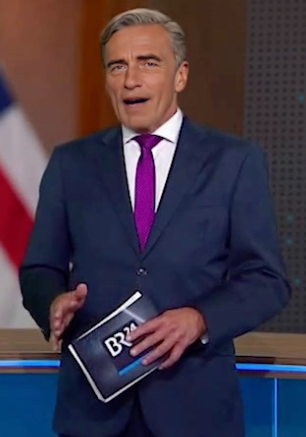
\includegraphics[width=\textwidth]{./graphics/scheider-real.png}
  \end{subfigure}
  \hfill
  \begin{subfigure}[b]{0.4\textwidth}
    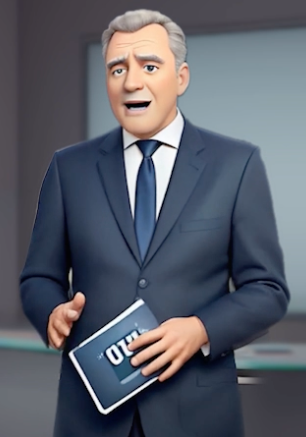
\includegraphics[width=\textwidth]{./graphics/scheider-sd.png}
  \end{subfigure}
  \caption{Stefan Scheider, Anchorman of \textit{BR24}: Real and Synthetic Adaptation.}
  \label{fig:scheider-real-sd}
\end{figure}

\begin{quotation}
"Sophisticated AI systems are increasingly everywhere. [...] However, 2023 will likely prove to be a particularly critical moment in the history of AI" \cite[p. 5]{arguedasAutomatingDemocracyGenerative2023}.
\end{quotation}

As the quoted authors state, we might be experiencing a tipping point in \gls{ai} development as more and more tools become available to a broader user base. These developments are tightly linked to the rise of OpenAI's ChatGPT and other widely adopted technologies like \gls{sd}-based \gls{t2i} generators. An output example of how future media could be produced is depicted in Figure \ref{fig:scheider-real-sd}. A more detailed description of the relevant technologies is provided in Chapter \ref{chap:background} – \nameref{chap:background}. \\
Current \gls{ai} tools are often referred to as \gls{genai}: "Generative AI is an umbrella term used for AI systems that can generate new forms of data, often by applying machine learning to large quantities of training data" \cite[p. 7]{arguedasAutomatingDemocracyGenerative2023}. One could extend this definition with the following: Besides merely generating new forms of data, \gls{genai} can be used to augment, reduce, manipulate, and mix real data with generated data in such a form that it is impossible to distinguish between real, synthetically generated (fake) data, or anything within that spectrum. \\
%\todo{P1.2. What is the specific problem?}
In the context of media production and media distribution, the developments of \gls{genai} open up an important discussion about trust and credibility. Media producers have always used synthetic content for various purposes: One can think of animated explainatory videos or other infographics. The difference is that most illustrations appear quite clearly artificial. This has now changed, as generated images and videos can look perfectly authentic and real. At the same time, these technologies are open to being used by anyone, sparking a fear of fake news. Therefore, the question for legitimate media outlets remains whether and how synthetic content will be received among their audiences. Additionally, the term "AI" itself often sparks criticism among the public due to various reasons. These effects on audiences, their mitigation, and, at the same time, the education of the broader public about technological advancements are interesting topics for media producers and outlets. Since the developments are quite recent, scarce research has been done so far.

% Second Paragraph
% CORE MESSAGE OF THIS PARAGRAPH:
%\todo{P2.1. The second paragraph should be about what have others been doing}
For the sake of completeness, negative discussions are not entirely new. So-called deepfakes (blend word of deep learning and fake news) have been around for quite some time. Papers like Facebook's 2014 DeepFace \cite{taigmanDeepFaceClosingGap2014} and the Face2Face approach by \citet{thiesFace2FaceRealtimeFace2020} date back to the year 2016. It took several years until the research gained traction among a broader audience, but at the latest in 2017, in the form of deepfake pornography and revenge porn, deepfakes hit the broader public \cite{coleAIAssistedFakePorn2017}, or as \citeauthor{westerlundEmergenceDeepfakeTechnology2019a} puts it, "After the introduction of celebrity porn deepfakes to Reddit by one user in late 2017, it only took a few months for a newly founded deepfake hobbyist community to reach 90,000 members" \cite[p. 41]{westerlundEmergenceDeepfakeTechnology2019a}. Soon afterwards, discussions arose about the implications of these technologies regarding the spread of fake news. It took some time until the fears in the domain of politics came true. In the meantime, deepfakes remained problematically present in pornography and, on the positive side, in entertainment and educational content: Jordan Peele faked Brack Obama (2018) \cite{vincentWatchJordanPeele2018}; Channel 4 emitted a fake Queen Elizabeth (2020) \cite{bbcnewsDeepfakeQueenDeliver2020}; and VFX artist Chris Ume went viral with Tom Cruise fakes (2021) \cite{vincentTomCruiseDeepfake2021}. Despite the proliferation of paid and \gls{oss} solutions for face swaps like \gls{dfl} (2019) and InsightFace Inswapper (2023), there are only a few known cases where this technology has been used in a particularly influential disinformation campaign with larger consequences. However, it goes without saying that the effect on social networks under the radar of public control might be much more significant. Some studies about these hypotheses are featured in Section \ref{chap:rel-work}. \\
Although there were other, earlier, cases as well, the first widely spread, trust-dissolving deepfake appeared in 2022, when fake news of President Zelensky of Ukraine surfaced (Figure \ref{fig:zelensky-Deepfake}). In the video, "Zelensky" demanded the soldiers to lay down their weapons \cite{zdfPropagandaImKrieg2022}. Although the Russian creators of the video later said their creation was "satire", this was certainly not clear in the original video. What had been feared for some time had become reality. The technology had been used in a political context, and probably for the first time in history, as well as in an armed conflict. A widely available, creative tool had been weaponized. Although the video seemed to have no concrete consequences for the soldiers, its role in psychological warfare cannot be denied.

\begin{figure}[h]
  \centering
  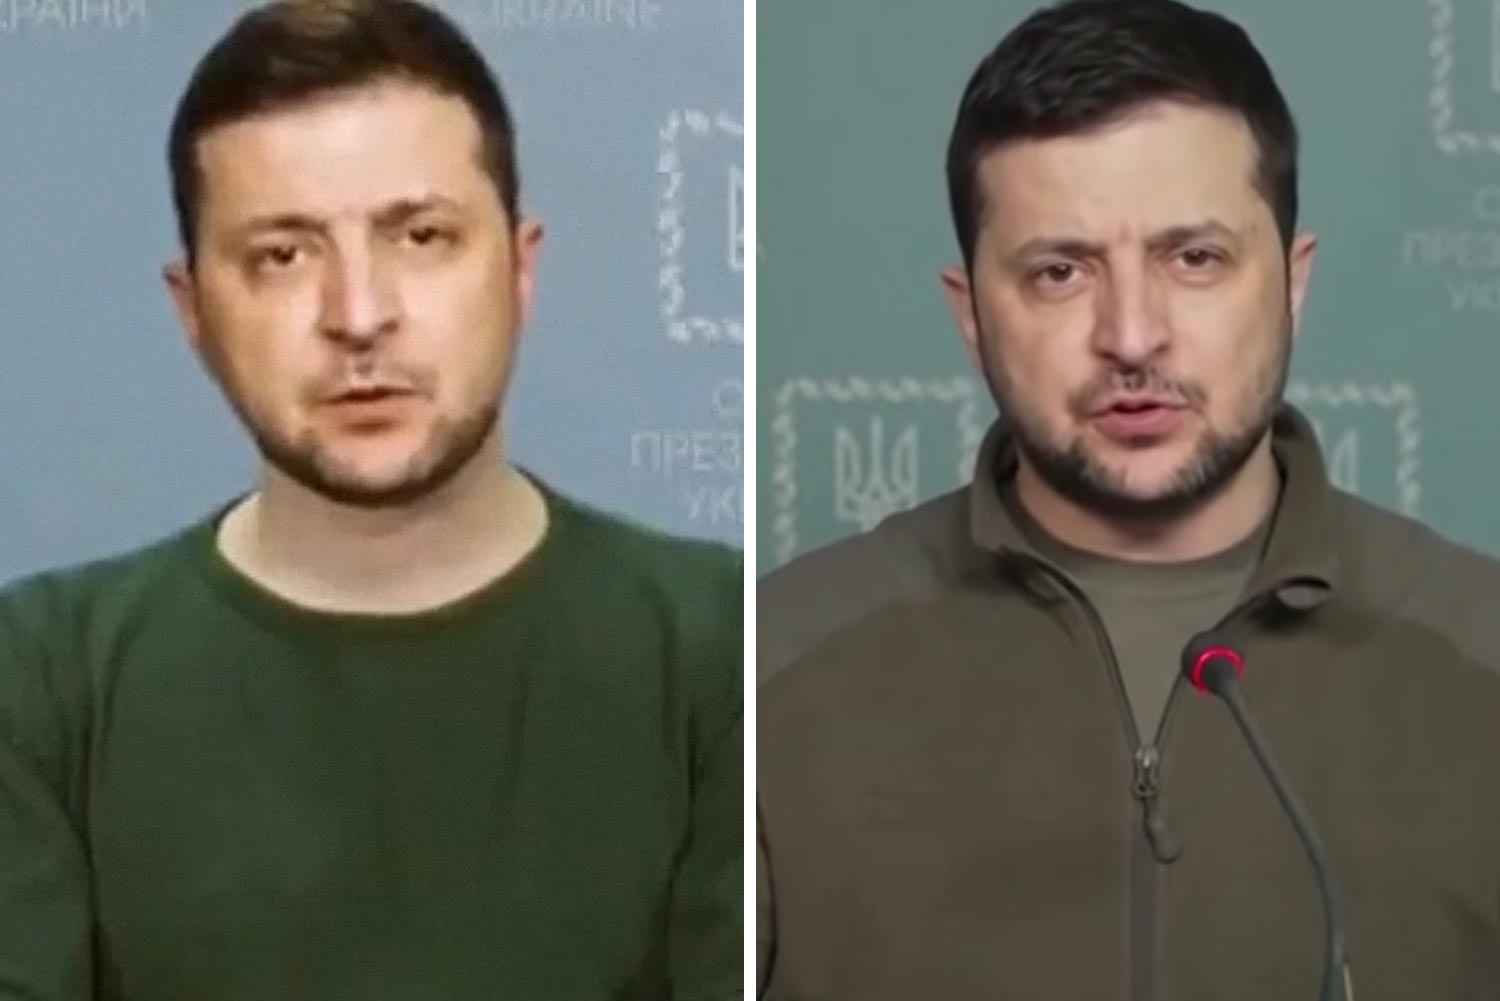
\includegraphics[width=0.6\textwidth]{./graphics/Zelensky.jpg}
  \caption{Left: Deepfake of President Zelensky. Right: Real Image of Zelensky \cite{universityofvirginiaZelenskyySurrenderHoax2022}.}
  \label{fig:zelensky-Deepfake}
\end{figure}

%\todo{P2.2. Why is the problem important? Why was this work carried out?}
Then, in the second half of 2022, several things changed in the space of \gls{ai} tools. The aforementioned \textit{simple} face swaps are now in good company in an ever-growing toolbox of \gls{ai} services: 
\begin{enumerate}
  \item GPT-enabled chat applications were released at the end of 2022.
  \item Text-to-image (t2i) generation was released in summer 2022.
  \item Excellent AI voice-cloning tools became available during 2023.
  \item Text-to-video (t2v) is advancing quickly in 2024.
\end{enumerate}
While ChatGPT is probably less relevant in the audio-visual domain, it still fuels much of the public opinion about \gls{ai} tools, as it is probably the best-known and fastest-growing software tool of all time. The other items on the list have drastically improved the quality and possibilities of how and what kind of synthetic media can be created. In recent months, there have been several reports about their use with increasing frequency. Examples of fake voices and face swaps on social media in 2023 were innumerable and can be traced back to the availability of online services such as Resemble.ai and Elevenlabs. This also leads to several nefarious use cases: To name some examples in the German context, in September 2023, a primetime news host was recreated with a fake voice in order to advertise dubious financial products (Figure \ref{fig:sievers-fake}). By using Elevenlabs' checking tool, one can quickly tell that the voice was likely created using their software.(Figure: \ref{fig:sievers-11labs}). At the end of November 2023, \textit{two} videos of German chancellor Olaf Scholz were released. One was part of a commercial campaign for a German yellow-press newspaper \cite{niemeierSpringerTrommeltMit2023}. The second was part of an art or protest project \cite{zdfKunstinstallationDeepfakeScholzVerkuendet2023}. Example images for these cases are not included, as they do not make any sense without the faked audio. 

\begin{figure}[h]
  \centering
  \begin{subfigure}[b]{0.45\textwidth}
    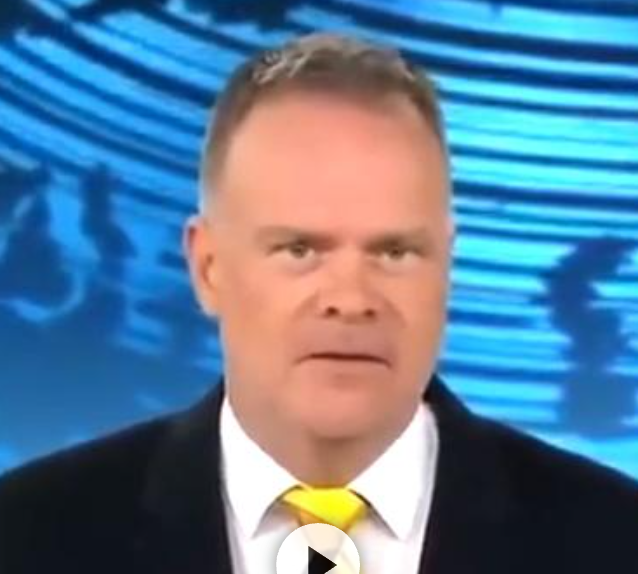
\includegraphics[width=\textwidth]{./graphics/sievers.png}
    \caption{Fake of Christian Sievers \cite{zdfDeepfakeMitZDFModerator2023}.}
    \label{fig:sievers-fake}
  \end{subfigure}
  \hfill
  \begin{subfigure}[b]{0.5\textwidth}
    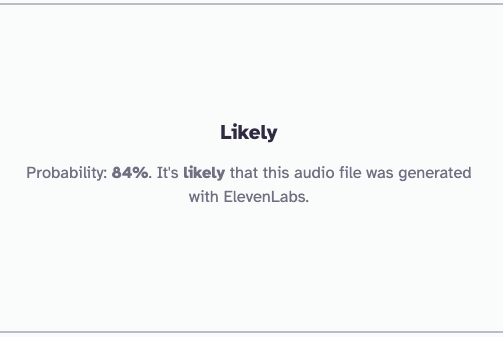
\includegraphics[width=\textwidth]{./graphics/sievers-11labs.png}
    \caption{Elevenlabs audio analysis \cite{elevenlabsAISpeechClassifier}.}
    \label{fig:sievers-11labs}
  \end{subfigure}
  \caption{Christian Sievers Deepfake and Elevenlabs Audio Analysis.}
\end{figure}

It is only logical to expect a further increase in the frequency of such content, both in the case of legitimate (commercial, education, entertainment) and illegitimate (scam, disinformation) content. An environment where both categories of content coexist is very challenging in terms of trust. For legitimate newsmakers, the question arises: How can it combat disinformation and, at the same time, use the advancements of \gls{genai} to improve production workflows? This dilemma will remain difficult to solve. The effects of these very recent technical capabilities have not yet been studied, which is why this work attempts to do so. In a time when the very existence of \gls{genai} raises trust issues with every kind of content, specifically those with synthetically generated content, any findings about synthetic media reception might be helpful in better addressing all the named issues.

% Third Paragraph
% CORE MESSAGE OF THIS PARAGRAPH:
%\todo{P3.1. What have you done?}
This paper attempts to explore the effects on potential recipients of synthetically created or AI-enhanced media in the specific context of a Bavarian/German \gls{psm} news show, namely \textit{BR24}. To be more specific, the foci of the research questions are as follows: 

\begin{enumerate}
  \item Trust and credibility in media with varying degrees of artificiality.
  \item Effects of AI disclosure by placing an AI logo watermark on the material.
  \item Determining whether there are differences within audience subgroups (age, occupation, etc.).
  \item Determining whether there are differences based on the used display size.
  \item Finding the most significant of the aforementioned variables.
\end{enumerate}

To approach these foci, an online questionnaire was conducted. The time window was 40 days, from November 6, 2023, to December 15, 2023. During this timeframe, 195 valid answers were counted. The details and results are described in Section \ref{chap:study}. Before conducting such a study, the content itself needed to be created to ensure a high degree of control over certain variables. To accomplish this, several workflows had to be established, which included several experiments with various \gls{oss} tools and how they could work together. In addition to the AI software, traditional video editing tools like Adobe Premier Pro (PrPro) and \gls{ae} were used to finalize the videos. A detailed process description of how the material was created is presented in Chapter \ref{chap:implementation}. The authors conducted this work in association with the German public broadcaster \gls{br} and the \gls{hff}. No conflicts of interest can be reported in this constellation.
%\todo{P3.2. What is new about your work?}
The tested videos were carefully designed by taking into account an extensive toolchain of available open-source technology, making it (theoretically) possible for every media producer to recreate similar results, implement (semi)automatic workflows for their media production, and conduct further experiments. As the tools are very recent developments, to our knowledge, no comparable studies have yet been conducted.

% Fourth paragraph
% CORE MESSAGE OF THIS PARAGRAPH:
The study revealed several findings regarding the relationship between synthetic media's artificiality and perceived trustworthiness. A clear correlation was identified: As artificiality increased, trustworthiness decreased. Contrary to expectations, the presence of an AI logo did not significantly impact trust, suggesting that the content's inherent qualities and presentation were crucial in shaping viewer perceptions.
These findings have profound implications for the production and dissemination of synthetic media. They underscore the need for media creators to prioritize realism and high-quality content to maintain viewer trust. Moreover, the minimal impact of AI logo disclosures on trustworthiness perceptions prompts a reevaluation of transparency practices in media production. In a broader context, this study contributes to the critical discourse on the ethical use of AI in media, highlighting the importance of ongoing research and dialogue to navigate the challenges posed by synthetic media technologies. Regarding demographics, the lack of significant differences in trust perceptions across various groups was most likely due to our study design. This aspect calls for a more granular exploration of demographic influences in future research.

\chapter{Background}
\label{chap:background}
This work focuses on the social aspects of synthetic media consumption. Therefore, we decided not to mention deep details of the technological side of machine learning in Chapter \ref{chap:rel-work} – \nameref{chap:rel-work}. However, for the study and accompanying videos, many \gls{ai} technologies were implemented. To aid the overall understanding of the whole paper, some technological background is laid out in this section.To briefly discuss the origin of the term \gls{ai}, we quote \citeauthor{haenleinBriefHistoryArtificial2019}:

\begin{quotation}
"Although it is difficult to pinpoint, the roots of AI can probably be traced back to the 1940s, specifically 1942, when the American Science Fiction writer Isaac Asimov published his short story \textit{Runaround}" \cite[p. 6]{haenleinBriefHistoryArtificial2019}. 
\end{quotation}

Along with science fiction, practical science was evolving during World War II. After Alan Turing famously engineered a computer to crack the Enigma cryptography, Turing published his paper, "Computer Machinery and Intelligence," where he described how to create intelligent machines and, in particular, how to test their intelligence \cite{turingCOMPUTINGMACHINERYINTELLIGENCE1950}. In the following years, the term "artificial intelligence" rose to more prominence, most notably at Dartmouth College, where Marvin Minsky and John McCarthy hosted the \textit{Dartmouth Summer Research Project on Artificial Intelligence (DSRPAI)} in 1956 \cite{flasinskiHistoryArtificialIntelligence2016}. \\
The different times when \gls{ai} experienced its highs and lows are often referred to as the four seasons of AI. Spring, representing the dawn of \gls{ai}, was followed by summer. After the events at Dartmouth College, a great deal of funding from U.S. institutions such as DARPA and the RAND Corporation went into AI research. Without going into too much detail about various developments, one can state that this first dawning abruptly ended around 1973 when governmental spending was cut due to a lack of advancements. The first \gls{ai} winter is often credited to Marvin Minsky and Seymour Papert, who published their famous book \textit{Perceptrons} \cite{minskyPerceptronsIntroductionComputational2017} in 1969, in which the authors showed the strong limitations of perceptrons, for example, the inability to compute some logical functions like XOR. As a result, many \gls{ai} researchers concluded that the study of neural networks was not promising \cite{flasinskiHistoryArtificialIntelligence2016}. \\
\Citeauthor{haenleinBriefHistoryArtificial2019} stated that, although the Japanese government began to heavily fund \gls{ai} research in the 1980s (to which the U.S. DARPA responded with a funding increase as well) no further advances were made in the following years. This can only be partially held true because some progress had to be made before the second \gls{ai} summer came around, notably multi-layer perceptrons – and therefore deep neural networks – in 1965, backpropagation in 1970, convolutional neural networks in 1979, autoencoders in 1986, and generative adversarial networks (GANs) in 1990, to name just a few \cite{schmidhuberAnnotatedHistoryModern2022}. \\
The current \gls{ai} summer arrived with \citet{krizhevskyImageNetClassificationDeep2012} and their significant advancements in image recognition using a convolutional neural network called AlexNet. Their network performed considerably better than the previous state of the art. In 2015, AlphaGo became the first \gls{ai} to beat grandmasters in the game Go. Besides the image recognition domain, text and natural language processing received huge performance improvements with \citetitle{vaswaniAttentionAllYou2023} and the authors' transformer architecture in 2017. Text-to-speech (TTS) also benefited from transformer research, with major advancements \cite{wangTacotronEndtoEndSpeech2017}. To name one of the most recent advancements, diffusion-based approaches gave the powerful \gls{t2i} generator Stable Diffusion its name \cite{rombachHighResolutionImageSynthesis2022}. A chronological overview of the model developments is depicted in Figure \ref{fig:timeline-models}. As scientific advancements have been numerous, so have their practical implementations. Those relevant to this work are briefly described below.

\begin{figure}[h]
  \centering
  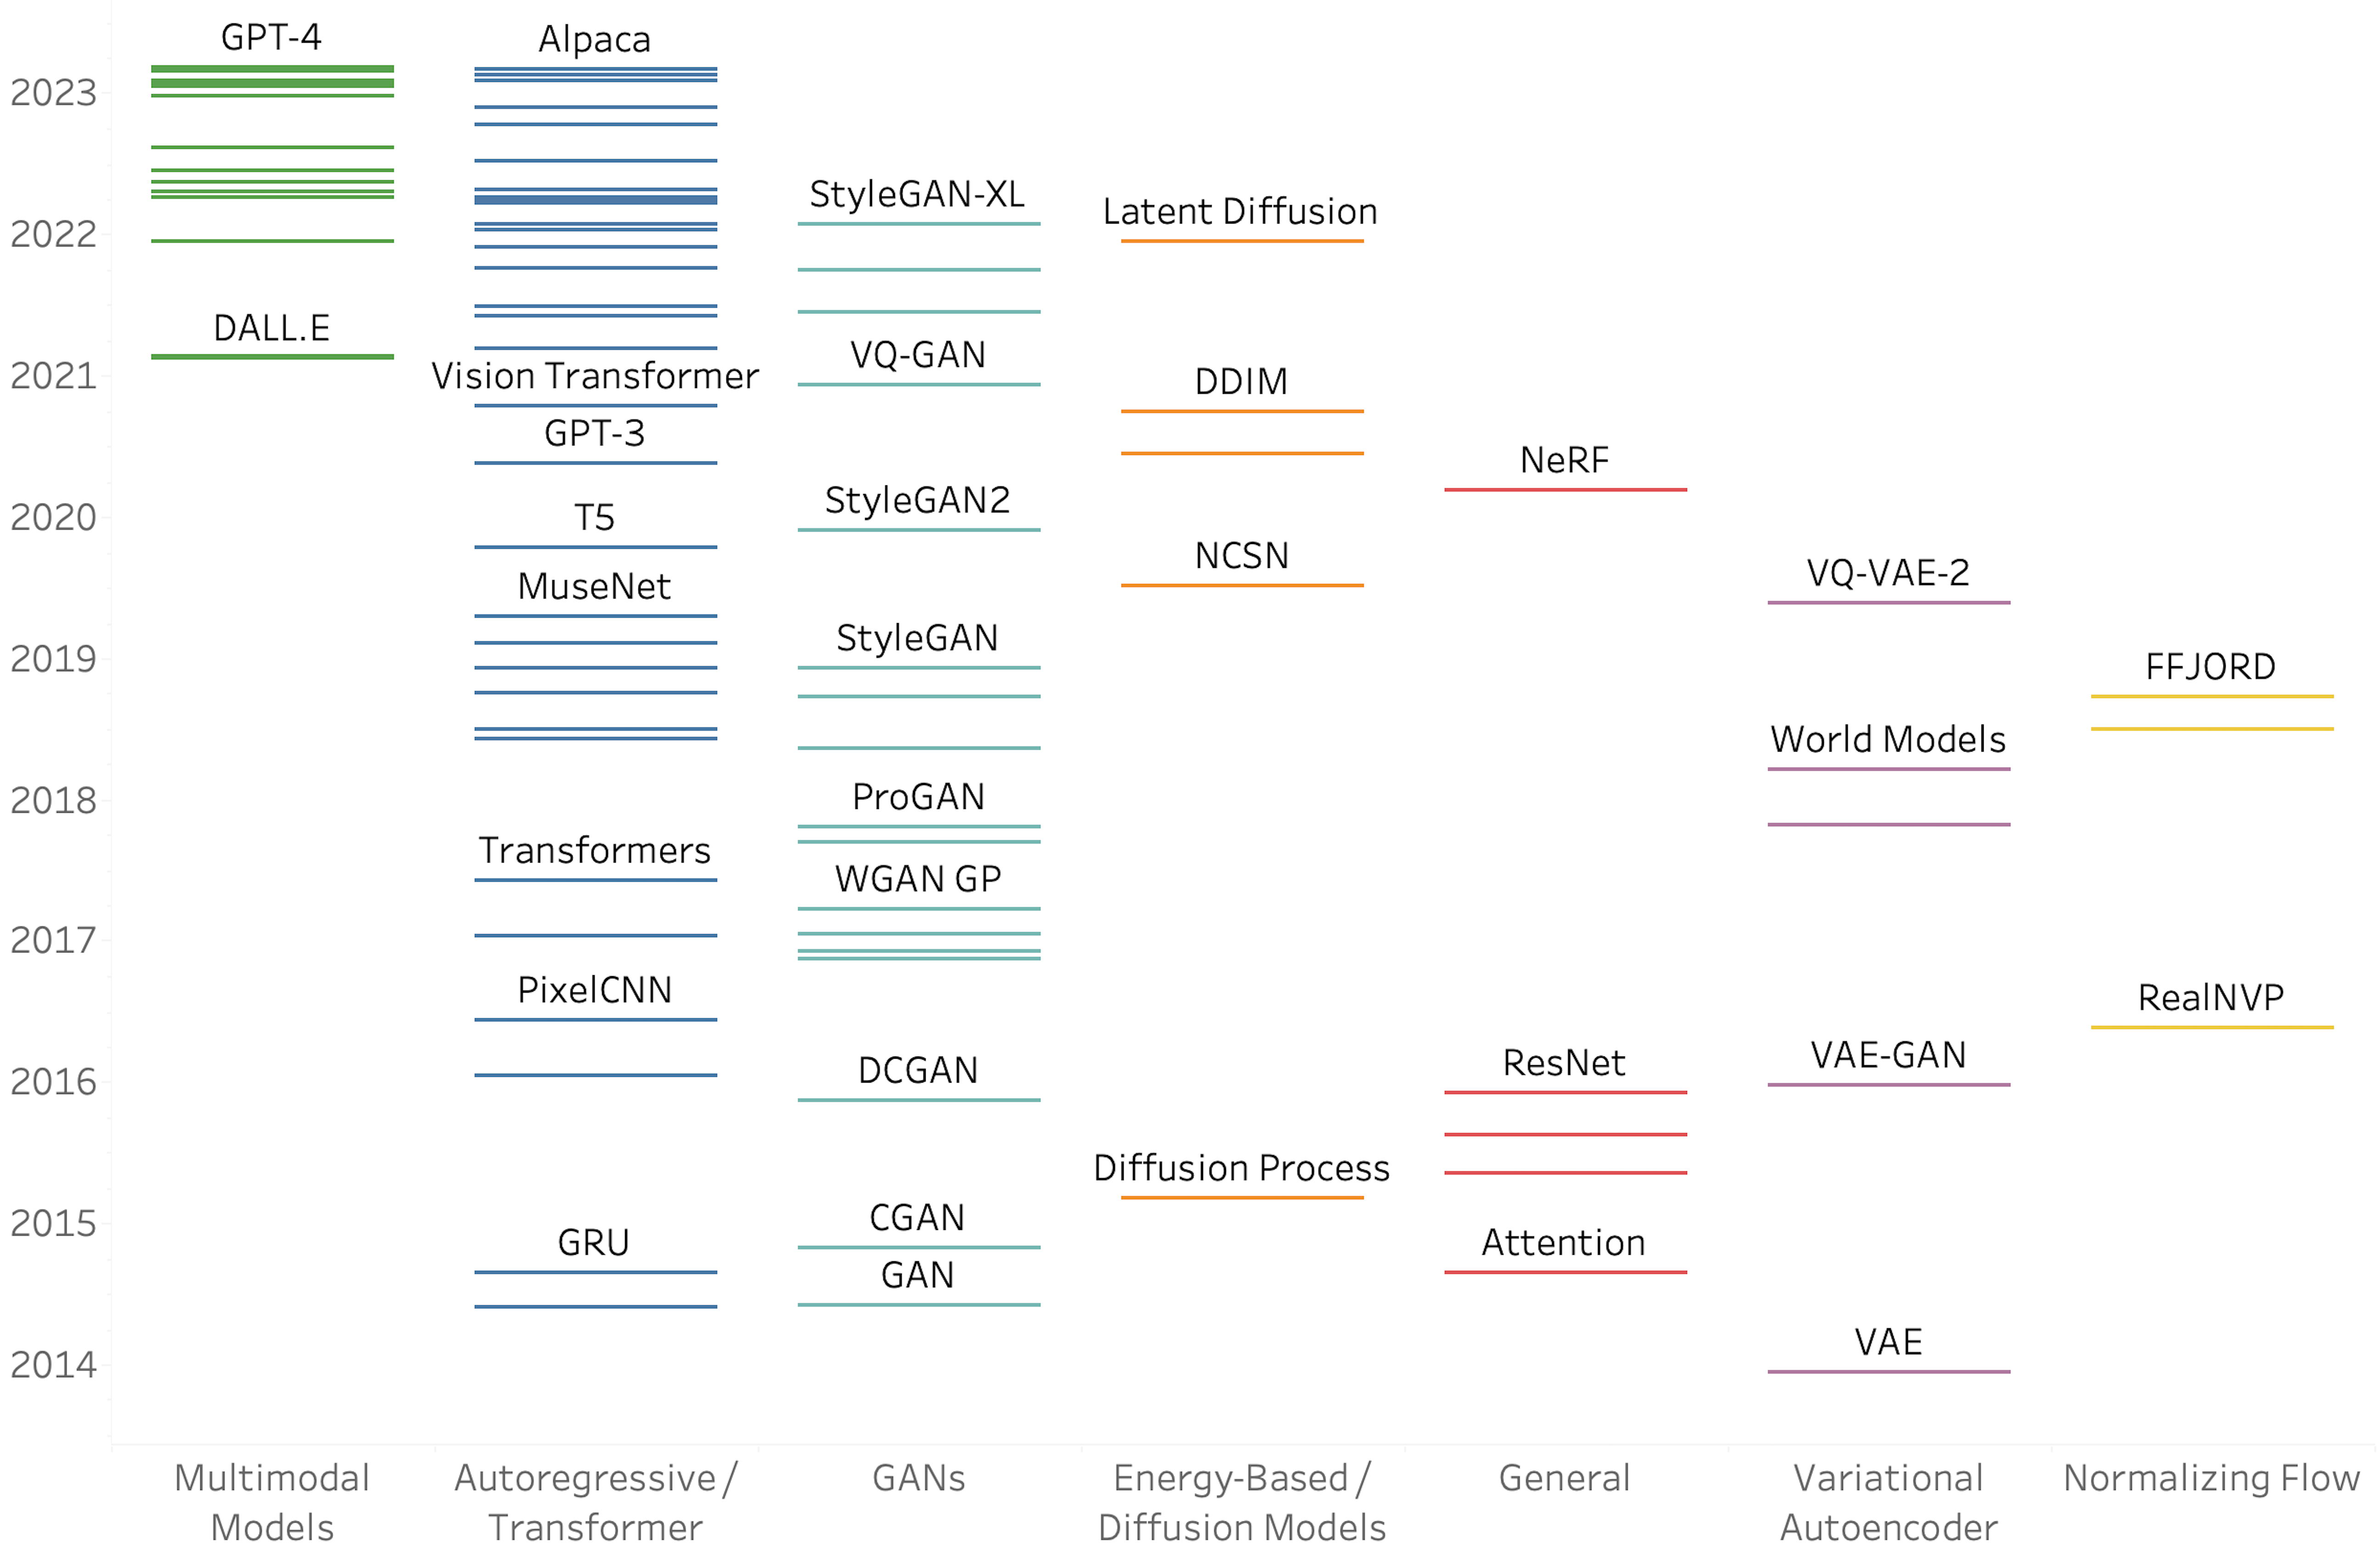
\includegraphics[width=1\textwidth]{./graphics/Timeline_of_generative_models_by_type.png}
  \caption{Timeline of Generative Models by Type \citet{garcia_penalvo_2023_8165255}.}
  \label{fig:timeline-models}
\end{figure}

\section{Generative AI}
\label{sec:genai}
The term \gls{genai} was briefly mentioned in the introduction, but for a better understanding, the term shall be examined more deeply to avoid misunderstandings and ambiguity. There is no globally agreed definition for "generative AI" \cite{garcia-penalvoWhatWeMean2023}. In technical terms, a generative model, as described with a \gls{gan}, refers to specific subforms of neural network architecture.

\begin{figure}[h]
  \centering
  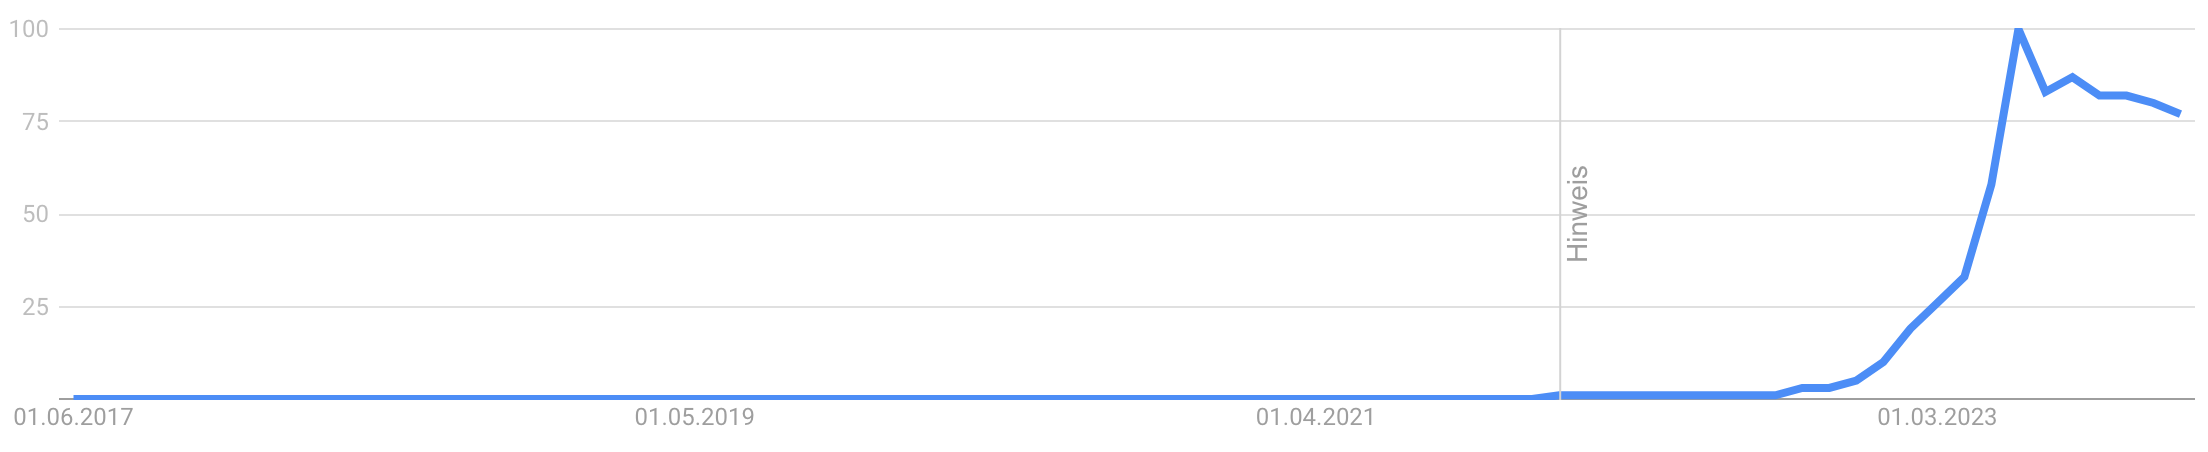
\includegraphics[width=1\textwidth]{./graphics/gtrends_genAI_1712-2312.png}
  \caption{Google Trends of "Generative AI" from December 2017 to December 2023 \cite{googletrendsGoogleTrendsQuery}.}
  \label{fig:gtrend-genai}
\end{figure}

It is unlikely that the broader public refers to the same, rather technical context. It is more likely that the meaning is less about technical implementations and more about how the end user utilizes the software. If things can be generated using \gls{ai}, they must be named \textit{generative} \gls{ai}. This notion can be supported by Google trends for "generative AI" as depicted in Figure \ref{fig:gtrend-genai}. The search requests begin to rise in October 2023 and then climb high from December 2023 onward. This fits with the release of ChatGPT and the spread of image generation software and accompanying media coverage. \\
In the following, the term "\gls{genai}" is used in the way the broader public understands it and not as the narrow technical definition. Technical details are discussed and elaborated further. 

\section{Uncanny Valley}
Besides the technical terms, we also need to quickly cover the concept of the uncanny valley, first described by Masahiro Mori, a robotics professor at the Tokyo Institute of Technology. He hypothesized that a person's response to a humanlike robot would abruptly shift from empathy to revulsion as it approached, but failed to attain, a lifelike appearance \cite{moriUncannyValleyField2012}. Some examples of this spectrum are given in Figure \ref{fig:uncanny-valley}.

\begin{figure}[h]
  \centering
  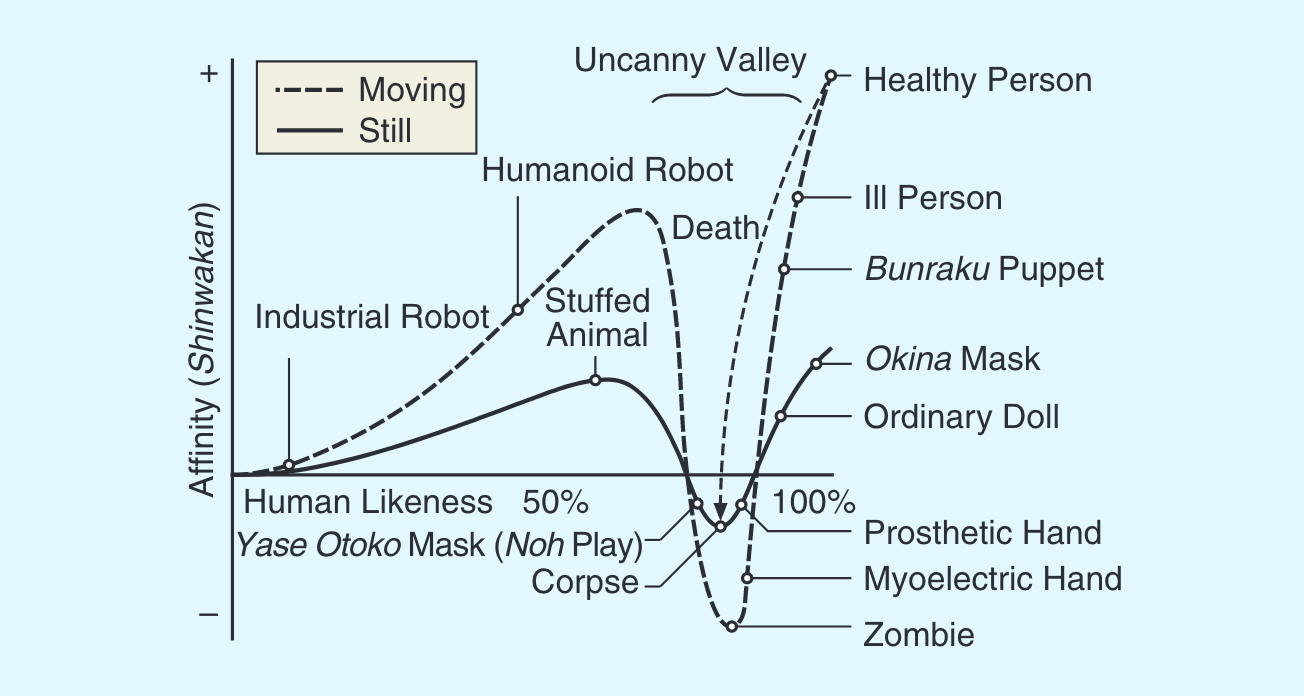
\includegraphics[width=0.9\textwidth]{./graphics/uncanny-valley.png}
  \caption{Uncanny Valley According to Masahiro Mori \cite{moriUncannyValleyField2012}.}
  \label{fig:uncanny-valley}
\end{figure}

Knowledge about the uncanny valley is important because the concept can be widely adopted in other domains besides robotics. We took its effect into account for each test case within our study. As we investigate trust in \gls{ai}-aided news, we must consider that a loss in trust could also be related to uncanny valley effects. We address how we handled the effect of the uncanny valley in our study design in Section \ref{sec:study design}.

\section{LLM-based Chatbots}
A \gls{llm}-based chatbot (ChatGPT) was used at several points to conduct this research. Especially during the software development phase (Chapter \ref{chap:implementation}) and the study design (Section \ref{chap:study}), ChatGPT was consulted to speed up the processes greatly. \\ 
For the content generation of our study videos, it did not play any role and thus is not discussed as deeply as the other technologies. However, we must consider the mere existence of ChatGPT in the context of the time. As discussed in Section \ref{sec:genai}, the public's attention towards AI tools has been tremendously accelerated by the broad availability of ChatGPT. When compared to the slow and steady increase of Google trends regarding the term "deepfakes" in Figure \ref{fig:gtrend-deepfakes}, a disruptive tendency can clearly be seen, overlapping with the emergence of ChatGPT and \gls{t2i}-generators. As a standing fact, it must be considered how an individual's \gls{ai} education could influence his or her response to the study.

\section{Face Swapping}
\label{sec:face-swapping}
Similar to the previous section regarding ChatGPT, face swaps were not used directly within this project to create media but have played a very important role in shaping public opinion about synthetic media. As mentioned in the introduction, face swaps initially introduced the \textit{deepfake}, which is still used today. This fact often shifts synthetic media toward having a negative connotation. \\
Besides problems with deepfake pornography and revenge porn, the first publicly recognized deepfakes were those of Obama/Jordan Peele face swaps in 2018 \cite{vincentWatchJordanPeele2018}. \citet{hancockSocialImpactDeepfakes2021} stated that the Obama video is likely the most canonical, if not the original, deepfake video. This is supported by a strong bump in Figure \ref{fig:gtrend-fake-news}. The video featured filmmaker Jordan Peele impersonating Barack Obama using swear words and insulting President Trump. By adding a face swap, the scene appears very convincing. The political dimension of the video brought significant public attention to the previously less-known topic of deepfakes.

\begin{figure}[h]
  \centering
  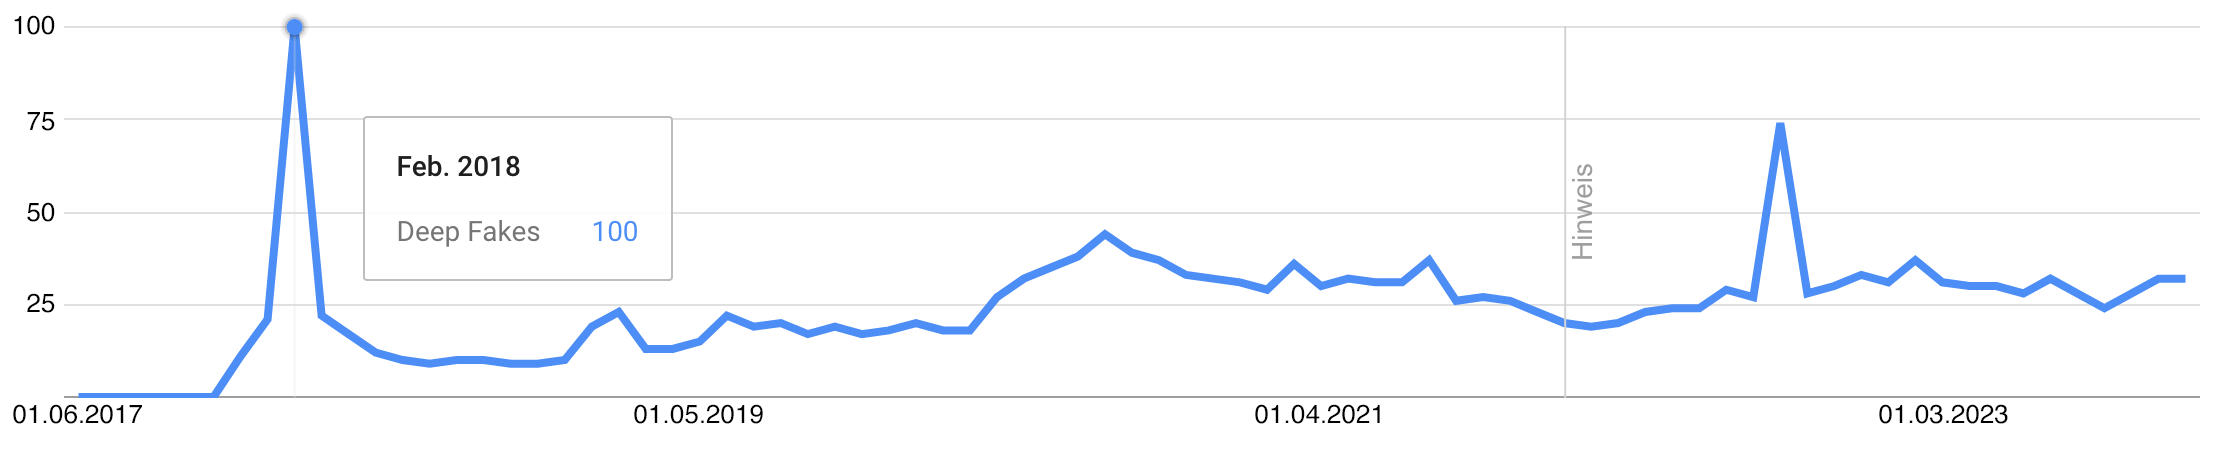
\includegraphics[width=1\textwidth]{./graphics/gtrends_deepfake_1712-2312.png}
  \caption{Google Trends of "deepfakes" from December 2017 to December 2023 \cite{googletrendsGoogleTrendsQuerya}.}
  \label{fig:gtrend-deepfakes}
\end{figure}

Prior to this paper, extensive experiments have been conducted with different face swap toolkits. In the end, no face swaps were performed for the study examples. The reason for this decision lies in the study design: Briefly captured, a controlled environment was needed in order to rule out as many disruptive factors as possible. The TV news setup was chosen, as it provided a steady setting. In this case, face swaps were not needed. They could have been optionally used to improve the final quality of the rendered faces, but due to time constraints, this approach was not carried out. This idea is picked up again in Section \ref{sec:lips} when the quality of lip remapping is addressed.
Still, the findings regarding face swaps are interesting in the background context of this work and thus are included briefly in the following paragraphs.

\subsection{DeepFaceLab}
\begin{figure}[h]
  \centering
  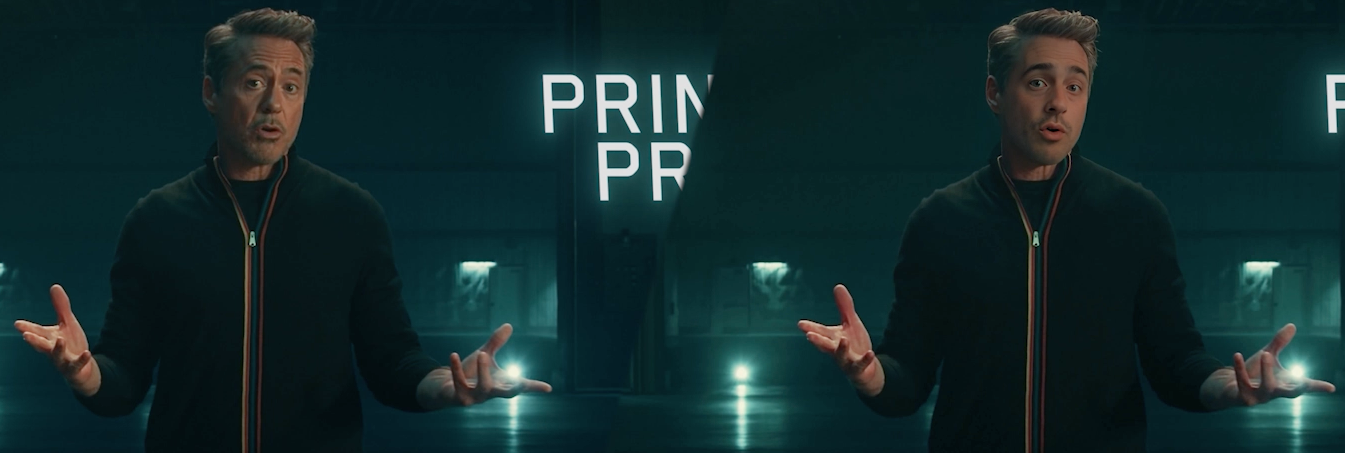
\includegraphics[width=1\textwidth]{./graphics/dfl-demo.png}
  \caption{DeepFaceLab Test Result from September 2021.}
  \label{fig:dfl-sample}
\end{figure}
By far, the leading software for face swapping is \gls{dfl}. It is also one of the first and oldest in the growing line of synthetic media creation tools. It encompasses a broad workflow in order to create high-end face models. According to the commit history, \gls{dfl} came into existence in June 2018 \cite{perovCommitsIperovDeepFaceLab}. Without being able to say it with certainty, DFL's success might also lie in its proximity to pornography. The reason for this suspicion is that the main guide for how to work with \gls{dfl} is hosted on a subpage of \textit{mrdeepfakes.com}, which claims to be the largest deepfake porn site. To our knowledge, these topics were rarely addressed by the authors of the software. This is highly problematic, as a lot of psychological pain and stress have been inflicted by the technology. As of November 2023, the software has been phased out of development and archived by the lead developer without providing any reasons. This probably has to do with the upcoming release of newer, faster methods of face swapping discussed in Section \ref{sec:roop}. For the high-end workflow, \gls{dfl} can still be used, but there are also other alternatives. \textit{FaceSwap}, actually the first tool introduced in 2017, is still under development.

The terms \textit{\gls{dfl-dst}} and \textit{\gls{dfl-src}} are to be understood in such a way that the \gls{dfl-dst} is the face that will drive the final face. The \gls{dfl-src} is the face that is being faked onto the \gls{dfl-dst}. The standard workflow for creating a DFL model is as follows:\\
(1) \textbf{Data gathering} involves finding the right material with which to train the models. High-resolution images of both the \gls{dfl-dst} and the \gls{dfl-src} are required but can be easily found online in videos. The final face resolution usually ranges from 128x128 up to 512x512 pixels. The videos used for data gathering should be of such quality that the required face size can be extracted from the gathered videos. It is very important that the images cover a wide variety of facial angles, expressions, and lighting situations. Usually, around 8.000 facial images are enough for a good fake. \\
(2) During \textbf{face extraction}, faces of the desired size are detected in video frames and extracted. Furthermore, facial alignment data is embedded into the images as metadata, as it is required for the training process. \\
Afterwards, (3) \textbf{sorting and data refinement} are needed to ensure that face alignments have been correctly identified. This step also involves sorting out unwanted images. Exclusion criteria include blurriness or wrongly detected faces, for example. \\
Next, (4) \textbf{mask segmentation} comes into play. Here, the face gets masked out by a tool. This involves drawing manual face masks to fit the \gls{dfl-dst}s and \gls{dfl-src}s face geometry needed for easier merging later on. This way, obstructions in front of the face can be masked so that the model learns to mask them out as well during inference, also called merging.  This concludes the pre-processing in most cases.\\
Afterwards, the (5) \textbf{training} can begin. Training can take, depending on hardware, resolution, and dataset size, some days up to weeks or months to conclude. The training itself is divided into multiple stages where different hyperparameters have to be adjusted. \\
After training, the final \gls{dfl-dst} can be (6) \textbf{be merged} with the synthetically generated face. An example of the generated quality can be seen in Figure \ref{fig:dfl-sample}.

\begin{figure}[h]
  \centering
  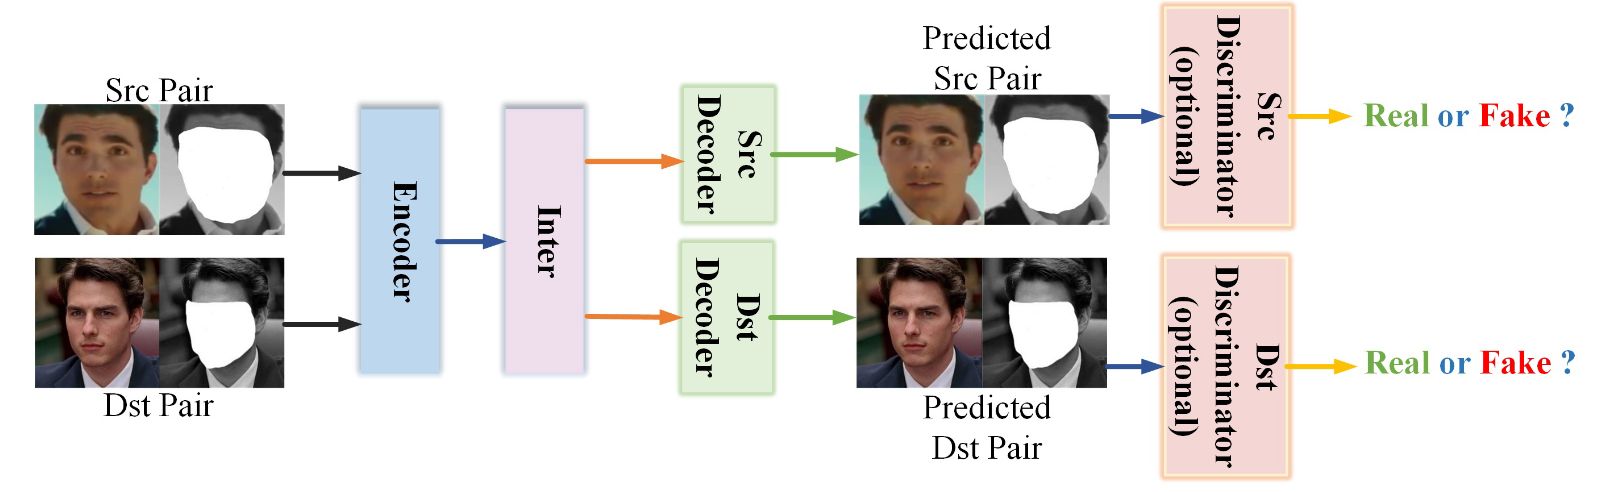
\includegraphics[width=1\textwidth]{./graphics/df-model-arch.png}
  \caption{Deepfake Model Architecture Diagram \cite{perovDeepFaceLabIntegratedFlexible2021}.}
  \label{fig:df-model-diagram}
\end{figure}

\gls{dfl} face swaps are based on an autoencoder architecture like that described in Figure \ref{fig:df-model-diagram}, although in the meantime, several subvariants have been developed. Autoencoders are notoriously known for their inability to create sharp images. Because of that, face-upscaling GANs are added to the training process. As can be seen, the use of \gls{dfl} is quite complex and time-consuming. On the other side, it provides a great degree of freedom compared to newer and simpler methods.

\subsection{Inswapper}
\label{sec:roop}
Developed on the foundations of the Insightface Face Analysis Project \cite{insightfaceInsightFaceWebsite} Inswapper provides a very easy way to swap faces without the need for any training before inference. The workflow is as simple as loading a targeted video as well as a source image into the \gls{gui} of Roop \cite{sangwanRoop2023} and waiting for the software to create the merged video. The model used in the background is closed source and thus cannot be retrained. Besides the enormous acceleration of the whole process, the lack of customization is the biggest drawback in comparison to \gls{dfl}. Overall, the quality of the generated Inswapper faces is quite good. However, the quality of the generated faces drops significantly in situations where the face is obscured or angled in profile towards the camera. Some examples are included in Appendix \ref{chap:insightface-demos}. Although it was not stated specifically by the \gls{dfl} developers, such rapid advancements in face swap technology might be one reason that \gls{dfl} was discontinued.

\section{Image Generators}
\label{sec:stable-diffusion-bg}
\begin{figure}[h]
  \centering
  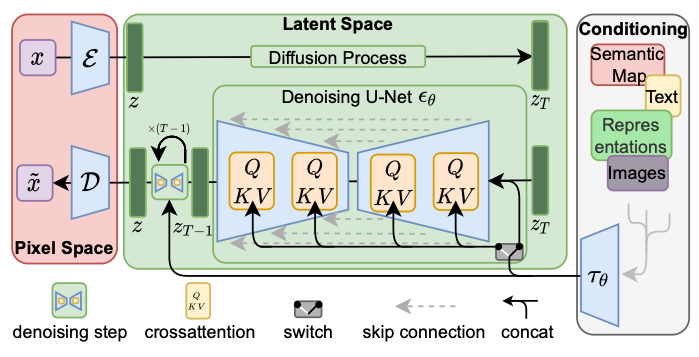
\includegraphics[width=0.9\textwidth]{./graphics/latent-diffusion.png}
  \caption{Latent Diffusion Model \cite{rombachHighResolutionImageSynthesis2022}.}
  \label{fig:ldm-arch}
\end{figure}

\citet{rombachHighResolutionImageSynthesis2022} released their \gls{ldm} (Figure \ref{fig:ldm-arch}) in the summer of 2022 and started a huge movement in computer graphics. We will not go into further details about the inner workings of the \gls{ldm} workflow, but a brief overview is given in Appendix \ref{app:diff-workflow}.\\
The open-sourced workflow has been quickly adopted in multiple products and fuels several companies such as \textit{Midjourney, Pika-Labs, Runway, DI-D}, and many more. Even more interesting than the appearance of commercial solutions is the fact of how quickly a huge open-source community grew from the \gls{sd} project. Currently, there are around a dozen different \gls{gui} projects available for \gls{sd}, some even featuring extensions within the \gls{gui}. The largest, \textit{\gls{auto1}}, lists \textbf{269} community extensions that greatly extend the functionality in different directions, for example, towards video generation. The project was initiated in August 2022, has 24,000 forks and a 121,000-star rating, which is an impressive rate of development \cite{AUTOMATIC1111StablediffusionwebuiStable}. \\
Midjourney, probably the best-known commercial solution, works over a Discord chatbot interface and currently has around \textbf{17.3} million registered users on their channel \cite{midjourneyJoinMidjourneyDiscord}.

Besides the development of image generator software, there is also a thriving community for model development and fine tuning the so-called \gls{lora} models. These are then shared on platforms such as \gls{hf} or, more prominently, Civitai.com. While \gls{hf} is focused on the developer side of models, Civitai.com can also be seen as a sort of social network where user-generated content in the form of generated images is showcased. Civitai hosts "thousands of high-quality Stable Diffusion models", as the site currently states \cite{CivitaiHomeOpenSource}. \gls{lora}s are especially interesting as they are very small (several megabytes) compared to full-fledged models (several gigabytes). LoRas help in fine-tuning the larger models towards a specific goal. Because LoRas are so small, they can be shared very easily within the community. It goes without saying that this sort of plug-and-play models are also well suited and used for pornographic purposes as well. Different from the earlier-mentioned of mrdeepfakes.com, civitai.com features nudity filters and seeks to create a safer space for every kind of content. A public debate has already started about whether AI-generated pornography will replace pornography one day. Surely, the ethical concerns could fill a paper on their own and thus require separate research. However, some discussions are mentioned as related work in Chapter \ref{chap:rel-work} – \nameref{chap:rel-work}.

Latent diffusion models act not only as the core technology but also as a platform, and the adoption speed and extensibility of both the technology and the community indicate that a disruption is taking place here. In the context of this paper, an \gls{sd} workflow is used to generate test videos in the style of computer animation (Figure \ref{fig:scheider-real-sd}). The used workflow is featured later in Section \ref{sec:sd-video}. Furthermore, \gls{svd} has been released in late 2023; it showcases the rapid rate of advancement in the field of \gls{ldm}s. In just one year, \gls{t2i} generators became text-to-video generators as well.


\section{Lip Remapping}
\label{sec:lips}
After discarding the previously discussed whole-face swaps using \gls{dfl} as a meaningful tool for the study, lip remapping was chosen as one of the main visual technologies for this work. The basis for many videos was real recordings from a news show. After creating a synthetic voice (refer to Sections \ref{sec:tts} and \ref{sec:v2v}) the proper mouth movement needed to be recreated to make the videos somewhat convincing. \\
To accomplish a satisfying result, multiple tools needed to be chained together. First and foremost, there is \textbf{Wav2Lip (\gls{w2l})}. Based on the research of \citet{prajwalLipSyncExpert2020}, a code implementation is provided on GitHub \cite{mukhopadhyayWav2LipAccuratelyLipsyncing2023}. The code was adapted to fit the workflows for the creation of the study videos and explained in further detail in the Chapter \ref{chap:implementation} – Implementation. The \gls{w2l} project is also one of the older synthetic media tools, released in 2020.

\begin{figure}[h]
  \centering
  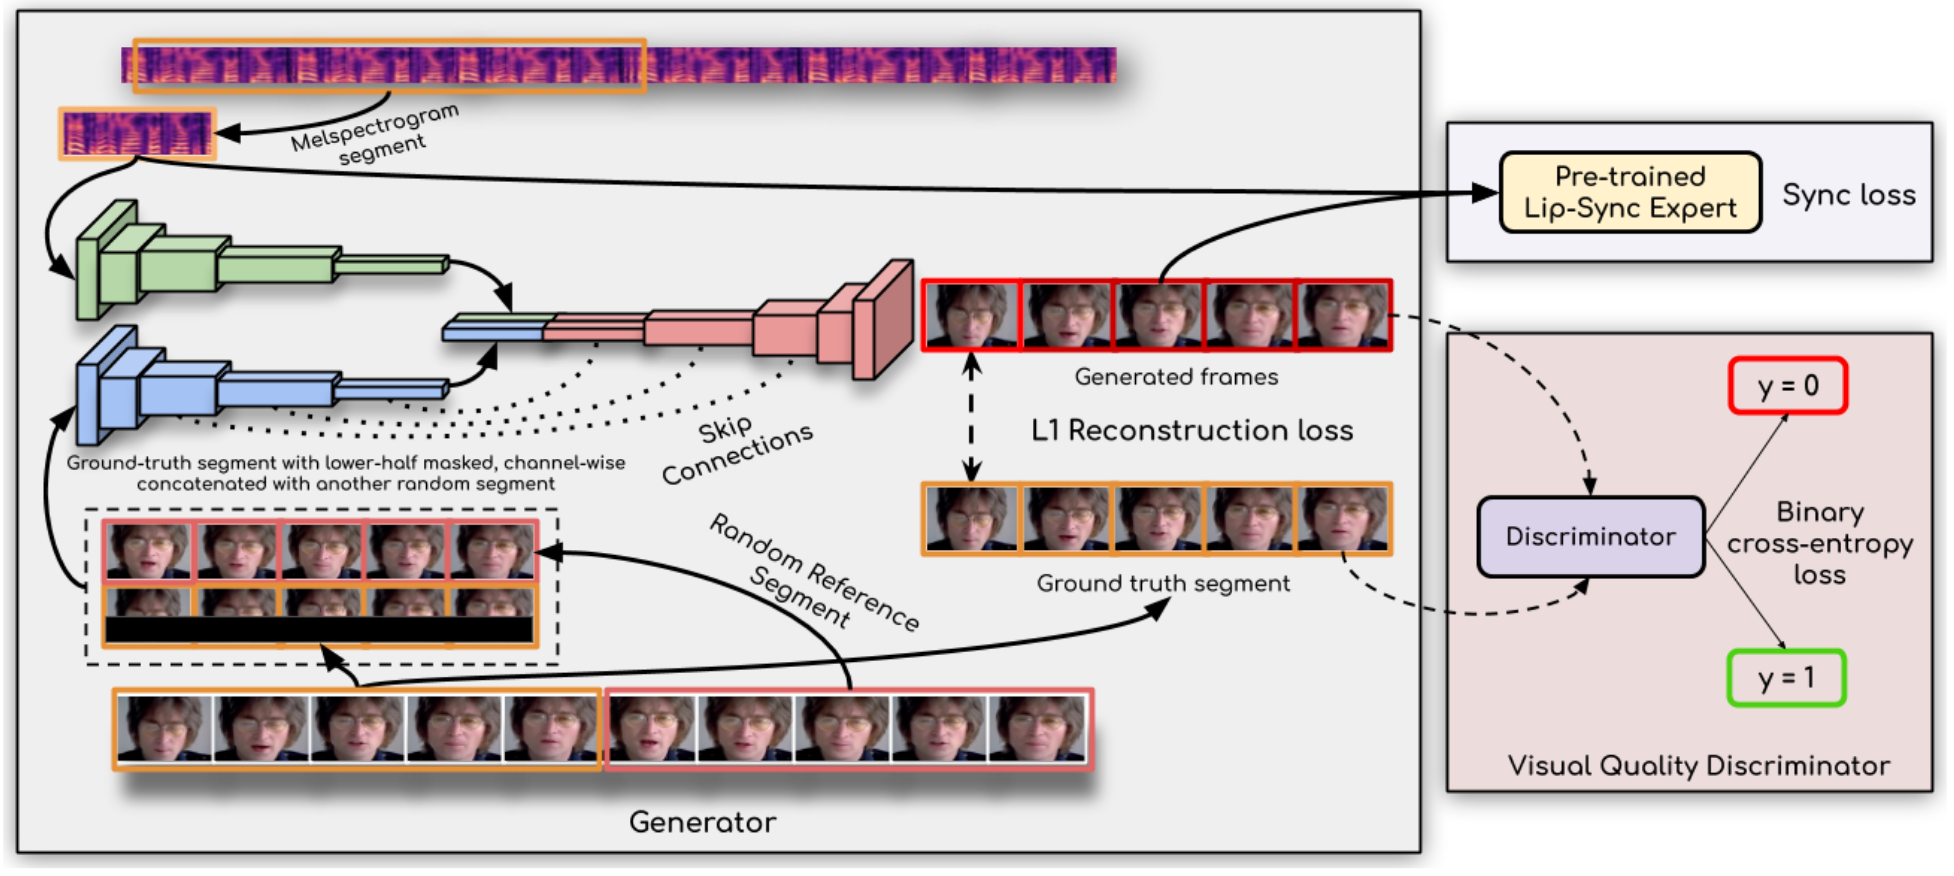
\includegraphics[width=1\textwidth]{./graphics/w2l-arch.png}
  \caption{Wav2Lip Architecture.}
  \label{fig:wav2lip-arch}
\end{figure}

The architecture (Figure \ref{fig:wav2lip-arch}) is based on a GAN generator-discriminator approach, adding an additional lip-sync-expert discriminator, which improved the results significantly in comparison to previous methods. \\
Unfortunately, the available public \gls{w2l} model has been trained on a face resolution of only 96x96 pixels, which is insufficient for a convincing effect. To address this issue, a face-upsampling GAN was added to the workflow to increase the facial resolution. The upsampling was performed using the public \textbf{GFPGAN} implementation based on the works of \citet{wangNeuralSourcefilterbasedWaveform2019}. The results can be seen in Figure \ref{fig:wav2lip-demo}: To the right, one can see the original actor; the middle shows a \gls{w2l} result where the mouth region is blurry; and the left depicts the GFPGAN upsampling. The GFPGAN workflow splits the blurry video into individual frames and upsamples each face individually. This introduces flickering artifacts in the face due to small inconsistencies after upsampling that look like flickering when played back at 25 \gls{fps}. This issue can be mitigated with further post-production.

Overall, the process of creating the lip remapping is rather slow. One 20-second video takes over five minutes to export. The additional post-production and compositing of all audio and video sources back together takes around 20 minutes after the workflow is repeated multiple times. Using GFPGAN was not the only option to improve the face quality. As mentioned in Section \ref{sec:face-swapping} we could have used \gls{dfl} on top of the \gls{w2l} output to sharpen the result with a full face swap. The method has been tested on other occasions and works quite well. It also does not have issues with face flickering. On the other hand, creating a \gls{dfl} model is very time consuming, especially if it needs to be good. The processes within this work needed to be somewhat practical for everyday use in a media company. If every lip-remapped actor needs their own \gls{dfl} model trained, it is not practical. One-image-swap solutions, like the previously described Inswapper, do not improve the quality of the \gls{w2l} outputs. \\
Ideally, one would work with a higher-resolution \gls{w2l} model or newer approaches like those from \citet{guptaGeneratingUltraHighResolution2023}. The authors state that their approach delivers great results at 768 x 768 pixels compared to \gls{w2l}'s 96 x 96 resolution. Unfortunately, there was no available code implementation for the paper at the time, so it could not be tested.

\begin{figure}[h]
  \centering
  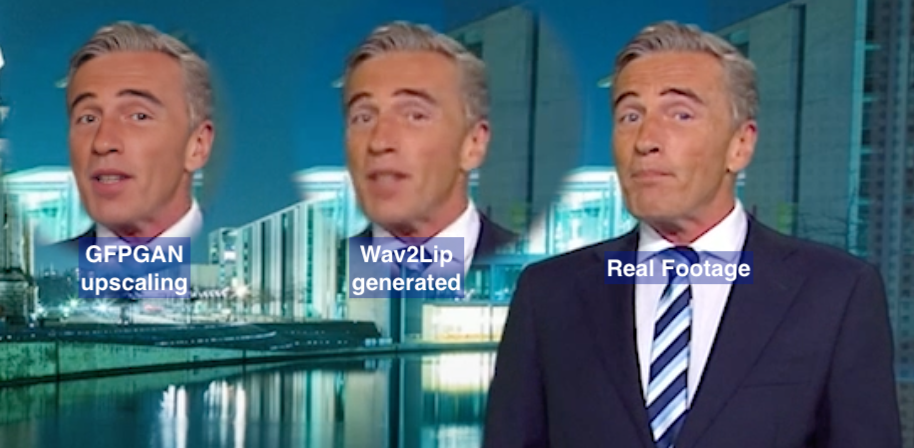
\includegraphics[width=0.9\textwidth]{./graphics/wav2lip/wav2lip-demo.png}
  \caption{Lip Remapping Workflow, Described from Right to Left.}
  \label{fig:wav2lip-demo}
\end{figure}

\section{Text-To-Speech}
\label{sec:tts}
To cover the audio component of the videos, \gls{tts} is used. Although there are plenty of web-based solutions (\textit{elevenlabs.io, resemble.ai}), one goal of the project is to only use \gls{oss} solutions. Regarding \gls*{tts}, the decision was made to use \textbf{CoquiTTS}, a library for \gls{tts} generation with pretrained models in 1,100+ languages \cite{erenCoquiTTS2021}. CoquiTTS, which developed out of a Mozilla project, is community-driven but also provides a \gls{saas} called Coqui Studio. In comparison to the earlier mentioned \gls{sd} community, Coqui's community is not as large, and the community support and documentation are worse. However, there is at least some documentation about training a new voice. The results were satisfying but certainly leave plenty of room for improvement compared to state-of-the-art commercial solutions.

One of the biggest challenges in implementing \gls{tts} was the gathering and pre-processing of the training data. In exchange with the community, a dataset size of around four hours of speech was required to obtain decent results. The difficulty did not lie in getting the raw data; this was easily obtained from the archives of the \gls{br}. In order to train the \gls{tts} model, the data needed to be structured in a special format. Audio segments needed to be under 10 seconds in length, and each audio file needed accompanying transcription in a text file. To solve these issues in four hours of content, a toolkit was developed to facilitate data preprocessing, which is explained in detail in Section \ref{sec:dvt}.

\begin{figure}[h]
  \centering
  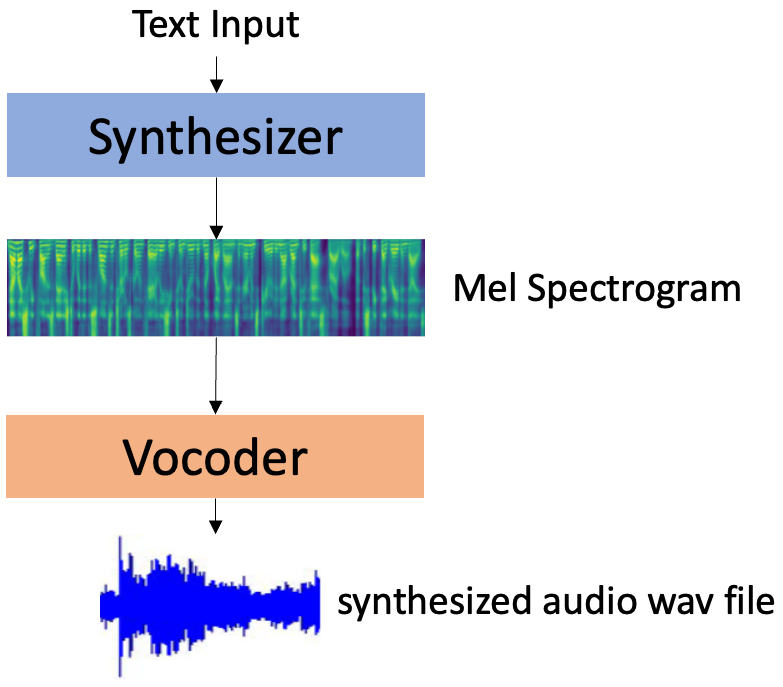
\includegraphics[width=0.5\textwidth]{./graphics/tts/tts-workflow.png}
  \caption{Basic Text-To-Speech Workflow \cite{jemineRealTimeVoiceCloning2019}.}
  \label{fig:tts-explainer}
\end{figure}

Usually, \gls{tts} is accomplished by using multiple stages of training multiple models. A basic overview of how they work together can be seen in Figure \ref{fig:tts-explainer}. The input text is encoded as a mel spectrogram by the synthesizer. Based on these mel spectrograms, the vocoder then generates an audio file. Most of the architectures implemented by CoquiTTS feature a synthesizer model that converts the input text to a mel spectrogram and a vocoder that translates the spectrogram to an audio file. However, the development in the TTS domain is rapid, and many other methods have been created. CoquiTTS lists several implemented approaches, for example, 13 spectrogram models, five end-to-end models, six attention methods, two speaker encoders, and eight vocoders. These are not covered in depth, as they are not the focus of this paper. Please refer to the CoquiTTS documentation and corresponding papers for more information.\\
For ease of use, we decided to use the \gls{vits} model, developed by \citet{kimConditionalVariationalAutoencoder2021} for this project. In contrast to the traditional multi-model approaches, VITS offers full TTS capabilities by training just a single model. This approach is faster and more reliable in most cases. A downside of using \gls{vits} is that it gives less granular control over the underlying models. Our project favoured speed over quality and opted for the easier workflow of VITS. Naturally, the state of the art changed quickly, so the current approach may soon be outdated.

CoquiTTS also recently added a faster cloning method called X-TTS. It is also an end-to-end model like VITS, but with the addition that it can be used in a zero-shot manner. This means it can reproduce voices it has not been trained on, which is achieved by providing a reference voice in addition to the input text. Although we do not know for sure, it probably works similarly to the \gls{rtvc} toolkit by \citeauthor{jemineRealTimeVoiceCloning2019}. Most likely, Elevenlabs' instant voice clone also works with this technology in the background.

\begin{figure}[h]
  \centering
  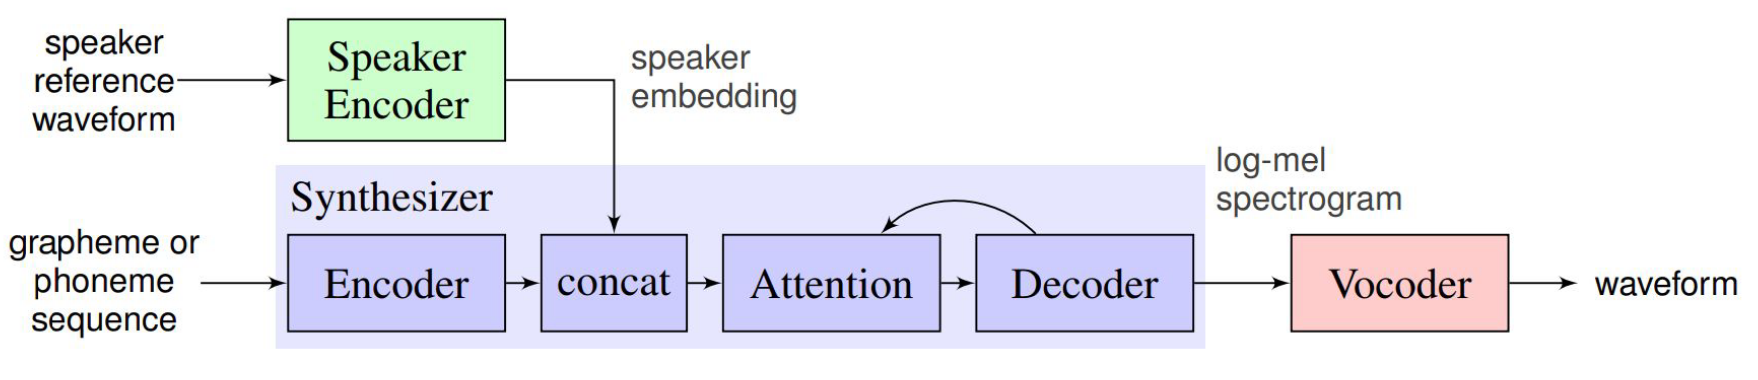
\includegraphics[width=1\textwidth]{./graphics/rtvc.png}
  \caption{RTVC Architecture \cite{jemineRealTimeVoiceCloning2019}.}
  \label{fig:rtvc-arch}
\end{figure}

The \gls{rtvc} workflow cleverly introduces a speaker encoder to the training process of the synthesizer (see Figure \ref{fig:rtvc-arch}). The speaker encoder is based on speaker verification and voice recognition and provides a speaker embedding, which can be understood as a fingerprint of a person's voice. The synthesizer is then trained with the speaker embeddings as an additional input. During inference, one must provide a speaker embedding (the reference voice sample). Based on the embedding, the synthesizer then produces the cloned voice without having been trained on the voice in advance. We experimented with the \gls{rtvc} in 2021. At the time, it only worked with English voices, nonetheless we tried to train a German model on our own. The results were unsatisfying. Today, with X-TTS, German voices do not sound good enough, which is why we switched back to the time consuming retraining approach with VITS. \\
Regarding our VITS training duration, we first trained a first run with 90 minutes of training material for two weeks on an RTX 4090 GPU. The second run, with four hours of material, was conducted on an A6000 GPU and took approximately one week until the loss values converged. 

\section{Voice-to-Voice Conversion}
\label{sec:v2v}
Besides \gls{tts}, another recently published approach was tested: \gls{v2v} conversion. The main difference to \gls{tts} is that \gls{v2v} takes actual speech as an input and outputs an audio file sounding like the targeted voice. This approach can address the problem with \gls{tts}, where the synthesized voice sounds monotonous. Because the tonality of the target speaker is retained after converting it to the other voice, an actor can influence how the result should sound. On the other hand, certain mannerisms in the actor's voice will translate the result, for example, an odd-sounding pronunciation of the letters \textit{S} or \textit{R}, hissing, or something else. Many participants also noted a strong resemblance of the converted voice to the actual speaker's voice. For accomplishing \gls{v2v} conversion, the \gls{rvc} project was used \cite{RVCProjectRetrievalbasedVoiceConversionWebUI2023}. 

\begin{figure}[h]
  \centering
  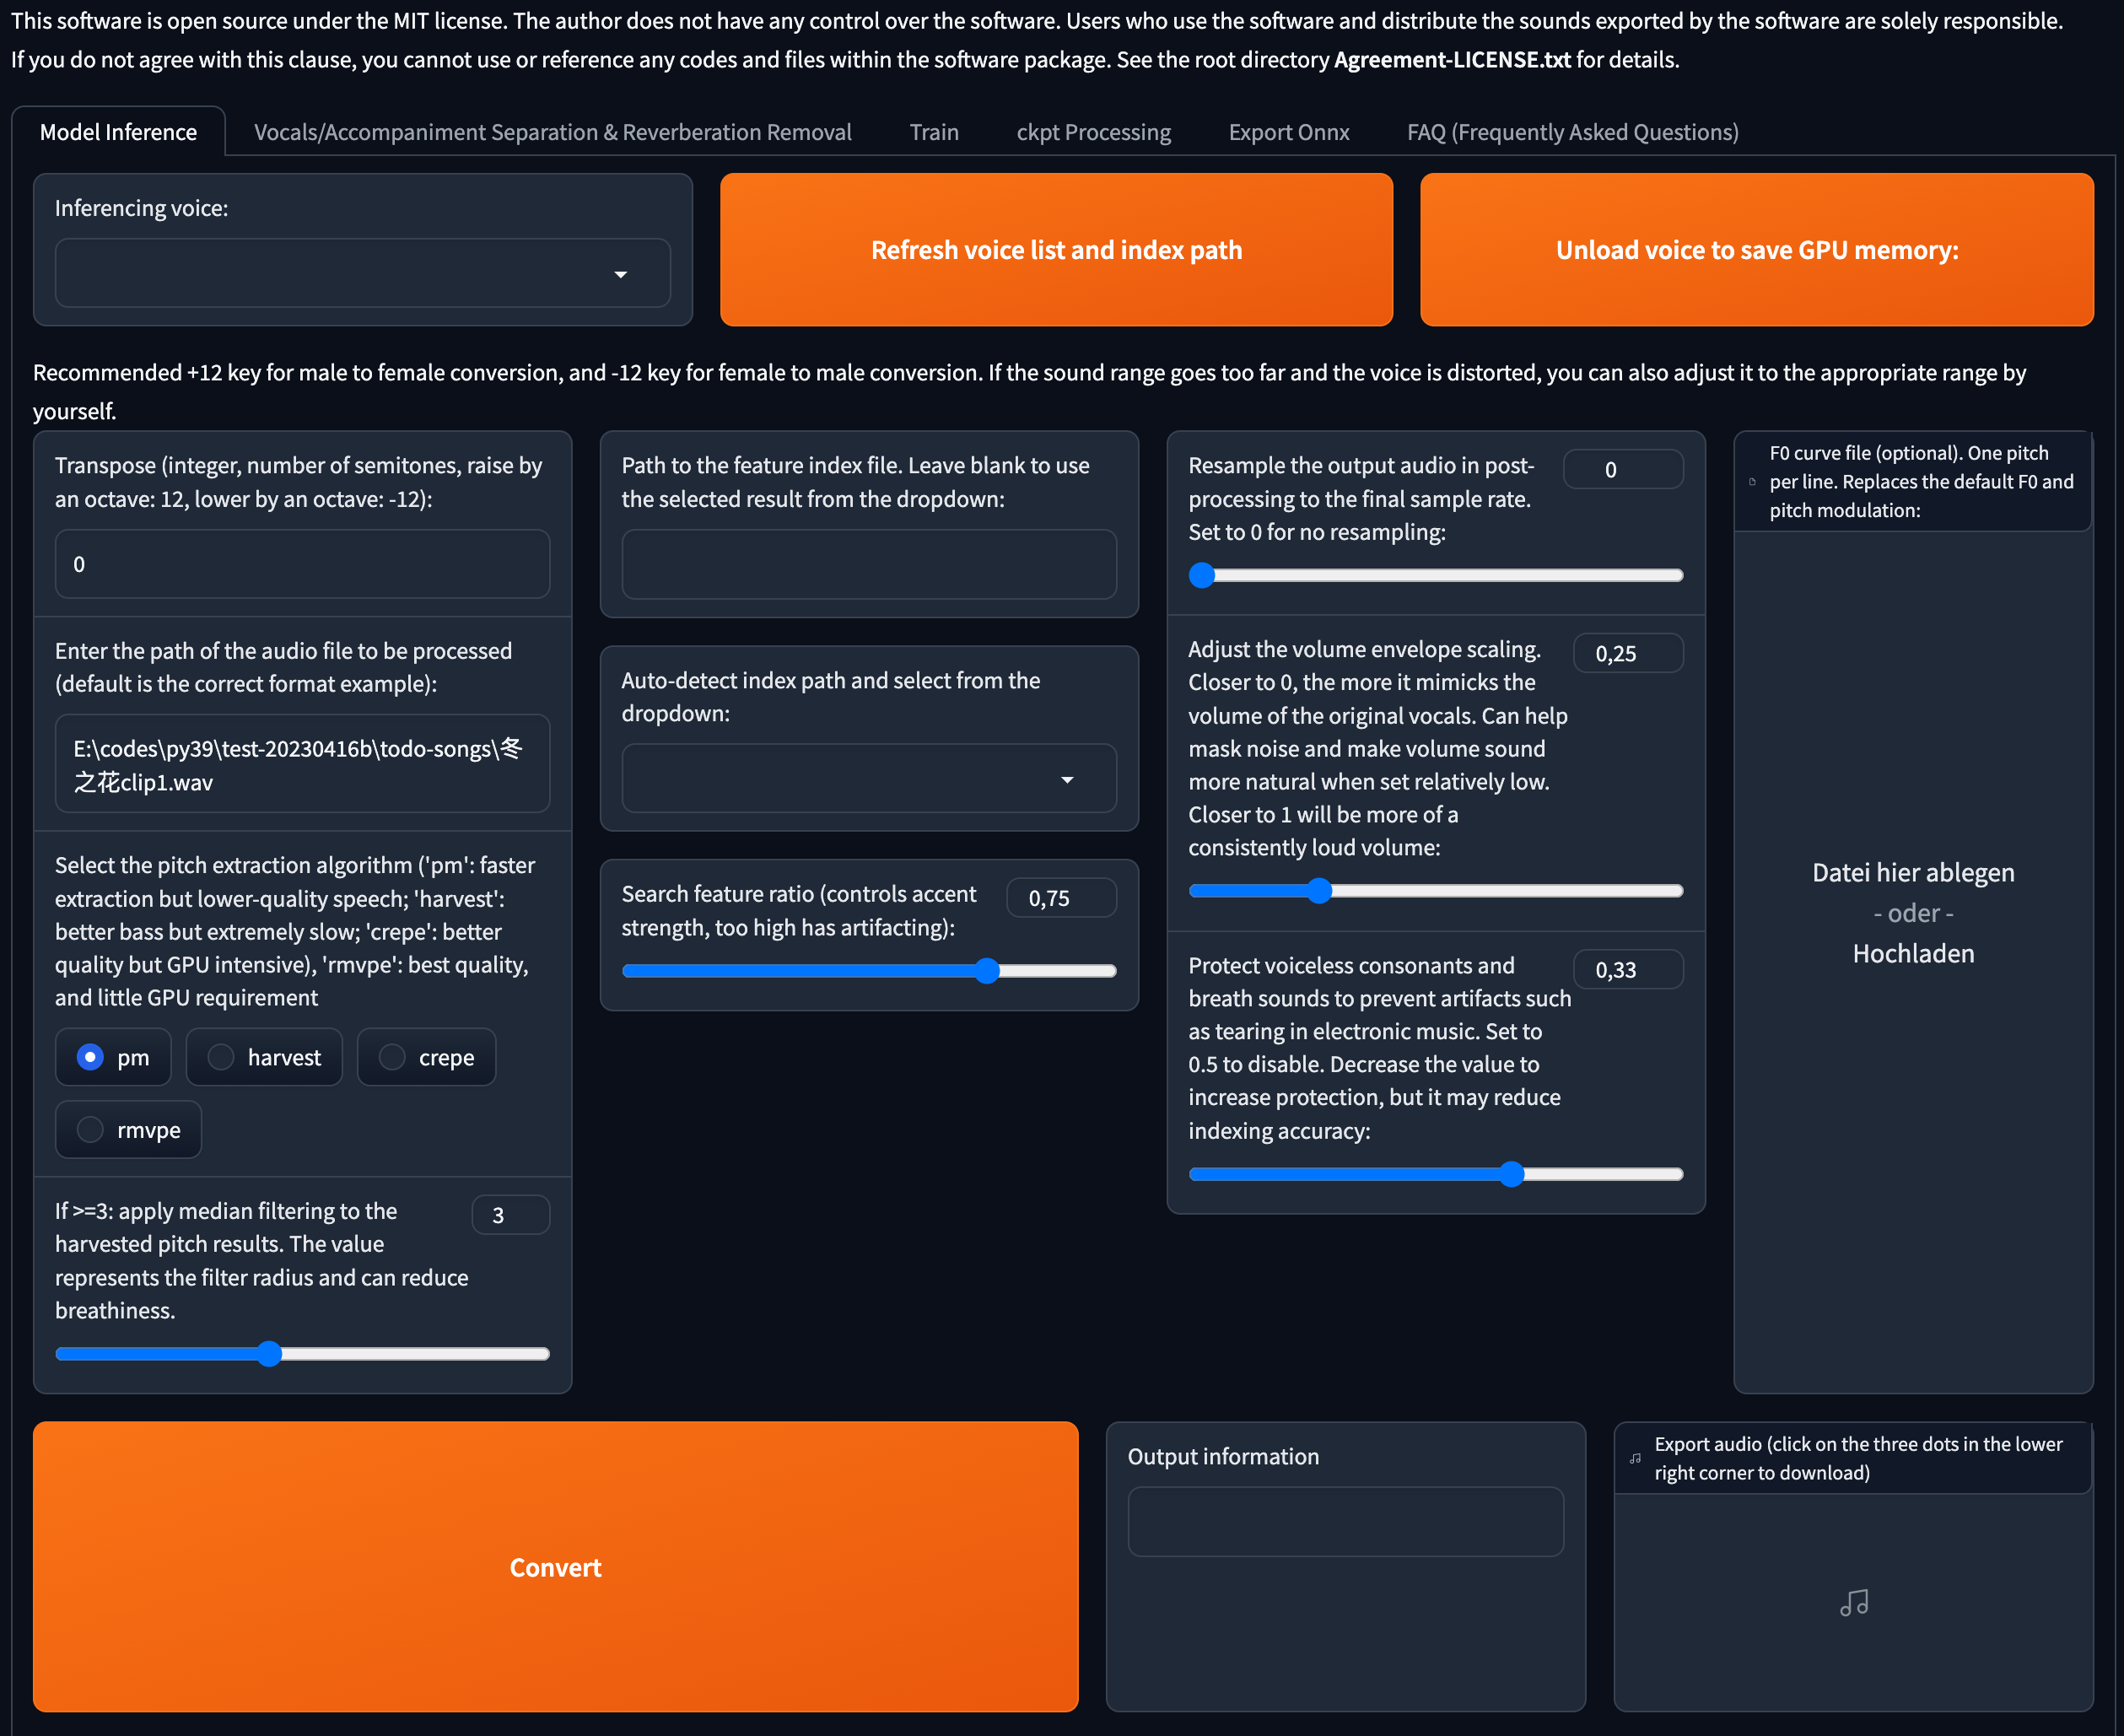
\includegraphics[width=1\textwidth]{./graphics/RVC-UI.png}
  \caption{Retrieval-Based Voice Conversion Gradio User Interface.}
  \label{fig:rvc-gradio}
\end{figure}

The project features a Gradio.io user interface (Figure \ref{fig:rvc-gradio}) for easy cloud deployment and is quite self-explanatory. Regarding the dataset requirements, approximately 10 minutes of a person's voice is required. The data preprocessing does not require any text file transcription as with \gls{tts} but does require cutting up the voice samples into sections under 10 seconds to avoid an \gls{oom} error. This can be easily achieved with the preprocessing toolkit developed for the \gls{tts} section of this work. The training itself takes approximately one hour on an A6000 GPU.

After training is completed, inferencing the model can be accomplished quickly. \gls{rvc} processes input audio files in nearly real time. It is to be noted that an actual real-time voice changer for these models has been implemented as  \cite{WokadaVoicechangerVoice}. One can use input from a file or microphone, and the voice changes with little delay (100ms on a suitable graphics card). The implications of such real-time voice-fake capabilities are interesting in the domain of deepfakes and scams. There have been some reports that fake voices have been used to conduct scams. However, these were often accomplished using \gls{tts} and preparing the sound snippets for playback. Combining such a technology with real-time face swaps shows the need for caution and multifactorial security in videocall-based social interaction. Interestingly, these voice models are shared among creators on platforms such as Civit.ai, but the technology has not yet had as much of an impact as \gls{sd}.

\gls{v2v} models could also be used to improve \gls{tts} quality in a similar fashion as suggested with \gls{w2l} and face swaps: one could train a faster but lower quality \gls{tts} model and then upsample the voice quality in realtime with \gls{v2v}. We have not conducted any experiments in this direction due to time constraints and the fact that it would have required a shift in the \gls{tts} approach.

\section{Game Engines and Virtual Production}
\label{sec:bg-virtual-production}
A few years before the big leap in \gls{genai}, virtual production methods started to gain traction within the film and broadcasting industry. Instead of filming in front of a greenscreen, the production team of \textit{The Mandalorian} (2019) famously used a large LED panel around the whole studio walls and ceiling to shoot their series (Figure \ref{fig:mando-vps}). That way, many effects could be achieved in camera as opposed to in post production, as it was usually done.

\begin{figure}[h]
  \centering
  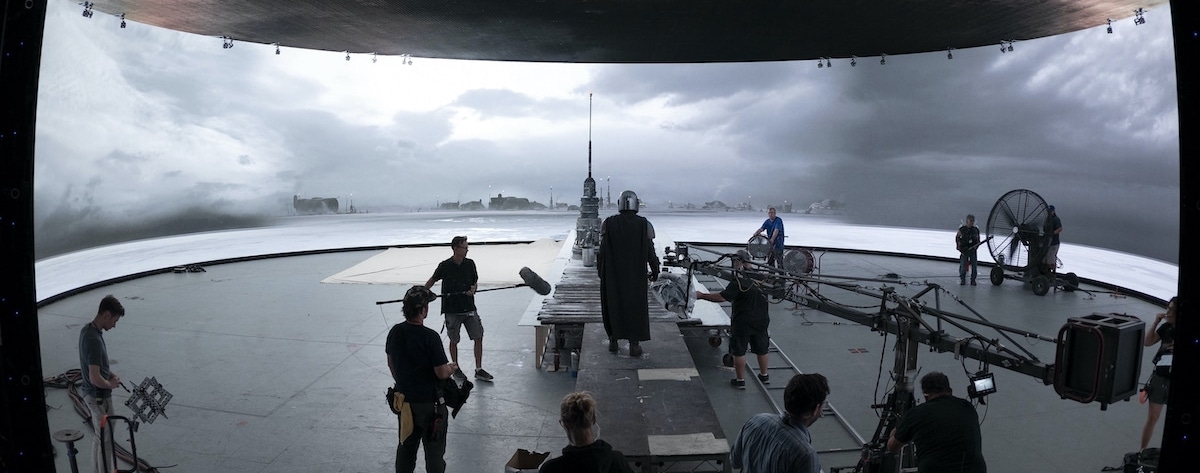
\includegraphics[width=1\textwidth]{./graphics/mandalorian-vp.jpg}
  \caption{\textit{The Mandalorian} Studio and LED-Volume "Stagecraft" \cite{landsiedelGamechanger2021}.}
  \label{fig:mando-vps}
\end{figure}

The important shift in technology consisted not only in the use of LED panels but also in what rendered the images on the screens. It is a specific kind of software, usually found in the gaming industry, called \gls{ue}, a so-called \textbf{game engine}, developed by Epic Games. The engine's capability to render photorealistic images in real time made it the ideal driver for this novel movie production. Today, \gls{ue} can be used to generate not only environments but humans as well. Epic Games' software, \textit{Metahuman Creator}, allows for easy character creation. 

\begin{figure}[h]
  \centering
  \begin{subfigure}[b]{0.45\textwidth}
    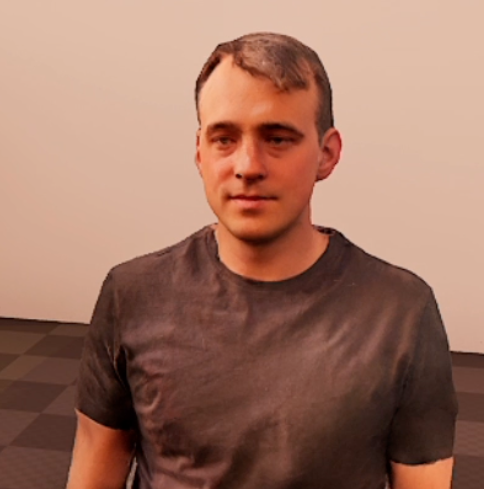
\includegraphics[width=\textwidth]{./graphics/unreal-engine/photogrammetry.png}
    \caption{Photogrammetry Scan.}
    \label{fig:head-photogrammetry-scan}
  \end{subfigure}
  \hfill
  \begin{subfigure}[b]{0.5\textwidth}
    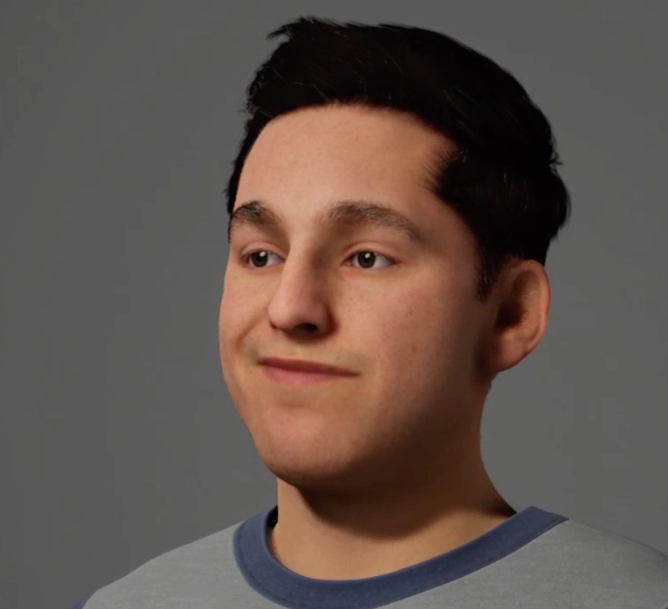
\includegraphics[width=\textwidth]{./graphics/unreal-engine/Metahuman.png}
    \caption{Metahuman based on photogrammetry Scan.}
    \label{fig:metahuman-result}
  \end{subfigure}
  \caption{Mesh to Metahuman Workflow.}
  \label{fig:metahuman-comp}
\end{figure}

It is also possible to scan a face and transfer the geometry onto a metahuman. An example of such an approach can be seen in Figure \ref{fig:metahuman-comp}, although this experiment did not work particularly well. During the timeframe of our investigations, the process for creating metahumans improved considerably. It is only a matter of time until these metahumans become more advanced. Currently, gaussian splatting seems to be a key technology to watch in this regard.

It should be noted that \gls{ue} is a complicated tool that needs a great deal of time to be mastered. In addition to \gls{ue}, many other, more specialized tools need to be used to get the best possible output. These include modeling software for environments and characters, as well as texturing tools and many more. \gls{ue}, in the end, is good at combining all the assets, but to obtain high-quality results, a team needs experts in many different areas of computer animation. It becomes quickly evident that the metahuman characters fall into the uncanny valley. Improving the face quality was explored using a \gls{dfl} model on top of the \gls{ue} rendering. Unfortunately, the uncanny part of the face is not the appearance of the face but its movements. This most likely has to do with how the face is animated. The facial performance capture is accomplished using the iPhone's FaceID camera, which has limitations in how many facial landmarks it can track, therefore limiting facial movement fidelity. Consequently, the facial movements look uncanny. These facial movements would translate directly to a potential \gls{dfl} face mask, which is why we decided not to complicate our workflow for only, if any, minor improvements.

\chapter{Related Work}
\label{chap:rel-work}
% Introduction
Chapter \ref{chap:background} served the purpose of providing some technical background and establishing a general understanding of how the used technologies can be applied. Now, we present some related work in the domain of psychological and sociological research that has been done in the context of (synthetic) media trust, credibility, and the effects of fake news in general. 

\begin{quotation}
  "We urge researchers to begin to study the social issues surrounding deepfake technology. The studies in this volume do a fantastic job of mapping out the research questions, applying theory to the phenomenon, and creating new tools to apply to future research. But this study is preliminary, and we urge scholars to build upon this study as deepfake use continues to grow." \cite[p. 151]{hancockSocialImpactDeepfakes2021}
\end{quotation}

With this call to action, \textit{Cyberpsychology, Behavior, and Social Networking} (volume 24, issue 3) published several articles that can be summarized as discussing the social impact of deepfakes. This was in 2021, three years after deepfake face swaps had become dominant and before \gls{llm}s \gls{t2i} were available. To begin with, \citet{hancockSocialImpactDeepfakes2021} raise a few questions about deepfakes: Does exposure to deepfakes undermine trust in the media? How might deepfakes be used during social interactions? Are there strategies for debunking or countering deepfakes? The authors concluded that empirical research on the social impact of deepfakes is scarce and therefore refer to neighboring fields. \\
In an introduction to the topic as a whole, \citet{hancockSocialImpactDeepfakes2021} cite studies on false memory acquisition by \citet{garryActuallyPictureWorth2005}. These experiments often involve some doctored footage of participants, often created with 3D animation tools, and prove that it is possible to induce false memories with that approach. \\
\citet{hancockSocialImpactDeepfakes2021} also mention deception research and conclude that people perform only slightly above chance when evaluating a message as either true or deceptive \cite{bondAccuracyDeceptionJudgments2006}. They state, "Studies have shown that deception detection is approximately the same whether the message is conveyed through text (e.g., a court transcript, an Internet chat log), an audio recording (e.g., a voicemail, a radio program), or a video (e.g., an interrogation video)" \cite{hancockSocialImpactDeepfakes2021}.

The references from \citet{hancockSocialImpactDeepfakes2021} show how far research in the field can reach. In the following, we will present further examples. We decided to divide the related work into four categories: In Section \ref{sec:hist-context}, we want to provide some context about the environment in which the papers were written. In Section \ref{sec:rel-secondary}, we shed some light on methods that do not address participants directly in a study but analyze secondary indicators such as newspaper articles, forum blog posts, and video comments. In Section \ref{sec:rel-studypart}, we discuss controlled studies that were conducted with individual participants who consumed some kind of synthetic content. Our own paper should fall under the latter category as well. Finally, in \ref{sec:rel-work-counteringdf}, we added some works about countering maleficent synthetic media.

\section{Historical and Socio-Geographical Context}
\label{sec:hist-context}
As stated in the introduction, synthetic media is a rather new trend, mainly driven by the advance of \gls{genai}. It can be dated back to the earliest of 2017, when deepfake face swaps surfaced in the broader public. It is remarkable that the term "fake news" is also very young, having developed about the same time as deepfake face swaps, around 2016. For completeness, it should be noted that the Merriam-Webster Dictionary dates the first use of the term "fake news" back to the year 1890 \cite{merriam-websterdictionaryRealStoryFake}. Surely skepticism has always existed towards politics and media, but it was not a significant topic until Donald Trump entered his presidential campaign in 2016, as can be seen in the Google trend analyses in Figures \ref{fig:gtrend-fake-news} and \ref{fig:trust-us}. That said, it would not make much sense to look for related work earlier than 2016–2017. Therefore, we focused our attention on the timeframe in which deepfakes came into existence and fake news became a publicly relevant topic.

\begin{figure}[h]
  \centering
  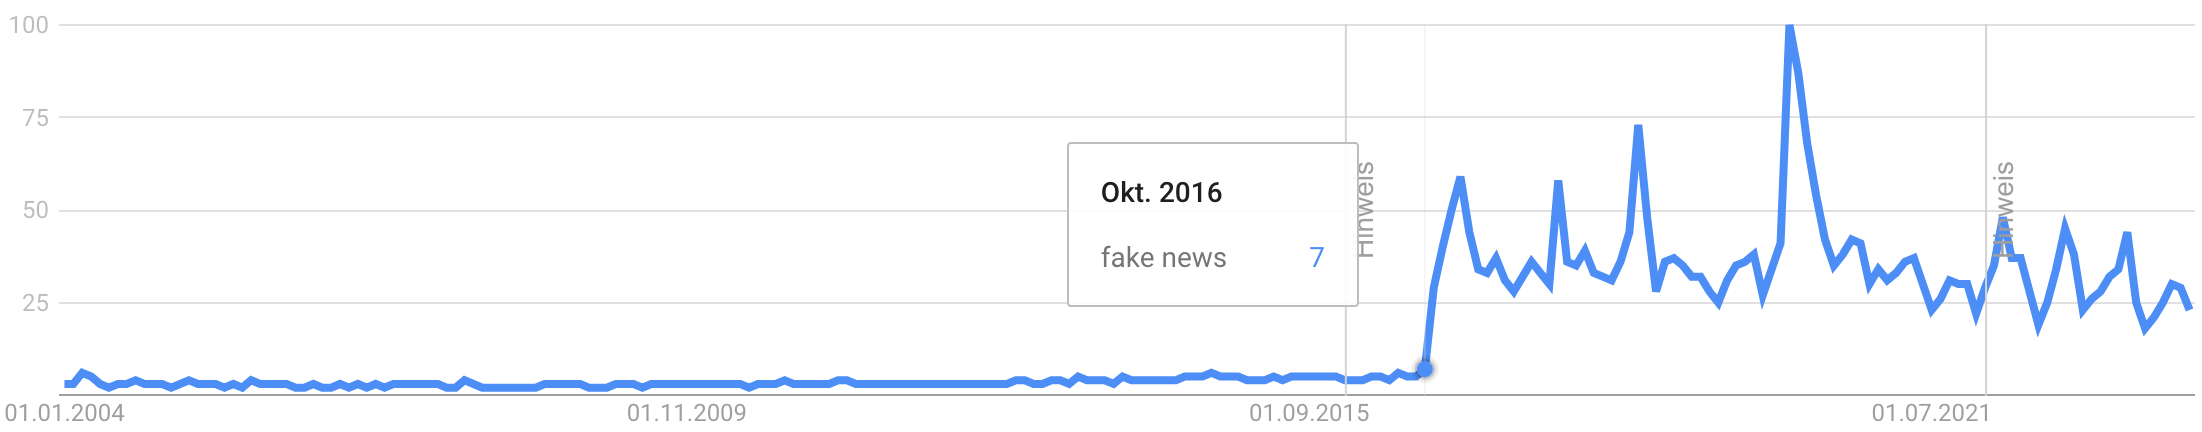
\includegraphics[width=1\textwidth]{./graphics/gtrends_fakenews_1011-2311.png}
  \caption{Google Trends of the Term "Fake News" 2004–2023.}
  \label{fig:gtrend-fake-news}
\end{figure}

In our study, we investigate a German-speaking population. Therefore, we want to remark that most papers that are focused on a certain territory (mostly US in relation to Trump) can only be included, with the caveat that some research might not directly apply to the German cultural space as well. To illustrate one difference, we can refer to Figure \ref{fig:trust-ger} in comparison to Figure \ref{fig:trust-us}. While trust in the news media among the American public decreased around 2016, no impact was seen in Germany at this time. It took until the years of the COVID-19 pandemic to experience a decline in Germany as well. It remains to be seen how this trend will continue in the following years.

\begin{figure}[h]
  \centering
  \centering
  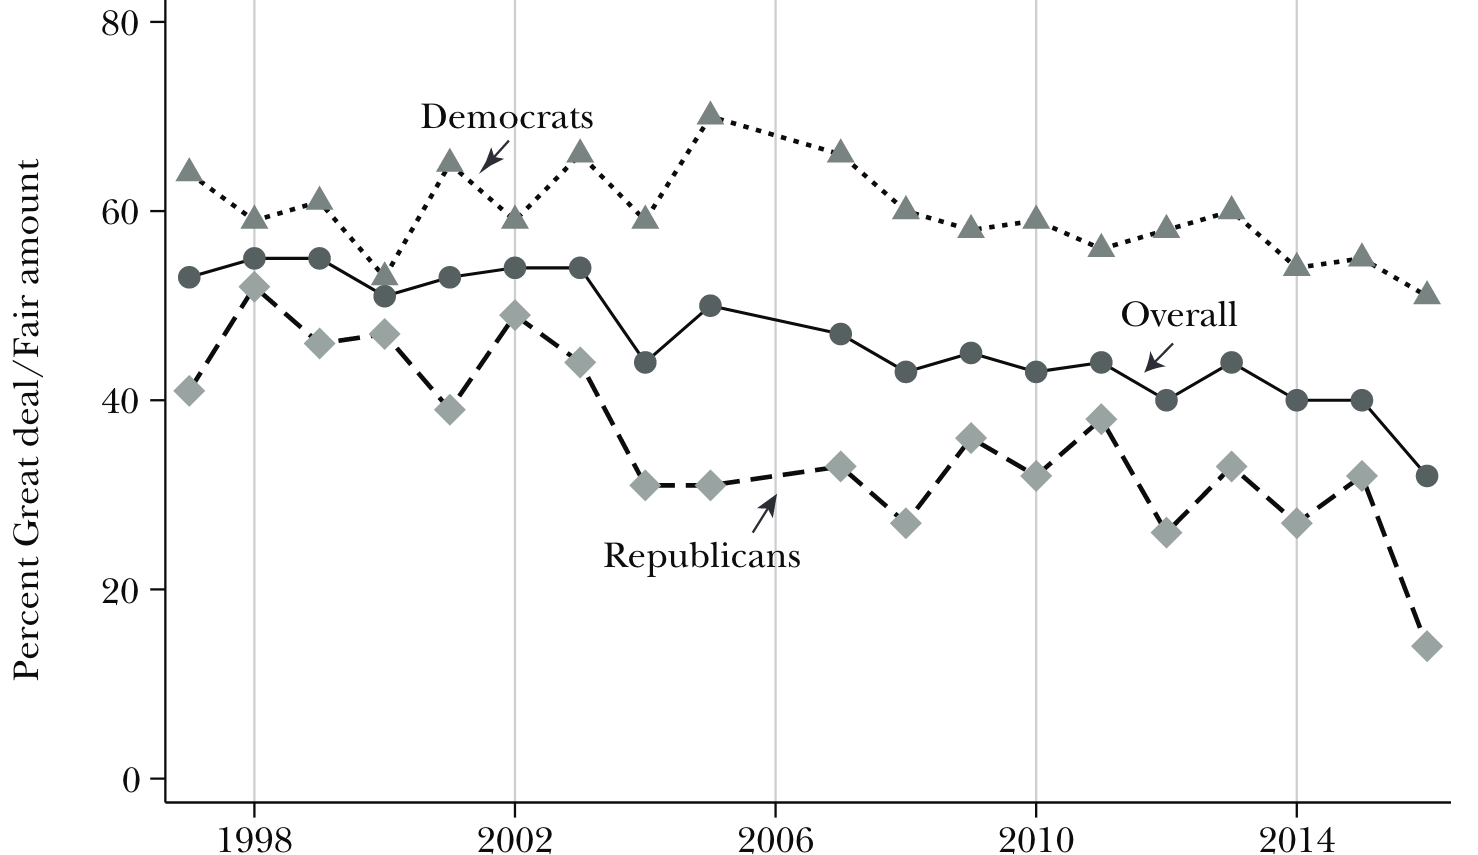
\includegraphics[width=0.75\linewidth]{./graphics/trust-america mainstream.png}
  \caption{Trust in American Mainstream Media 1996–2017 \cite{allcottSocialMediaFake2017}.}
  \label{fig:trust-us}
\end{figure}
\begin{figure}[h]
  \centering
  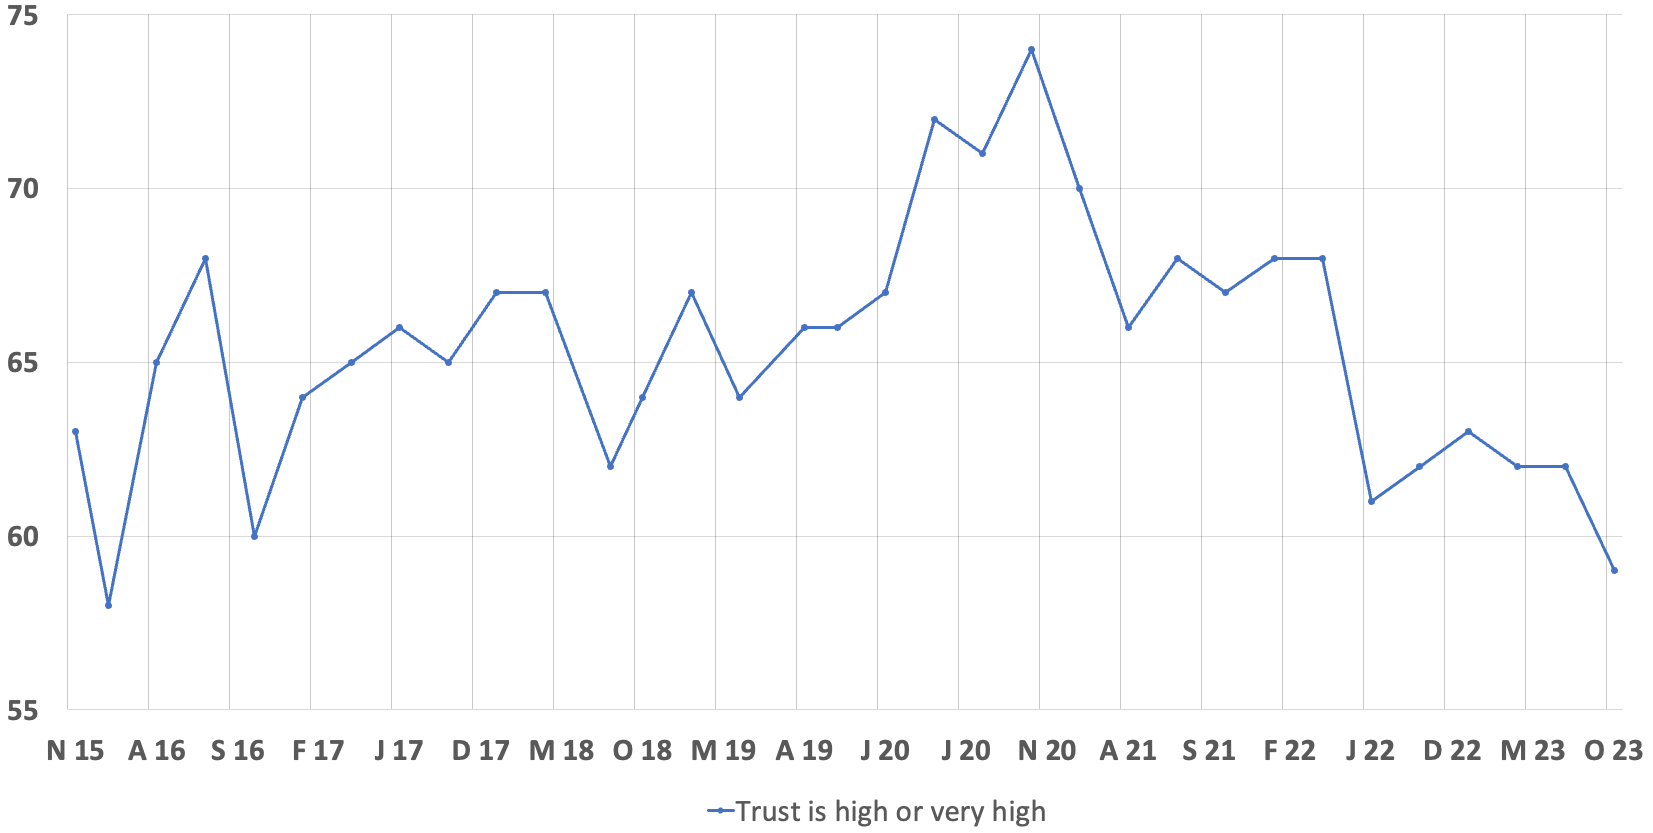
\includegraphics[width=0.8\linewidth]{./graphics/FGW-Trust-in-ARDZDF.png}
  \caption{Question: How high is your trust in \gls{psm}, ARD, and ZDF? (2015–2023) \cite{zdf-politbarometerVertrauenGlaubwuerdigkeitBerichterstattung2023}.}
  \label{fig:trust-ger}
\end{figure}

Surely, it is impossible to pinpoint one singular event, person, or technology as the starting point for trust issues within a society. We chose to present this research from a technological perspective, and while we define deepfakes as the umbrella term for all synthetically generated fake news, we will chronologically encounter face swaps first, as they are the oldest (2017) of the relevant technologies. The next deepfake tool to come around was probably Wav2Lip in 2020. Please bear in mind that literature published before the \gls{genai} boom of 2022 refers to deepfake face swaps in most cases, simply because other technologies were nonexistent or irrelevant to the public until very recently. The term "deepfake" was often used analogously with face swaps until other technologies advanced, such as synthetic voices, lip remapping, and today's image generators.

\section{Perceptions and Implications Through Secondary Indicators} 
\label{sec:rel-secondary}

Investigating deepfake technology through secondary indicators, such as video comments or blog posts, is essential to comprehensively grasping public sentiment and articulating feelings surrounding this technological advancement. Analyzing these sources provides valuable insights into how individuals perceive and express their concerns, contributing to a nuanced understanding of the societal implications of deepfake technology. By looking into the diverse array of opinions presented in video comments and blog posts, we gain a more holistic view of the multifaceted landscape surrounding deepfakes.

\subsubsection*{News Article Reviews}
Mika \citeauthor{westerlundEmergenceDeepfakeTechnology2019a} provides a literature review on emerging scholarly literature in addition to publicly available news articles. The researcher uses this data to reflect on the benefits, threats, and examples of current fakes and how to combat them. \citeauthor{westerlundEmergenceDeepfakeTechnology2019a} lists several benefits in the regions of media production, educational media and digital communications, games and entertainment, social media and healthcare, material science, and various business fields, such as fashion and e-commerce. As examples, \citeauthor{westerlundEmergenceDeepfakeTechnology2019a} names several entertaining deepfakes of famous actors and a museum installation that brought Salvador Dalì back to life. The author also concludes, "According to our study, deepfakes are a major threat to society, the political system and businesses" \cite[p. 47]{westerlundEmergenceDeepfakeTechnology2019a}. The author reached this conclusion based on the existence of countless pornographic deepfakes, and multiple political fakes. The Obama/Peele fake is quoted again, along with a viral video of the American politician Nancy Pelosi and another fake of Donald Trump. The authors evaluated these videos as having limited political influence, but they also provide two examples where fakes had consequences. In one case from 2018, a deepfake of Gabon's long-unseen president, Ali Bongo, who was believed to be in poor health or dead, was cited as the trigger for an unsuccessful coup by the Gabonese military. In the other case, a viral clip from Malaysia showed a man's confession of having had sex with a local cabinet minister, which caused political controversy.

Regarding a possible solution, \Citeauthor[p. 47]{westerlundEmergenceDeepfakeTechnology2019a} names four fields of action: "1) legislation and regulation, 2) corporate policies and voluntary action, 3) education and training, and 4) anti-Deepfake technology." Section \ref{sec:rel-work-counteringdf} gives further insight into some countermeasures.

\subsubsection*{YouTube Comment Analysis}
The works of \citeauthor{leeBelieveNotBelieve2021} take a different approach and move closer to the corupus delicti. They picked the top 10 deepfake videos on YouTube and provided a framing analysis of the audience's comments. The word "framing" is important here and requires an explanation. Framing refers to how a certain piece of information is contextualized, or, in the words of the authors, "The \textit{valence framing} effect explores how information, framed positively or negatively, may systematically affect audience responses" \cite[p. 153]{leeBelieveNotBelieve2021}. From the 10 most-viewed deepfake YouTube videos, the authors gathered 88,362 comments, from which they chose 2,689 (3\%) randomly sampled comments for further analysis. They then analyzed how the videos were framed and looked at the framing of the comments.\\
Five videos were positively framed; three were classified as neutral, and two had negative framing. Regarding the comments, the authors found that there were quite distinct groups who recognized positive or negative potential for deepfakes but rarely saw both a positive and negative side to the technology. These distinct groups were also in line with the framing of the corresponding videos. The authors conclude that the audience is largely influenced by the framing of the video and remark that this situation might not be ideal for the education of all viewers, as the opposite opinion is always missing. This is quite an easy argument to follow. Of course, more shades of grey are always better for a balanced discourse. However, we have to consider doubts about the depth of information one can extract from these comments. We assume that a video comment is rarely a detailed, dialectic thought but more of a spontaneous reaction to the seen video. That said, it seems difficult to make a conclusive assessment of the viewers' thoughts. Nonetheless, the findings remain interesting and show that a balanced coverage of such a delicate topic is important.

\subsubsection*{Reddit Sentiment Analysis}
Similar to the works of \citeauthor{leeBelieveNotBelieve2021}, \citeauthor{brooksPopularDiscourseDeepfakes2021} qualitatively investigated the framing of deepfakes but instead used posts from the platform Reddit. It is still quite interesting because \citeauthor{brooksPopularDiscourseDeepfakes2021} chose posts from December 2017 to February 2018, which is exactly the timeframe and platform when and where deepfake pornography emerged. During the analysis, two primary topics emerge: (1) risk to individuals by way of personal abuse and reputation decimation, and (2) risk to society in terms of war threat and societal impact. As an interesting sidenote, the authors mention parallels to the rise of the Internet, where similar threats are assumed. To conclude, \citeauthor{brooksPopularDiscourseDeepfakes2021} points to the need for various solutions for different problems that arise from the emergence of deepfakes. \\
According to \citeauthor{brooksPopularDiscourseDeepfakes2021}, personal responsibility and individual literacies are often proposed as solutions but fail to consider differences in culture, language, or digital literacies. The author advocates for advanced media forensics to detect fake material, a strategy that might not be sustainable in the long term, as discussed in Section \ref{sec:rel-work-counteringdf}. For instance, Brooks identifies blinking eyes as an indicator of fakes, an argument made when some deepfake face swaps showed inconsistencies in the eye area. Currently, there is a similar debate concerning \gls{sd} images, where rendered humans often have more than five fingers. It took a little time before both issues were resolved. This highlights the limitations of any automatic forensic system trained to detect deepfakes based on flawed representations. Once a flaw is identified by an automatic forensic system, it can be utilized to enhance the fake further. Ultimately, Brooks also emphasizes the need for platforms to take greater responsibility for mitigating the spread of fake news.

% Reviews with studies on actual people
\section{Controlled Studies with Participants}
\label{sec:rel-studypart}

While we have explored the broader picture using secondary indicators and public discourse, it is crucial to zoom in and examine how individuals directly respond to deepfake technology. This section shifts focus to measurements with study participants, aiming to uncover detailed insights into how deepfakes impact individuals' trust, perceptions, and behaviors and make them tangible through studies.

\subsubsection*{Vulnerability to Microtargeting}
Whether people indeed fall for deepfakes is unclear and understudied, but not unimaginable \cite{dobberMicrotargetedDeepfakesHave2021}. \citet{dobberMicrotargetedDeepfakesHave2021} particularly investigated what effect deepfakes can have when amplified through microtargeting in a fictional scenario. In a study, they interrogated 278 participants to answer the research question of how the attitudes of supporters of a depicted politician's party are affected by a deepfake video. \\
The video was meant to discredit the political candidate. As a blocking variable, they chose Christian religious identity. By answering questions about religion, the participants were placed into Christian and non-Christian groups and then randomly shown either the original video, or the deepfake video of a Dutch-Christian-Democrat politician. In the faked version, the politician jokes about Christ's crucifixion. The authors suspected that this scenario "would move attitudes because the politician is a prominent Christian politician and the base of his party is to a large extent Christian" \cite[p. 75]{dobberMicrotargetedDeepfakesHave2021} The authors found evidence that the attitude towards the politician worsened significantly in the experimental groups. Statistical evidence was also found for the hypothesis that the microtargeted Christian group was more affected by the statements than the non-Christian group.\\
All the results indicate that it is indeed possible to stage a political scandal with a deepfake. Interestingly, the findings differed from earlier authors, who found no effects of disinformation on political behavior and attitudes. They state, "indeed deepfakes are a more powerful mode of disinformation in comparison with the false news stories studied by Guess et al. (2018) and the Russian Twitter trolls studied by Bail et al. (2020)" \cite[p. 82]{dobberMicrotargetedDeepfakesHave2021}.

\subsubsection*{Sowing Uncertainty}
We have mentioned the deepfake face swap example of Barack Obama, voiced by Jordan Peele. \citeauthor{vaccariDeepfakesDisinformationExploring2020} conducted a study with exactly this material. The authors tested how a sample of 2,005 participants responded to three variants of the Obama/Peele fake. They split up the video into three separate videos. Two of them were considered deceptive because they did not include the revelation at the end, where the deepfake was explained. Of the two deceptive videos, the first one was four seconds long and included Obama "saying" that Donald Trump is a complete "dipshit". The second video was 26 seconds long and included more text. The third video contained the explanatory part of the original video, where the fake is explained and played side by side with the actor voicing Obama's image. 

The authors found that "overall, only 50.8\% of subjects were not deceived by the deepfake. This finding is surprising given the statement was highly improbable" \cite[p. 6]{vaccariDeepfakesDisinformationExploring2020}. 
It is also clear that the deception rate was quite consistent across all three videos. Much more interesting is the author's second finding: "Watching a deepfake that contains a false statement that is not revealed as false is more likely to cause uncertainty" \cite[p. 7]{vaccariDeepfakesDisinformationExploring2020}. \\
In an evaluation of the Obama/Peele fake, \citet[p. 9]{vaccariDeepfakesDisinformationExploring2020} conclude, "We have shown that political deepfakes may not necessarily deceive individuals, but they may sow uncertainty which may, in turn, reduce trust in news on social media." The authors add that these detrimental tendencies can lead to a downward spiral of trust loss in the media and news in general. This is a critical finding for all media producers and distributors, highlighting the importance of accompanying education as synthetic media proliferates. \\
In this context, it is important to add that these cases might not even need manipulated video to spread fake news and uncertainty. Text can also suffice to spread misinformation, as could be seen during the COVID-19 pandemic and the often-mentioned social media channels \cite{naeemExplorationHowFake2021}. Another example of how powerful just text alone can be is the Q-Anon conspiracy movement. \citet[p. 1]{zeeuwTracingNormieficationCrossplatform2020} investigated "how ideas and objects travel from fringe online subcultures to large audiences on mainstream platforms and news outlets." The Q-Anon subculture has led to several deaths in the real world (Pizzagate) and was related to the January 6 United States Capitol attack.

\subsubsection*{Uncanny Valley Effects}
\Citeauthor{weismanFaceUncannyEffects2021} studied the effects of 3D animated talking head avatars, specifically doppelganger recreations of the participants. These 3D characters could then be used to convey messages to their real-life counterparts. The messages consisted of one pro- and one anti-AI statement recorded from the corresponding participant in advance. Using the participants' own voices, the avatar was both voiced and animated. The animation was accomplished using the software Reallusion CrazyTalk8. Two example avatars are depicted in Figure \ref{fig:uncanny-avatars}.

\begin{figure}[h]
  \centering
  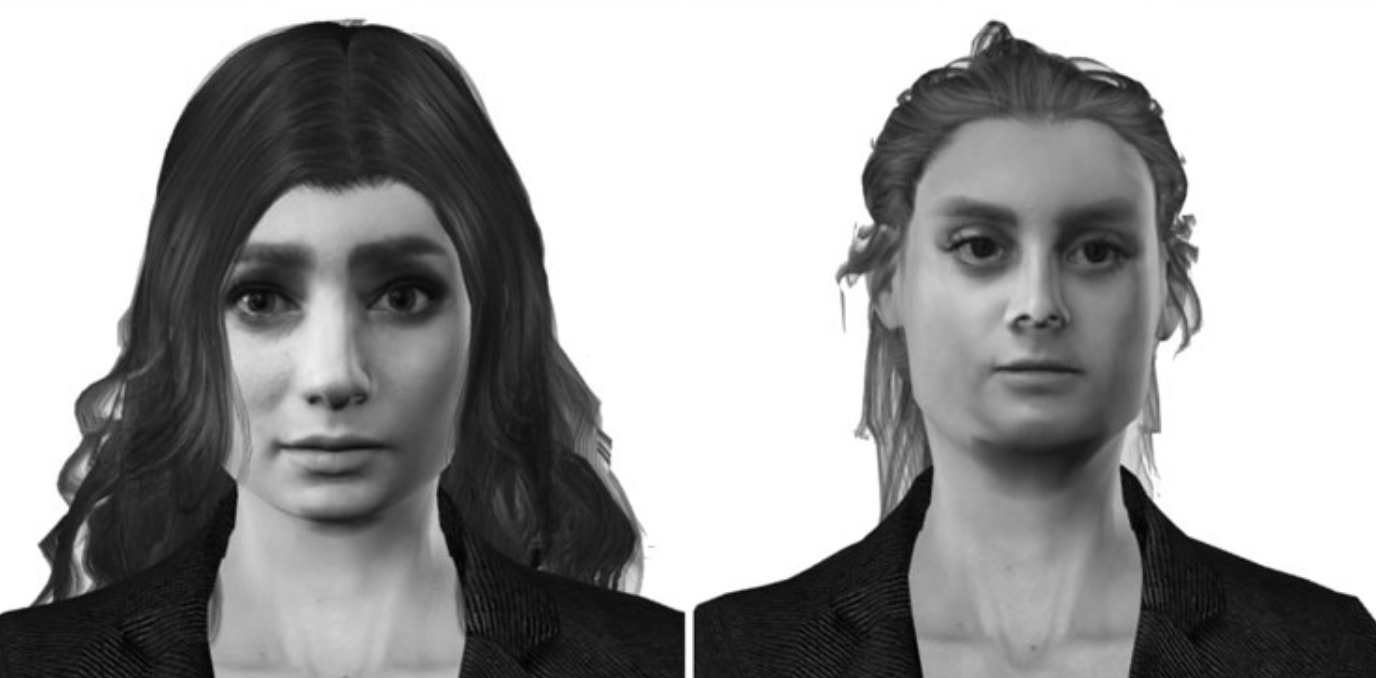
\includegraphics[width=0.75\textwidth]{./graphics/uncanny-avatars.png}
  \caption{Doppelganger Avatars Created with CrazyTalk8 \cite{weismanFaceUncannyEffects2021}.}
  \label{fig:uncanny-avatars}
\end{figure}

CrazyTalk8 uses an algorithmic approach to moving the target's head and lips based on audio; however, it is not disclosed how exactly the process works. It is imaginable that the discrepancy between the participant's natural and real voice and the rather imperfect-looking and animated 3D character induces a significant amount of uncanny valley discomfort. This is amplified as the doppelgangers portray the participants themselves, an appearance that is very familiar. The authors willingly produced a highly uncanny perception in order to measure the trust loss due to the uncanny appearance. In the study, some participants were exposed to their own voice and avatar (doppelganger), as well as another avatar and voice that were unfamiliar to them. That way, the researchers could dial the uncanny valley feeling up and down. It was higher if the participant was subjected to their own doppelganger and lower if it was a different person.\\
The authors concluded that the uncanny valley effect mediated participant-affect-based AI trust. Uncanny valley perceptions were negatively related to affect-based trust: "Presenting individuals with a talking head featuring their own face decreased affect-based trust toward AIs relative to talking heads featuring a stranger's face or relative to simple audio playback" \cite[p. 185]{weismanFaceUncannyEffects2021}.

Different from our approach, we want to remark that the study by \Citeauthor{weismanFaceUncannyEffects2021} is not suited to measure trust issues caused by artificial intelligence technology accurately, as there is no real control group that uses real footage or better AI technology (with or without uncanny valley). We can infer that the reduced trust is caused predominantly by the uncanny valley effect and not by the fact that it was created by AI-aided algorithms. We tried to address this study design difficulty by including real, non-fake material in order to receive a baseline measurement of trust for real footage, free of any \gls{genai}.

\subsubsection*{Trust in synthetic Voices}
So far, we have discussed papers that study the visual aspect of deepfakes. As explained earlier, this is most likely linked to the unavailability of easy-to-use, high-quality audio voice clones. In recent times, this has changed. Several easy-to-use \gls{tts} services can be found on the Internet. \Citeauthor{heiselbergAutomatedNewsReading2022} provide recent research about synthetic voices, or what they call "neural voices". They provide a concise summary of their findings: 

\begin{quotation}
"Results show that the participants divide into two types: the perspicacious listeners who realize or suspect that the news reading is artificially synthesized and, to some degree, are annoyed by it, and the oblivious listeners who believe the news is read by a human and are predominantly positive towards it. Participants from both groups pay particular attention to voice emotionality when evaluating the appropriateness of the neural news reader. Also, they tend to attribute human characteristics to the neural news reader. The participants single out the news messages as well as the media organization behind the news broadcast, rather than the neural voice itself, as critical components constituting credibility. Transparency is of great importance when applying a neural voice in a news broadcast, since it is a prerequisite for credibility" \cite[p. 1]{heiselbergAutomatedNewsReading2022}.
\end{quotation} 

For our work, this is especially relevant, as it is set up in the environment of a news broadcast as well. In contrast to our study, the authors focused on radio and the voice component alone. This reduced the surface area of where the uncanny valley could come into effect, thus our work, dealing with audio \textit{and} video, has to take these effects much more into account. Another difference to our work lies in the fact, that the authors conducted qualitative interviews instead of a quantitative analysis. To somewhat include a qualitative dimension as well, we gave our participants the option to justify their answers in free-text forms. 

\subsubsection*{The Disclosure of AI Reduces Trust}
As probably the most recent paper, we include \citetitle{toffTheyCouldJust2023} by \citeauthor{toffTheyCouldJust2023}. At the time of writing (December 2023) the cited paper has just been released as a preprint and has not yet been peer reviewed. The authors conducted a study using actual AI-generated journalistic content. Their focus lay on the effect of labelling AI-generated content. The studied sample consisted of audiences in the US and differed between polarized partisan lines. They found that, on average, audiences perceived news labeled as AI-generated as less trustworthy, not more (see Figure \ref{fig:toff-trust}). 

\begin{figure}[h]
  \centering
  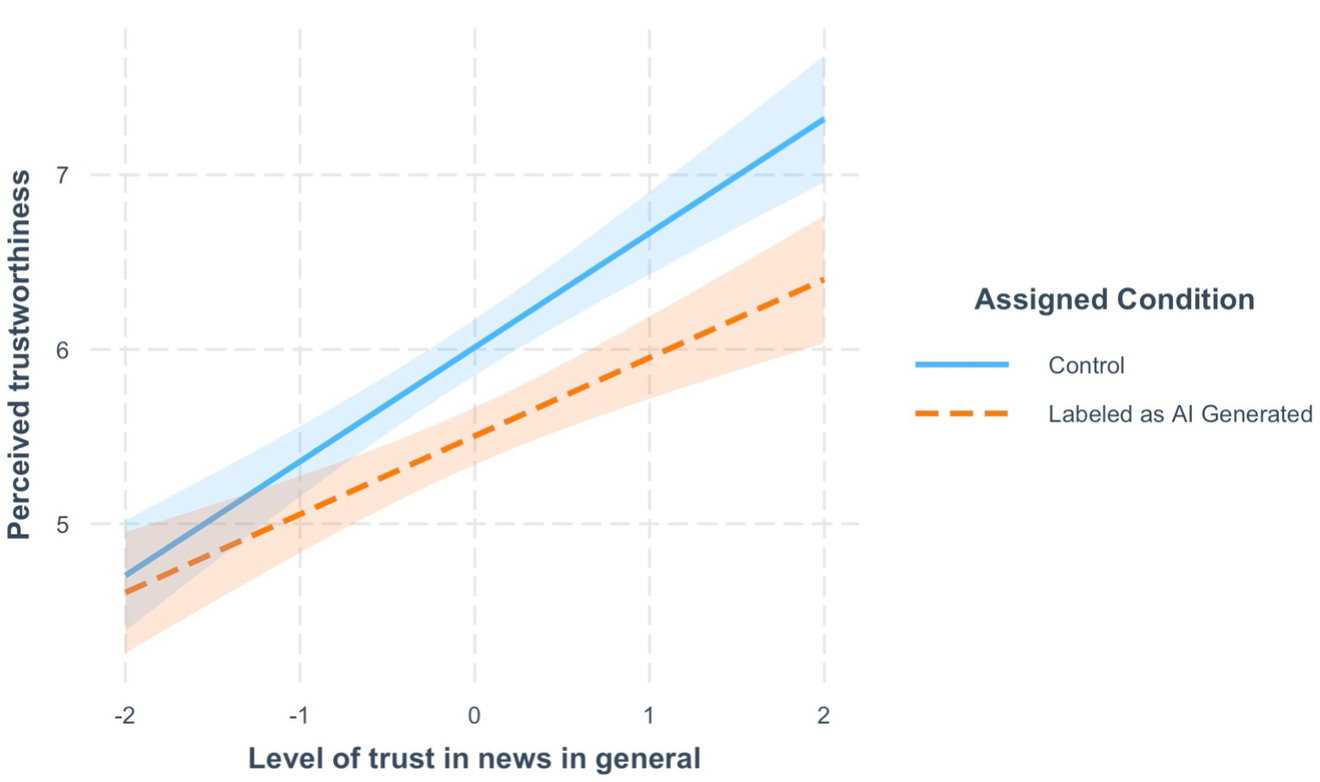
\includegraphics[width=0.8\textwidth]{./graphics/toff/Trust in news.png}
  \caption{Gaps in perceived trustworthiness associated with disclosure of the use of generative AI varied as a function of prior levels of trust in news, holding all other variables at their mean values \cite{toffTheyCouldJust2023}.}
  \label{fig:toff-trust}
\end{figure}

Furthermore, they found that these effects were largely concentrated among those whose preexisting levels of trust in news were higher to begin with and among those who exhibit higher levels of knowledge about journalism (referred to as \gls{pnk}), as depicted in Figure \ref{fig:toff-PNK}.

\begin{figure}[h]
  \centering
  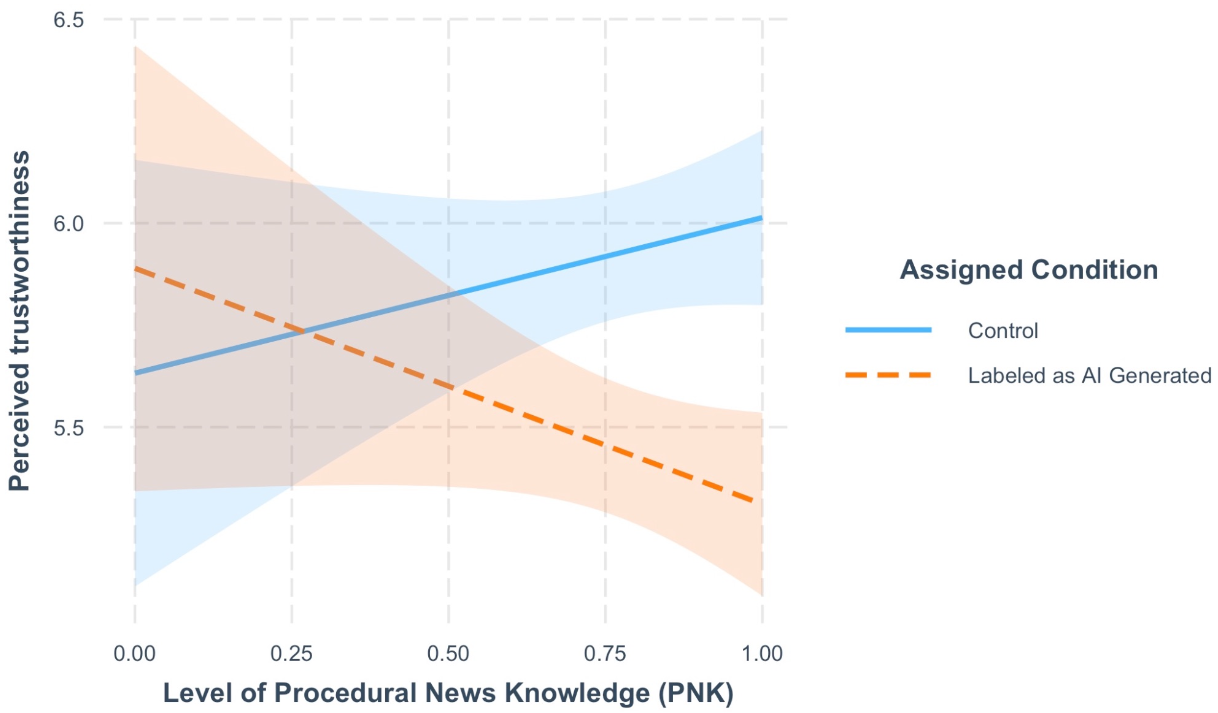
\includegraphics[width=0.8\textwidth]{./graphics/toff/PNK.png}
  \caption{Gaps in perceived trustworthiness associated with disclosure of the use of generative AI varied as a function of procedural news knowledge (PNK), holding all other variables at their mean values \cite{toffTheyCouldJust2023}.}
  \label{fig:toff-PNK}
\end{figure}

\citeauthor{toffTheyCouldJust2023} also found that the negative effects associated with perceived trustworthiness are largely counteracted when articles disclose the list of sources used to generate the content.
In contrast to our work, \citeauthor{toffTheyCouldJust2023} used AI-generated text as the object of investigation. We used AI to aid the production side of how the content was conveyed, not the content itself. Regarding our study, we could neither confirm nor disprove the results of \citet{toffTheyCouldJust2023}. Possible reasons are discussed in Section \ref{sec:results}.

\section{Countermeasures}
\label{sec:rel-work-counteringdf}
\subsubsection*{Forensic Detection is Not Sufficient}
As soon as we encounter negative use cases of synthetic media, the call for efficient countermeasures arises. Since we are dealing with deep learning techniques, a frequent suggestion is to counter fire with fire and use deep learning to train a synthetic media detector. As we mentioned earlier, anti-deepfake technology, like forensics and AI-based detection, will always have its boundaries. The efficacy will always depend on its technology's ability to detect flaws. With better detection come better methods for generation. It is an arms race that improves both parties and initially gave \gls{gan}s their name.

Because of this, other solutions in the domain of \textbf{media provenance} could provide more safety than forensic detection. In this context, Project Origin must be mentioned; It is an alliance of media producers and broadcasters who want to develop a "technical provenance approach, in conjunction with media education and synthetic media detection techniques [and] help to establish a foundation for trust in media" \cite{ProjectOrigin}. The alliance includes organizations such as the BBC, Radio Canada, The New York Times and Microsoft. This led to the creation of the \gls{c2pa}, the formulation of a technical standard to achieve the goals outlined earlier. This project is today backed by major hardware (Canon, Nikon, Sony, Leica, Panasonic, ARM) and software companies (Adobe, Microsoft, Google, AWS, AVID), media resellers, distributors, and providers (BBC, Radio Canada, dpa, france-tv, shutterstock, universal music. Clearly, \gls{c2pa} is currently being implemented by the industry.

All in all, technical solutions can only contribute a minor part to solving the problem of fake news with synthetic media. The following authors have conducted research in these areas and provide alternatives to merely technical solutions. 

\subsubsection*{The Positive Effect of Media Literacy}
\citeauthor{hwangEffectsDisinformationUsing2021} investigated the protective effect of media literacy education in the context of deepfakes. We have to point out that the authors use the term "deepfake" frequently in their paper, but it seems that their understanding of deepfakes is somewhat analogous to fake news. After all, they never mention deepfakes in the context of artificial intelligence, which contributes to our understanding of their interpretation. Neither does their study use any sort of AI-generated content but rather exposes the participants to fake news in textual form. Prior to the test, participants received two types of education: general education about disinformation and deepfake-specific education. A control group, which received no education, was also included. Adding to previous, work this study highlights the importance of the public's education in this field.

While our study did not explicitly collect any data about media literacy to use it as a dependent variable, we tried to infer such preconditions via age and occupation. Comparing \citeauthor{hwangEffectsDisinformationUsing2021}s results with our findings, we could not find any indications of an influential effect. This was most likely due to other stronger factors, underscoring the need for an isolated study on this topic.

\subsubsection*{The Positive Effect of Priming}
Related to deepfake face swaps is a study by \citeauthor{iacobucciDeepfakesUnmaskedEffects2021}, where they tried to measure the effects of information priming and bullshit (BS) receptivity on deepfake recognition and resulting sharing intention. Information priming in this context is defined as "an improvement in performance in a perceptual or cognitive task, relative to an appropriate baseline, produced by context or prior experience" \cite[p. 195]{iacobucciDeepfakesUnmaskedEffects2021}. Priming serves the purpose of increasing awareness about certain topics and therefore can be understood in a similar manner as the media literacy suggestions of \citeauthor{hwangEffectsDisinformationUsing2021}. \\
The amount of priming is measured against the participants' ability to recognize deepfakes (DF recognition). This was gauged by asking the participants if they agreed with the following statement: "The similarity of the remake to the original scene is due to the actor's abilities and not to digital video editing technologies" \cite[p. 197]{iacobucciDeepfakesUnmaskedEffects2021}. In addition to DF recognition, the authors also determined a BS receptivity index for each participant. This index was measured according to \cite{pennycookReceptionDetectionPseudoprofound2015}: Participants were asked to rate the profoundness of pseudo-profound sentences on a five-point scale from 1 = not at all profound to 5 = very profound (Examples: "Your teacher can open the door, but you must enter by yourself"; "A river cuts through a rock not because of its power but because of its persistence") \cite[p. 197]{iacobucciDeepfakesUnmaskedEffects2021}. Higher scores hint towards an inability to detect pseudo-profound statements. Based on participants' BS receptivity and DF recognition, the authors surveyed the measurements before and after priming.

\citeauthor{iacobucciDeepfakesUnmaskedEffects2021} summarize their results in two ways: (1) Participants in the priming condition showed greater DF recognition than the participants in the control condition. (2) Priming users with DF knowledge influences their ability to recognize a DF, but only when they are not strongly inclined to the reception of BS. Their hypothesis about reduced sharing intention could also be confirmed as higher levels of DF recognition (induced through priming) reduce intention to share the video through attitudes toward the video:

\begin{quotation}
"Results indicate that the development of strategies to counter the deceitfulness of DFs from an educational and cultural perspective might work well, but only for people with a lower susceptibility to believe willfully misleading claims. Finally, through a serial mediation analysis, we show that DF recognition does, in turn, negatively impact users' sharing intentions, thus limiting the potential harm of DFs at the very root of one of their strengths: virality. We discuss the implications of our finding that society's defense against DFs could benefit from a simple, reasoned digital literacy intervention" \cite[p. 194]{iacobucciDeepfakesUnmaskedEffects2021}.
\end{quotation}

The listed methods all provide some degree of mitigation to the deepfake problem on an individual level. At the size of a society, laws and policies should help as well. Unlike public opinion, there are already laws in place that should provide societal protection from both personal harm and disinformation tactics. Defamation, infringements of one's own image, privacy intrusion – these are all offenses not exclusive to synthetic media misuse. Therefore, no specific AI act is needed to counter misuse. Because of this, we did not research lawmaking literature in this context, as it has already been extensively studied in other domains. The missing component to counter the threats might be the consequent enforcement of the existing laws in virtual space. 

\subsubsection*{Literature Conclusion}
We have listed several studies about the effects of some forms of synthetic media. Regarding mitigation at the individual level, education, increasing media, and deepfake literacy are efficient ways to reduce threats from deepfakes. Overall, we realized that the available literature rarely covers newer forms of \gls{genai}. \\
We conclude that research involving \gls{genai}-created media is still scarce. This is logical due to the novelty of the technologies, their complexity, and the availability of tools for creation. These technologies are advancing at such a rate that it is impossible to keep all developments in sight. Research has just caught up with the outcome of face swap deepfakes, which today look antiquated in the light of ChatGPT and \gls{sd}. It is obvious that the research community has to continue to follow the call from \citet{hancockSocialImpactDeepfakes2021} for study.

\chapter{Implemented Technologies}
\label{chap:implementation}
Having established a theoretical background as well as an overview of existing works, we will now move on to the means we used to conduct our studies. Starting with a description of the technical implementation, we will follow with the actual study. In order to better understand why we chose certain technologies, we want to elaborate on one central thought in our work: the spectrum of artificiality depicted in Figure \ref{fig:spectrum}.\footnote{A detailed video description is provided in Table \ref{tab:video-table}.}

\begin{figure}[h]
  \centering
  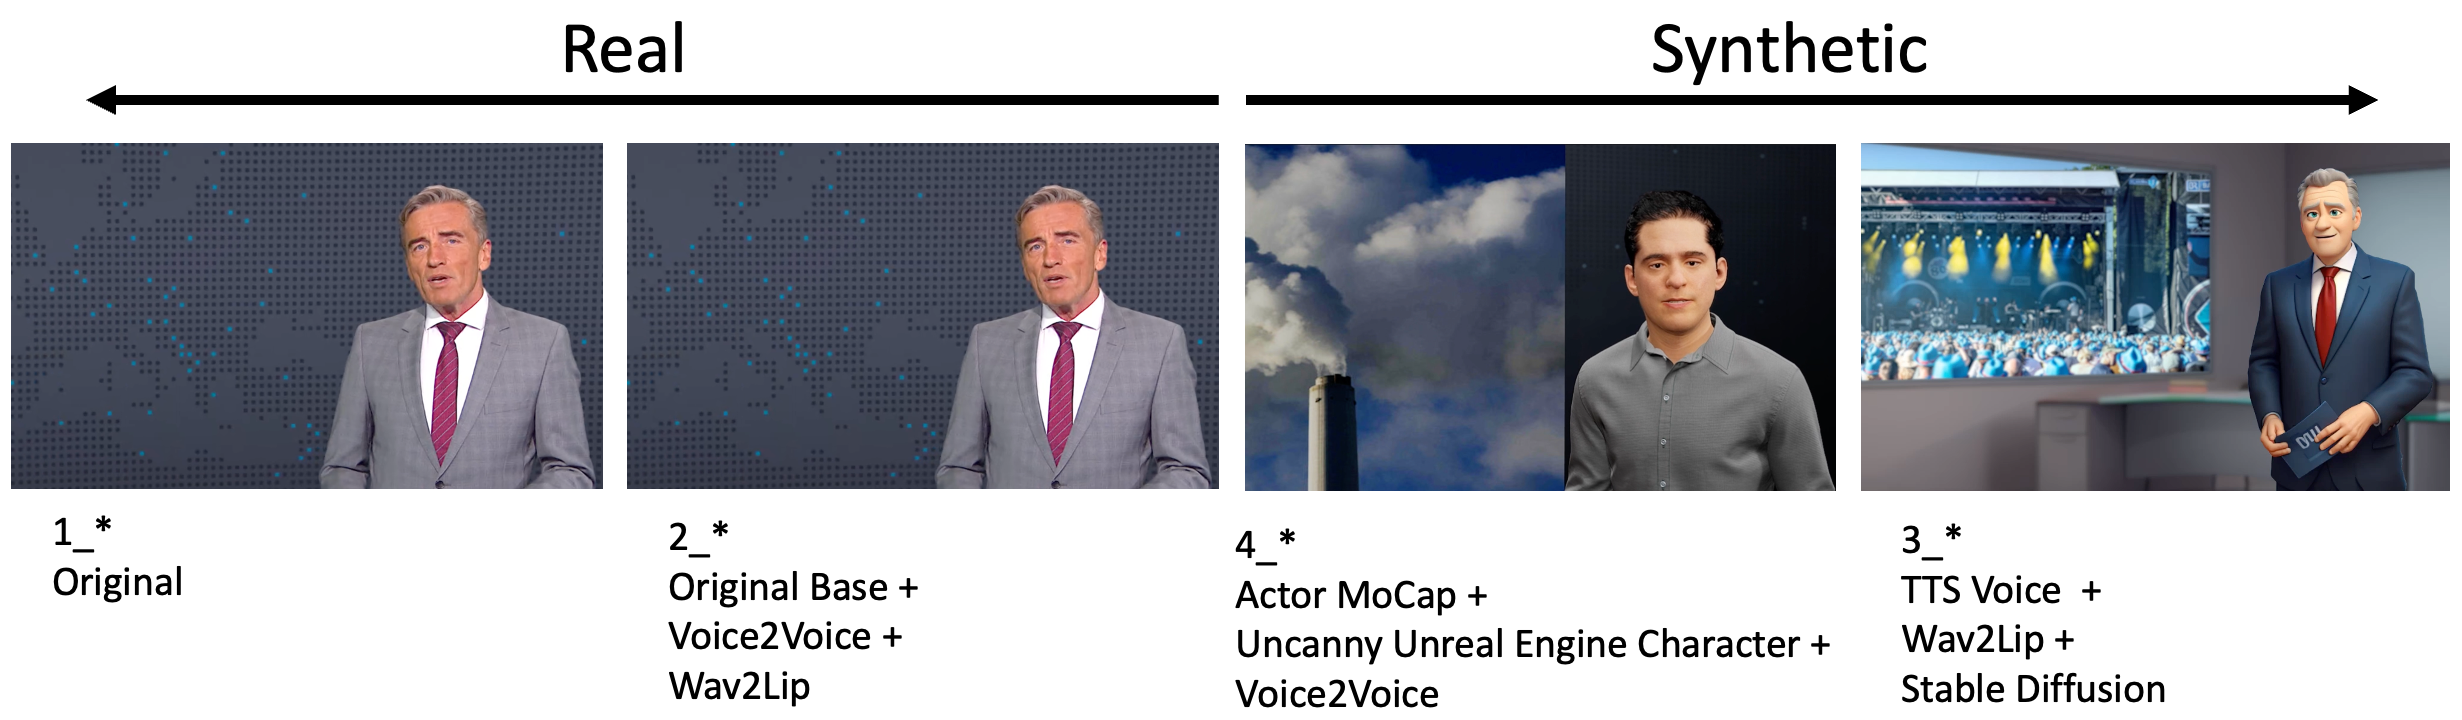
\includegraphics[width=1\textwidth]{./graphics/spectrum-art.png}
  \caption{Spectrum of Artificiality.}
  \label{fig:spectrum}
\end{figure}

On the left end, we have unaltered footage, whereas on the right end, we have a very uncanny-looking and sounding synthetic case. In between these extremes, the amount of artificiality increases from left to right. This spectrum set our goals for what we wanted to create and led to the selection of tools. A more detailed description of the thought process behind the study design is provided in Section \ref{sec:study design}.

Most of the development and training were conducted on a remote Linux server at the University for television and film Munich (HFF) via an \gls{ssh} connection. Many projects featured a Gradio web UI. That way, these tools could easily be accessed from remote hosts via port-forwarding. The \gls{hff} workstation was equipped with an Intel(R) Xeon(R) Gold 6254, 128GB of memory, and a Nvidia RTX A6000 GPU with 48GB of VRAM. The code was checked in at a repository via the Bayerischer Rundfunk (BR). CI/CD was provided with a privately hosted GitLab runner. \\
During the work, two projects were created. The first, Danilo's Voice Toolkit (DVT), provided all necessary implementations for the synthetic voices, including dataset preprocessing and training. The second was the implementation of \gls{w2l} with face upsampling using GFPGAN. Both of the projects were built in a containerized way to ease the installation of dependencies while working on the remote machine without root access. This also ensured high portability across systems in case we had to switch to another machine. Docker images were built with a CI pipeline and then pushed to a private container registry. An instance of \gls{sd} was also used without containerization. For one of the test cases (Actor motion capture in Figure \ref{fig:spectrum}), \gls{ue} was used on a Windows workstation at the \gls{br}. \\
In the following, we provide closer insight into the generation process of several assets, such as \gls{tts}, \gls{rvc}, \gls{sd} and \gls{ue}.

\section{Voice-Cloning Toolkit}
\label{sec:dvt}
While we had some previous experience in the video domain (face swapping and \gls{ue}), we knew almost nothing about the domain of audio fakes. Therefore, we had to figure out feasible ways to create synthetic voices. There are some commercial solutions available that deliver excellent results, but we wanted to see how far we could get with open-source solutions. In the domain of face swapping, there are already integrated toolkits for data gathering, quality control, preprocessing, and training (like \gls{dfl}). This is not the case for voice cloning, which is why we decided to combine several tools into one. These were CoquiTTS, an open-source \gls{tts} engine, and \gls{rvc}, which is used for \gls{v2v} generation (see Sections \ref{sec:tts} and \ref{sec:v2v}). 

\begin{figure}[h]
  \centering
  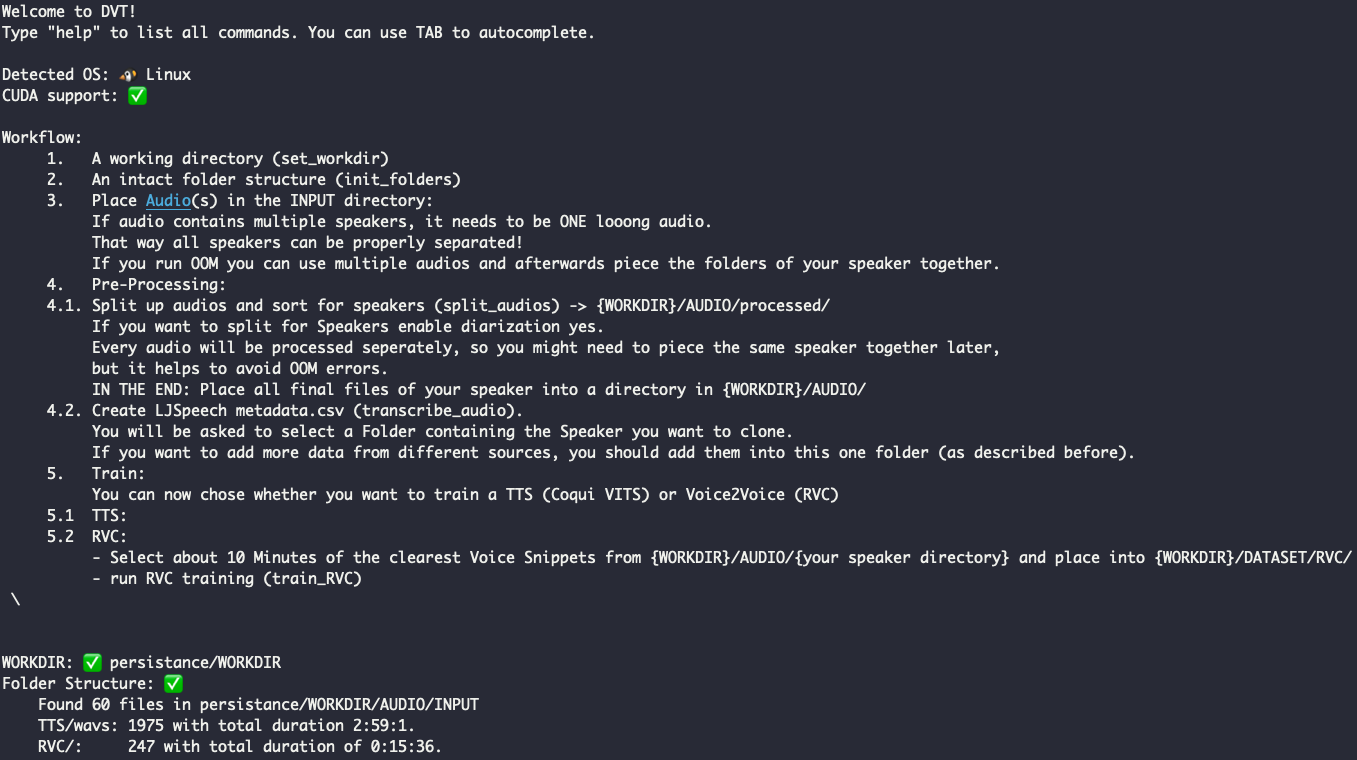
\includegraphics[width=1\textwidth]{./graphics/dvt-screen.png}
  \caption{Start Screen of Danilo's Voice Toolkit (DVT).}
  \label{fig:dvt-interface}
\end{figure}

\gls{dvt} is a command-line interface (Figure \ref{fig:dvt-interface}) that serves as a wrapper for CoquiTTS and \gls{rvc}, and adds methods for importing raw training data and preprocessing it. \\
\gls{dvt} is launched as a Docker container with several forwarded ports. The current directory at launch time is set as the working directory for a certain project. Several folders are created for storing the data, downloading the required models, and persisting them on the local filesystem. After the setup is done, one can start working by placing files in the corresponding \verb|./AUDIO/INPUT/| folder. For the case where \gls{dvt} is running on a remote machine, as it was in most of our cases, we have added a web-based filebrowser to the Docker container, which needs to be started by calling \verb|filebrowser| in \gls{dvt}. Once it is up, one can browse to its port, explore the file system, and upload the required data. This is only reasonable for smaller datasets. In the case of our \gls{tts} training data (30 gigabytes), downloading a tar archive via \verb|wget| and unpacking it was more reliable. 

Next, we treat the preprocessing and training steps of the mentioned technologies (\gls{tts} and \gls{rvc}) in general, then explain the corresponding training data requirements, and in the end, we summarize everything by walking through the whole workflow, from data gathering to training the model. Inference is almost trivial and is well documented for both CoquiTTS and \gls{rvc}.

\subsection{Text-to-Speech}
% General
CoquiTTS is a comprehensive \gls*{tts} tool that can be used as open source, that can be deployed on own systems, and at the same time, drives a commercial variant called Coqui Studio. As explained in Section \ref{sec:tts} there are various ways to convert text to speech. We decided to go with the VITS model. CoquiTTS uses so-called recipes to set up a training run. As they are language specific, we relied heavily on the documentation of \citet{mullerThorstenVoice2023}, who contributed a lot of work to advance the German language within the Coqui project. \\
With the recipes by \Citeauthor{mullerThorstenVoice2023}, it is quite easy to get started. It goes without saying that each training has the option of extensive hyperparameter tuning, but this was far beyond the scope of this paper. We therefore went with the basic settings provided by \Citeauthor{mullerThorstenVoice2023}, except that we increased the batch size to speed up training on our A6000. Most of our development effort did not go into the training but into the dataset preparation, which we will discuss in the next paragraph.

% Preprocessing need
\textbf{Data Requirements} \\
Regarding the dataset structure, it seemed simple: The central resources for training a VITS TTS model are voice samples and corresponding transcription. We discovered from the Coqui community that around two to four hours of speech should deliver the best quality. In order to avoid \gls{oom} errors, the audio needs to be split up into segments with a maximum length of 10 seconds. Lastly, each and every clip needs accompanying text (example in Figure \ref{fig:metadata.csv}). However, getting to the formatted dataset turned out to be quite time consuming with some room for improvement using automation.

\begin{figure}[h]
  \centering
  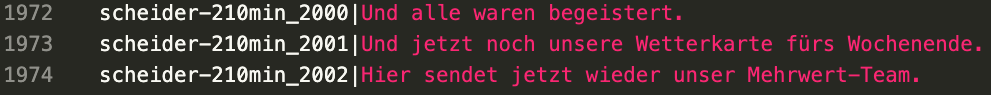
\includegraphics[width=1\textwidth]{./graphics/tts/csv.png}
  \caption{Example of the TTS Training metadata.csv File.}
  \label{fig:metadata.csv}
\end{figure}

% Concrete Workflow
\textbf{Concrete Workflow} \\
A good voice clone starts with a smart target selection. Therefore, we had to determine a suitable environment for our test cases. As we have hinted at earlier, we elaborate on the study design further in Section \ref{chap:study}. TTS voices, in general, perform best with consistent voices where no special (emotional) intonation is required. A newscast is perfect in this regard because of the neutral narration of the content. \\
According to this requirement, we aimed for four hours of speech extracted from the \gls{br} news show \textit{BR24}. We ended up with 60 shows, which accounts for a total runtime of 30 hours. From each, we extracted approximately five minutes of the anchorman's voice. In the end, our dataset contained 2,002 individual clips with transcription. Getting there from 60 hours of news broadcast was quite an undertaking that could never have been feasible without automation, which is where our partially automated preprocessing workflow comes in. We used several tools to aid the dataset creation process, based on various open-source projects \cite{micaAudioSplitterUsing2023}, \cite{harperEndtoEndToolkitVoice2023}: \textit{Pyannote speaker diarization} helps distinguish multiple speakers within one audio track. \textit{OpenAI Whisper} provides audio-to-text transcription. \textit{NVIDIA NeMo} is used for the normalization of the transcribed texts. To give an example of normalization, a transcribed speech of numerals like 42 would be normalized to the corresponding literal "forty-two." This is necessary for the training process to avoid ambiguity, as all input texts are being normalized before being handed over to the \gls{tts} engine. First, we tried a fully automated way of dataset creation, which is depicted in Figure \ref{fig:dvt-tts-original}.

\begin{figure}[h]
  \centering
  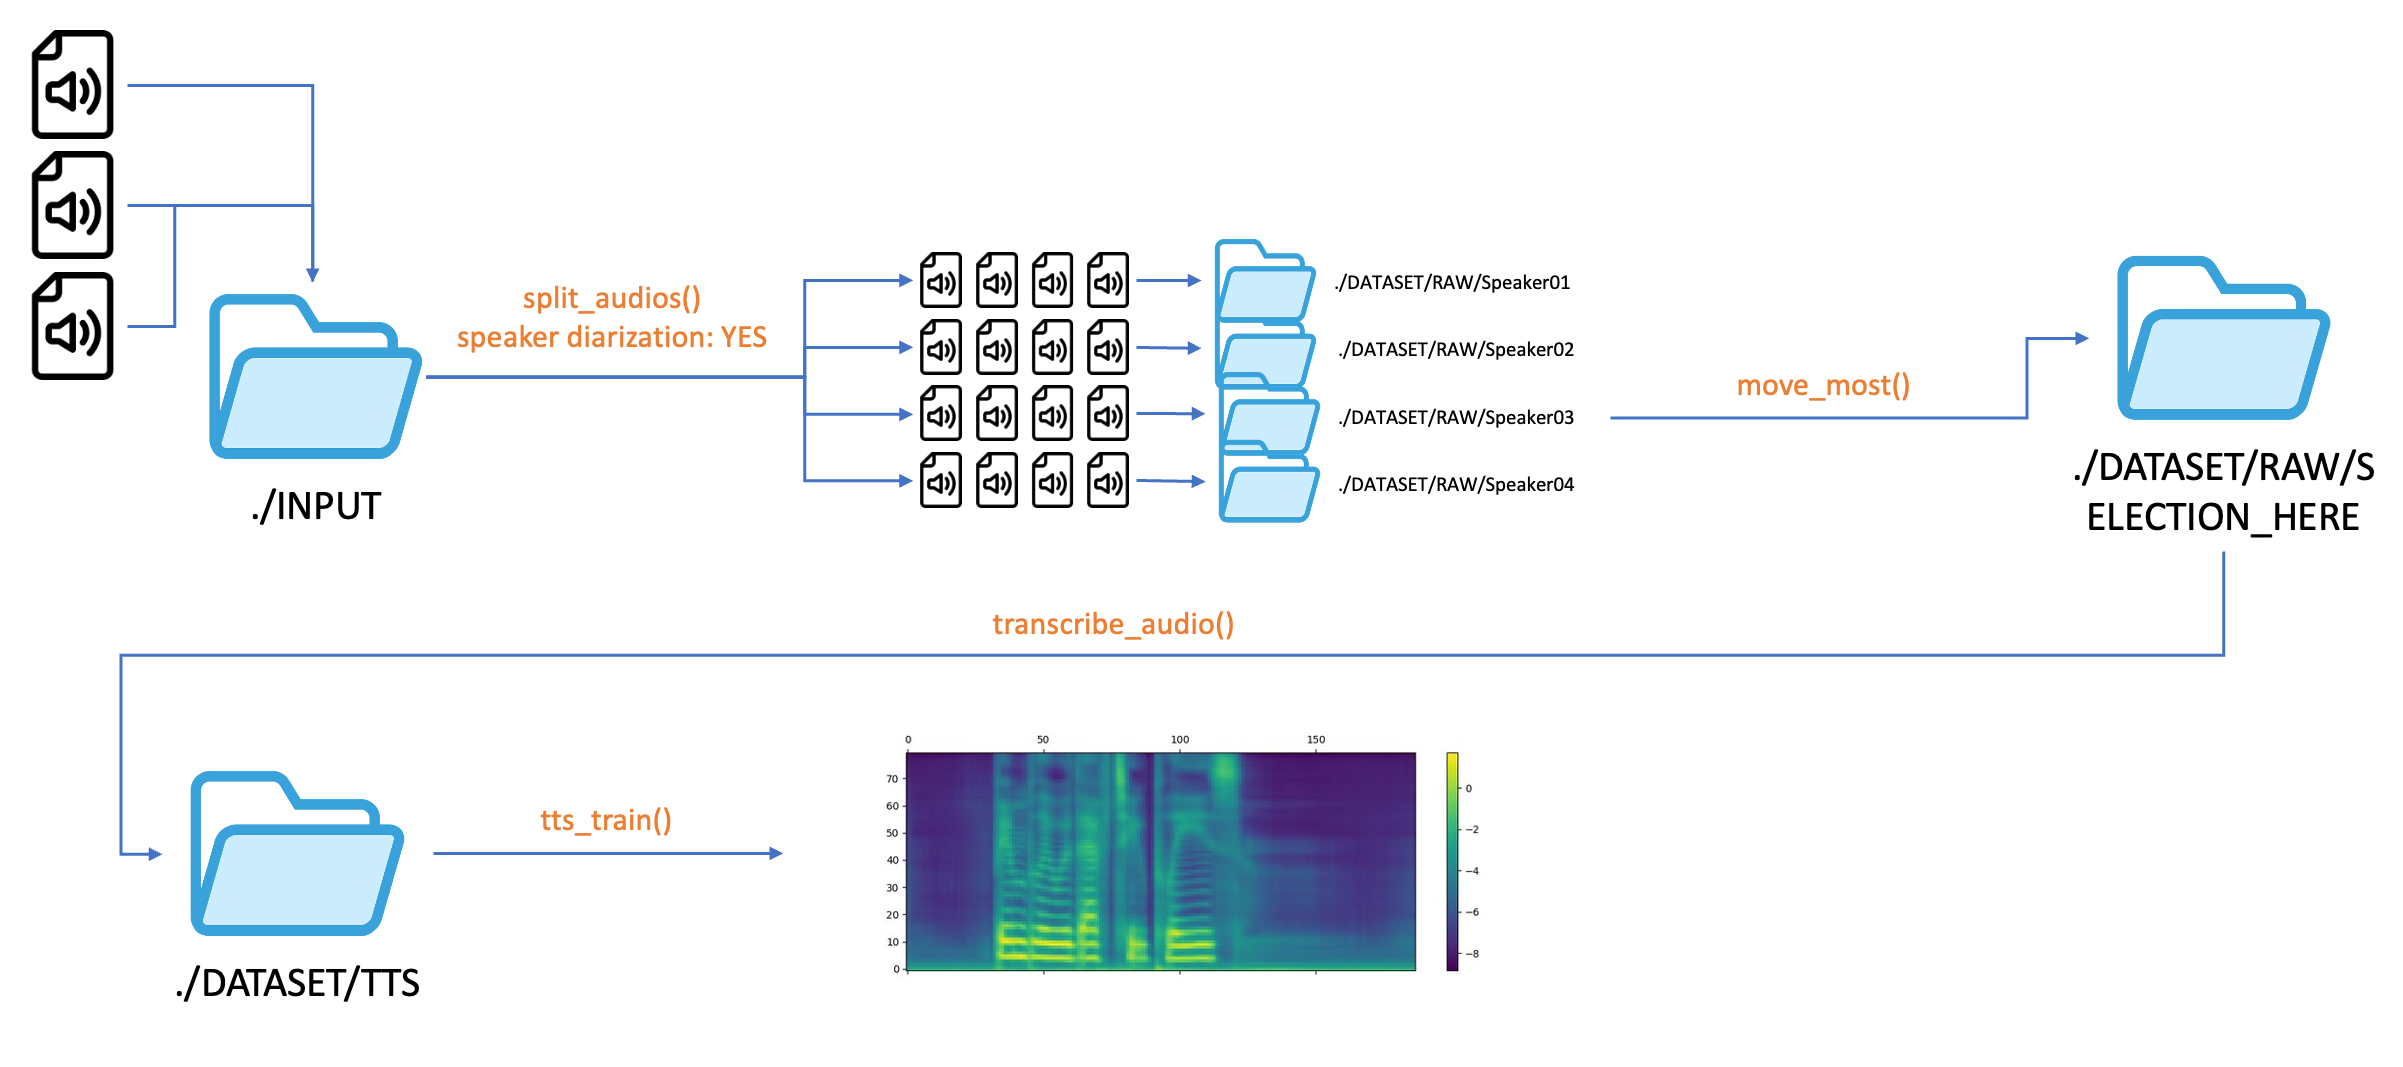
\includegraphics[width=1\textwidth]{./graphics/tts/tts dvt only.png}
  \caption{Fully Automated Data Preprocessing Workflow for TTS in \gls{dvt} (not practicable).}
  \label{fig:dvt-tts-original}
\end{figure}

In this case, we input one or multiple audio files and start the process. Using the tools we just mentioned, the audio is transcribed and marked with a speaker ID.
It is then cut up into pieces of a maximum length of 10 seconds, based on the transcription timecodes, and placed in a dedicated directory based on the speaker ID. The folder with the most files, which is the folder of the anchorman's voice, is moved to the TTS dataset directory, where it is again transcribed and receives the corresponding metadata.csv file with the necessary transcription for \gls{tts} training (see Figure \ref{fig:metadata.csv}).

This process worked quite well, rarely adding false speakers to the anchorman's directory. However, there is one downside to this method, which, unfortunately, makes it unusable. The transcription timecodes provided by Whisper, which are used to cut the audio into pieces, are not accurate enough and often cut parts of a spoken word away. This results in the corresponding TTS voice sounding chopped up as well. This issue could be fixed by using a cutting mechanism that relies on silence in the audio as a cutting signal instead of the transcription timecodes. Although an implementation could have been derived from one of the referenced GitHub projects, we opted against it because we would then lose the speaker differentiation functionality, which is needed because our news segments contained so many different speakers.

\begin{figure}[h]
  \centering
  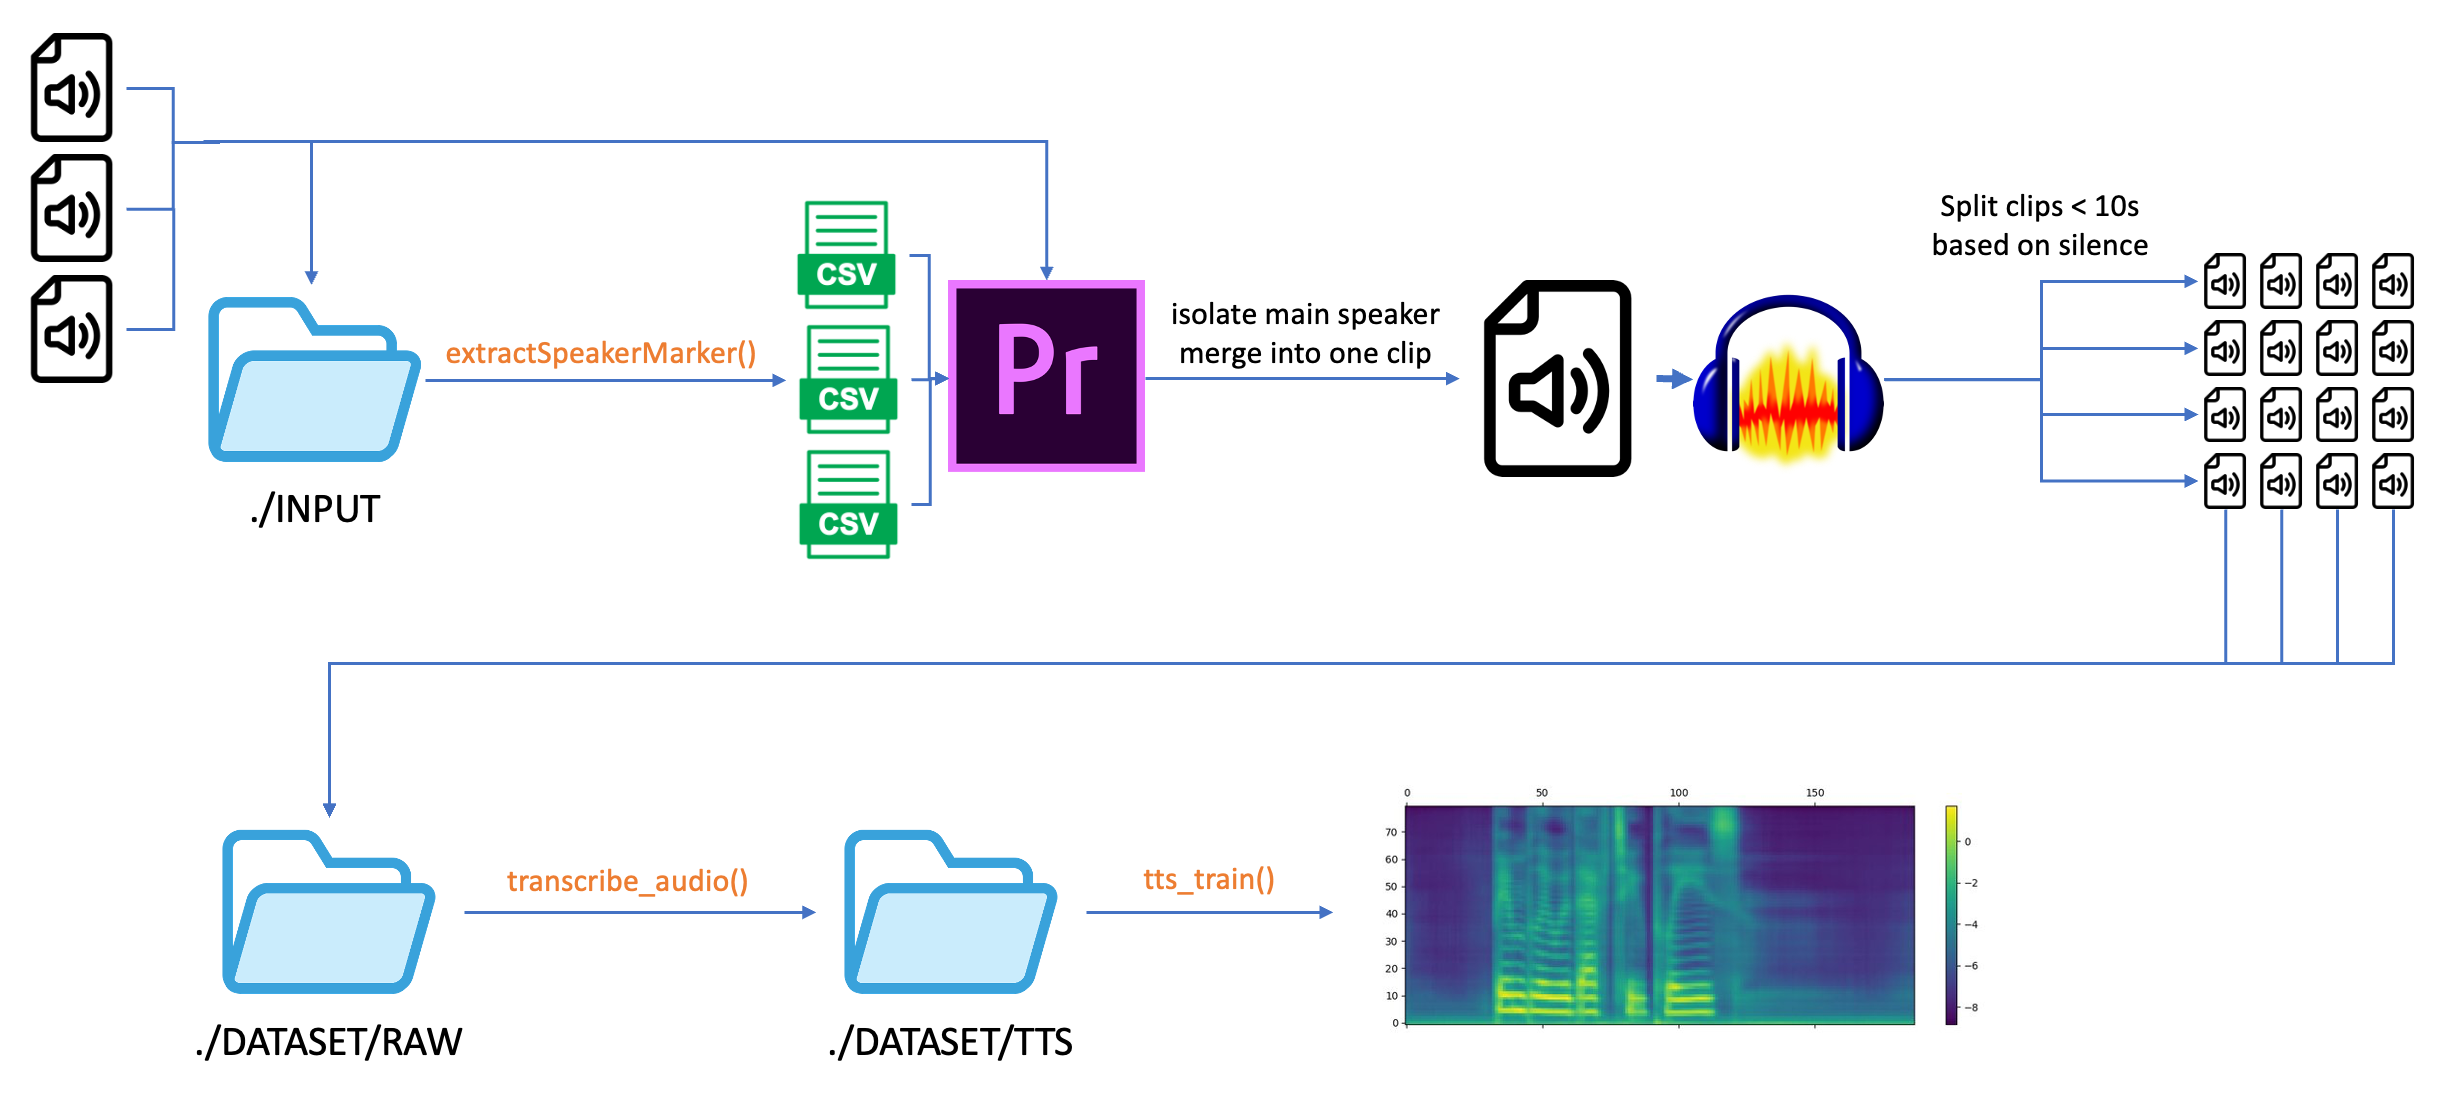
\includegraphics[width=1\textwidth]{./graphics/tts/tts prpro.png}
  \caption{Data Preprocessing Workflow for TTS Training, Using \gls{prpro} and Audacity.}
  \label{fig:dvt-tts-wf}
\end{figure}

Instead, we opted for a more time-consuming, semi-automatic workflow (Figure \ref{fig:dvt-tts-wf}) in conjunction with the previously mentioned tools: Instead of cutting the the audios in \gls{dvt}, we added subtitle export functionality (\verb|extractSpeakerMarker|) for each speaker as a csv file. We then imported the subtitle files of the anchorman into the video-editing software \textit{\gls{prpro}}. Unfortunately, this is not natively supported by \gls{prpro}, which is why we had to rely on an extension called \textit{Markerbox} \cite{montgomeryMARKERBOXFreeMarker}. This turned out to be the quickest alternative to reverse engineering the \gls{prpro} XML format or purchasing software. Finally, we ended up with markings in the timeline (see Figure \ref{fig:premier-markers}). 

\begin{figure}[h]
  \centering
  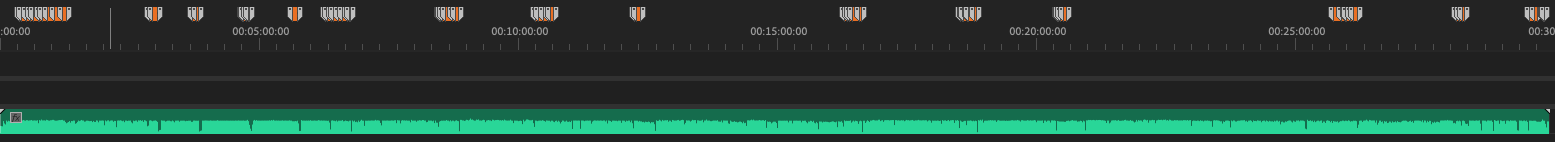
\includegraphics[width=1\textwidth]{./graphics/tts/premier with markers.png}
  \caption{Audio File in \gls{prpro} with Markers of Main Speaker.}
  \label{fig:premier-markers}
\end{figure}

Now, we were able to manually cut away all sections of other speakers very quickly, as we had the visual aid of the markers in the timeline. Once we had isolated the main speaker, we exported the audio clip. From each 30-minute news segment, we extracted approximately five minutes of anchorman-only talk.\\
Next, we needed to chop up the five-minute pieces into audios with a maximum length of 10 seconds based on silence detection. Although this could have been automated, as discussed earlier, we did not want to spend more time on such implementations, as we just wanted to get the dataset ready as quickly as possible. Instead, we chose \textit{Audacity} to confidently detect silence and render out all clips at once. Now that we have all clips cut out cleanly, we uploaded them again into \gls{dvt} to finalize the dataset creation by performing one last transcription with text normalization (\verb|transcribe_audio|) to end up with a correct metadata.csv file (see Figure \ref{fig:metadata.csv}). \\
Once all the files have been generated and placed in the right directories, starting a \gls{tts} training is rather easy. Within \gls{dvt}, we invoke \verb|tts_train| and are guided to start a new training run with a given name and some minor parameters like batch size and training epochs. When the training starts, a TensorBoard is also spun up in the background in order to monitor the training process. It can be accessed with a web browser if \gls{ssh} port forwarding is setup properly (see Figure \ref{fig:tensorboard}).

\begin{figure}[h]
  \centering
  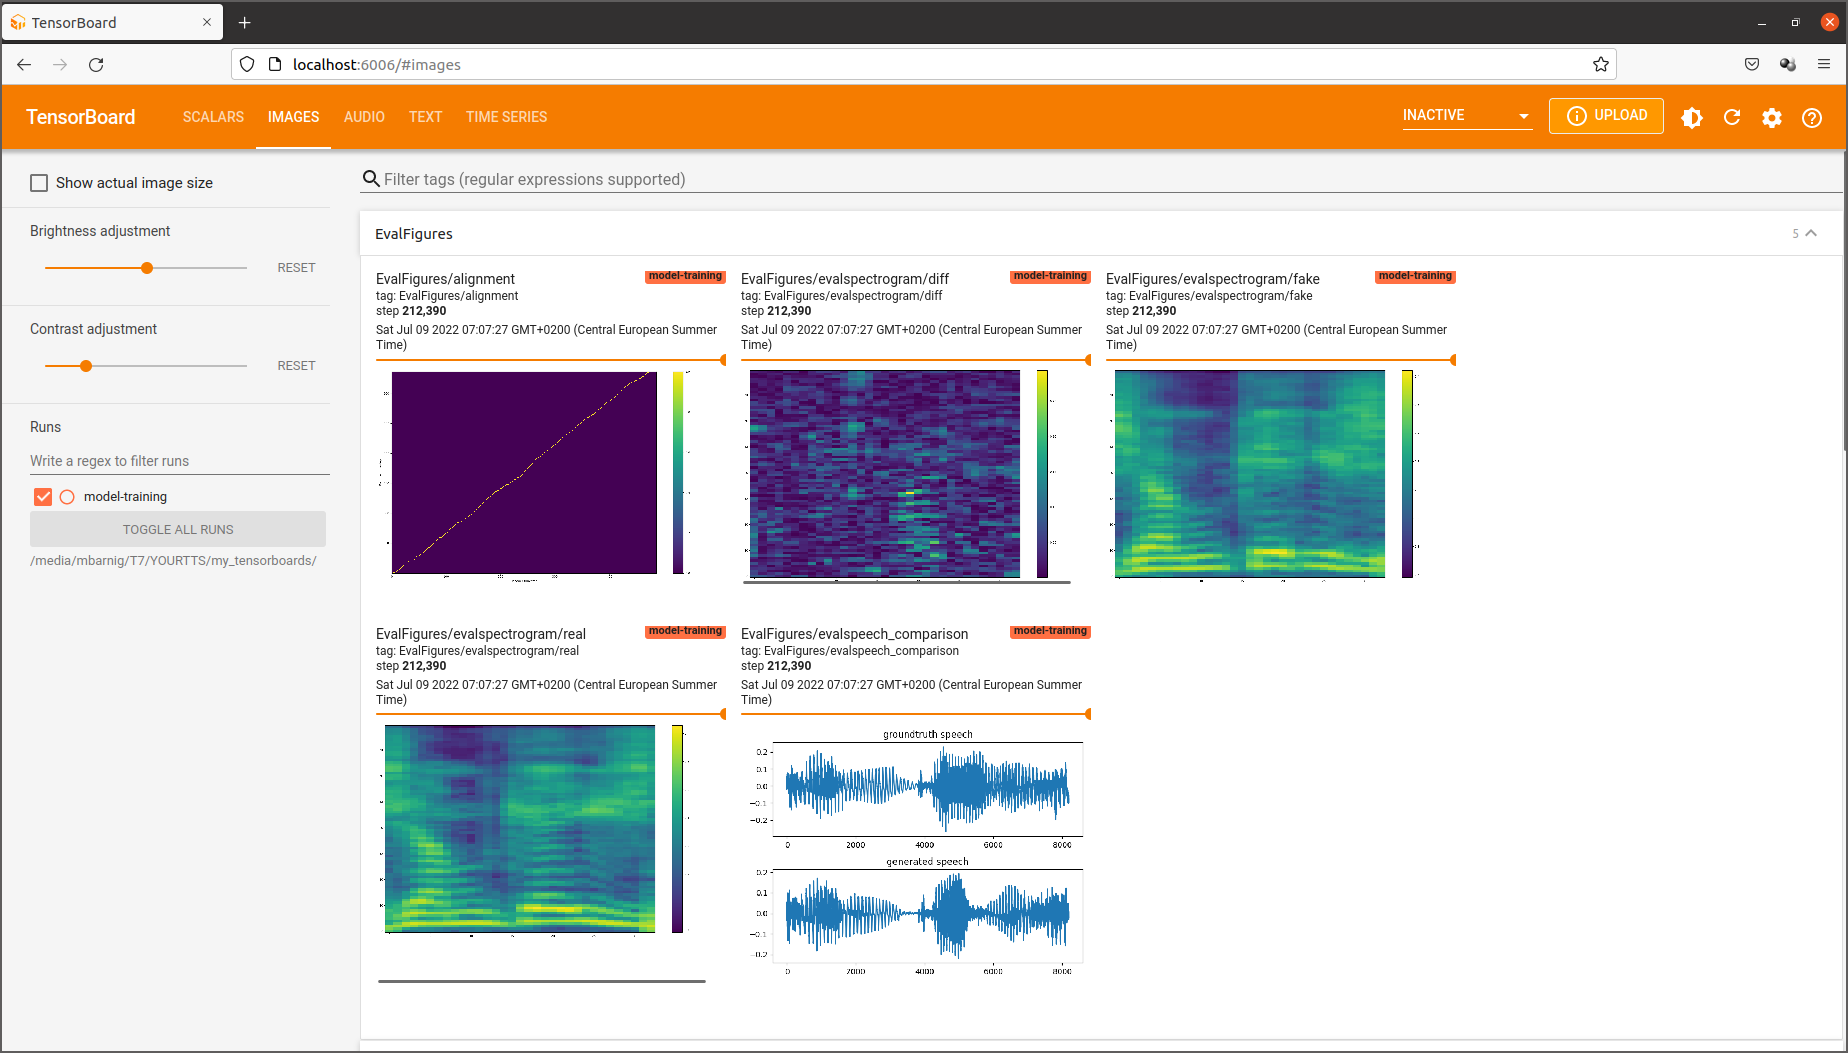
\includegraphics[width=0.8\textwidth]{./graphics/tts/tensorboard.png}
  \caption{CoquiTTS TensorBoard \cite{TensorboardPngMbarnig2022}.}
  \label{fig:tensorboard}
\end{figure}

TensorBoard provides many interesting insights into the training process, including plotting loss graphs, showing mel spectrograms, and preparing generated audio files for easy playback. By judging these different sources, one can determine, whether the training is finished. 

% Inference
\textbf{Inference} \\
Now that the model is trained, inference is straight-forward. For further details, we encourage checking out the CoquiTTS documentation. A basic CLI command to synthesize a sample looks like this:
\begin{lstlisting}
  tts --model_path "path/to/checkpoint.pth" --config_path "path/to/config.json" --out_path "path/to/outputFile.wav" --text "Text to be synthesized."
\end{lstlisting}

\textbf{Possibilities for Quality Improvements} \\
After the \gls{tts} audio is generated, it might be necessary to do some manual corrections to the audio track. Most imperfections are related to odd sentence flow or chopped consonants towards the end of a sentence. This can be done with any editing software. We rarely had to correct anything for our model, but we certainly tried to edit the audio to the right positions of the video so that it matched the scene as well as possible. In addition, we could also upscale the quality by applying \gls{rvc} on top of the \gls{tts}-generated audio. While \gls{rvc} could not correct odd sentence flow or chopped words, it could add some depth to the speech quality. We decided against this improvement to have more distinctiveness between the test cases, but in a production system, this might be a viable solution to improve \gls{tts} quality in the future. 

\subsection{Voice-to-Voice Conversion}
%General
To convert our speech recordings to the voice of the anchorman, we used \gls{rvc}. Compared to \gls{tts}, \gls{rvc} is straightforward. Regarding \gls*{dvt}, almost no adaptations to the original \gls*{rvc} \cite*{RVCProjectRetrievalbasedVoiceConversionWebUI2023} code were made. \gls*{dvt} mostly serves as a CUDA runtime environment to provide all drivers, dependencies, and AI models required to run \gls{rvc}. We added the aforementioned \verb|filebrowser| to make file transfers to a remote GPU server easier. Of course, we can employ our preprocessing tools to aid the dataset generation process. As depicted in Figure \ref{fig:rvc-gradio}, \gls{rvc} features a Gradio user interface with several tabs at the top, most importantly, training and model inference. For training, most hyperparameters are already set; only the dataset location needs to be set. Inference is also done within the GUI. \\
\gls{rvc} was initially based on a project for singing voice conversion, a feature that is implemented in \gls{rvc} as well. During inference, voices, as well as singing voices, can be converted to previously trained models. Before converting a singing voice, a clean vocal track is needed. For that reason, the developers added the \gls{uvr} to a separate tab of the GUI. With this utility, the main vocals can be separated from background music to convert the voice properly without background noise.

%Data requirements
\textbf{Data Requirements} \\
For a good \gls{rvc} model, only 10 minutes of speech are required. It is also less important than for \gls{tts} that sentences are complete. When a word was cut off, we did not experience any issues. Therefore, we could fully use the speaker diarization and cutting process we initially built for \gls{tts}. 

%concrete Workflow
\textbf{Concrete Workflow} \\
As can be seen in Figure \ref{fig:rvc-wf}, the preprocessing workflow is much leaner compared to \gls{tts}.
\begin{figure}[h]

  \centering
  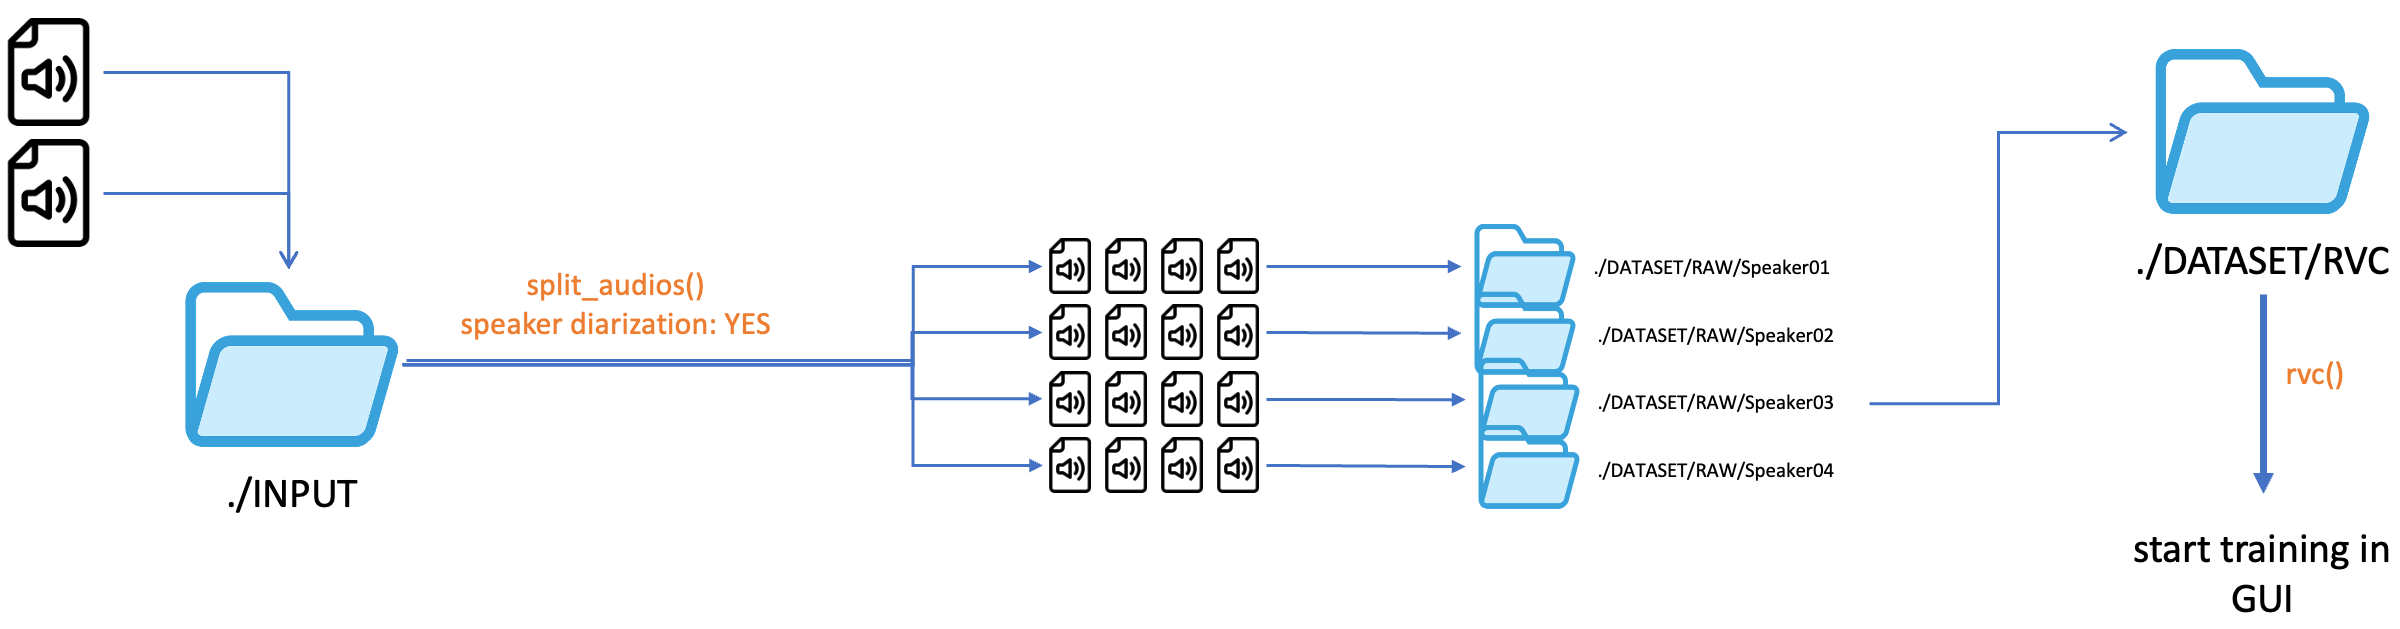
\includegraphics[width=1\textwidth]{./graphics/rvc/rvc-workflow.png}
  \caption{Data Preprocessing Workflow for RVC Training.}
  \label{fig:rvc-wf}
\end{figure}

We know that we can extract approximately five minutes from every 30 minutes of news shows, and we need two of them for the 10 minutes of training material. These are placed in the INPUT directory. Invoking DVT's \verb|split_audios| method triggers the speaker-diarization and segment-splitting workflow based on a transcription and corresponding timecodes. \\
We end up with a subdirectory for each speaker of each input audio. We can now use \verb|filebrowser| to listen through the speakers and then move the right audio into the \verb|DATASET/RVC/| directory, or we can use \verb|move_most|, which will go through all speaker folders and move those with the most data into \verb|/DATASET/RAW/SELECTION_HERE|. Now, we can move all data from here into \verb|DATASET/RVC/|. \\
Once 10 minutes of snippets, all under 10 seconds, are in the \verb|DATASET/RVC/| directory, we can start the \gls{rvc} UI within \gls{dvt} using \verb|rvc|. From there, we can start the training by entering the dataset directory and clicking two buttons. The GUI, together with the online documentation, is quite easy to follow and thus is not explained further. This also applies to inferencing or converting voices with \gls{rvc}.

\section{Lip Remapping}
 After we created the auditory part, we needed to adjust the visual part as well. This was done, in all cases except the \gls{ue} case, with the help of \gls{w2l} \cite{mukhopadhyayWav2LipAccuratelyLipsyncing2023}. Like the development of \gls{dvt}, we implemented the \gls{w2l} project as a portable Docker container as well. Different from \gls{dvt}, the \gls{w2l} container features a Gradio interface only (see Figure \ref{fig:w2l-gradio}). This eases the file-handling process as the host file system is not required. Everything is stored inside the container during runtime and can be downloaded via the UI in the web browser.
 \begin{figure}[h]

  \centering
  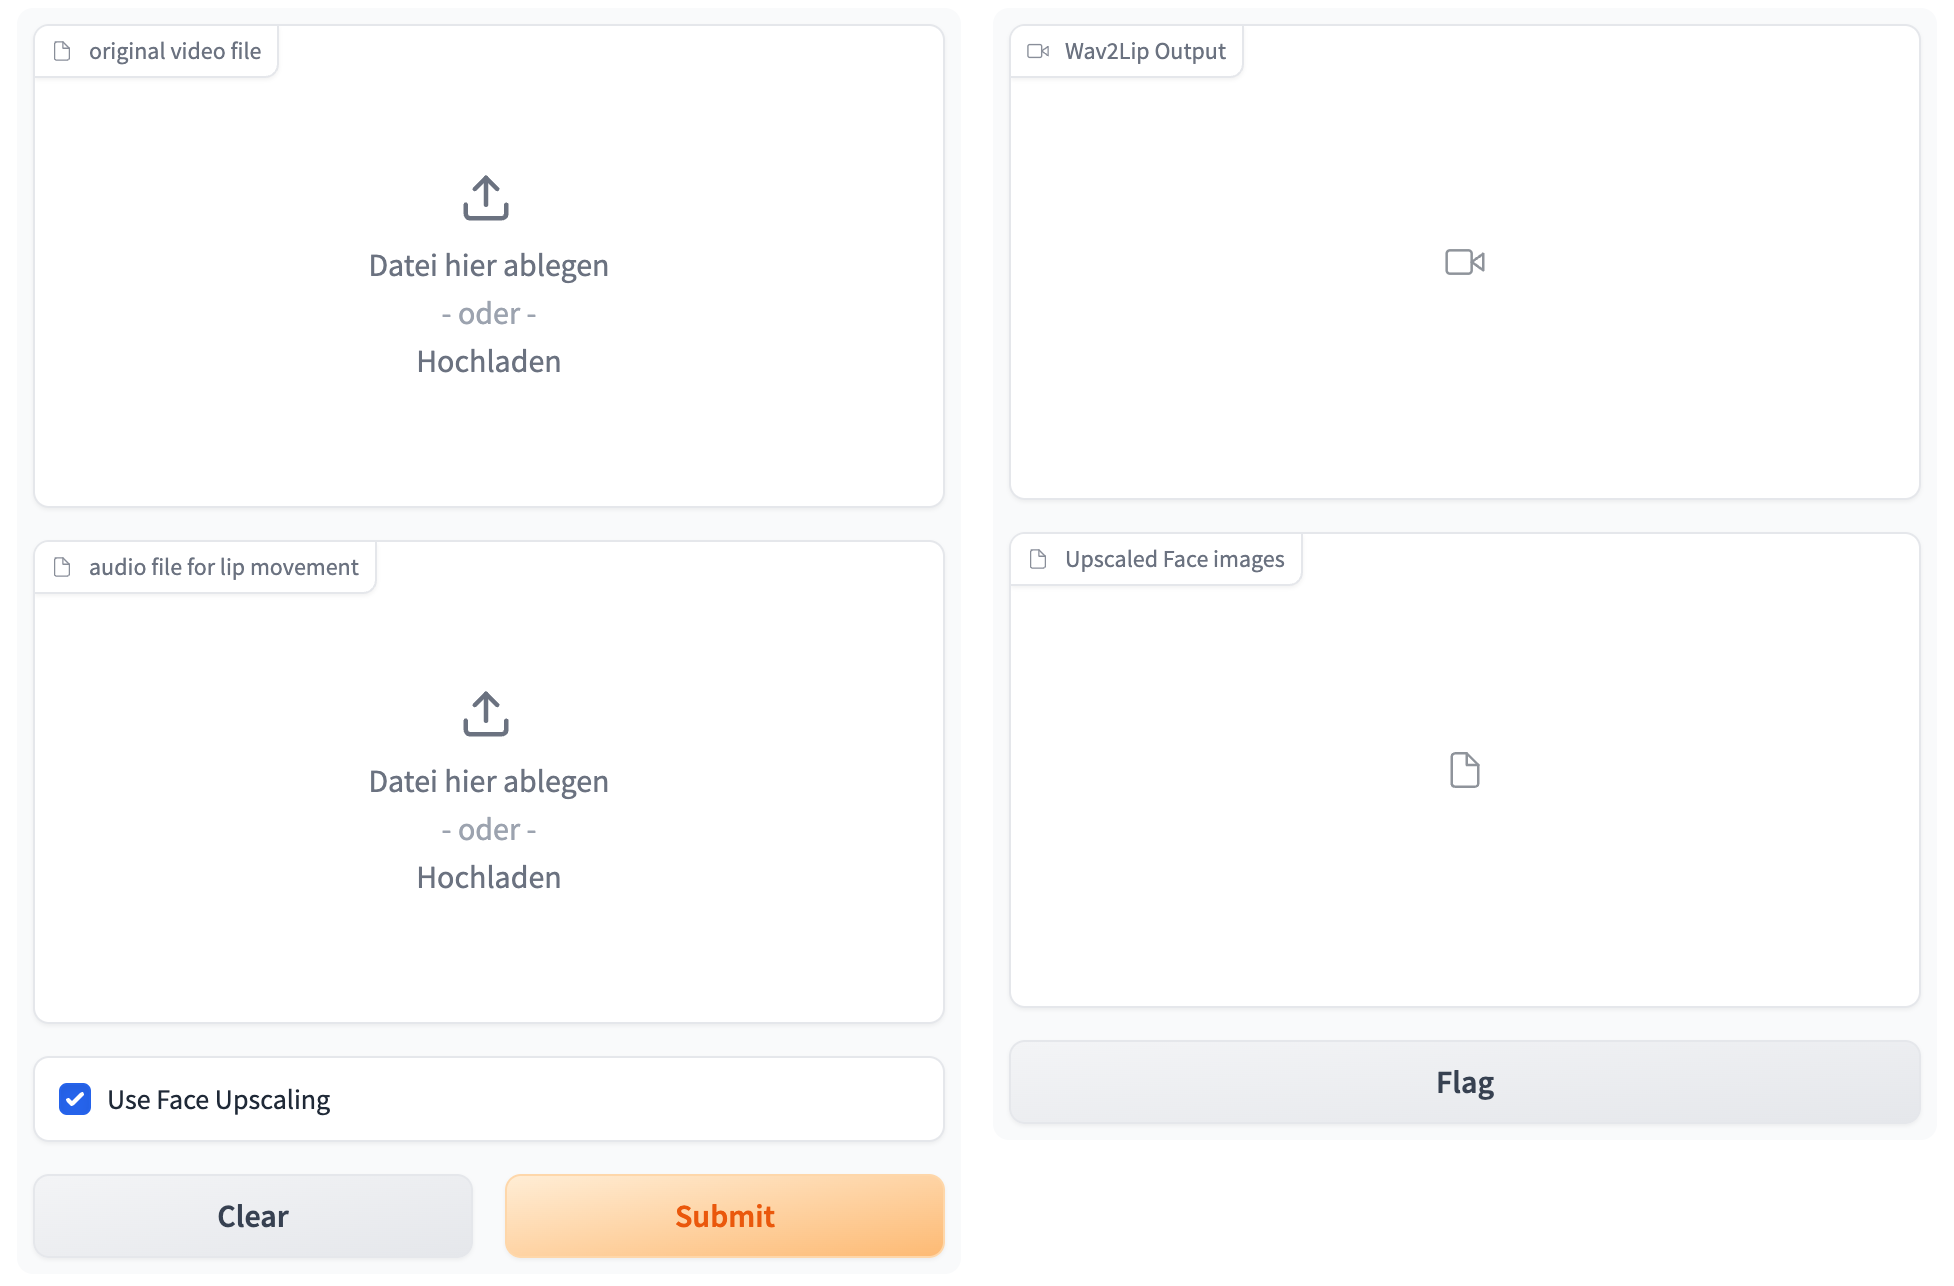
\includegraphics[width=0.9\textwidth]{./graphics/wav2lip/w2l-gradio.png}
  \caption{\gls{w2l} Gradio Webinterface.}
  \label{fig:w2l-gradio}
\end{figure}

\textbf{Concrete Workflow} \\
The usage is fairly simple: uploading a video and corresponding audio to the interface and executing \gls{w2l}. To create the best results regarding timing, it is advised to precisely edit the audio and video beforehand so that they have exactly the same length. \\
As mentioned earlier, one downside of the public implementation of \gls{w2l} is that its lip-synching model has been trained at a very low resolution of 96 x 96 pixels, which is not sufficient for today's standards of high definition. At a resolution of 1080p, a resolution of at least 256 x 256 is required. To mitigate this problem, we added a facial reconstruction library in the form of \textit{GFPGAN}, inspired by the Wav2Lip-GFPGAN GitHub project \cite{sainyAjaysainyWav2LipGFPGAN2023}.
The complete workflow is depicted in Figure \ref{fig:w2l workflow} below.

\begin{figure}[h]
  \centering
  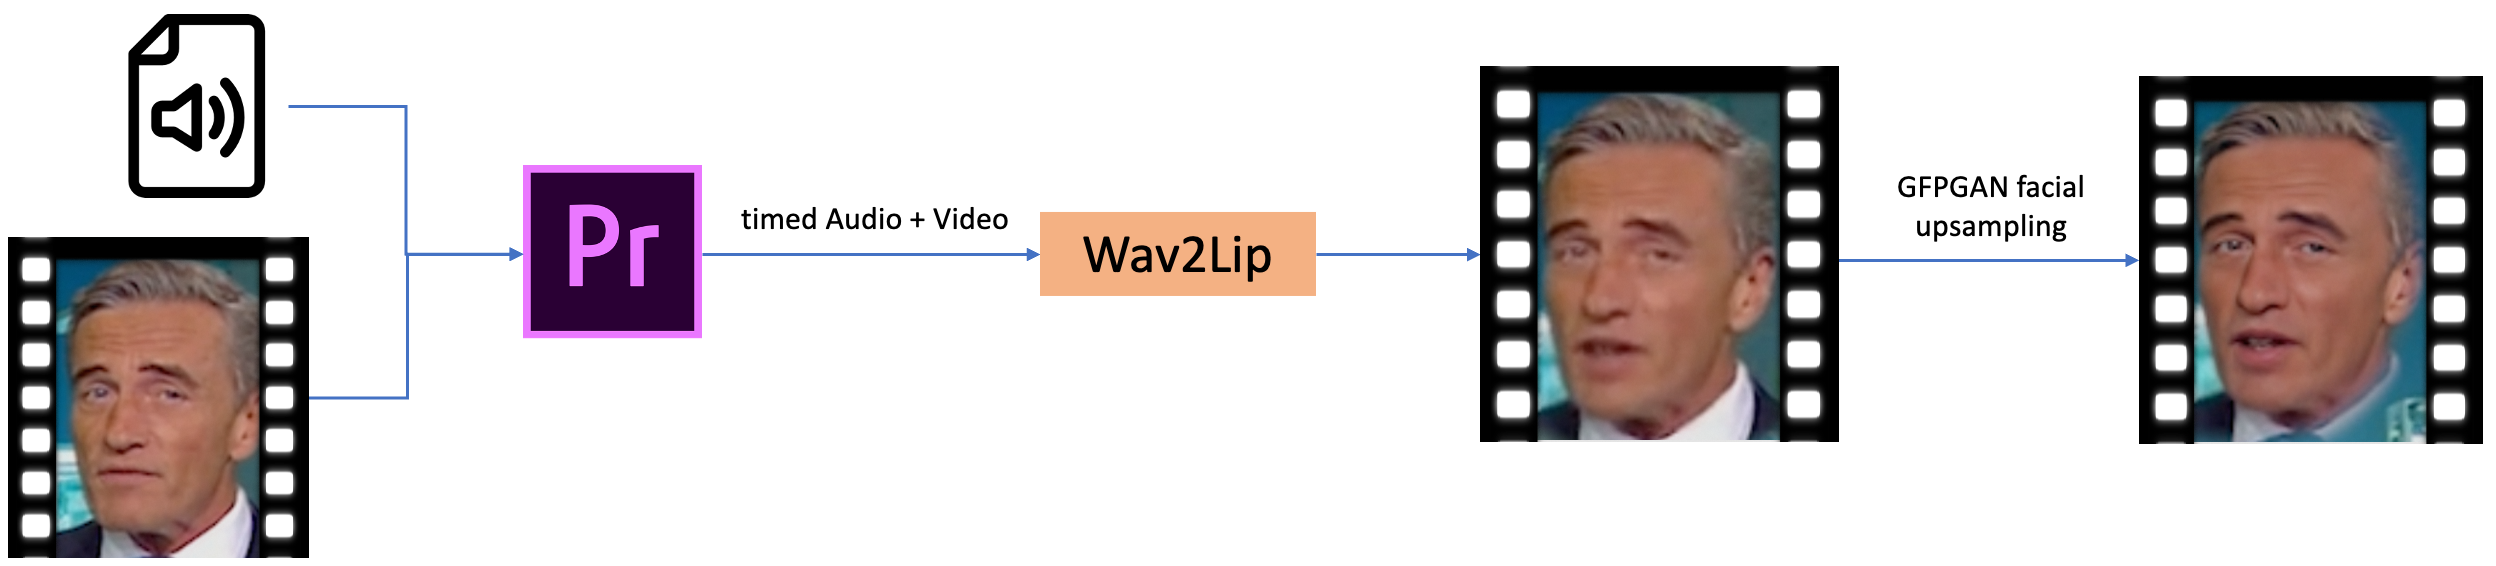
\includegraphics[width=1\textwidth]{./graphics/wav2lip/w2l workflow.png}
  \caption{Workflow for Wav2lip.}
  \label{fig:w2l workflow}
\end{figure}

Since the GFPGAN upsampling significantly increases the processing time, it can be disabled for quicker testing. Once finished, the video can be downloaded as an image sequence to a local computer. The reason we chose to work with the image sequence instead of an already merged video is that we wanted to reduce the video conversion touchpoints, as we lose quality with every lossy video encoding. Lastly, the image sequences and audios need to be put back together in \gls{prpro}. In some instances, minor retouches were performed in \gls{ae}.

\textbf{Possibilities for Quality Improvements} \\
The process of GFPGAN upsampling every frame individually introduces a small flickering effect in the facial area of the final rendering. This could be mitigated further with deflickering software, but this is one step we chose not to carry out. As an alternative to GFPGAN, it would have been possible to use the previously discussed face-swapping technologies (Section \ref{sec:face-swapping}) to upsample the \gls{w2l} results. We tested the workflow using \textit{Inswapper}, and the results were not satisfying: (1) When using Inswapper on top of the blurry \gls{w2l} output, the result was blurry as well. It seems that Inswapper applies the blurriness to the generated image as well. This makes total sense in the case of motion blur, but it is counterproductive in our case. (2) Using Inswapper on top of GFPGAN-upscaled results did not work either. Still, a little bit of flickering could be perceived, probably because Inswapper tries to mimic the lighting as well as possible. \\
Probably the best solution would have been to use \gls{dfl}. There are some examples on the Internet confirming \gls{w2l} in combination with \gls{dfl} as a working approach. We decided against the use of \gls*{dfl} because of the added effort of training a \gls{dfl} model (two weeks) and the significant postprocessing needed for every single one of our videos. 


\section{Stable Diffusion Video}
\label{sec:sd-video}
To further increase the degree of artificiality in our videos, we decided to alienate the images using \gls{sd}. In Section \ref{sec:stable-diffusion-bg}, we have established image generators as a versatile tool for many applications. Its astonishing development can be credited to the active community to a large degree. For our project, we used the \gls{auto1} \gls{sd} front end with several extensions for better video processing. \\
There are two challenges with \gls{t2i}: \textit{control} and \textit{consistency}. A prompt to resemble a news anchor inside a TV studio will never remotely resemble the real anchorman. As a first step, the random seed needs to be fixed. To increase the consistency at least a bit, every frame needs the same random noise as a starting value. However, this cannot help us with the movement of an object within the scene. In our case, it is especially important that at least the lips somewhat match the spoken audio. Luckily, the \gls{sd} community had come up with a solution: ControlNet.

\begin{figure}[h]
  \centering
  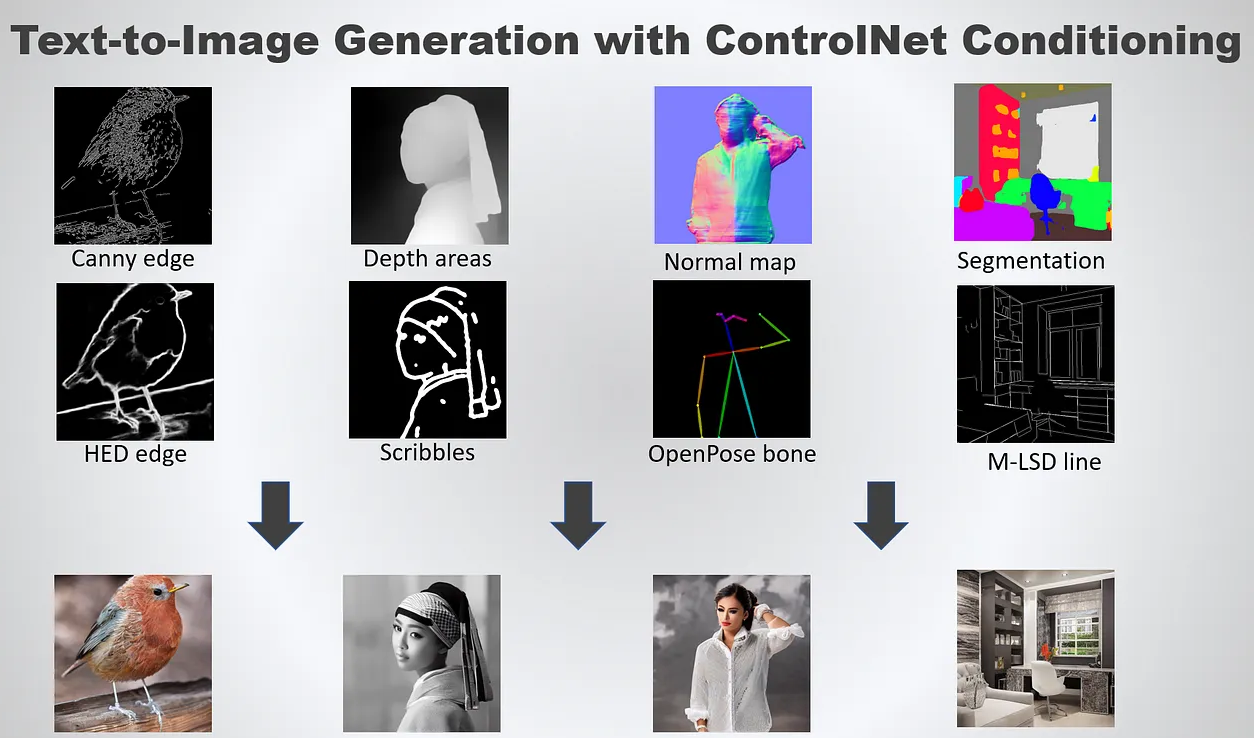
\includegraphics[width=0.8\textwidth]{./graphics/diffusion/ControlNet.png}
  \caption{ControlNet Examples \cite{foongIntroductionControlNetStable2023}.}
  \label{fig:ControlNet}
\end{figure}

In addition to text prompts, ControlNet enables the user to input additional features (see Figure \ref{fig:ControlNet}) such as scribbles, various edge detection outputs, depth maps, normal maps, segmentation maps, and many more. The most important controller for our purposes, however, was \textit{OpenPose}, which is how we created results as shown in Figure \ref{fig:scheider-real-sd}. OpenPose extracts the gestures and facial expressions from the anchorman and feeds them into the diffusion process. For gestures and even finger movements, OpenPose works quite well. Regarding facial movement, OpenPose does not provide enough markers to track faces with high fidelity. Although many facial expression details are lost in the process, it is enough to somewhat animate the mouth and eye movements.
Now, after we mitigated the \textit{control} problem, we face the next issue. For a moving image impression, we need multiple frames per second: for digital video, 25 \gls{fps}, to be precise. Even if ControlNet helps a great deal regarding the controlled categories (gesture and facial expressions), the rest of the image looks a little different in each frame. This introduces some flickering during playback. Figure \ref{fig:controlnet-issues} shows some of these effects.

\begin{figure}[h]
  \centering
  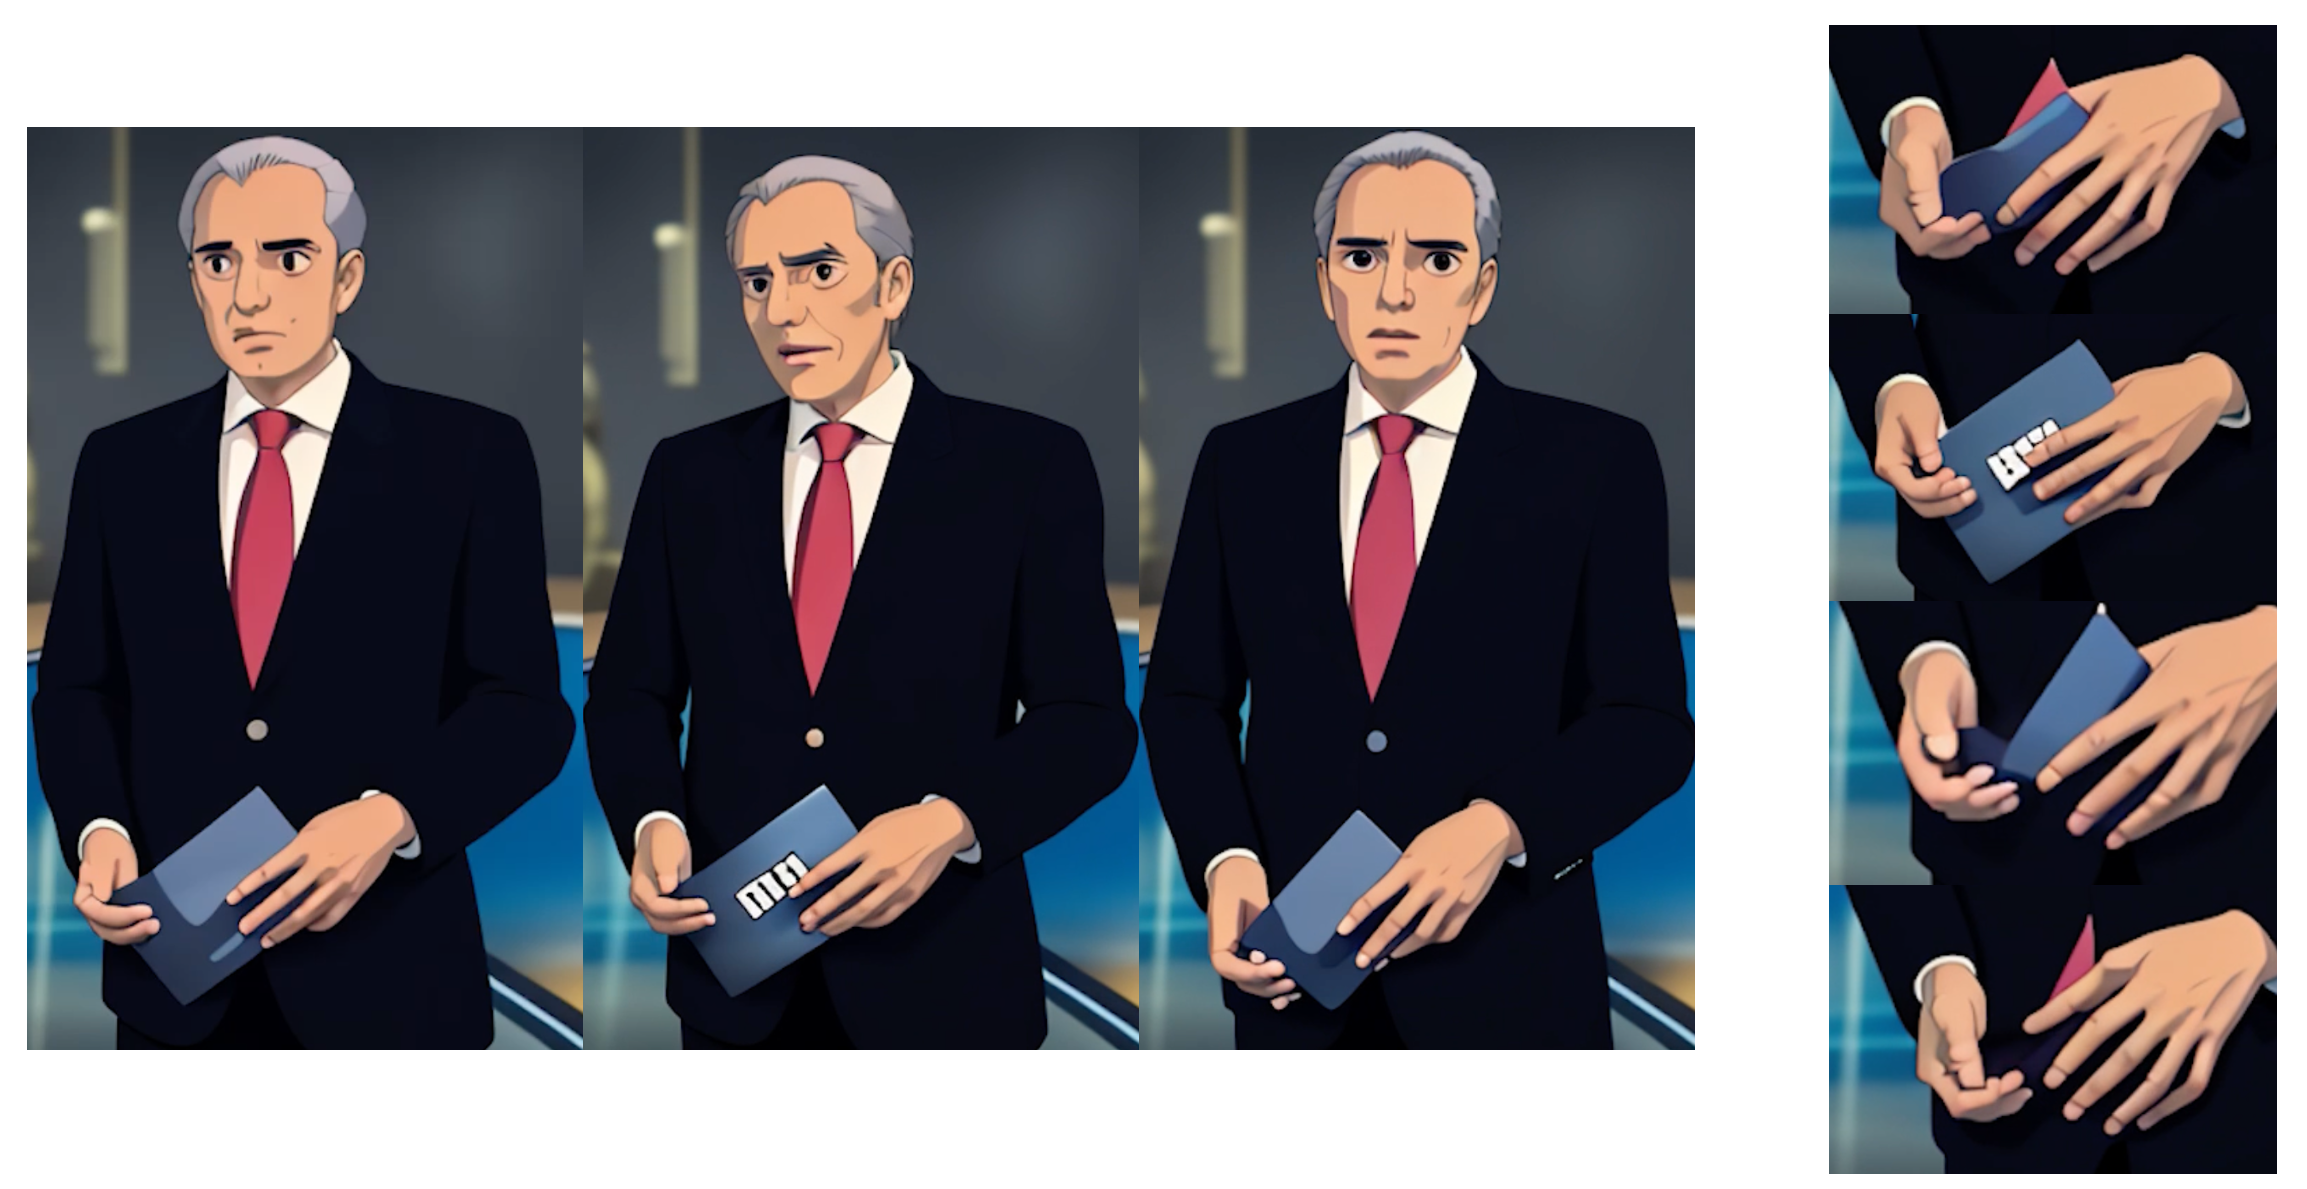
\includegraphics[width=0.8\textwidth]{./graphics/diffusion/ControlNet-issues.png}
  \caption{Consistency Problems: Studio Ghibli LoRa, Fixed seed, ControlNet OpenPose.}
  \label{fig:controlnet-issues}
\end{figure}

While the posture of the hands is often okay, the card the actor is holding slightly changes in each frame. These effects appear everywhere in the image, for instance, in the color of his buttons and his tie. Watching these inconsistencies at 25 \gls{fps} is very unpleasant and greatly reduces the overall quality of the video. One way of fixing consistency is by using other ControlNet layers like depth maps or \textit{Canny}. A downside of increased ControlNet activity is reduced control using the text prompts. Consistency is also model-dependent, so we tried out various models. After much trial and error, we ended up with the results seen in Figure \ref{fig:scheider-real-sd}.

\textbf{Concrete Workflow} \\
Prior to the \gls{sd} input, the base videos were created using Wav2Lip and \gls{tts} or \gls{rvc} as described earlier. We cropped the video to feature only the actor. This reduced processing time, increased quality, and improved consistency because the area of attention was smaller and more focused. \\
After generating the main actor, we composited him into the final clip using \gls{ae}. Because the background was  twitching as well due to consistency issues, we decided to key it away, as only the actor is important for the scene. We accomplished this by generating a depth map with \gls{auto1} and using the map as the isolation criterion. Afterwards, we composited the actor on a studio image background. The full \gls{sd} workflow is depicted in Figure \ref{fig:sd-full-workflow}.

\begin{figure}[h]
  \centering
  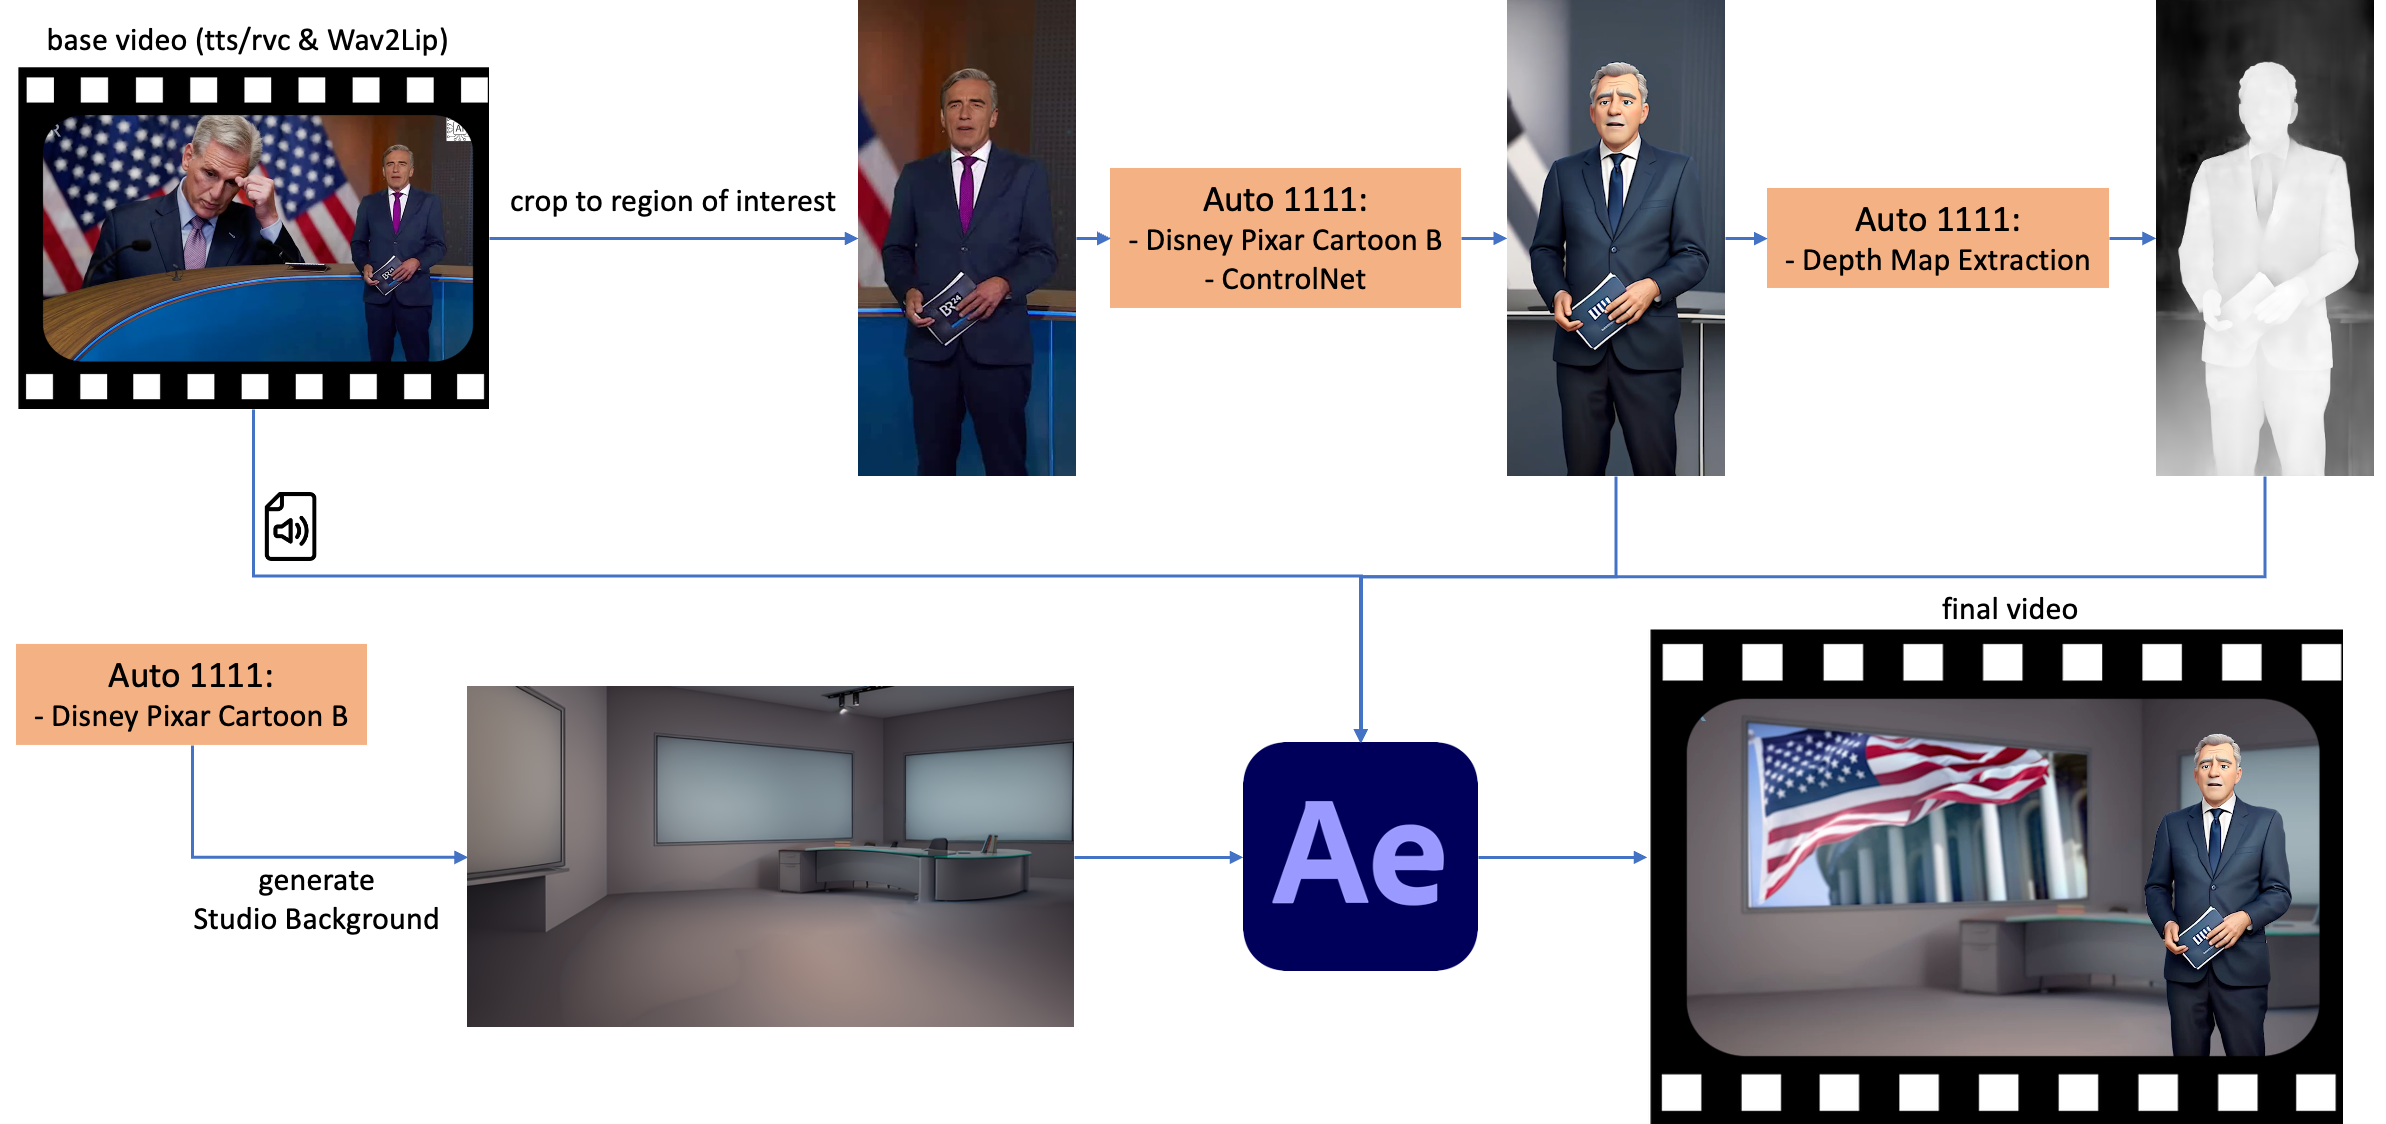
\includegraphics[width=0.9\textwidth]{./graphics/diffusion/sd-workflow.png}
  \caption{Our Stable Diffusion Video Workflow.}
  \label{fig:sd-full-workflow}
\end{figure}

At the time of writing, we can report that the ControlNet workflow might already be outdated. In July 2023, \textit{Animate Diff} was released, which offers an alternative workflow to ControlNet. During the creation of our experiments, Animate Diff was not tested and documented well enough, so we could not test it in a reasonable timeframe, but it seems in some cases to deliver much better results than ControlNet in both dimensions of control and consistency. In November 2023, Stability AI released the first \gls{svd} foundation model, which shows much future potential. In January 2024, Google released Lumiere, their video generation tool, which is just another example of the fast pace of current innovations.

\section{Game-Engine: Unreal Engine}
As another asset in our artificiality spectrum (4\_* in Figure \ref{fig:spectrum}) we decided to repurpose an existing project conducted in \gls{ue}. It was part of a master's practical at \gls{lmu} during the summer semester of 2023, under the supervision of Prof. Dr. Johanna Pirker. A detailed report of the practical is available as well, but we include the most important findings in the following section. The goal of the practical was to glimpse into the possibilities of virtual production, learning basic 3D modeling and the operation of \gls{ue} and accompanying software. To give the goal a concrete example, we wanted to recreate a news show from \textit{\gls{br}} Television, which made it an ideal candidate for this paper as well. \\
Although it is quite easy to get started with \gls{ue}, realizing complex projects is a difficult undertaking. The main reason lies in the fact that \gls{ue}'s main purpose is to aggregate many different assets and give them logic. Surely it is possible to model, rig, and animate characters within \gls{ue}, but there are various specialized tools for all of the named tasks: Maya, Zbrush, Blender, and iClone Character Creator, to name a few. Doing all these things is certainly possible in \gls{ue}, but it has its limits. Mastering several tools takes a lot of time, which is why we focused only on the integrated tools of UE. It is quite impressive what can be done with only \gls{ue} in approximately 200 hours of work, but it is also clear that there is much room for improvement. \\
The generated results have neither to do with \gls{genai} nor do they look particularly impressive, probably because the character is quite uncanny. Still, we decided to employ the technology for our paper, and virtual production is expected to play a huge role in the coming year regarding synthetic media. Because of its relevance to synthetic media, we decided to include thorough documentation of the unreal workflow. \\
We expected the uncanny avatar to produce the worst credibility due to the uncanny valley effect. This hypothesis proved to be wrong. For further details, please refer to Chapter \ref{chap:study}. Briefly put, we assumed the uncanny appearance of the avatar to be decisive for a bad reception. However, the \gls{sd}-generated examples were rated even worse, mostly because the voice in the \gls{ue} examples was worse due to it being the inferior \gls{tts} instead of \gls{v2v}.

\subsection*{Unreal Engine Basics}

Before we could start building anything specific, we had to learn some basics of \gls{ue}. There are many free tutorials available online, so we first followed them. As can be seen in Figure \ref{fig:ue-basic-tutorial} the results can look quite impressive after a few hours of practice. This has to do with \gls{ue}'s excellent library of high-quality meshes (3D objects) and easy lighting system. However, things look very different as soon as one tries to create their own meshes, textures, or characters.

\begin{figure}[h]
  \centering
  \begin{subfigure}{0.45\textwidth}
    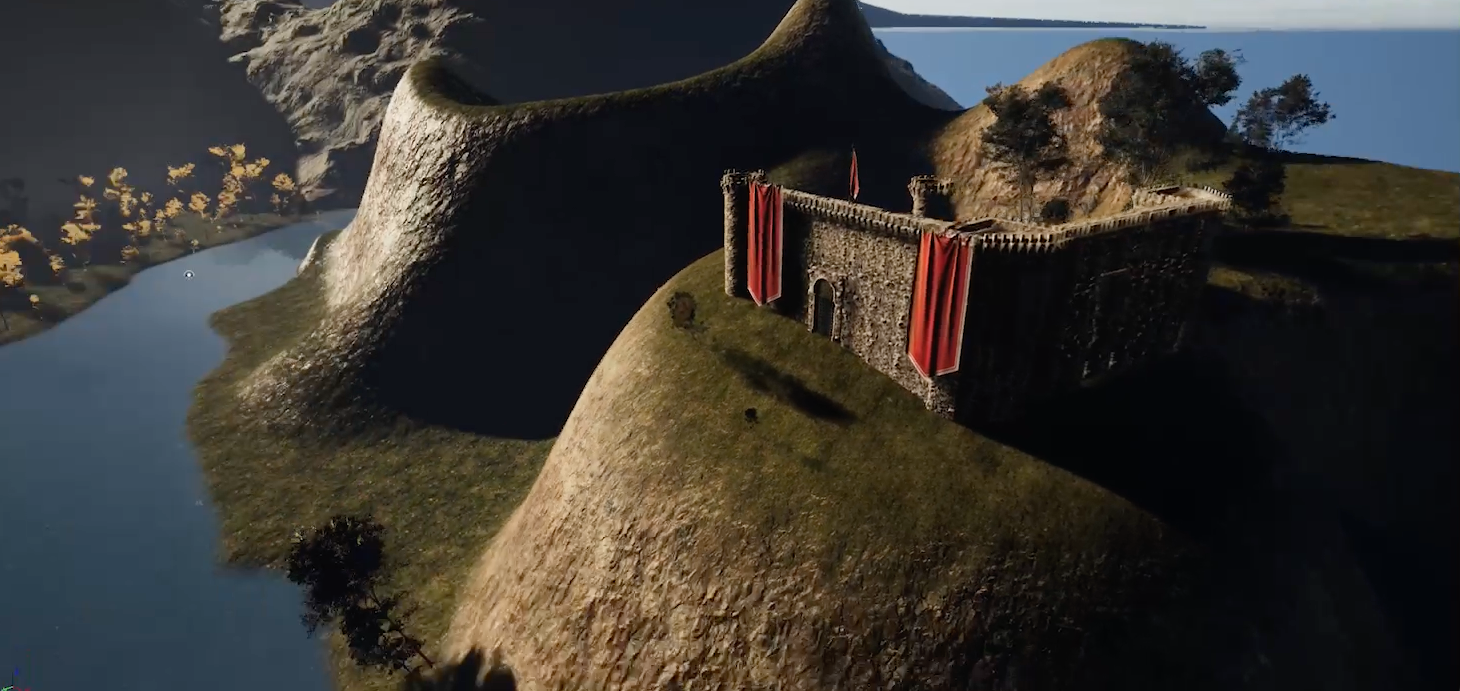
\includegraphics[width=\linewidth]{graphics/unreal-engine/Basics/Landscape-Castle.png}
    \caption{Tutorial Result: Castle.}
  \end{subfigure}
  \begin{subfigure}{0.45\textwidth}
    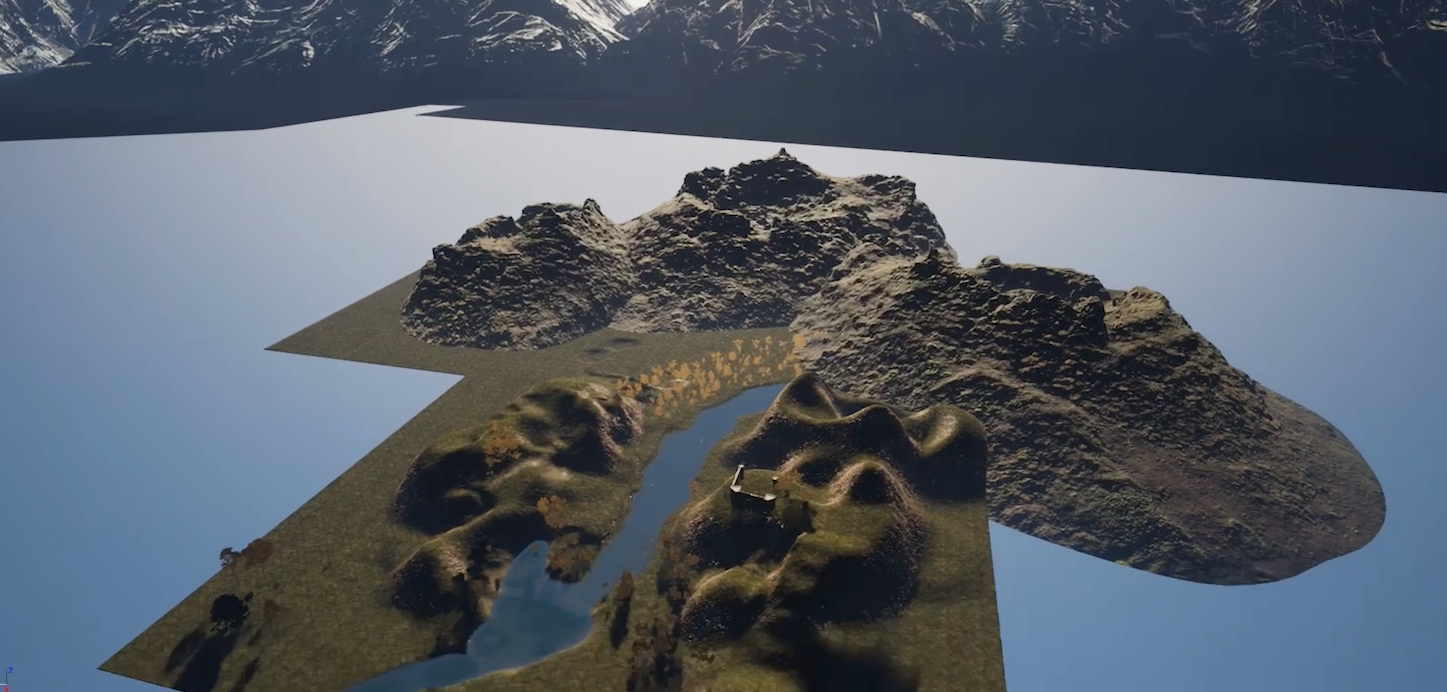
\includegraphics[width=\linewidth]{graphics/unreal-engine/Basics/Landscape-Overview.png}
    \caption{Tutorial Result: Landscape.}
  \end{subfigure}

  \begin{subfigure}{0.45\textwidth}
    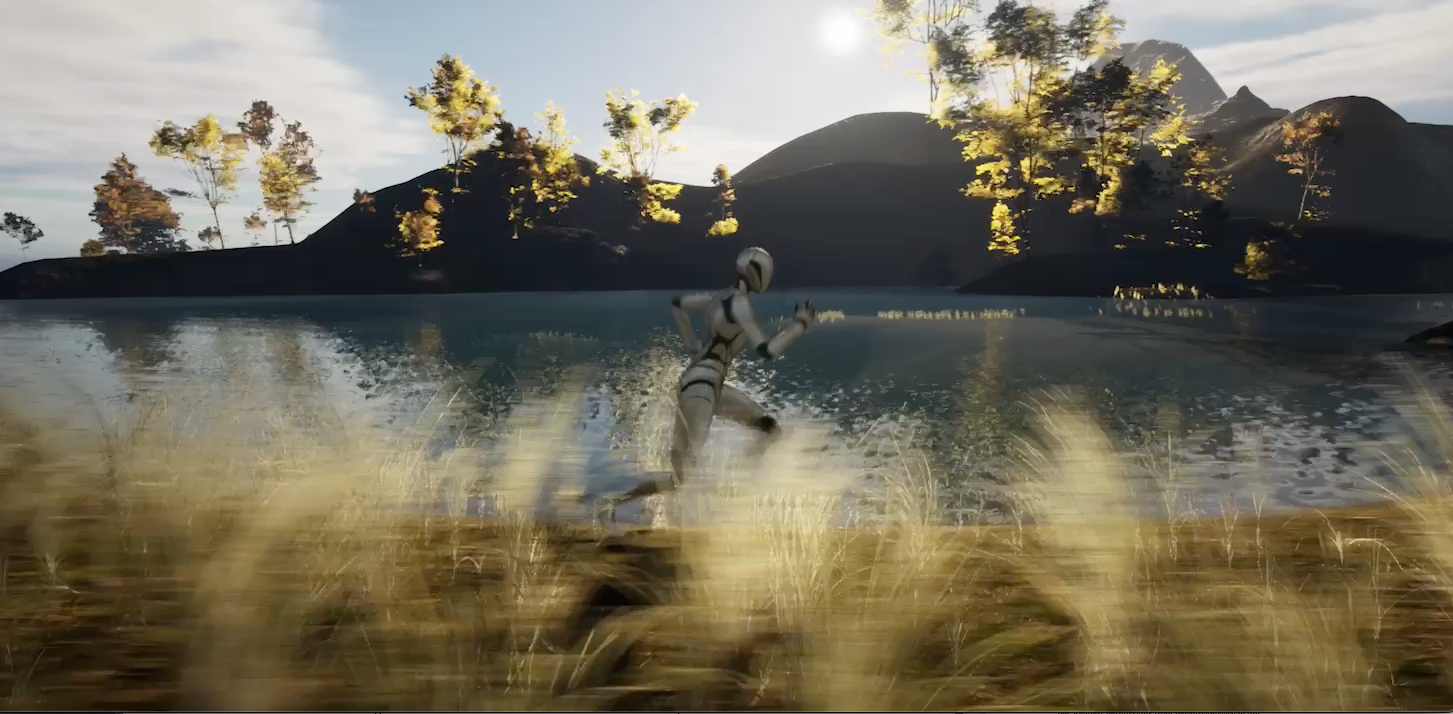
\includegraphics[width=\linewidth]{graphics/unreal-engine/Basics/Landscape-running.png}
    \caption{Tutorial Result: Character Running.}
  \end{subfigure}
  \begin{subfigure}{0.45\textwidth}
    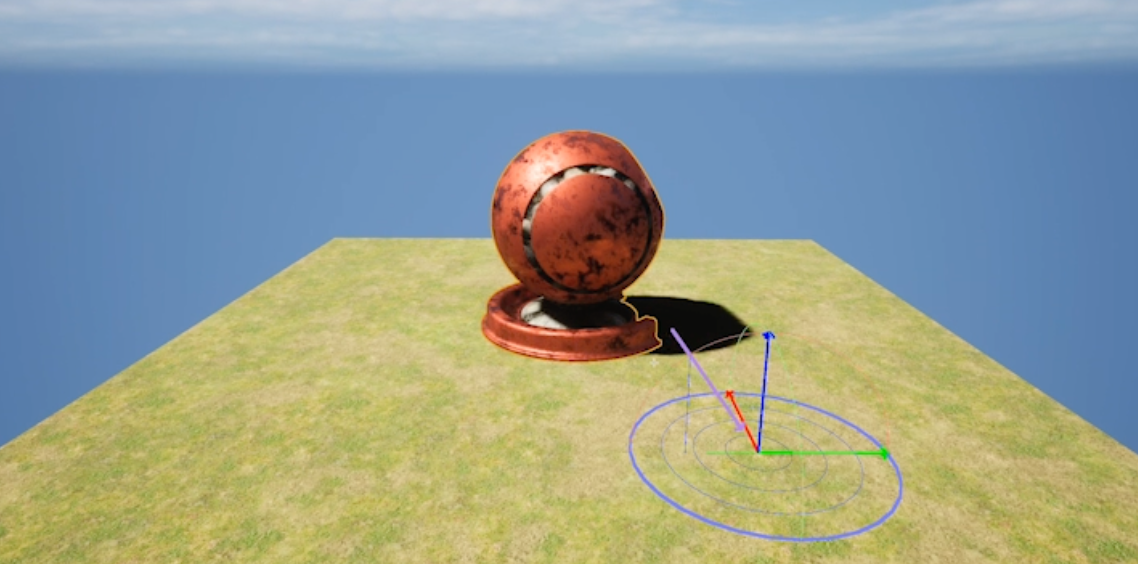
\includegraphics[width=\linewidth]{graphics/unreal-engine/Basics/Texture.png}
    \caption{Tutorial Result: Basic Texture.}
  \end{subfigure}
  \caption{Results from the First Tutorial.}
  \label{fig:ue-basic-tutorial}
\end{figure}

\subsection*{Studio Build}

As we just mentioned, modeling and texturing are extensive topics on their own. \gls{ue} excels at utilizing and rendering a wide range of objects, including a vast library of assets that can be used for free. Many of these assets are even scanned, providing incredible realism. However, when it comes to modeling custom objects, like the studio itself, achieving realism becomes much more challenging. Professional 3D artists would be required to achieve the desired level of accuracy and detail at this point. Nonetheless, it was fascinating to learn about the possibilities that \gls{ue} offers, even when relying solely on the engine itself. \\
We built the studio with very few elements (see Figure \ref{fig:ue-studio-build}): a shiny white floor for reflective lighting, a semicircle backdrop, the main anchorman desk, and some generic studio lights at the ceiling. Due to our lack of knowledge about modeling and texturing, it does not look very realistic, but the similarities to the real counterpart are clearly visible. We tried to at least create a realistic replica of the main desk using photogrammetry (Figure \ref{fig:photogrammetry-desk}), but it did not work as expected due to the semitransparent parts. As an alternative to photogrammetry, it would have been interesting to explore how \gls{nerf} or gaussian splatting would have performed in this domain, but due to time constraints, these methods could not be tested during the practical. It should be mentioned that \gls{genai} is becoming very useful in these domains, as \gls{sd} is already capable of creating 3D objects with ease. Therefore, modeling and texturing will very likely become much more accessible to semiprofessional and amateur users.

\begin{figure}[h]
  \centering
  \begin{subfigure}{0.45\textwidth}
    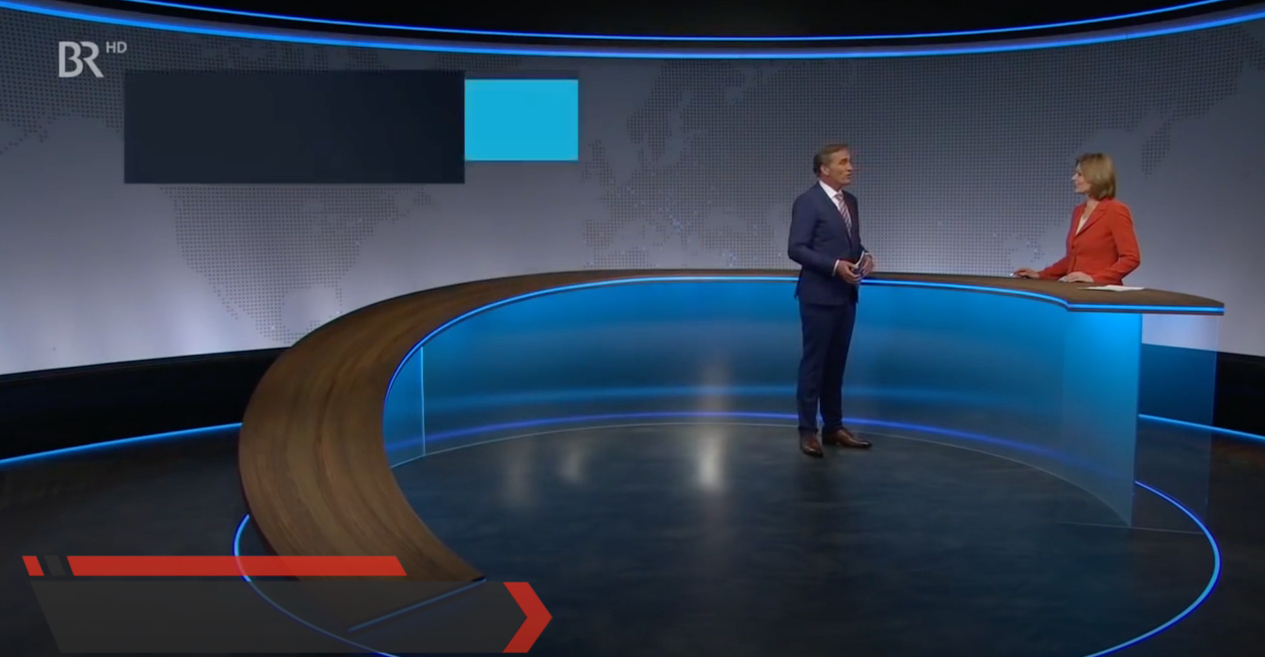
\includegraphics[width=\linewidth]{graphics/unreal-engine/studio/Studio-real.png}
    \caption{Real Studio for Comparison.}
  \end{subfigure}
  \begin{subfigure}{0.45\textwidth}
    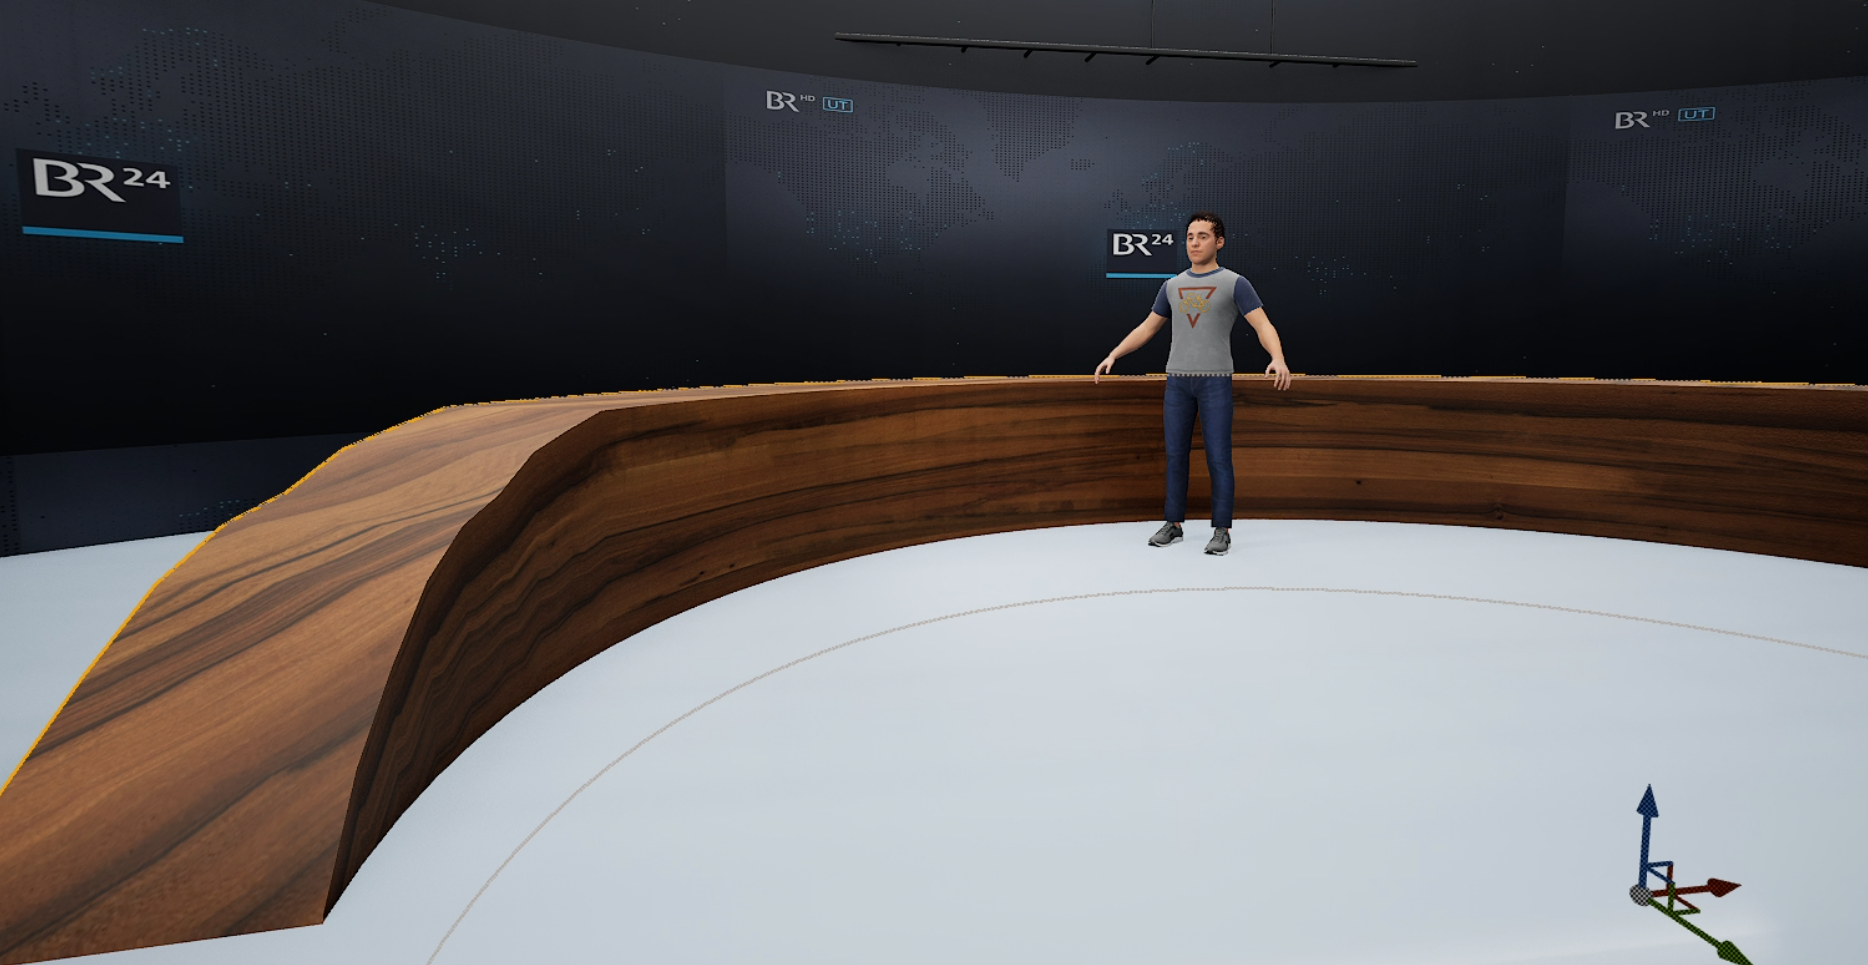
\includegraphics[width=\linewidth]{graphics/unreal-engine/studio/Studio-Comparison.png}
    \caption{Studio Recreation Modeled in \gls{ue}.}
  \end{subfigure}

  \begin{subfigure}{0.45\textwidth}
    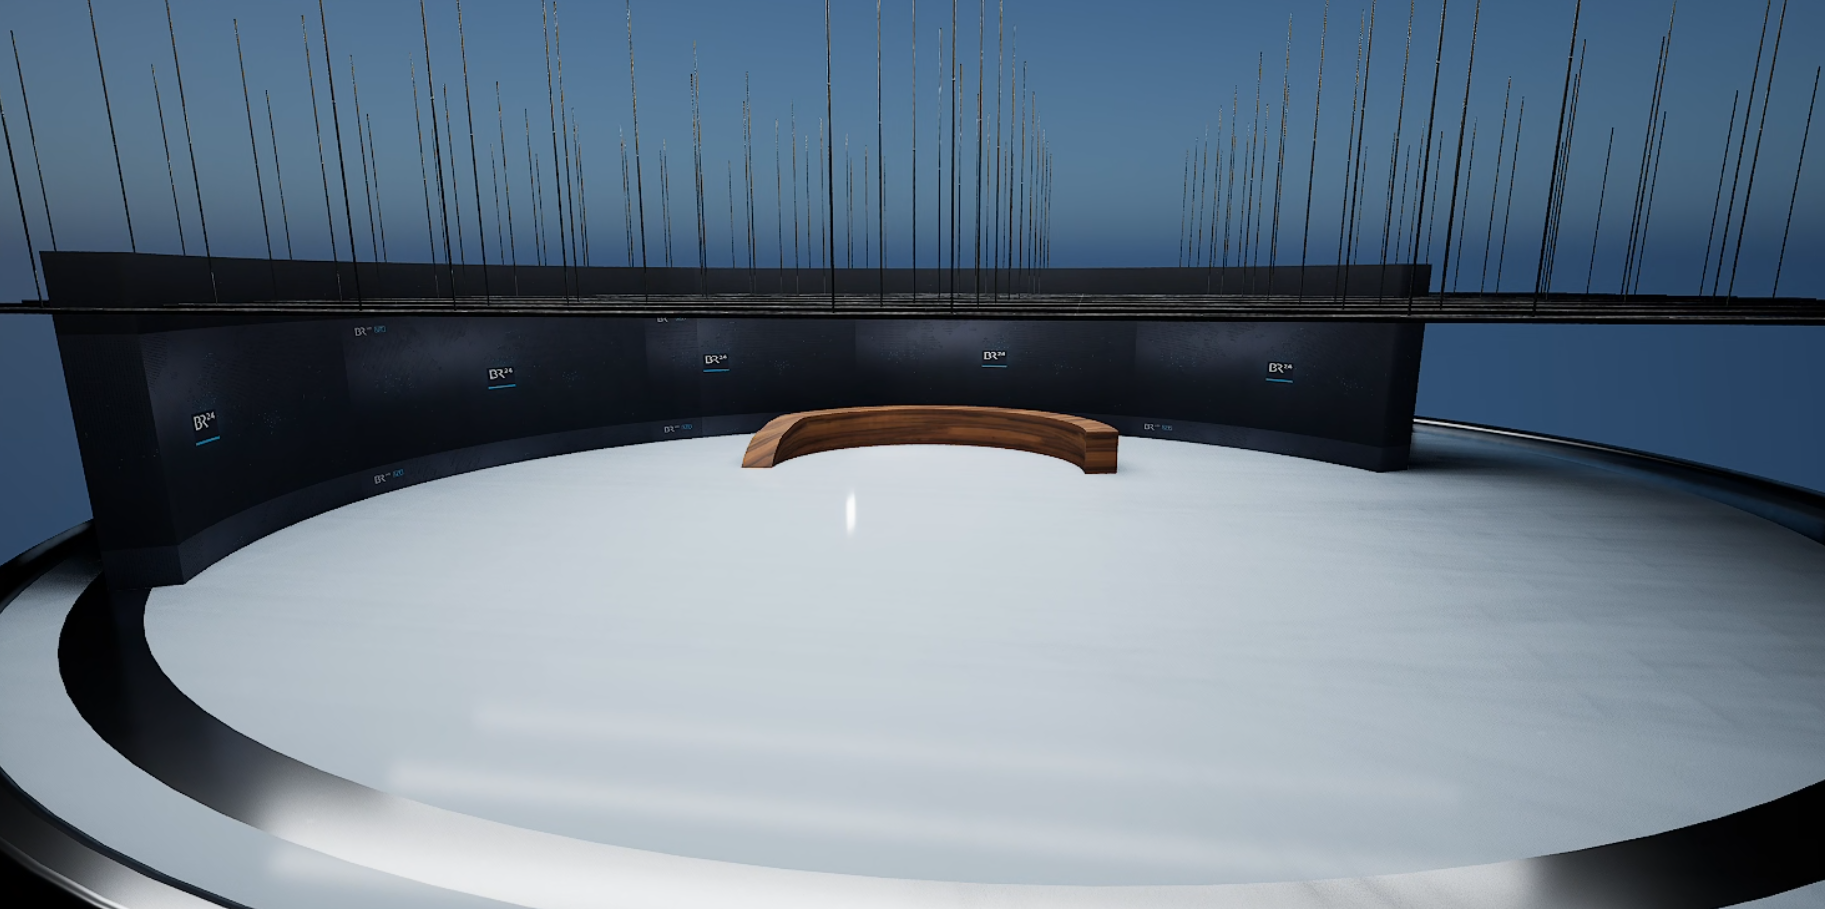
\includegraphics[width=\linewidth]{graphics/unreal-engine/studio/studio-totale.png}
    \caption{Studio Lighting.}
  \end{subfigure}
  \begin{subfigure}{0.45\textwidth}
    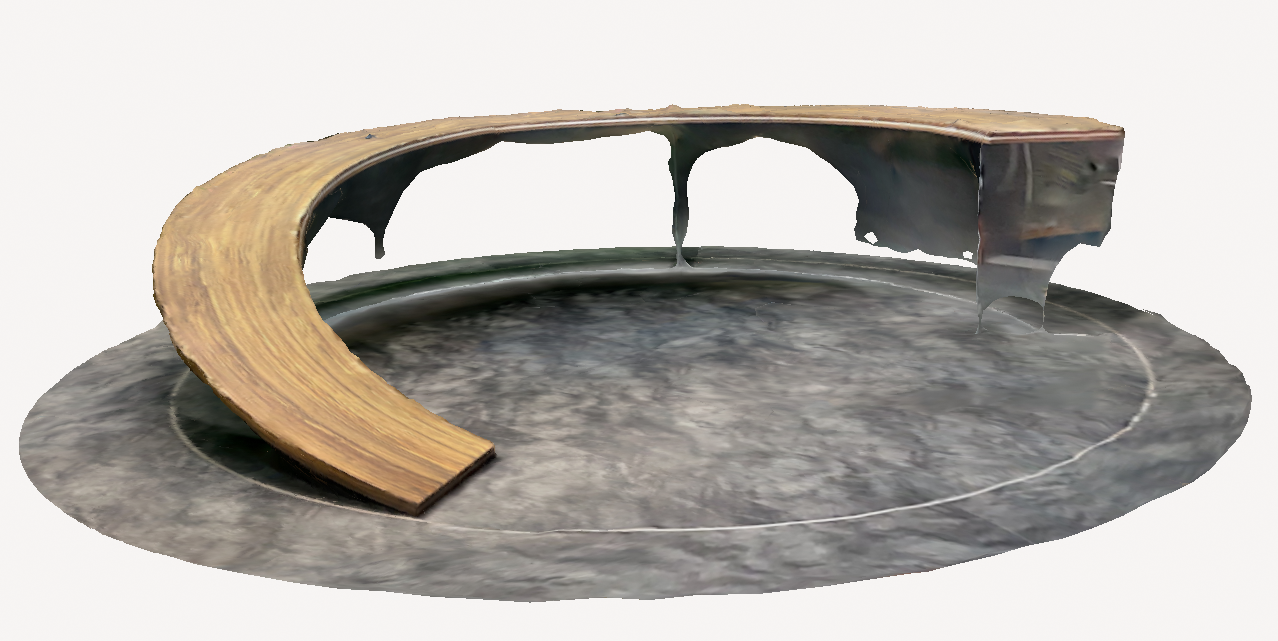
\includegraphics[width=\linewidth]{graphics/unreal-engine/studio/Photogrammetry-Desk.png}
    \caption{Photogrammetry Scan of the Desk.}
    \label{fig:photogrammetry-desk}
  \end{subfigure}
  \caption{Unreal Engine TV Studio Build.}
  \label{fig:ue-studio-build}
\end{figure}

\subsection*{Camera and Media Playback Logic} 

With the studio in place, a camera system needed to be implemented. \gls{ue} already provides support for cine cameras, which offer various settings reminiscent of their real-world counterparts, such as aperture, exposure, focal length, and focus. Initially, transitioning between cameras seemed straightforward using the integrated \textit{set view target with blend}. It was easy to set up multiple cameras within the scene and cut or animate between them using the mentioned method. This approach resembled the camera robots used in the real studio, utilizing easy-ease keyframes, which was advantageous. \\
However, there was a significant limitation with the existing method. While it effectively moved and rotated the view to the desired position, other parameters such as focal length, focus distance, and aperture did not change until the transition was complete. As a result, after the transition, these settings abruptly shifted, creating an undesirable visual effect. This behavior was unacceptable when aiming for smooth transitions. \\
To fix these issues, it was necessary to develop a separate camera system with custom control over the animation using \gls{ue}'s visual scripting language, \textit{Blueprint}. The scene now includes a master camera controlled by a Blueprint script (Figure \ref{fig:blueprint}). This Blueprint inherits methods for updating all relevant camera parameters, including a transition time that can be passed into the function call. 
\begin{figure}[h]
  \centering
  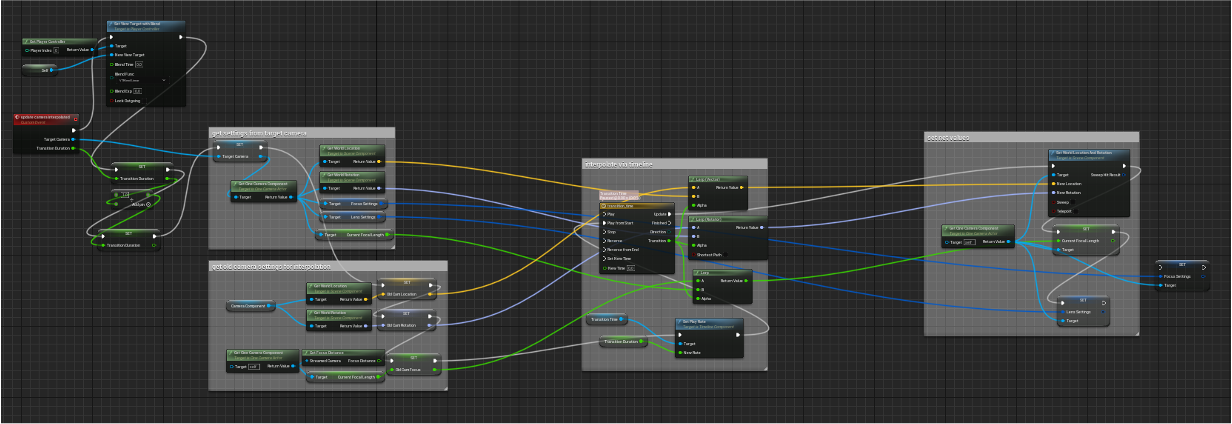
\includegraphics[width=1\textwidth]{graphics/unreal-engine/blueprint.png}
  \caption{Camera Blueprint.}
  \label{fig:blueprint}
\end{figure}
With the custom camera system in place, an endless number of cameras can be set up in the studio and the animated transitions follow automatically. Two examples of camera angles are depicted in Figure \ref{fig:cameras}.

\begin{figure}[h]
  \centering
  \begin{subfigure}{0.45\textwidth}
    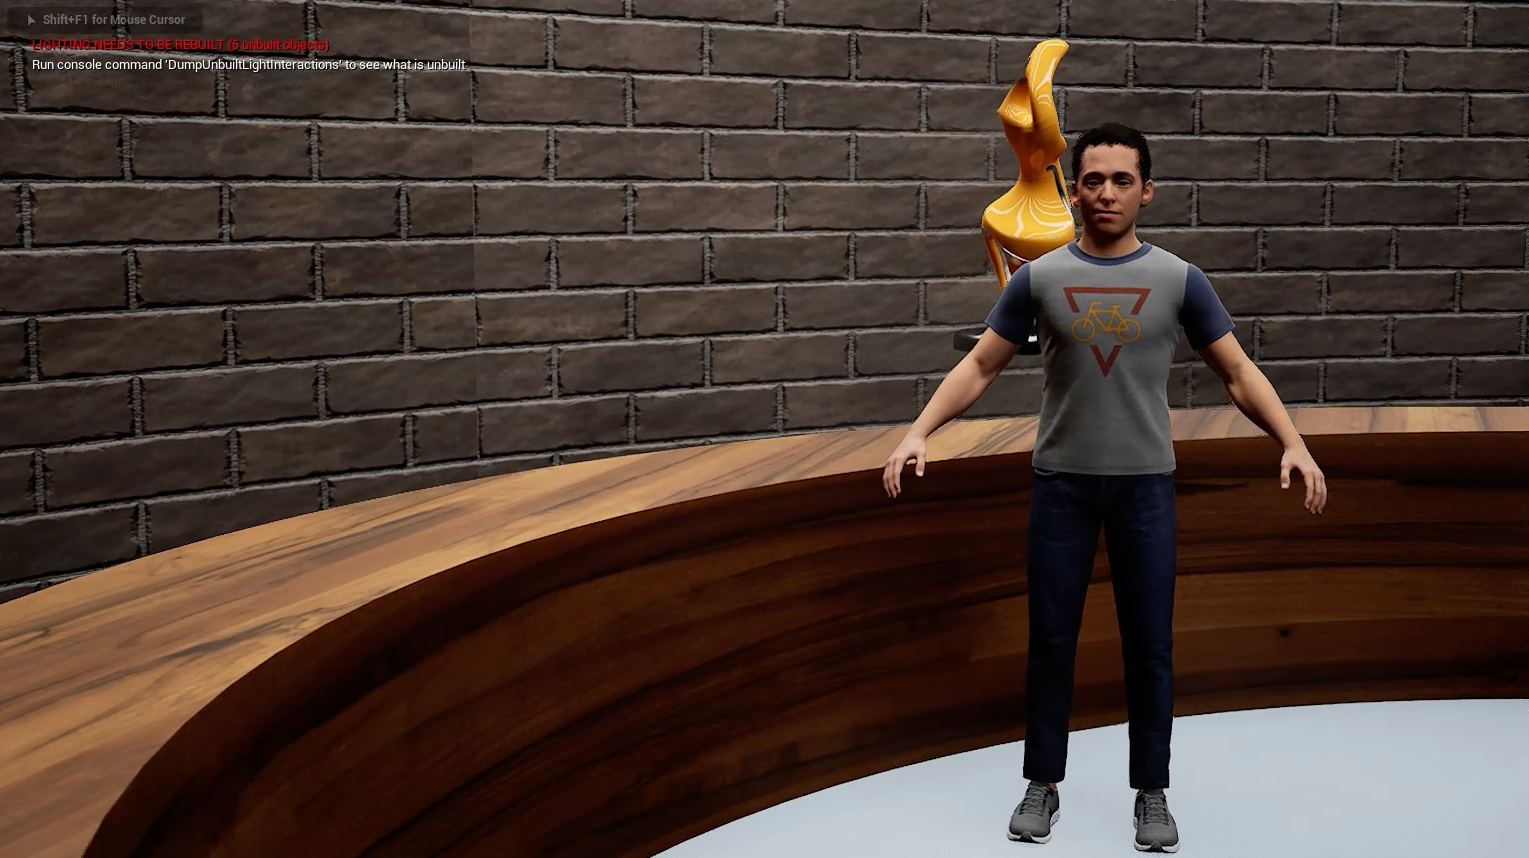
\includegraphics[width=\linewidth]{graphics/unreal-engine/camera angles/medium closeup.png}
    \caption{Medium Shot.}
  \end{subfigure}
  \begin{subfigure}{0.45\textwidth}
    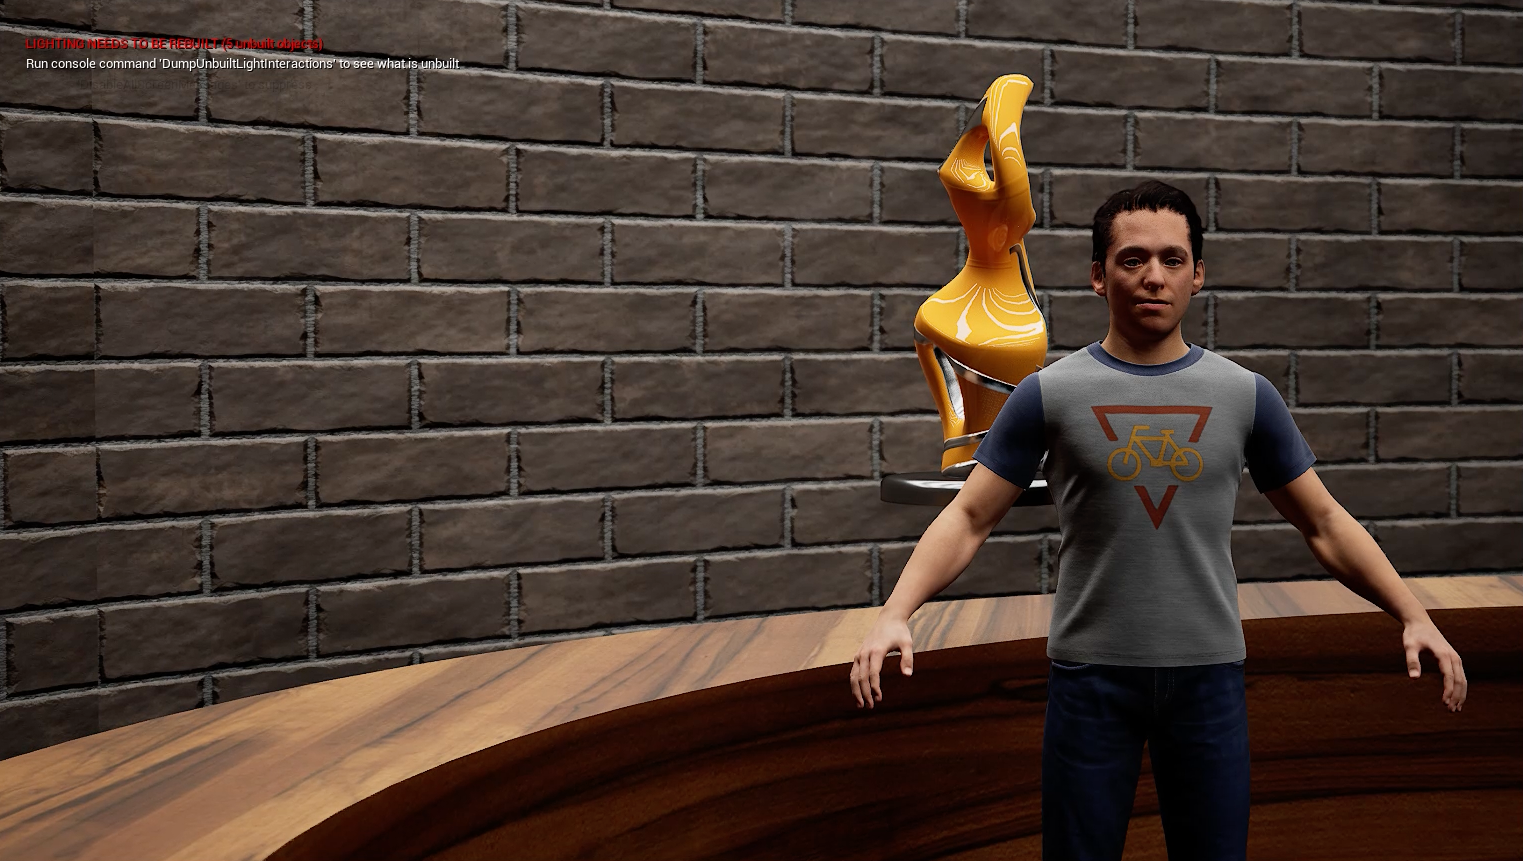
\includegraphics[width=\linewidth]{graphics/unreal-engine/camera angles/close up.png}
    \caption{Medium Close-Up.}
  \end{subfigure}
  \caption{Two Virtual Camera Examples in the Virtual Studio.}
  \label{fig:cameras}
\end{figure}

In many news formats, graphics presentations play a significant role. Analogously to the camera logic, we had to implement a Blueprint for the media playback in the background of the anchorman (see Figure \ref{fig:ue-media}). These presentations can be implemented in various ways, such as changing the background image or displaying a floating image next to the host. To better understand how \textit{BR24} accomplishes this, we spent time with video engineers on the show. The complexity of their system was overwhelming: \textit{BR24} has hundreds of templates for how hosts can present content, all rendered in real-time using a \textit{Viz.rt}graphics engine. \\
To keep the practical within a manageable scope, we decided to implement only one mockup display behind the news host, as depicted in Figure \ref{fig:ue-media}. The technical implementation of this feature is well documented in the \gls{ue} tutorials. It involves using a \textit{media player} feature that renders a material onto a plane mesh. We've briefly considered using separate software like \gls{obs} to render graphics but opted against it. Introducing another piece of software would have added complexity and reduced customizability. It would also have run against the idea of doing as much as possible inside UE. Like the camera system, additional functionality had to be added to the projection plane to use it in the desired manner. This was achieved by leveraging the knowledge gained from developing the camera system. Custom Blueprints were created to control the behavior of the projection plane and expose callable methods. This enabled control over parameters such as opacity, fade-in/out effects, loading and changing display images during runtime, and playing and pausing video media. \\
However, one issue remained with the projection plane: The images are not yet standardized, resulting in distortion. This will need to be addressed by applying appropriate adjustments to ensure that the images appear undistorted. Additionally, camera positions need to be set to ensure that the content in the background aligns appropriately with the projection.

\begin{figure}[h]
  \centering
  \begin{subfigure}{0.45\textwidth}
    \includegraphics[width=\linewidth]{graphics/unreal-engine/media/slide-real.png}
    \caption{Real Media Panel Reference.}
  \end{subfigure}
  \begin{subfigure}{0.45\textwidth}
    \includegraphics[width=\linewidth]{graphics/unreal-engine/media/slide-inplace.png}
    \caption{Virtual Media Panel in \gls{ue}.}
  \end{subfigure}
  \caption{Virtual Media Display.}
  \label{fig:ue-media}
\end{figure}

\subsection*{Character Build}
\gls{ue} provides its own toolset for creating comprehensive virtual characters, the so-called \textit{Metahuman} character creator, which facilitates character creation to some extent. Like \gls{ue}, the Metahuman creator facilitates quick results but has limitations to modeling and texturing customization options. To mitigate this problem, specialized software such as \textit{iClone Character Creator} or 3D animation software like \textit{Maya} or \textit{Blender} could be utilized. During the practical, these alternatives could not be covered, which is why we relied solely on \gls{ue}'s Metahuman editor. \\
Metahumans are currently undergoing active development and evolving rapidly. Editing Metahumans is done through a cloud-rendering web application in the browser, which is then synced to \gls{ue}. Creating a new character can be done from scratch or based on a real human; however, the method to achieve this changed over the course of several weeks, which shows the pace of development. In December 2023, \textit{gaussian avatars} became available for the first experimental implementation. This will drastically improve future workflows. \\
For our case, we initially had to employ a workflow called mesh-to-metahuman, which required a 3D mesh of a head to be imported into \gls{ue}. From there, it could be converted into a metahuman. We captured a head scan using the same photogrammetry workflow as with the studio table. The scan yielded exceptional results, as depicted in Figure \ref{fig:head-photogrammetry-scan}. Unfortunately, the resulting metahuman character did not bear much resemblance to the scan, as shown in Figure \ref{fig:metahuman-result}. With more expertise in character modeling, it may be possible to improve the likeness to a large extent. \\
During our research, \gls{ue} version 5.2 was released, introducing a new workflow that utilizes the faceID lidar sensors of an iPhone to capture facial performance data. The results were much better than with the mesh-to-metahuman workflow. Still, the Metahuman creator lacks customization options in various aspects, hindering us from achieving a higher likeness.

\subsection*{Character Animation}
Next, we needed to bring the character to life through animation. There were several options for achieving that objective, including using prerecorded performance data or implementing a live capture workflow. For the news format, a responsive and quick-to-produce approach was desirable, making the live version preferable. However, implementing a fully live capture system would require extensive tracking hardware, such as a full-body tracking suit. These suits can range in cost from €2,000 to €5,000 and can be complex to calibrate. Given the time constraints, a simpler and more cost-effective solution was chosen for the prototype. \\
Firstly, facial tracking was carried out using the iPhone's FaceID sensors. This allows for tracking of facial expressions and head rotation. Unreal Engine provides easy support for this, requiring only an iPhone on the same network as the Unreal PC and sometimes necessitating custom firewall settings. One challenge, however, is directing the gaze of the eyes towards a virtual camera. If the eyes do not look into the camera, the character can appear uncanny. 

\begin{figure}[h]
  \centering
  \includegraphics[width=0.5\textwidth]{graphics/unreal-engine/MH/bent-head.png}
  \caption{Uncanny Results from Our Animated Metahuman.}
  \label{fig:uncanny mh}
\end{figure}

Secondly, the rest of the body received an idle animation in the form of simple breathing. That way, the body looked more natural while the face was driven by an actor recording the moderation using the iPhone FaceID sensor. The result has room for improvement. Especially the face animations look quite uncanny (see Figure \ref{fig:uncanny mh}). The eyes do not look into the camera, and only a few facial landmarks are animated. This has to do with the technical limitations of the facial capture, as there are too few facial landmarks being tracked. \\
All in all, the performance falls deep into the uncanny valley.

\chapter{Study}
\label{chap:study}

During our research and work in the film and television industry, we have encountered various anecdotal assessments about trust in synthetic media. Due to the scarce research landscape on such a young topic, we decided to conduct our own exploratory study in the area of synthetic media trust and credibility. \\
As there are many different ways of creating synthetic media, we wanted to test multiple methods against each other and see how they performed. This resulted in our main research question (RQ1) about how the artificiality of synthetic media influences trustworthiness. Other questions in neighboring fields were postulated along the way.

\begin{table}[h]
  \centering
  \begin{tabularx}{\textwidth}{l|X}
    \textbf{Research Question} & \textbf{Description}\\
    \midrule
    RQ1a & Will video artificiality have an impact on trustworthines?  \\
    \midrule
    RQ1b & Does age, education or profession impact the effects in RQ1a?  \\
    \midrule
    RQ1c & What effect does the screen size have on the effects in RQ1a?  \\
    \midrule
    RQ2a & What effect does an AI logo label have?\\
    \midrule
    RQ2b & Does age, education, or profession impact the effects in RQ2?  \\
    \midrule
    RQ2c & What effect does screen size have on the effects in RQ2?  \\
  \end{tabularx}
  \caption{Research Questions}
  \label{tab:research-questions}
\end{table}

\section{Study Design}
\label{sec:study design}

Our goal was to find out more about the relationship between various types of synthetic media and their trustworthiness. In Chapter \ref{chap:background}, we discussed the relevant technologies we acquired over time. With access to these tools, we wanted to design a study that utilizes them in a practical scenario that is close to a daily practice use case. We therefore chose a TV newscast as a good testing environment. It provided sufficient control and the ability to experiment with \gls{tts}, \gls{v2v}, \gls{sd}, and even \gls{ue}. The newscast set the content. We chose to build upon existing news and not invent news in order to keep the content realistic. This should have eliminated bias towards unrealistic news, but we did not take into account differences in preexisting knowledge. We address this issue later while discussing the limitations (Section \ref{subsec:limitations}) of our study.

We decided to craft our study around the aforementioned spectrum of artificiality, as depicted in Figure \ref{fig:spectrum}. By introducing an increasing amount of synthetic media at each stage, we were hoping to measure the effects on trust. Artificiality, therefore, was one of our most important independent variables. Artificiality has close ties to the uncanny valley effect. Using several questions, we calculated a perceived index for each video. To avoid ambiguity with the term "AI", we named the index the \gls{ri} instead of "artificiality index". High \gls{ri} is analogous to low artificiality and a low uncanny valley effect. To ensure clear naming, we will refer to all these concepts only by the term \gls{ri} and avoid the other terms from now on.

We anticipated that the content itself would also have some effect on the judgements. To mitigate these issues, we created a second video at each quality level but filled it with different content. That way, we were able to control and compare results in both content groups. \\
Discussions about \gls{genai} led quickly to the call for marking footage that has been created with AI. We wanted to address this topic and decided to test for it as well. We did this by placing an AI logo in the upper corner of half the videos. The meaning of the AI logo was explained in advance. To be ethically correct, we informed the participants that the AI logo marks AI-generated content in some cases but can also be wrongly marked in other cases. While our study was already running, we discovered the paper by \citeauthor{toffTheyCouldJust2023}, in which the authors conducted similar testing in the domain of AI-generated texts. Unfortunately, we could not incorporate their findings to optimize our study design. However, since the AI marking experiment was just an add-on to our main research question, this was not too much of a missed opportunity. Please refer to Table \ref{tab:video-table} for a clear overview of the artificiality level, content, and AI logo marking strategy.

\begin{table}[h]
  \centering
  \begin{tabularx}{\linewidth}{c|c|X|X}
    \textbf{ID} & \textbf{AI Logo} & \textbf{Content} & \textbf{Artificiality}\\
    \midrule
    \href{https://drive.google.com/file/d/1wcgWiW07UWrh86xQaXqI0sc28WZoUlfj/view?usp=share_link}{1\_1} & \href{https://drive.google.com/file/d/1vB1aURRvoK19eWnzxmmBOS2HCp-MjvKG/view?usp=share_link}{in group B} & German unification day celebrations  & None: real video from broadcast \\
    \midrule
    \href{https://drive.google.com/file/d/1v2xDAOfhbPYudOGWFJGO_xGYwP5vcHD0/view?usp=share_link}{1\_2} & \href{https://drive.google.com/file/d/1eXjPoj32xWEWbeymlHlph6d1Er2pc0WT/view?usp=share_link}{in group A} & USA, McCarthy impeachment  & None: real video from broadcast \\
    \midrule
    \href{https://drive.google.com/file/d/1i9nGNuGLOpDQmDQ60ly6cXq_vwZerJUP/view?usp=sharing}{2\_1} & \href{https://drive.google.com/file/d/1MmLkxeuh8KvpInd3sAHWBUcjQTFfkLzo/view?usp=share_link}{in group B} & Smartphone usage decreased at Oktoberfest  & audio generated with \gls{v2v} conversion, video real+\gls{w2l} \\
    \midrule
    \href{https://drive.google.com/file/d/1uXVBxHgECmuQo0oYX_BEmDxBNMcCYRTt/view?usp=share_link}{2\_2} & \href{https://drive.google.com/file/d/1_XvS9ArS9ogeXNdpFXv_Y6kZvNhNbimM/view?usp=sharing}{in group A} & Introduction of new traffic management system  & audio generated with \gls{v2v} conversion, video real+\gls{w2l} \\
    \midrule
    \href{https://drive.google.com/file/d/1C62Fnwb2atoN66t6Bl5uo_RcMP1nEs04/view?usp=sharing}{3\_1} & \href{https://drive.google.com/file/d/1nlbBbndJvaUuxNYil-YdBl5RuEwqeZGO/view?usp=share_link}{in group B} & Youth music festival in Bavaria  & audio generated with \gls{tts}, video real + \gls{w2l} + style transformation with \gls{sd} \\
    \midrule
    \href{https://drive.google.com/file/d/193I_oJy46oyUWqAIpUUqwf0jJGURJfCH/view?usp=sharing}{3\_2} & \href{https://drive.google.com/file/d/1gN-h4__XSaG30pxgavr3Vki7do5z8Uzn/view?usp=sharing}{in group A} & US democratic party under pressure  & audio generated with \gls{tts}, video real + \gls{w2l} + style transformation with \gls{sd} \\
    \midrule
    \href{https://drive.google.com/file/d/1zpXDmkjIZmsndkNYb958O0d7xYyP-_Xg/view?usp=sharing}{4\_1} & \href{https://drive.google.com/file/d/1M8CdJttsTBFL8V8AzIyQ5oTx4RoZrxNi/view?usp=sharing}{in group B} & Robert Habeck visits Gamescom  & audio generated with \gls{v2v} conversion, video filmed in \gls{ue} \\
    \midrule
    \href{https://drive.google.com/file/d/1yeodhLKDHi1-bNLv5yvDVSv8_8UBqZIp/view?usp=sharing}{4\_2} & \href{https://drive.google.com/file/d/1JG3i8yMdtDclLWBPKXPJuKSw1i81NdKC/view?usp=sharing}{in Group A} & Biden visits middle east  & audio generated with \gls{v2v} conversion, video filmed in \gls{ue} \\
  \end{tabularx}
  \caption{Description of Our Test Videos.}
  \label{tab:video-table}
\end{table}

In total, there were eight videos, two for each of the four artificiality stages. In Group A, the second video was marked with the AI logo. Group B had it reversed, meaning the first video of each stage was marked. During interrogation, each participant was randomly assigned to group A or B. This measure was meant to compensate for side effects created by content and quality variations between the individual videos. The size of the groups was continuously balanced so that Groups A and B remained similarly sized. Within each group, the participants were presented with all eight videos, one after the other. The order of the videos was randomized for each participant in order to mitigate sequence bias. All questions regarding a specific video were answered alongside the concerned video, while no other video was present. This, in addition to the random sequence, was meant to reduce direct comparability effects. \\
In addition to the video questionnaire, we asked for basic demographic information. Our study encompasses both a between-subject design (A/B group division) and a within-subject design (analysis within Group A and B regarding age, device and occupation). However, the sample size within the groups was probably too small for certain tests.

\section{Procedure and Participants}
\label{sec:procedure-and-participants}

The study included an online questionnaire, conducted via the survey platform SoSci Survey, hosted by the \gls{lmu}. The survey was reachable via a single URL. The URL was spread among various media companies, university groups, and the author's personal contacts. After following the URL, a visitor was immediately assigned to group A or group B of the questionnaire. The survey itself was divided into three stages: 1) general and demographic questions, 2) main video evaluation, and 3) post-questionnaire evaluation and study explanations. During the second stage, all videos were presented to the participants in a randomized sequence. Along with each video, the participants had to answer five questions based on a Likert scale of 1 to 6.
\begin{enumerate}
  \item The content of this video is true.
  \item This video seems trustworthy.
  \item The anchorman is real.
  \item The anchorman's voice is real.
  \item The video has good quality.
\end{enumerate}
In addition to the Likert scale, the participants also had the opportunity to answer any of the questions with additional free-text remarks. During the post-questionnaire, we questioned how focused the participants were during the survey and how seriously they listened to the videos. On a scale of 1 to 3, we received a meaningless mean of 1.138 (closer to 1 is better) and a distraction mean of 1.318 (closer to 1 is better). On a four-step scale of how much the participants enjoyed the study (from \textit{not at all} to \textit{very much}) we received a mean of 3.185 (closer to 4 is better). According to these values, we infer that our gathered data accurately represents our participants' meaning and is not skewed by their unwillingness to participate. \\
After all the questions were answered, we provided an explanatory video for the study with a call to further spread the survey among friends and colleagues. We additionally incentivized participants to take part in the study by offering €50 to be given away in a lottery after the study was finished.
In total, we gathered \textit{N} = 195 valid participants. Regarding the age distribution (Figure \ref{fig:age-distribution}), the median lies at 30–34.

\begin{figure}[h]
  \centering
  \includegraphics[width=1\textwidth]{graphics/statistics/age-plot.png}
  \caption{Sample Age Distribution.}
  \label{fig:age-distribution}
\end{figure}
\begin{figure}[h]
  \centering
  \includegraphics[width=1\textwidth]{graphics/statistics/occupation.png}
  \caption{Sample Occupation Distribution.}
  \label{fig:occupation-plot}
\end{figure}

The distribution of industrial sectors shows a focus on IT (24.6\%) and creative media (39.5\%; Table \ref{fig:piechart-sectors}) while most participants were currently employed (50.3\%) or in education (28.2\%; Figure \ref{fig:occupation-plot}). 

\begin{figure}[h]
  \centering
  \begin{subfigure}{0.58\textwidth}
    \includegraphics[width=\linewidth]{graphics/statistics/piechart-sectors.png}
    \caption{Sample's Affiliation to Industry Sectors.}
    \label{fig:piechart-sectors}
  \end{subfigure}
  \begin{subfigure}{0.38\textwidth}
    \includegraphics[width=\linewidth]{graphics/statistics/piechart-devices.png}
    \caption{Distribution of Used Devices.}
    \label{fig:piechart-devices}
  \end{subfigure}
  \caption{Industry Sectors and Used Devices.}
\end{figure}

We also collected data about the last educational institution attended, gender, and country, but these factors had no relevant effects and thus could be omitted. A better independent variable for such effects would have been to gauge AI/ and media-literacy, a factor we strongly recommend for future studies. Regarding display devices, smartphones, laptop monitors, and larger external monitors were quite evenly distributed (compare Figure \ref{fig:piechart-devices}). We compare this self-assessment with our measurements later on. Lastly, we asked participants which of the factors (video content, video quality, or AI logo) had the strongest influence on their judgments regarding perceived trustworthiness (see Figure \ref{fig:most-influence}).

\section{Results}
\label{sec:results}

Before we discuss further analysis, we want to address the topic of handling our Likert scales. We are aware of the ongoing discussion about whether Likert scales can produce and be interpreted as metric data or if they can only supply ordinal data. The central argument is that equidistance between the options cannot be ensured. Devaluing these scales to ordinal data would prohibit arithmetic operations with the values as well as many statistical tests. Many Likert scales use four items, and there are recommendations to increase the number of Likert scale points to make them closer to continuous scales and normality \cite{wuCanLikertScales2017a}. We complied by using six points instead of four. In our next research, we will most likely use 10 or 11 points, as suggested by \Citet{hodgePhraseCompletionScales2007}. We further assume our Likert measurements to be metric; however, we checked some parametric tests with their nonparametric counterparts to ensure they would not deliver drastically different results regarding significance. In all of the conducted statistical tests, this was never the case.

\subsection{Measuring Artificiality}

As mentioned in the study design, we wanted to measure the perceived artificiality to confirm that our design of the artificiality spectrum was right. We did this by asking whether the anchorman's voice was true and then calculating the mean of the two values. As mentioned earlier, we further refer to this as the \gls{ri}. \\
The mean values (Table \ref{tab:RIs-mean}) show that our artificiality spectrum worked almost as intended. We initially assumed that the \gls{ue} example (cases 4\_* in Table \ref{tab:video-table}) would rank last because it looked the most uncanny. But instead, the perceived \gls{ri} shows that, in fact, the \gls{ue} videos ranked third, while the \gls{sd} videos from group 3\_* ranked last (Figure \ref{fig:spectrum}). The reason for our misjudgment is clear. We thought the uncanny character of the \gls{ue} example would have the most influence, but actually the very synthetic-sounding voice of the 3\_* videos reduced the \gls{ri} strongly. To make matters worse, 3\_* videos were altered using \gls{sd}, which made them even more artificial. In summary, these videos felt less good compared to the 4\_* videos.

\begin{table}[h]
	\centering
	\caption{Realism Index' Mean Value Ranking.}
	\label{tab:RIs-mean}
	{
		\begin{tabular}{lrrrrrrrrrr}
			\toprule
			 & 1\_1 & 1\_2 & 2\_1 & 2\_2 & 4\_1 & 4\_2 & 3\_1 & 3\_2 & *\_1 & *\_2 \\
			\cmidrule[0.4pt]{1-11}
			Mean & $5.39$ & $5.38$ & $2.7$ & $3.28$ & $1.92$ & $2.09$ & $1.64$ & $1.54$  & $2.93$ & $3.07$\\
			\bottomrule
		\end{tabular}
	}
\end{table}
\begin{figure}[h]
  \includegraphics[width=1\textwidth]{graphics/statistics/RIs/RI_compilation.png}
  \caption{Distribution of Realism Indexes: Individual Videos and Grouped.}
  \label{fig:all-RIs}
\end{figure}

Figure \ref{fig:all-RIs} plots the \gls{ri}s for each video across both subgroups (A and B). \\
It lies in the nature of the questions that the resulting \gls{ri} data is heavily skewed in many cases (figures in Section \ref{fig:all-RIs}). Naturally, we assume that most people will regard something as real if it is real. This would usually prohibit the assumption of normality. To mitigate that, we combined all \gls{ri}s for videos *\_1 and *\_2 and cross-checked some tests with this combined distribution. As seen in Figure \ref{fig:all-RIs}, they can be considered to be normally distributed. Shapiro-Wilk tests deliver p-values of 0.31 for \gls{ri} *\_1 and 0.024 for \gls{ri} *\_2, while all other non-grouped \gls{ri}s have p-values of < 0.001. In addition, the central limit theorem for larger sample sizes (n > 30) considers normality to be less critical. With our sample size of 195, we continue using parametric tests on all \gls{ri} values.

\subsection{RQ1: Artificiality and Trust Relationship}
\label{subsec:RQ1}

Tables \ref{tab:trust-RI1-correlations} and \ref{tab:trust-RI2-correlations} show a significant positive correlation in each of the expected cases, while the correlation strengths cover everything from weak (r = 0.251) to strong (r = 0.617). Therefore, we can confirm Hypothesis H1a. \\
One lesson for media companies from this could be that the highest possible quality should be strived for before such content goes online to ensure the highest trust ratings. However, we must keep in mind that the tests only cover subject testing. As every participant has seen all of the contents, even in random order, they are clearly influenced by having the other videos for reference. It might be interesting to conduct further studies with isolated groups, where only one level of quality is tested. It might be possible that artificial-looking content could score similar trust results as realistic content when there is no comparison in the participant's frame of reference.

\begin{table}[h]
	\centering
	\caption{Pearson's r Correlations trust - RIs 1.}
	\label{tab:trust-RI1-correlations}
	{
		\begin{tabular}{lrrrrr}
			\toprule
			Variable &  & 1\_1\_trust & 2\_1\_trust & 4\_1\_trust & 3\_1\_trust  \\
			\cmidrule[0.4pt]{1-6}
			1\_1\_RI & Pearson's r & \textbf{0.617} & $0.006$ & $0.022$ & $0.080$  \\
			$$ & p-value & \textbf{$<$ .001} & $0.931$ & $0.756$ & $0.264$ \\
			2\_1\_RI & Pearson's r & $0.107$ & \textbf{0.444} & $0.153$ & $0.224$ \\
			$$ & p-value & $0.135$ & \textbf{$<$ .001} & $0.032$ & $0.002$\\
			4\_1\_RI & Pearson's r & $\approx 0$ & $0.081$ & \textbf{0.312} & $0.263$   \\
			$$ & p-value & $0.990$ & $0.259$ & \textbf{$<$ .001} & $<$ .001 \\
			3\_1\_RI & Pearson's r & $0.168$ & $0.053$ & $0.132$ & \textbf{0.256} \\
			$$ & p-value & $0.019$ & $0.466$ & $0.066$ & \textbf{$<$ .001} \\
			\bottomrule
			% \addlinespace[1ex]
			% \multicolumn{10}{p{0.5\linewidth}}{* p $<$ .05, ** p < .01, *** p < .001} \\
			% \multicolumn{10}{p{0.5\linewidth}}{* $$} \\
			% \multicolumn{10}{p{0.5\linewidth}}{*** $$} \\
			% \multicolumn{10}{p{0.5\linewidth}}{** $$} \\
		\end{tabular}
	}
\end{table}
\begin{table}[h]
	\centering
	\caption{Pearson's r Correlations trust - RIs 2.}
	\label{tab:trust-RI2-correlations}
	{
		\begin{tabular}{lrrrrr}
			\toprule
			Variable &  & 1\_2\_trust & 2\_2\_trust & 4\_2\_trust & 3\_2\_trust  \\
			\cmidrule[0.4pt]{1-6}
			1\_2\_RI & Pearson's r & \textbf{0.598} & $0.109$ & $0.103$ & $0.009$  \\
			$$ & p-value & \textbf{$<$ .001} & $0.065$ & $0.076$ & $0.448$ \\
			2\_2\_RI & Pearson's r & $0.051$ & \textbf{0.606} & $0.197$ & $0.174$ \\
			$$ & p-value & $0.238$ & \textbf{$<$ .001} & $0.003$ & $0.007$ \\
			4\_2\_RI & Pearson's r & $0.014$ & $0.009$ & \textbf{0.300} & $0.003$   \\
			$$ & p-value & $0.990$ & $0.259$ & \textbf{$<$ .001} & $<$ .001 \\
			3\_2\_RI & Pearson's r & $0.024$ & $0.043$ & $0.128$ & \textbf{0.251} \\
			$$ & p-value & $0.369$ & $0.273$ & $0.037$ & \textbf{$<$ .001} \\
			\bottomrule
			% \addlinespace[1ex]
			% \multicolumn{10}{p{0.5\linewidth}}{* p $<$ .05, ** p < .01, *** p < .001} \\
			% \multicolumn{10}{p{0.5\linewidth}}{* $$} \\
			% \multicolumn{10}{p{0.5\linewidth}}{*** $$} \\
			% \multicolumn{10}{p{0.5\linewidth}}{** $$} \\
		\end{tabular}
	}
\end{table}

As for Research Question RQ1b, we could not find any significant differences comparing groupings by age, education, or profession. Conducting MANOVA tests by age as the fixed factor delivered hints of significant differences (p-value = 0.005), but a more detailed look using ANOVA did not show any significance. This is most likely due to the small sample sizes after division into subgroups. \\
Creating subgroups by education or profession causes even smaller subgroups, which is why many calculations could not be performed properly. Furthermore, there are many disturbances that clearly overshadow any effect caused by age, education, or profession differences. To summarize, we can state that there are differences between the subgroups overall, but we cannot reliably say where and in which direction. Additionally, the significance quickly disappears in our data. It is very clear that an isolated study would be needed to target these sorts of questions, of which our exploratory study found hints.

By reading through some of the comments on our study and talking informally with subjects, we gained the feeling that display size could have some impact on the results. Logically, a smaller screen would make visual imperfections less visible, resulting in better \gls{ri}s for a given video. While testing for RQ2c (Does screen size have an effect on the Ris?), we can state similar findings as for RQ1b: Using the MANOVA, we can state that there are differences (p-value = 0.039) in \gls{ri}s considering the used devices. \\
In ANOVA tests, only one of the cases was significant (2\_2\_RI: p-value = 0.024). Post hoc analysis showed only one significant case: smartphone vs. laptop, with a mean difference of +0.719 and a p-value of 0.02. This would support our assumption that a smaller display causes a (very) slightly higher \gls{ri}. \\
We do not think this one result represents any convincing evidence, as all other cases are insignificant, but together with the verbal discussion, we still believe there are hints that this topic could be researched further, especially with media consumption on mobile devices becoming more and more prevalent.

\subsection{RQ2: Effects of AI Disclosure to Trust}
\label{subsec:RQ2}

\begin{figure}[h]
  \centering
  \includegraphics[width=.5\textwidth]{graphics/statistics/most-influence.png}
  \caption{Sample's Judgment Regarding the Most Influential Trust Factors.}
  \label{fig:most-influence}
\end{figure}

We wanted to get an understanding of what effect the disclosure of a possibly AI-generated video might have. A first self-assessment by the participants implies that there is a very minor effect of the markings (compare Figure \ref{fig:most-influence}). As mentioned in Section \ref{sec:rel-studypart}, \Citeauthor{toffTheyCouldJust2023} discovered a statistically significant reduction in perceived trustworthiness, perceived accuracy, and perceived fairness. \\
Their study observed AI-generated texts, which are much more controllable than audio-visual content. Still, we were interested in comparing our results with theirs. \\
Before examining our data, we crafted two working theories about what we would expect to measure. The theories were based on previous testing, anecdotes, and assessments by various parties. We expected to see a drop in perceived trust in good-quality videos (1\_* and 2\_* videos) but an increase with bad-looking examples (4\_* and 3\_* videos). Our expectations followed a certain logic:

(1) Convincing-looking videos, once marked as AI-generated, would decrease due to present prejudices about AI. Fears about an unrecognized deepfake would fuel such thoughts. \\
(2) On the other hand, bad-looking videos would have a low trust value as a starting point, which we confirmed with RQ1. Once such a video is revealed as AI-marked, a viewer will accept its inferior quality because the reason for the inferiority is now clear. An effect as in (1) would not appear because the content had bad quality in the first place. A rather contrary, relieved feeling would be expected, as the presented AI is "just not good" and therefore less scary than in the first scenario. Clearly, both scenarios are speculations or, at best, educated guesses. It is questionable, given the design of the study, if any significance can be measured in the presence of many other disruptive factors.

As for the statistical evaluation, we conducted Student's t-tests and Mann-Whitney U-tests in case the normality of our data were to be questioned. The dependent variables were the \gls{ri} values, grouped by condition, whether a particular video was marked or not. Grouped \gls{ri}s (*\_1 and *\_2) are the same accumulated, normally distributed values as introduced in Figure \ref{fig:all-RIs}. Unfortunately, we could not measure any significance in any of the categories (compare with Table \ref{tab:ttest_logo-trust}). With our study design, which was focused on measuring the overall effects of increasing artificiality, this was to be expected.

\begin{table}[h]
	\centering
	\caption{AI Markings: T-Test/U-Test.}
	\label{tab:ttest_logo-trust}
	{
		\begin{tabular}{lrr|lrr}
			\toprule
			\textbf{Case} & \textbf{p (t-test)} & \textbf{p (u-test)} & \textbf{Case} & \textbf{p (t-test)} & \textbf{p (u-test)}  \\
			\cmidrule[0.4pt]{1-6}
			1\_1\_trust & $0.091$ & $0.137$ & 1\_2\_trust & $0.487$ & $0.397$ \\
			2\_1\_trust & $0.390$ & $0.417$ & 2\_2\_trust & $0.481$ & $0.465$ \\
			3\_1\_trust & $0.771$ & $0.588$ & 3\_2\_trust & $0.983$ & $0.737$ \\
			4\_1\_trust & $0.698$ & $0.512$ & 4\_2\_trust & $0.152$ & $0.077$ \\
			grouped RI *\_1 & $0.800$ & $0.788$ & grouped RI *\_2 & $0.753$ & $0.735$\\
			\bottomrule
			% \addlinespace[1ex]
			% \multicolumn{4}{p{0.5\linewidth}}{\textit{Note.} Student's t-test.} \\
			% \multicolumn{4}{p{0.5\linewidth}}{$^{0}$ Brown-Forsythe test is significant (p $<$ .05), suggesting a violation of the equal variance assumption} \\
		\end{tabular}
	}
\end{table}

This shows that the varying video quality and content have too strong effects, overshadowing any effects an AI marking could have. We therefore cannot confirm nor deny the results from \Citeauthor{toffTheyCouldJust2023}. By examining comments, we also determined that we had created some differences between videos of one quality stage by having chosen differing topics or fields on the content side. The choices of content should have been made more neutral, or at least more similar, within one quality stage. \\
In a follow-up study where this has been improved, it might be easier to measure the effects of the AI logo. Like \Citeauthor{toffTheyCouldJust2023}'s study, the groups between marked and unmarked must be comparable in both dimensions, quality and content.

We can conclude that the participants' self-assessment, depicted in Figure \ref{fig:most-influence}, seems to be accurate. We cannot measure any significant effects regarding the AI mark, as the other variables introduce too many disturbances. Regarding the direction of the effects, it is also impossible to state anything robust. Judging by our experiences, we are still not ready to omit our aforementioned working theories, but for further research in this direction, a different study design would be required.

 \subsection{Exploratory Factor Analysis}
\label{subsec:factor-analysis}

To further inspect the quality of our questionnaire, we conducted an exploratory factor analysis (Table \ref{tab:factorLoadings}) for our main questions. The results show that all measurements somewhat point to the same latent variable. This surely conforms to the correlations we found in the previous sections. Even if the questions all point towards the same measurement, they are interesting to us because all of the variables could potentially be manipulated in a follow-up study.

\begin{table}[h]
	\centering
	\caption{Factor Loadings.}
	\label{tab:factorLoadings}
	{
		\begin{tabular}{lrr}
			\toprule
			Variable & Factor 1 (latent variable)  \\
			\cmidrule[0.4pt]{1-2}
			all seems-trustworthy & $0.900$  \\
			all video-quality is-good & $0.735$  \\
			all moderator is-real & $0.606$  \\
			all content is-true & $0.589$  \\
			all voice is-real & $0.560$  \\
			\bottomrule
			% \addlinespace[1ex]
			% \multicolumn{3}{p{0.5\linewidth}}{\textit{Note.} Applied rotation method is promax.} \\
		\end{tabular}
	}
\end{table}

\subsection{Discussion}

This study's exploration into the impact of synthetic media's artificiality on trustworthiness has yielded significant insights while also opening avenues for future research.

\subsubsection{Impact of Artificiality on Trustworthiness}
The findings indicate a clear correlation between the artificiality of synthetic media and its perceived trustworthiness. This supports the hypothesis that higher artificiality negatively impacts trust. Through statistical analysis, particularly using Pearson's r correlations, a clear and consistent correlation was identified: as the degree of artificiality in synthetic media increases, its perceived trustworthiness decreases. This trend was most evident in the calculated \gls{ri} values, where videos with higher \gls{ri}s, indicating lower artificiality, were consistently deemed more trustworthy by participants. \\
This pattern held across various forms of synthetic media, encompassing different alterations such as \gls{v2v} conversion, \gls{tts}, \gls{sd} and \gls{ue}. Each form of synthetic media exhibited a distinct impact on trust, underscoring the complexity of how artificiality is perceived in different media contexts. The study's findings also highlight the significant role of both visual and auditory elements in shaping perceptions of artificiality. The synthetic voices, in particular, in \gls{tts} and \gls{v2v} conversions, emerged as a crucial factor affecting trustworthiness ratings, whereas the inferior \gls{tts} always led to worse results than \gls{v2v} samples. \\
However, it is important to note that while the correlation between artificiality and trustworthiness was clear, the study's design may have limitations in capturing finer variations in trustworthiness at different artificiality levels.

\subsubsection{Demographic Factors and Screen Size}
Notably, the research did not find significant effects based on demographics such as age, education, or profession. The study's sample, while diverse, might not have been sufficiently large or varied to detect subtle demographic differences in perception. This aspect of the research, while not conclusive, opens up interesting directions for future investigations. \\
Another intriguing aspect of the study was the exploration of the influence of screen size on the perception of synthetic media. While the results regarding screen size were statistically inconclusive, they hint at an underlying dynamic worth investigating. The hypothesis was that smaller screens might mask imperfections in synthetic media, potentially leading to higher trust ratings. This aspect of the research, though not definitively proven, suggests that the medium through which synthetic media is consumed – whether it be a smartphone, laptop, or larger display – could subtly influence how viewers perceive its authenticity and trustworthiness. \\
The implication of these findings, particularly regarding screen size, is noteworthy. In an era where media consumption varies widely across devices with different screen sizes, understanding how this variable affects perception could have significant implications for the design and dissemination of synthetic media. Future studies, therefore, should consider incorporating a more focused examination of screen size as a variable, potentially revealing more about how the context of media consumption impacts viewer perception and trust.

\subsubsection{Influence of Disclosing the AI-Generated Nature of Content}
The absence of a significant impact from AI logo branding on trust contradicts some existing narratives around AI transparency, like the works of \Citeauthor{toffTheyCouldJust2023}. In relation to our study, this indicates that viewer perceptions are more influenced by the content and presentation of the media than by disclaimers or labels (refer to Section \ref{subsec:RQ2}). In discussions with participants, as well as the free-text submissions, we received feedback that some videos were not believed and therefore decreased their trust ratings. One example was the report about German minister Robert Habeck visiting the GamesCom convention (video 4\_1, Figure \ref{tab:video-table}). This event actually happened but was frequently evaluated as fake. The influence of the quality of the videos was also often addressed by participants. This applied not only to bad video and audio quality but also to cases, where participants recognized the actual speakers' voice in the \gls{v2v}-converted audios. Apparently, this broke their illusion and therefore lowered the trust ratings. \\
This finding suggests that the factors influencing viewer perceptions of synthetic media might be more complex than we assumed. It appears that the content itself and its presentation hold more sway over viewers' trust than the mere presence of disclaimers or labels indicating AI involvement. This could imply that viewers are either not significantly influenced by such labels or that the quality and nature of the content overshadow any concerns raised by the knowledge of AI involvement. The absence of a significant difference in trustworthiness between AI-labeled and unlabeled content could also point to a potential desensitization among viewers to AI-generated content, as it becomes more prevalent in the media landscape. Alternatively, it could indicate a baseline level of trust or skepticism that is not easily swayed by labeling. \\
These insights open up new ideas for research, particularly in understanding how transparency about AI's role in content creation affects public perception. Future studies might delve deeper into the psychological and contextual factors that influence how viewers interpret and react to the disclosure of AI involvement in media production. The findings also raise important questions for practitioners in the field of synthetic media about the strategies they employ to build or maintain trust among their audiences.


\subsubsection{Exploratory Factor Analysis}
The factor analysis underscores the internal consistency of the questionnaire and the reliability of the constructs used, affirming the study's methodological approach (Section \ref{subsec:factor-analysis}). This analytical approach was instrumental in affirming the robustness of the study's methodological framework. By examining the factor loadings, it was possible to ascertain how well the individual questionnaire items correlated with the underlying latent variables (trust and artificiality) they were intended to measure. \\
The factor analysis revealed that all the main questions in the survey, designed to gauge various aspects of trustworthiness, consistently pointed towards a single latent variable. As we have made clear, it must be noted that our questionnaire only measured trust well. Other factors could not be extracted, which is something that should be taken into account in a follow-up study.

\subsection{Limitations}
\label{subsec:limitations}
Despite the study's contributions, several limitations must be noted.

\subsubsection{Nonrepresentative Sample}
The study's sample recruitment approach, while suitable for its exploratory objectives, introduced a significant limitation concerning representativeness, as detailed in Section \ref{sec:procedure-and-participants}. This limitation primarily lies in the demographic and professional composition of the sample, which may not adequately represent the wider population's views on synthetic media. Furthermore, the divided subgroups were simply too small, making any statistical measures impossible. The demographic skew, predominantly towards individuals from the IT and creative media sectors, as shown in Figure \ref{fig:piechart-sectors}, raises concerns about the generalizability of the findings. Individuals in these sectors might have unique perspectives or familiarity with synthetic media, influencing their perception of trustworthiness differently compared to a more diverse audience.

\subsubsection{Limitation by Design}
The study's design, primarily hinged on within-subject comparisons, introduces a crucial limitation in discerning the isolated effects of individual factors on the perception of trustworthiness in synthetic media. This design choice, while beneficial for exploring a broad range of factors simultaneously, restricts the ability to ascertain the distinct impact of each variable. As a result, the intermingled effects of various elements like artificiality levels, AI logo branding, and content type might have influenced the participants' responses, as detailed in Sections \ref{sec:study design} and \ref{sec:results}. To address this limitation, future research in this area could benefit from incorporating a between-subjects design. Such a design would involve different groups of participants being exposed to different levels or types of synthetic media, allowing for a clearer assessment of how each variable individually influences perceptions. This approach would enable researchers to isolate the effects of each factor, providing a more nuanced understanding of the dynamics at play.

The influence of content and quality on the study's results cannot be overstated. The study found that the trustworthiness perceptions of synthetic media were heavily dependent on both the nature of the content and its production quality. This dependency poses a challenge in isolating the effects of other variables, such as the presence of an AI logo, on viewers' trust and perception. By focusing on specific aspects of synthetic media in isolation, future research could uncover more detailed insights into how each component contributes to the overall perception of trustworthiness.

\chapter{Conclusion}
\label{chap:conclusion}

This study embarked on a nuanced exploration of the influence of artificiality in synthetic media on perceived trustworthiness, addressing pressing concerns in the rapidly evolving domain of AI-generated content. Through analysis and empirical testing, the study uncovered critical insights, revealing a layered understanding of viewer perception in the context of synthetic media. During this process, elaborate workflows for the creation of various synthetic media applications were formulated.

The primary findings of the study indicate that the quality of synthetic media exerts the most significant impact on trustworthiness, followed by content (RQ1a), and then the presence or absence of an AI logo (RQ2a). This hierarchy of effects underlines the complex interplay between different elements in shaping public perception. The study's in-depth analysis also highlighted the limitations inherent in the current study's design, particularly in terms of sample representativeness and the ability to isolate specific factors for scrutiny (RQ*b and RQ*c).

Upon reflecting on these findings, it becomes evident that a singular study such as the one undertaken can only illuminate certain aspects of a broader phenomenon. To comprehensively understand each factor's individual impact, different studies focusing specifically on quality, content, AI logo presence, and other relevant elements are necessary. Moreover, future investigations might benefit from a more focused approach to content types and the varying degrees of participants' AI education. In such research, it would be very interesting to measure and compare different levels of familiarity and literacy with both media and AI. Such targeted studies could unravel finer nuances in viewer perception and trust, contributing to a more refined understanding of synthetic media.

In closing, this work is just part of the beginning of an extensive journey toward understanding trust and credibility in the realm of synthetic and real media. The rapid advancements in AI and synthetic media technologies imply that these issues will continue to evolve, necessitating ongoing research and vigilance. As this disruptive process unfolds, it remains crucial to closely monitor how credibility and trust in media, both synthetic and real, develop in the coming years.

% End of main writing

\printbibliography
All links were last followed on \today{}.

\appendix
\chapter{Inswapper Examples}
\label{chap:insightface-demos}
The following tests were created using the \textit{Roop} Inswapper implementation: One image of the author's face was used for all face swaps. The included example images include stills from these movies and music videos: \textit{Barbie} (2023), \textit{Oppenheimer} (2023), \textit{Iron Man} (2008) and \textit{Gotye: Somebody that I Used to Know} (2011).
These stills were chosen to test multiple lighting situations, angles and so on. The results are very impressive in most situations. However, close-up shots often do not work due to Inswapper's resolution of only 128x128 pixels. Furthermore, the masking of objects in front of the face is often inferior to that of \gls{dfl}.

\begin{figure}[h]
  \centering
  \includegraphics[width=1\textwidth]{./graphics/inswapper/multiple1.png}
  \includegraphics[width=1\textwidth]{./graphics/inswapper/multiple2.png}
  \caption{Tested Multiple Faces at Once, Male and Female.}
\end{figure}
\begin{figure}[h]
  \centering
  \includegraphics[width=1\textwidth]{./graphics/inswapper/oppenheimer2.png}
  \includegraphics[width=1\textwidth]{./graphics/inswapper/kimbra.png}
  \caption{Color Transfer to the Target Works Great.}
\end{figure}
\begin{figure}[h]
  \centering
  \includegraphics[width=1\textwidth]{./graphics/inswapper/iron-man-too-close.png}
  \caption{CloseUp: Resolution Does Not Suffice Anymore for Full-HD Material.}
\end{figure}
\begin{figure}[h]
  \centering
  \includegraphics[width=1\textwidth]{./graphics/inswapper/oppenheimer1.png}
  \caption{Side View of Faces Often Does Not Work.}
\end{figure}

\chapter{Brief Stable Diffusion Explanation}
\label{app:diff-workflow}
A good explanation of how the \gls{sd} process works can be found at \url{https://stable-diffusion-art.com/how-stable-diffusion-work/}. \\
Very briefly, as depicted the in Figure \ref{fig:forward-diff}, a neural network is trained to consecutively add noise to an image until it is just random noise. During the process, word-embedding information about the image is kept and also fed into the training process.
\begin{figure}[h]
  \centering
  \includegraphics[width=0.9\textwidth]{./graphics/forward-diff.png}
  \caption{Forward Diffusion Process During Training \cite{andrewHowDoesStable2022}.}
  \label{fig:forward-diff}
\end{figure}

During inference, the process is then reversed. Starting from random noise with added word captions, the neural network is tasked with removing the noise until the image is clear. That said, the output image is mainly dependent on the input prompt and the random starting noise (seed).

\begin{figure}[h]
  \centering
  \includegraphics[width=0.9\textwidth]{./graphics/reverse-diff.png}
  \caption{Reverse Diffusion Process \cite{andrewHowDoesStable2022}.}
  \label{fig:backward-diff}
\end{figure}

For further information, please visit \url{https://stable-diffusion-art.com/how-stable-diffusion-work/}.

% % !TeX root = main-english.tex
% !TeX spellcheck = en-US
% !TeX encoding = utf8
% -*- coding:utf-8 mod:LaTeX -*-

%This smart spell only works if no changes have been made to the chapter 
%using the options proposed in preambel/chapterheads.tex.
\setchapterpreamble[u]{%
  \dictum[Albert Einstein]{We cannot solve our problems with the same level of thinking that created them}
}
\chapter{LaTeX Hints}
\label{chap:latexhints}

One sentence per line.
This rule is important for the usage of version control systems.
A new line is generated with a blank line.
As you would do in Word:
New paragraphs are generated by pressing enter.
In LaTeX, this does not lead to a new paragraph as LaTeX joins subsequent lines.
In case you want a new paragraph, just press enter twice (!).
This leads to an empty line.
In word, there is the functionality to press shift and enter.
This leads to a hard line break.
The text starts at the beginning of a new line.
In LaTeX, you can do that by using two backslashes (\textbackslash\textbackslash).
This is rarely used.

Please do \textit{not} use two backslahes for new paragraphs.
For instance, this sentence belongs to the same paragraph, whereas the last one started a new one.
A long motivation for that is provided at \url{http://loopspace.mathforge.org/HowDidIDoThat/TeX/VCS/#section.3}.

One can write \emph{emphasized text (rendered in italics)} and \textbf{bold text}.

\section{File Encoding and Support of Umlauts}
\label{sec:firstsectioninlatexhints}
The template offers foll UTF-8 support.
All recent editors should not have issues with that.

\section{Citations}


References are set by means of \texttt{\textbackslash cite[key]}.

\begin{filecontents*}{\democodefile}
Example: \cite{WSPA} or by author input: \citet{WSPA}.
\end{filecontents*}
\PrintDemo{style=parallel}

The following sentence demonstrates
\begin{inparaenum}[1.]
  \item the capitalization of author names at the beginning of the sentence,
  \item the correct citation using author names and the reference,
  \item that the author names are a hyperlink to the bibliography and that
  \item the bibliography contains the name prefix \qq{van der} of \qq{Wil M.\,P.\ van der Aalst}.
\end{inparaenum}

\begin{filecontents*}{\democodefile}
\Citet{RVvdA2016} present a study on the effectiveness of workflow management systems.
\end{filecontents*}
\PrintDemo{style=parallel}

The following sentence demonstrates that you can overwrite the text part of the generated label using \texttt{label} in a bibliopgrahie"=entry, but the year and the uniqueness is still generated by biber.

\begin{filecontents*}{\democodefile}
The workflow engine Apache ODE \cite{ApacheODE} executes \BPEL processes reliably.
\end{filecontents*}
\PrintDemo{style=parallel}

\begin{filecontents*}{\democodefile}
Words are best enclosed using \texttt{\textbackslash qq\{..\}}, then the correct quotes are used.
\end{filecontents*}
\PrintDemo{style=parallel}

When creating the Bibtex file it is recommended to make sure that the DOI is listed.

\section{Formulas and Equations}
\label{sec:mf}

\begin{filecontents*}{\democodefile}
Equations $f(x)=x$ inside the text can be provided.
\end{filecontents*}
\PrintDemo{style=parallel}

A list with all available mathematical symbols is provided at \url{http://texdoc.net/pkg/symbols-a4}.

\begin{filecontents*}{\democodefile}
As example the set of natural numbers is given by $\mathbb{N}$.
\end{filecontents*}
\PrintDemo{style=parallel}

For the documentation of editing mathematical formulas read the package documentation of \texttt{amsmath}\footnote{\url{http://texdoc.net/pkg/amsmath}}.

Equation~\ref{eq:test} is numbered and can be referenced in the text:
\begin{filecontents*}{\democodefile}
\begin{align}
  \label{eq:test}
  x = y
\end{align}
\end{filecontents*}
\PrintDemo{style=parallel}

Following equation is not numbered because of using \texttt{\textbackslash align*} as environment.
\begin{filecontents*}{\democodefile}
\begin{align*}
  x = y
\end{align*}
\end{filecontents*}
\PrintDemo{style=parallel}

The template offers \verb+\abs+ to enable the bars scaling well at the absolute value:

\begin{filecontents*}{\democodefile}
$\abs{X}$.
\end{filecontents*}
\PrintDemo{style=parallel}

More details about mathematical environments provides the documentation available at \url{http://www.ctan.org/tex-archive/help/Catalogue/entries/voss-mathmode.html}.


%%%%%%%%%%%%%%%%%%%%%%%%%%%%%%%%%%%%%%%%%%%%%%%%%%%%%%%%%%%%%%%%%%%%%%%%%%%%%%
\section{Sourcecode}
%%%%%%%%%%%%%%%%%%%%%%%%%%%%%%%%%%%%%%%%%%%%%%%%%%%%%%%%%%%%%%%%%%%%%%%%%%%%%%
\Cref{lst:ListingANDlstlisting} shows how to emmbed source code.
With \texttt{\textbackslash lstinputlisting} the source code can be loaded directly from files.

%Listing-Umgebung wurde durch \newfloat{Listing} definiert
\begin{Listing}
  \begin{lstlisting}
<listing name="second sample">
  <content>not interesting</content>
</listing>
\end{lstlisting}
  \caption{The code is separated by two horizontal lines in the listings environment.}
  \label{lst:ListingANDlstlisting}
\end{Listing}

\begin{filecontents*}{\democodefile}
Source code is also available in the text \lstinline|<listing />|.
\end{filecontents*}
\PrintDemo{style=parallel}


%%%%%%%%%%%%%%%%%%%%%%%%%%%%%%%%%%%%%%%%%%%%%%%%%%%%%%%%%%%%%%%%%%%%%%%%%%%%%%
\section{Pseudocode}
%%%%%%%%%%%%%%%%%%%%%%%%%%%%%%%%%%%%%%%%%%%%%%%%%%%%%%%%%%%%%%%%%%%%%%%%%%%%%%
\Cref{alg:sample} shows a sample algorithm.
\begin{Algorithmus} %Use the environment only if you want to place the algorithm similar to graphics from TeX
  \caption{Sample algorithm}
  \label{alg:sample}
  \begin{algorithmic}
\Procedure{Sample}{$a$,$v_e$}
\State $\mathsf{parentHandled} \gets (a = \mathsf{process}) \lor \mathsf{visited}(a'), (a',c,a) \in \mathsf{HR}$
\State \Comment $(a',c'a) \in \mathsf{HR}$ denotes that $a'$ is the parent of $a$
\If{$\mathsf{parentHandled}\,\land(\mathcal{L}_\mathit{in}(a)=\emptyset\,\lor\,\forall l \in \mathcal{L}_\mathit{in}(a): \mathsf{visited}(l))$}
\State $\mathsf{visited}(a) \gets \text{true}$
\State $\mathsf{writes}_\circ(a,v_e) \gets
\begin{cases}
\mathsf{joinLinks}(a,v_e) & \abs{\mathcal{L}_\mathit{in}(a)} > 0\\
\mathsf{writes}_\circ(p,v_e)
& \exists p: (p,c,a) \in \mathsf{HR}\\
(\emptyset, \emptyset, \emptyset, false) & \text{otherwise}
\end{cases}
$
\If{$a\in\mathcal{A}_\mathit{basic}$}
  \State \Call{HandleBasicActivity}{$a$,$v_e$}
\ElsIf{$a\in\mathcal{A}_\mathit{flow}$}
  \State \Call{HandleFlow}{$a$,$v_e$}
\ElsIf{$a = \mathsf{process}$} \Comment Directly handle the contained activity
  \State \Call{HandleActivity}{$a'$,$v_e$}, $(a,\bot,a') \in \mathsf{HR}$
  \State $\mathsf{writes}_\bullet(a) \gets \mathsf{writes}_\bullet(a')$
\EndIf
\ForAll{$l \in \mathcal{L}_\mathit{out}(a)$}
  \State \Call{HandleLink}{$l$,$v_e$}
\EndFor
\EndIf
\EndProcedure
  \end{algorithmic}
\end{Algorithmus}

\clearpage
And if you want to write an algorithm that goes over several pages, you can only do this with the following \textbf{dirty} hack:

{
\begin{minipage}{\textwidth}
  \hrule height .8pt width\textwidth
  \vskip.3em%\vskip\abovecaptionskip\relax
  \stepcounter{Algorithmus}
  \addcontentsline{alg}{Algorithmus}{\protect\numberline{\theAlgorithmus}{\ignorespaces Description \relax}}
  \noindent\textbf{Algorithmus \theAlgorithmus} Description
  %\stepcounter{algorithm}
  %\addcontentsline{alg}{Algorithmus}{\thealgorithm{}\hskip0em Description}
  %\textbf{Algorithmus \thealgorithm} Description
  \vskip.3em%\vskip\belowcaptionskip\relax
  \hrule height .5pt width\textwidth
\end{minipage}
%without the following line, the text is nerer at the rule
\vskip-.3em
%
code goes here\\
test2\\
%
\vskip-.7em
\hrule height .5pt width\textwidth
}


%%%%%%%%%%%%%%%%%%%%%%%%%%%%%%%%%%%%%%%%%%%%%%%%%%%%%%%%%%%%%%%%%%%%%%%%%%%%%%
\section{Figures}
%%%%%%%%%%%%%%%%%%%%%%%%%%%%%%%%%%%%%%%%%%%%%%%%%%%%%%%%%%%%%%%%%%%%%%%%%%%%%%
The \cref{fig:chor1} and \ref{fig:chor2} are important to understand this document.
In the appendix \vref{fig:AnhangsChor} shows again the complete choreography.

%The parameters in square brackets are optional - e.g. [htb!]
%htb! means: Dear LaTeX, please place this image here first ("_h_ere"). If this does not work, place it at the "_t_op" of the page. And if this is not possible, please place it at the "_b_ottom" of the page. And please, please prefer here and above, even if it doesn't look so optimal ("!")
%These should NOT be used if possible. LaTeX's algorithm for placing the glide environment is already very good!
\begin{figure}
  \centering
  \includegraphics[width=\textwidth]{choreography.pdf}
  \caption{Example Choreography}
  \label{fig:chor1}
\end{figure}

\begin{figure}
  \centering
  \includegraphics[width=.8\textwidth]{choreography.pdf}
  \caption[Example Choreography]{The example choreography. Now slightly smaller to demonstrate \texttt{\textbackslash textwidth}. And also the use of alternative captions for the list of images. However, the latter is only conditionally recommended, because who reads so much text under a picture? Or is it just a matter of style?}
  \label{fig:chor2}
\end{figure}


\begin{figure}
  \hfill
  \begin{subfigure}{.3\textwidth}
    \includegraphics[width=\textwidth]{choreography.pdf}
    \caption{Choreography 1}
    \label{fig:subfigA}
  \end{subfigure}
  \hfill
  \begin{subfigure}{.3\textwidth}
    \includegraphics[width=\textwidth]{choreography.pdf}
    \caption{Choreography 2}
    \label{fig:subfigB}
  \end{subfigure}
  \hfill
  \begin{subfigure}{.3\textwidth}
    \includegraphics[width=.9\textwidth]{choreography.pdf}
    \caption{Choreography 3}
    \label{fig:subfigC}
  \end{subfigure}
  \caption{Example to place 3 illustrations next to each other. Further, it is possible to reference each separately.}
  \label{fig:subfig_example}
\end{figure}

\Cref{fig:subfig_example} shows the usage of the package subcaption.
It is indeed possible to reference to sub figures: \Cref{fig:subfigA}.

It is possible to convert SVGs to PDF directly during compilation.
This is described in the source code of latex-tipps.tex, but commented out.

\iffalse % <-- Take this away if inkscape is in the path
  The SVG in \cref{fig:directSVG} is directly included, while the text in the SVG in \cref{fig:latexSVG} is set using pdflatex.
  If you want to see the graphics, inkscape must be in PATH and in the text source \texttt{\textbackslash{}iffalse} and \text{\textbackslash{}iftrue} have to be commented out.

  \begin{figure}
    \centering
    \includegraphics{svgexample.svg}
    \caption{SVG directly included}
    \label{fig:directSVG}
  \end{figure}

  \begin{figure}
    \centering
    \def\svgwidth{.4\textwidth}
    \includesvg{svgexample}
    \caption{Text in SVN set via \LaTeX{}}
    \label{fig:latexSVG}
  \end{figure}
\fi % <-- Take this away if inkscape is in the path



\section{More Illustrations}
\Cref{fig:AnhangsChor,fig:AnhangsChor2} show two choreographies, which should further explain the facts. The second figure is rotated 90 degrees to demonstrate the \texttt{pdflscape} package.

\begin{figure}
  \centering
  \includegraphics[width=\textwidth]{choreography.pdf}
  \caption{Example Choreography I}
  \label{fig:AnhangsChor}
\end{figure}

\begin{landscape}
  %sidewaysfigure
  \begin{figure}
    \centering
    \includegraphics[width=\textwidth]{choreography.pdf}
    \caption{Example Choreography II}
    \label{fig:AnhangsChor2}
  \end{figure}
\end{landscape}


\IfFileExists{pgfplots.sty}{
  %%%%%%%%%%%%%%%%%%%%%%%%%%%%%%%%%%%%%%%%%%%%%%%%%%%%%%%%%%%%%%%%%%%%%%%%%%%%%%
  \section{Plots with pgfplots}
  %%%%%%%%%%%%%%%%%%%%%%%%%%%%%%%%%%%%%%%%%%%%%%%%%%%%%%%%%%%%%%%%%%%%%%%%%%%%%%
  The package pdfplots provides plotting of functions directly in \LaTeX~like with matlab or gnuplot. Some visual examples are available here\footnote{\url{http://texdoc.net/pkg/visualtikz}}.
  \begin{figure}[h]
    \centering
    \begin{tikzpicture}
      \begin{axis}[xlabel=$x$,
          ylabel=$\sin(x)$]
        \addplot {sin(deg(x))};  % Print sine function
      \end{axis}
    \end{tikzpicture}
    \caption{Plot of $\sin(x)$ direclty inside the figure environment with pgfplots.}
  \end{figure}

  \begin{figure}[h]
    \centering
    \begin{tikzpicture}
      \begin{axis}[xlabel=$x$,
          ylabel=$y$]
        \addplot table [x=a, y=c, col sep=comma] {data/data.csv};  % Read coordinates from csv file and plot them
      \end{axis}
    \end{tikzpicture}
    \caption{Coordinates $x$ and $y$ read from csv file and plotted pgfplots.}
  \end{figure}

}{}


%%%%%%%%%%%%%%%%%%%%%%%%%%%%%%%%%%%%%%%%%%%%%%%%%%%%%%%%%%%%%%%%%%%%%%%%%%%%%%
\section{Figures with tikz}
%%%%%%%%%%%%%%%%%%%%%%%%%%%%%%%%%%%%%%%%%%%%%%%%%%%%%%%%%%%%%%%%%%%%%%%%%%%%%%
The tikz is a package for creating graphics programmatically. With this package grids or other regular strucutres can be easliy generated.

\begin{figure}[ht]
  \centering
  \begin{tikzpicture}
    \draw(0,0) rectangle (4,4);
    \foreach \x in {0.5,1,1.5,2,2.5,3,3.5}
    \foreach \y in {0.5,1,1.5,2,2.5,3,3.5}
    \draw(\x,\y) circle (1pt);
  \end{tikzpicture}
  \caption{A regular grid genrated with easily with two for loops.}\label{fig:tikz_example}
\end{figure}


%%%%%%%%%%%%%%%%%%%%%%%%%%%%%%%%%%%%%%%%%%%%%%%%%%%%%%%%%%%%%%%%%%%%%%%%%%%%%%
\section{UML diagrams using tikz-uml}
%%%%%%%%%%%%%%%%%%%%%%%%%%%%%%%%%%%%%%%%%%%%%%%%%%%%%%%%%%%%%%%%%%%%%%%%%%%%%%

\Cref{fig:uml} presents a class diagram typeset using tikz-uml.

\begin{figure}
  \centering
  \begin{tikzpicture}
  \begin{umlpackage}{p}
  \begin{umlpackage}{sp1}
  \umlclass[template=T]{A}{
    n : uint \\ t : float
  }{}
  \umlclass[y=-3]{B}{
    d : double
  }{
    \umlvirt{setB(b : B) : void} \\ getB() : B}
  \end{umlpackage}
  \begin{umlpackage}[x=10,y=-6]{sp2}
  \umlinterface{C}{
    n : uint \\ s : string
  }{}
  \end{umlpackage}
  \umlclass[x=2,y=-10]{D}{
    n : uint
    }{}
  \end{umlpackage}

  \umlassoc[geometry=-|-, arg1=tata, mult1=*, pos1=0.3, arg2=toto, mult2=1, pos2=2.9, align2=left]{C}{B}
  \umlunicompo[geometry=-|, arg=titi, mult=*, pos=1.7, stereo=vector]{D}{C}
  \umlimport[geometry=|-, anchors=90 and 50, name=import]{sp2}{sp1}
  \umlaggreg[arg=tutu, mult=1, pos=0.8, angle1=30, angle2=60, loopsize=2cm]{D}{D}
  \umlinherit[geometry=-|]{D}{B}
  \umlnote[x=2.5,y=-6, width=3cm]{B}{A note with respect to class B}
  \umlnote[x=7.5,y=-2]{import-2}{A anotation}
  \end{tikzpicture}
  \caption{Class diagram generated with tikz-uml. Example adapted from Nicolas Kielbasiewicz.}
  \label{fig:uml}
\end{figure}

\section{UML diagrams using PlantUML}

In case \lualatex{} is used and PlantUML is installed, UML diagrams can be defined using PlantUML.

% Only works if "--shell-escape" is activated. Please activate only if you are sure, your compilation settings are correct
%\IfFileExists{plantuml.sty}{\input{latexhints-english-plantuml}}{}


%%%%%%%%%%%%%%%%%%%%%%%%%%%%%%%%%%%%%%%%%%%%%%%%%%%%%%%%%%%%%%%%%%%%%%%%%%%%%%
\section{Linguistic Forests}
%%%%%%%%%%%%%%%%%%%%%%%%%%%%%%%%%%%%%%%%%%%%%%%%%%%%%%%%%%%%%%%%%%%%%%%%%%%%%%

\begin{filecontents*}{\democodefile}
\begin{forest}
  [VP
    [DP]
    [V’
      [V]
      [DP]
    ]
  ]
\end{forest}
\end{filecontents*}
\PrintDemo{style=parallel}


%%%%%%%%%%%%%%%%%%%%%%%%%%%%%%%%%%%%%%%%%%%%%%%%%%%%%%%%%%%%%%%%%%%%%%%%%%%%%%
\section{Tables}
%%%%%%%%%%%%%%%%%%%%%%%%%%%%%%%%%%%%%%%%%%%%%%%%%%%%%%%%%%%%%%%%%%%%%%%%%%%%%%
\cref{tab:Ergebnisse} shows results and \cref{tab:Werte} shows how numerical data can be represented in a table.
\begin{table}
  \centering
  \begin{tabular}{ccc}
    \toprule
    \multicolumn{2}{c}{\textbf{summed}} & \textbf{Title}                                                          \\ \midrule
    Table                                      & as                                                           & in      \\
    \url{tabsatz.pdf}                            & recommended                                                     & gesetzt \\

    \multirow{2}{*}{Example}                    & \multicolumn{2}{c}{a nice example}                                \\
                                                 & \multicolumn{2}{c}{for using \qq{multirow}}           \\
    \bottomrule
  \end{tabular}
  \caption[Example Table]{Exampe Table -- see \url{http://www.ctan.org/tex-archive/info/german/tabsatz/}}
  \label{tab:Ergebnisse}
\end{table}

\begin{table}
  \centering
  \begin{tabular}{l *{8}{d{3.2}}}
    \toprule

                         & \multicolumn{2}{c}{\textbf{Parameter 1}} & \multicolumn{2}{c}{\textbf{Parameter 2}} & \multicolumn{2}{c}{\textbf{Parameter 3}} & \multicolumn{2}{c}{\textbf{Parameter 4}}                                                                                                                                       \\
    \cmidrule(r){2-3}\cmidrule(lr){4-5}\cmidrule(lr){6-7}\cmidrule(l){8-9}

    \textbf{Bedingungen} & \multicolumn{1}{c}{\textbf{M}}           & \multicolumn{1}{c}{\textbf{SD}}          & \multicolumn{1}{c}{\textbf{M}}           & \multicolumn{1}{c}{\textbf{SD}}          & \multicolumn{1}{c}{\textbf{M}} & \multicolumn{1}{c}{\textbf{SD}} & \multicolumn{1}{c}{\textbf{M}} & \multicolumn{1}{c}{\textbf{SD}} \\
    \midrule

    W                    & 1.1                                      & 5.55                                     & 6.66                                     & .01                                      &                                &                                 &                                &                                 \\
    X                    & 22.22                                    & 0.0                                      & 77.5                                     & .1                                       &                                &                                 &                                &                                 \\
    Y                    & 333.3                                    & .1                                       & 11.11                                    & .05                                      &                                &                                 &                                &                                 \\
    Z                    & 4444.44                                  & 77.77                                    & 14.06                                    & .3                                       &                                &                                 &                                &                                 \\
    \bottomrule
  \end{tabular}

  \caption{Example table for 4 constraints (W-Z), each having 4 parameters with (M und SD). Note: use always the same number of decimal places.}
  \label{tab:Werte}
\end{table}

\IfFileExists{pgfplotstable.sty}{

\subsection{Tables with pgfplots}
With the pgfplotstable package tables can be directly generated from a csv file.

\begin{table}[h]
\centering
\pgfplotstabletypeset[
col sep = comma,
every head row/.style={before row=\toprule,after row=\midrule},
every last row/.style={after row=\bottomrule},
display columns/0/.style={string type,column name={}}
]
{data/data.csv}
\caption{Table direclty generated from the values of a csf file.}
\end{table}
}{}


\section{Tables spanning multiple pages}


\begin{longtable}{|l|l|l|}
\caption{A sample long table.} \label{tab:long} \\

\hline \multicolumn{1}{|c|}{\textbf{First column}} & \multicolumn{1}{c|}{\textbf{Second column}} & \multicolumn{1}{c|}{\textbf{Third column}} \\ \hline
\endfirsthead

\multicolumn{3}{c}%
{{\bfseries \tablename\ \thetable{} -- continued from previous page}} \\
\hline \multicolumn{1}{|c|}{\textbf{First column}} & \multicolumn{1}{c|}{\textbf{Second column}} & \multicolumn{1}{c|}{\textbf{Third column}} \\ \hline
\endhead

\hline \multicolumn{3}{|r|}{{Continued on next page}} \\ \hline
\endfoot

\hline \hline
\endlastfoot

A & BC & D \\
A & BC & D \\
A & BC & D \\
A & BC & D \\
A & BC & D \\
A & BC & D \\
A & BC & D \\
A & BC & D \\
A & BC & D \\
A & BC & D \\
A & BC & D \\
A & BC & D \\
A & BC & D \\
A & BC & D \\
A & BC & D \\
A & BC & D \\
A & BC & D \\
A & BC & D \\
A & BC & D \\
A & BC & D \\
A & BC & D \\
A & BC & D \\
A & BC & D \\
A & BC & D \\
A & BC & D \\
A & BC & D \\
A & BC & D \\
A & BC & D \\
A & BC & D \\
A & BC & D \\
A & BC & D \\
A & BC & D \\
A & BC & D \\
A & BC & D \\
A & BC & D \\
A & BC & D \\
A & BC & D \\
A & BC & D \\
A & BC & D \\
A & BC & D \\
A & BC & D \\
A & BC & D \\
A & BC & D \\
A & BC & D \\
A & BC & D \\
A & BC & D \\
A & BC & D \\
A & BC & D \\
A & BC & D \\
A & BC & D \\
A & BC & D \\
A & BC & D \\
A & BC & D \\
A & BC & D \\
A & BC & D \\
A & BC & D \\
A & BC & D \\
A & BC & D \\
A & BC & D \\
A & BC & D \\
A & BC & D \\
A & BC & D \\
A & BC & D \\
A & BC & D \\
A & BC & D \\
A & BC & D \\
A & BC & D \\
A & BC & D \\
A & BC & D \\
A & BC & D \\
A & BC & D \\
A & BC & D \\
A & BC & D \\
A & BC & D \\
A & BC & D \\
A & BC & D \\
A & BC & D \\
A & BC & D \\
A & BC & D \\
A & BC & D \\
\end{longtable}


%%%%%%%%%%%%%%%%%%%%%%%%%%%%%%%%%%%%%%%%%%%%%%%%%%%%%%%%%%%%%%%%%%%%%%%%%%%%%%
\section{Abbreviations}
%%%%%%%%%%%%%%%%%%%%%%%%%%%%%%%%%%%%%%%%%%%%%%%%%%%%%%%%%%%%%%%%%%%%%%%%%%%%%%
At the first pass the \gls{fr} was 5.
At the second pass was \gls{fr} 3.
The plural form can be seen here: \glspl{er}.
To demonstrate what the list of abbreviations looks like for longer description texts, \glspl{rdbms} must be mentioned here.

With \verb+\gls{...}+ you can enter abbreviations, the first time you call it, the long form is used.
When reusing \verb+\gls{..}+ the short form is automatically displayed.
The abbreviation is also automatically inserted in the abbreviation list.
With \verb+\glspl{...}+ the plural form is used.
If you want the short form to appear directly at the first use, you can use \verb+\glsunset{..}+ to mark an abbreviation as already used.
The opposite is achieved with \verb+\glsreset{..}+.

Abbreviations are defined in \verb+\content\ausarbeitung.tex+ by means of \verb+\newacronym{...}{...}{...}+.

More information at: \url{http://tug.ctan.org/macros/latex/contrib/glossaries/glossariesbegin.pdf}
%%%%%%%%%%%%%%%%%%%%%%%%%%%%%%%%%%%%%%%%%%%%%%%%%%%%%%%%%%%%%%%%%%%%%%%%%%%%%%
\section{References}
%%%%%%%%%%%%%%%%%%%%%%%%%%%%%%%%%%%%%%%%%%%%%%%%%%%%%%%%%%%%%%%%%%%%%%%%%%%%%%
For distant sections \qq{varioref} is recommended:
\qq{See \vref{sec:mf}}.
The command \texttt{\textbackslash{}vref} works similar to \texttt{\textbackslash{}cref} the difference beeing that a reference to the page is additionally added.
\texttt{vref}: \qq{\vref{sec:firstsectioninlatexhints}}, \texttt{cref}: \qq{\cref{sec:firstsectioninlatexhints}}, \texttt{ref}: \qq{\ref{sec:firstsectioninlatexhints}}.

If \qq{varioref} causes difficulties, then \qq{cref} can be used instead.
This also creates the word \qq{section} automatically: \cref{sec:mf}.
This is also possible for illustrations etc.
In English please use \verb1\Cref{...}1 (with large \qq{C} at the beginning).

%With MiKTeX installation from 2012-01-16 no longer necessary.
%If a section becomes longer than one page and you want to refer to a specific place in the section with \texttt{\textbackslash{}vref}, then you should use \texttt{\textbackslash{}phantomsection} then using \texttt{vref} will also display the correct page number.

%%The link location will be placed on the line below.
%%Tipp von http://en.wikibooks.org/wiki/LaTeX/Labels_and_Cross-referencing#The_hyperref_package_and_.5Cphantomsection
%\phantomsection
%\label{alabel}
%View the example for \texttt{\textbackslash{}phantomsection} in the \LaTeX{} source code.

%Here is the example: See Section \vref{hack1} and Section \vref{hack2}.
%%%%%%%%%%%%%%%%%%%%%%%%%%%%%%%%%%%%%%%%%%%%%%%%%%%%%%%%%%%%%%%%%%%%%%%%%%%%%%
\section{Definitions}
%%%%%%%%%%%%%%%%%%%%%%%%%%%%%%%%%%%%%%%%%%%%%%%%%%%%%%%%%%%%%%%%%%%%%%%%%%%%%%
\begin{definition}[Title]
  \label{def:def1}
  Definition Text
\end{definition}

\Cref{def:def1} shows \ldots

%%%%%%%%%%%%%%%%%%%%%%%%%%%%%%%%%%%%%%%%%%%%%%%%%%%%%%%%%%%%%%%%%%%%%%%%%%%%%%
\section{Footnotes}
%%%%%%%%%%%%%%%%%%%%%%%%%%%%%%%%%%%%%%%%%%%%%%%%%%%%%%%%%%%%%%%%%%%%%%%%%%%%%%
Footnotes are provided by the command \verb+\footnote{...}+\footnote{\label{fussnote}Example footnote.}. Citing footnotes is possible by provinding a label\verb+\footnote{\label{...}...}+ and cite the footnote with \verb+\cref{...}+ in the text\cref{fussnote}.
%%%%%%%%%%%%%%%%%%%%%%%%%%%%%%%%%%%%%%%%%%%%%%%%%%%%%%%%%%%%%%%%%%%%%%%%%%%%%%

%%%%%%%%%%%%%%%%%%%%%%%%%%%%%%%%%%%%%%%%%%%%%%%%%%%%%%%%%%%%%%%%%%%%%%%%%%%%%%
\section{Various Things}
%%%%%%%%%%%%%%%%%%%%%%%%%%%%%%%%%%%%%%%%%%%%%%%%%%%%%%%%%%%%%%%%%%%%%%%%%%%%%%
\label{sec:diff}
\ifdeutsch
  Numbers (123\,654\,789) are nicely set.
  Either in a line or as non-lining figure.
  The latter is reached by parameter \texttt{osf} at package \texttt{libertine} or.\ \texttt{mathpazo} in \text{fonts.tex}.
\fi

\begin{filecontents*}{\democodefile}
\begin{compactenum}[I.]
  \item You can also keep the numbering compact thanks to paralist
  \item and switch to a different numbering
\end{compactenum}
\end{filecontents*}
\PrintDemo{style=parallel}

The words \qq{workflow} and \qq{dwarflike} can be copied from the PDF and pasted to a text file.

\begin{filecontents*}{\democodefile}
In case \LuaLaTeX{} is used as compiler, there is no ligature at \qq{f\/l} in the word \qq{dwarflike} (in contrast to \qq{fl} at \qq{workflow}).
In other words: \qq{dwarflike} and \qq{dwarf\/like} look the same in the PDF.
In case they do not, there is an issue with Lua\LaTeX{} and the selnolig package.
\end{filecontents*}
\PrintDemo{style=parallel}
% Meta comment: The precise form of the optimal ligation suppression command may vary depending on the character pairs involved - see https://tex.stackexchange.com/q/28437/9075


%%%%%%%%%%%%%%%%%%%%%%%%%%%%%%%%%%%%%%%%%%%%%%%%%%%%%%%%%%%%%%%%%%%%%%%%%%%%%%
\section{Closing remarks}
%%%%%%%%%%%%%%%%%%%%%%%%%%%%%%%%%%%%%%%%%%%%%%%%%%%%%%%%%%%%%%%%%%%%%%%%%%%%%%
Please feel free to provide enhancements for this template and create a new ticket on GitHub (\url{https://github.com/latextemplates/uni-stuttgart-computer-science-template/issues}).


\pagestyle{empty}
\renewcommand*{\chapterpagestyle}{empty}
\Affirmation
\end{document}
